\documentclass[12pt, aspectratio=169]{beamer}

\usetheme[progressbar=frametitle]{metropolis}
\usepackage{appendixnumberbeamer}

\usepackage{booktabs}
\usepackage[scale=2]{ccicons}

\usepackage{pgfplots}
\usepgfplotslibrary{dateplot}
\usepackage{subcaption}
\usepackage{booktabs}
\usepackage{siunitx}

\usepackage{xspace}
\newcommand{\themename}{\textbf{\textsc{metropolis}}\xspace}

\usepackage{amsmath}
\usepackage{pgfplotstable}

\usetikzlibrary{positioning}
\usetikzlibrary{shapes.misc,shapes}
\usetikzlibrary{decorations.pathreplacing}

\definecolor{blue}{RGB}{0,91,130}% Diagram color blue % 100%
\definecolor{lightblue}{RGB}{110,159,189}% Diagram color blue % 50%
\definecolor{red}{RGB}{185,70,60}% Diagram color red % 100%
\definecolor{lightred}{RGB}{198,141,132}% Diagram color red % 70%
\definecolor{green}{RGB}{50,120,50}% Diagram color green % 100%
\definecolor{lightgreen}{RGB}{164,181,153}% Diagram color green % 70%
\definecolor{orange}{HTML}{D7AA50}
\definecolor{purple}{HTML}{7A68A6}

\usetikzlibrary{calc}
\usetikzlibrary{fit}
\usetikzlibrary{positioning}
\usetikzlibrary{shapes.misc,shapes}
\usetikzlibrary{decorations.pathreplacing}


%%%%%%%%%%%%%%%%%% START PRESENTATION %%%%%%%%%%%%%%%%%%%%%%%%%%%%%%%%%%%%%%
\title{Deep Learning on Analog Neuromorphic Hardware}
\subtitle{Masterthesis}
% \date{\today}
\date{}
\author{Simeon Kanya}
\institute{Kirchhoff-Institute for Physics - Electronic Vision(s) Group}
% \titlegraphic{\hfill\includegraphics[height=1.5cm]{logo.pdf}}

\begin{document}

\maketitle
%%%%%%%%%%%%%%%%%%%%%%%%%%%%%% INTRODUCTION %%%%%%%%%%%%%%%%%%%%%%%%%%%%%%%%
\section[Intro]{Introduction}

\begin{frame}{Neural Coding}
	\begin{columns}[t]
	\begin{column}{.5\textwidth}
		\textbf{Rate Coding}
		\begin{itemize}
			\item firing rate $r = $ number spikes $n$ over a period $T$
			\item robust to noise
			\item slow
			\item SNNs behave like an ANNs \\
			$\Rightarrow$ stochastic gradient descent
		\end{itemize}
	\end{column}
	\begin{column}{.5\textwidth}
		\textbf{Temporal Coding}
		\begin{itemize}
			\item exact spike time, ISI
			\item exposed to noise
			\item responsive
			\item spikes are non-differentiable\\
			$\Rightarrow$ surrogate gradient descent 
			\end{itemize}
	\end{column}
	\end{columns}
\end{frame}

% Details on components of network
\begin{frame}{Recap MFP Talk}
\begin{columns}[t]
	\begin{column}{0.5\textwidth}
		\textbf{Classifcation of \emph{Circles}}
		\begin{itemize}
			\item rate coding
			\item on-chip gradient descent
			\item random feedback weights
			\item one hidden layer with 11 units
			\item not easily transferable to other setups
			\item promising on HXv1\\
			$\Rightarrow$ on-chip noise generators
		\end{itemize}
	\end{column}
	\begin{column}{0.5\textwidth}
		\begin{figure}
			\vspace{-1cm}
			\begin{subfigure}{0.3\textwidth}
				\centering
				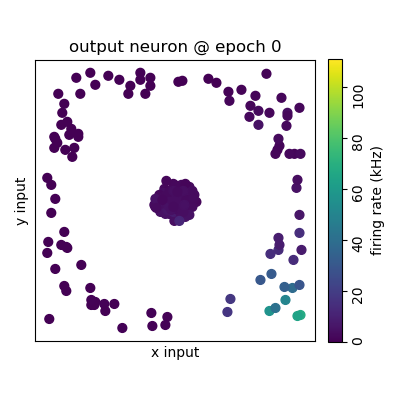
\includegraphics[scale=0.20]{mfp/learning_process/output_neuron_5.png}
				\label{cubesetup}
			\end{subfigure}
			\begin{subfigure}{0.3\textwidth}
				\centering
				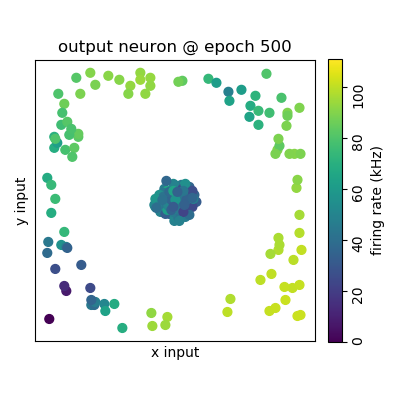
\includegraphics[scale=0.20]{mfp/learning_process/output_neuron_500.png}
				\label{cubesetup}
			\end{subfigure}	
			\begin{subfigure}{0.3\textwidth}
				\centering
				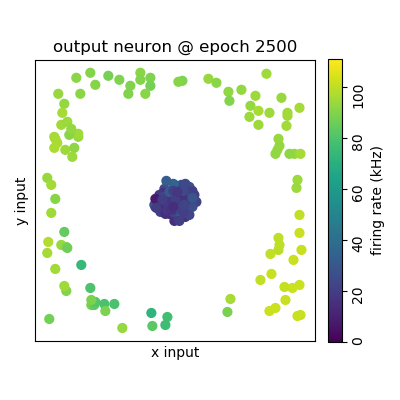
\includegraphics[scale=0.20]{mfp/learning_process/output_neuron_2500.png}
			\end{subfigure}
		    \end{figure}
		    
		\begin{figure}
		     	\vspace{-.7cm}
		     	\scalebox{0.8}{%% Creator: Matplotlib, PGF backend
%%
%% To include the figure in your LaTeX document, write
%%   \input{<filename>.pgf}
%%
%% Make sure the required packages are loaded in your preamble
%%   \usepackage{pgf}
%%
%% Figures using additional raster images can only be included by \input if
%% they are in the same directory as the main LaTeX file. For loading figures
%% from other directories you can use the `import` package
%%   \usepackage{import}
%% and then include the figures with
%%   \import{<path to file>}{<filename>.pgf}
%%
%% Matplotlib used the following preamble
%%   \usepackage{amsmath} \usepackage{pifont} \usepackage{xcolor} \definecolor{green}{HTML}{467821} \definecolor{red}{HTML}{CF4457} \usepackage[detect-all]{siunitx}
%%   \usepackage{fontspec}
%%
\begingroup%
\makeatletter%
\begin{pgfpicture}%
\pgfpathrectangle{\pgfpointorigin}{\pgfqpoint{3.256365in}{2.027862in}}%
\pgfusepath{use as bounding box, clip}%
\begin{pgfscope}%
\pgfsetbuttcap%
\pgfsetmiterjoin%
\pgfsetlinewidth{0.000000pt}%
\definecolor{currentstroke}{rgb}{0.000000,0.000000,0.000000}%
\pgfsetstrokecolor{currentstroke}%
\pgfsetstrokeopacity{0.000000}%
\pgfsetdash{}{0pt}%
\pgfpathmoveto{\pgfqpoint{0.000000in}{0.000000in}}%
\pgfpathlineto{\pgfqpoint{3.256365in}{0.000000in}}%
\pgfpathlineto{\pgfqpoint{3.256365in}{2.027862in}}%
\pgfpathlineto{\pgfqpoint{0.000000in}{2.027862in}}%
\pgfpathclose%
\pgfusepath{}%
\end{pgfscope}%
\begin{pgfscope}%
\pgfsetbuttcap%
\pgfsetmiterjoin%
\pgfsetlinewidth{0.000000pt}%
\definecolor{currentstroke}{rgb}{0.000000,0.000000,0.000000}%
\pgfsetstrokecolor{currentstroke}%
\pgfsetstrokeopacity{0.000000}%
\pgfsetdash{}{0pt}%
\pgfpathmoveto{\pgfqpoint{0.443865in}{1.217314in}}%
\pgfpathlineto{\pgfqpoint{3.156365in}{1.217314in}}%
\pgfpathlineto{\pgfqpoint{3.156365in}{1.919640in}}%
\pgfpathlineto{\pgfqpoint{0.443865in}{1.919640in}}%
\pgfpathclose%
\pgfusepath{}%
\end{pgfscope}%
\begin{pgfscope}%
\pgfsetbuttcap%
\pgfsetroundjoin%
\definecolor{currentfill}{rgb}{0.317647,0.317647,0.317647}%
\pgfsetfillcolor{currentfill}%
\pgfsetlinewidth{0.501875pt}%
\definecolor{currentstroke}{rgb}{0.317647,0.317647,0.317647}%
\pgfsetstrokecolor{currentstroke}%
\pgfsetdash{}{0pt}%
\pgfsys@defobject{currentmarker}{\pgfqpoint{0.000000in}{-0.020833in}}{\pgfqpoint{0.000000in}{0.000000in}}{%
\pgfpathmoveto{\pgfqpoint{0.000000in}{0.000000in}}%
\pgfpathlineto{\pgfqpoint{0.000000in}{-0.020833in}}%
\pgfusepath{stroke,fill}%
}%
\begin{pgfscope}%
\pgfsys@transformshift{0.567161in}{1.217314in}%
\pgfsys@useobject{currentmarker}{}%
\end{pgfscope}%
\end{pgfscope}%
\begin{pgfscope}%
\pgfsetbuttcap%
\pgfsetroundjoin%
\definecolor{currentfill}{rgb}{0.317647,0.317647,0.317647}%
\pgfsetfillcolor{currentfill}%
\pgfsetlinewidth{0.501875pt}%
\definecolor{currentstroke}{rgb}{0.317647,0.317647,0.317647}%
\pgfsetstrokecolor{currentstroke}%
\pgfsetdash{}{0pt}%
\pgfsys@defobject{currentmarker}{\pgfqpoint{0.000000in}{-0.020833in}}{\pgfqpoint{0.000000in}{0.000000in}}{%
\pgfpathmoveto{\pgfqpoint{0.000000in}{0.000000in}}%
\pgfpathlineto{\pgfqpoint{0.000000in}{-0.020833in}}%
\pgfusepath{stroke,fill}%
}%
\begin{pgfscope}%
\pgfsys@transformshift{1.061331in}{1.217314in}%
\pgfsys@useobject{currentmarker}{}%
\end{pgfscope}%
\end{pgfscope}%
\begin{pgfscope}%
\pgfsetbuttcap%
\pgfsetroundjoin%
\definecolor{currentfill}{rgb}{0.317647,0.317647,0.317647}%
\pgfsetfillcolor{currentfill}%
\pgfsetlinewidth{0.501875pt}%
\definecolor{currentstroke}{rgb}{0.317647,0.317647,0.317647}%
\pgfsetstrokecolor{currentstroke}%
\pgfsetdash{}{0pt}%
\pgfsys@defobject{currentmarker}{\pgfqpoint{0.000000in}{-0.020833in}}{\pgfqpoint{0.000000in}{0.000000in}}{%
\pgfpathmoveto{\pgfqpoint{0.000000in}{0.000000in}}%
\pgfpathlineto{\pgfqpoint{0.000000in}{-0.020833in}}%
\pgfusepath{stroke,fill}%
}%
\begin{pgfscope}%
\pgfsys@transformshift{1.555501in}{1.217314in}%
\pgfsys@useobject{currentmarker}{}%
\end{pgfscope}%
\end{pgfscope}%
\begin{pgfscope}%
\pgfsetbuttcap%
\pgfsetroundjoin%
\definecolor{currentfill}{rgb}{0.317647,0.317647,0.317647}%
\pgfsetfillcolor{currentfill}%
\pgfsetlinewidth{0.501875pt}%
\definecolor{currentstroke}{rgb}{0.317647,0.317647,0.317647}%
\pgfsetstrokecolor{currentstroke}%
\pgfsetdash{}{0pt}%
\pgfsys@defobject{currentmarker}{\pgfqpoint{0.000000in}{-0.020833in}}{\pgfqpoint{0.000000in}{0.000000in}}{%
\pgfpathmoveto{\pgfqpoint{0.000000in}{0.000000in}}%
\pgfpathlineto{\pgfqpoint{0.000000in}{-0.020833in}}%
\pgfusepath{stroke,fill}%
}%
\begin{pgfscope}%
\pgfsys@transformshift{2.049671in}{1.217314in}%
\pgfsys@useobject{currentmarker}{}%
\end{pgfscope}%
\end{pgfscope}%
\begin{pgfscope}%
\pgfsetbuttcap%
\pgfsetroundjoin%
\definecolor{currentfill}{rgb}{0.317647,0.317647,0.317647}%
\pgfsetfillcolor{currentfill}%
\pgfsetlinewidth{0.501875pt}%
\definecolor{currentstroke}{rgb}{0.317647,0.317647,0.317647}%
\pgfsetstrokecolor{currentstroke}%
\pgfsetdash{}{0pt}%
\pgfsys@defobject{currentmarker}{\pgfqpoint{0.000000in}{-0.020833in}}{\pgfqpoint{0.000000in}{0.000000in}}{%
\pgfpathmoveto{\pgfqpoint{0.000000in}{0.000000in}}%
\pgfpathlineto{\pgfqpoint{0.000000in}{-0.020833in}}%
\pgfusepath{stroke,fill}%
}%
\begin{pgfscope}%
\pgfsys@transformshift{2.543841in}{1.217314in}%
\pgfsys@useobject{currentmarker}{}%
\end{pgfscope}%
\end{pgfscope}%
\begin{pgfscope}%
\pgfsetbuttcap%
\pgfsetroundjoin%
\definecolor{currentfill}{rgb}{0.317647,0.317647,0.317647}%
\pgfsetfillcolor{currentfill}%
\pgfsetlinewidth{0.501875pt}%
\definecolor{currentstroke}{rgb}{0.317647,0.317647,0.317647}%
\pgfsetstrokecolor{currentstroke}%
\pgfsetdash{}{0pt}%
\pgfsys@defobject{currentmarker}{\pgfqpoint{0.000000in}{-0.020833in}}{\pgfqpoint{0.000000in}{0.000000in}}{%
\pgfpathmoveto{\pgfqpoint{0.000000in}{0.000000in}}%
\pgfpathlineto{\pgfqpoint{0.000000in}{-0.020833in}}%
\pgfusepath{stroke,fill}%
}%
\begin{pgfscope}%
\pgfsys@transformshift{3.038012in}{1.217314in}%
\pgfsys@useobject{currentmarker}{}%
\end{pgfscope}%
\end{pgfscope}%
\begin{pgfscope}%
\pgfsetbuttcap%
\pgfsetroundjoin%
\definecolor{currentfill}{rgb}{0.317647,0.317647,0.317647}%
\pgfsetfillcolor{currentfill}%
\pgfsetlinewidth{0.501875pt}%
\definecolor{currentstroke}{rgb}{0.317647,0.317647,0.317647}%
\pgfsetstrokecolor{currentstroke}%
\pgfsetdash{}{0pt}%
\pgfsys@defobject{currentmarker}{\pgfqpoint{-0.020833in}{0.000000in}}{\pgfqpoint{0.000000in}{0.000000in}}{%
\pgfpathmoveto{\pgfqpoint{0.000000in}{0.000000in}}%
\pgfpathlineto{\pgfqpoint{-0.020833in}{0.000000in}}%
\pgfusepath{stroke,fill}%
}%
\begin{pgfscope}%
\pgfsys@transformshift{0.443865in}{1.512141in}%
\pgfsys@useobject{currentmarker}{}%
\end{pgfscope}%
\end{pgfscope}%
\begin{pgfscope}%
\definecolor{textcolor}{rgb}{0.317647,0.317647,0.317647}%
\pgfsetstrokecolor{textcolor}%
\pgfsetfillcolor{textcolor}%
\pgftext[x=0.258292in,y=1.471995in,left,base]{\color{textcolor}\rmfamily\fontsize{8.330000}{9.996000}\selectfont \(\displaystyle 0.5\)}%
\end{pgfscope}%
\begin{pgfscope}%
\pgfsetbuttcap%
\pgfsetroundjoin%
\definecolor{currentfill}{rgb}{0.317647,0.317647,0.317647}%
\pgfsetfillcolor{currentfill}%
\pgfsetlinewidth{0.501875pt}%
\definecolor{currentstroke}{rgb}{0.317647,0.317647,0.317647}%
\pgfsetstrokecolor{currentstroke}%
\pgfsetdash{}{0pt}%
\pgfsys@defobject{currentmarker}{\pgfqpoint{-0.020833in}{0.000000in}}{\pgfqpoint{0.000000in}{0.000000in}}{%
\pgfpathmoveto{\pgfqpoint{0.000000in}{0.000000in}}%
\pgfpathlineto{\pgfqpoint{-0.020833in}{0.000000in}}%
\pgfusepath{stroke,fill}%
}%
\begin{pgfscope}%
\pgfsys@transformshift{0.443865in}{1.887716in}%
\pgfsys@useobject{currentmarker}{}%
\end{pgfscope}%
\end{pgfscope}%
\begin{pgfscope}%
\definecolor{textcolor}{rgb}{0.317647,0.317647,0.317647}%
\pgfsetstrokecolor{textcolor}%
\pgfsetfillcolor{textcolor}%
\pgftext[x=0.258292in,y=1.847570in,left,base]{\color{textcolor}\rmfamily\fontsize{8.330000}{9.996000}\selectfont \(\displaystyle 1.0\)}%
\end{pgfscope}%
\begin{pgfscope}%
\definecolor{textcolor}{rgb}{0.317647,0.317647,0.317647}%
\pgfsetstrokecolor{textcolor}%
\pgfsetfillcolor{textcolor}%
\pgftext[x=0.202737in,y=1.568477in,,bottom,rotate=90.000000]{\color{textcolor}\rmfamily\fontsize{8.330000}{9.996000}\selectfont accuracy}%
\end{pgfscope}%
\begin{pgfscope}%
\pgfpathrectangle{\pgfqpoint{0.443865in}{1.217314in}}{\pgfqpoint{2.712500in}{0.702326in}}%
\pgfusepath{clip}%
\pgfsetrectcap%
\pgfsetroundjoin%
\pgfsetlinewidth{0.803000pt}%
\definecolor{currentstroke}{rgb}{0.333333,0.333333,0.333333}%
\pgfsetstrokecolor{currentstroke}%
\pgfsetdash{}{0pt}%
\pgfpathmoveto{\pgfqpoint{0.567161in}{1.500873in}}%
\pgfpathlineto{\pgfqpoint{0.572102in}{1.512141in}}%
\pgfpathlineto{\pgfqpoint{0.577044in}{1.515896in}}%
\pgfpathlineto{\pgfqpoint{0.581986in}{1.530919in}}%
\pgfpathlineto{\pgfqpoint{0.586928in}{1.459560in}}%
\pgfpathlineto{\pgfqpoint{0.591869in}{1.568477in}}%
\pgfpathlineto{\pgfqpoint{0.596811in}{1.553454in}}%
\pgfpathlineto{\pgfqpoint{0.601753in}{1.560965in}}%
\pgfpathlineto{\pgfqpoint{0.606694in}{1.553454in}}%
\pgfpathlineto{\pgfqpoint{0.616578in}{1.560965in}}%
\pgfpathlineto{\pgfqpoint{0.621519in}{1.572233in}}%
\pgfpathlineto{\pgfqpoint{0.626461in}{1.560965in}}%
\pgfpathlineto{\pgfqpoint{0.631403in}{1.515896in}}%
\pgfpathlineto{\pgfqpoint{0.636345in}{1.361911in}}%
\pgfpathlineto{\pgfqpoint{0.641286in}{1.493362in}}%
\pgfpathlineto{\pgfqpoint{0.646228in}{1.534675in}}%
\pgfpathlineto{\pgfqpoint{0.651170in}{1.249238in}}%
\pgfpathlineto{\pgfqpoint{0.656111in}{1.275528in}}%
\pgfpathlineto{\pgfqpoint{0.661053in}{1.523408in}}%
\pgfpathlineto{\pgfqpoint{0.665995in}{1.418247in}}%
\pgfpathlineto{\pgfqpoint{0.670936in}{1.568477in}}%
\pgfpathlineto{\pgfqpoint{0.675878in}{1.444537in}}%
\pgfpathlineto{\pgfqpoint{0.680820in}{1.545942in}}%
\pgfpathlineto{\pgfqpoint{0.685762in}{1.598523in}}%
\pgfpathlineto{\pgfqpoint{0.690703in}{1.485850in}}%
\pgfpathlineto{\pgfqpoint{0.695645in}{1.591011in}}%
\pgfpathlineto{\pgfqpoint{0.700587in}{1.369422in}}%
\pgfpathlineto{\pgfqpoint{0.705528in}{1.316842in}}%
\pgfpathlineto{\pgfqpoint{0.710470in}{1.350643in}}%
\pgfpathlineto{\pgfqpoint{0.715412in}{1.621057in}}%
\pgfpathlineto{\pgfqpoint{0.720353in}{1.617302in}}%
\pgfpathlineto{\pgfqpoint{0.725295in}{1.688661in}}%
\pgfpathlineto{\pgfqpoint{0.730237in}{1.718707in}}%
\pgfpathlineto{\pgfqpoint{0.740120in}{1.718707in}}%
\pgfpathlineto{\pgfqpoint{0.745062in}{1.485850in}}%
\pgfpathlineto{\pgfqpoint{0.750004in}{1.714951in}}%
\pgfpathlineto{\pgfqpoint{0.754945in}{1.666126in}}%
\pgfpathlineto{\pgfqpoint{0.759887in}{1.643592in}}%
\pgfpathlineto{\pgfqpoint{0.764829in}{1.688661in}}%
\pgfpathlineto{\pgfqpoint{0.769770in}{1.658615in}}%
\pgfpathlineto{\pgfqpoint{0.779654in}{1.418247in}}%
\pgfpathlineto{\pgfqpoint{0.784596in}{1.388201in}}%
\pgfpathlineto{\pgfqpoint{0.789537in}{1.418247in}}%
\pgfpathlineto{\pgfqpoint{0.794479in}{1.410735in}}%
\pgfpathlineto{\pgfqpoint{0.799421in}{1.444537in}}%
\pgfpathlineto{\pgfqpoint{0.804362in}{1.560965in}}%
\pgfpathlineto{\pgfqpoint{0.814246in}{1.673638in}}%
\pgfpathlineto{\pgfqpoint{0.819188in}{1.677394in}}%
\pgfpathlineto{\pgfqpoint{0.824129in}{1.790066in}}%
\pgfpathlineto{\pgfqpoint{0.829071in}{1.692417in}}%
\pgfpathlineto{\pgfqpoint{0.834013in}{1.628569in}}%
\pgfpathlineto{\pgfqpoint{0.838954in}{1.647348in}}%
\pgfpathlineto{\pgfqpoint{0.843896in}{1.790066in}}%
\pgfpathlineto{\pgfqpoint{0.848838in}{1.778799in}}%
\pgfpathlineto{\pgfqpoint{0.853779in}{1.726219in}}%
\pgfpathlineto{\pgfqpoint{0.858721in}{1.714951in}}%
\pgfpathlineto{\pgfqpoint{0.863663in}{1.718707in}}%
\pgfpathlineto{\pgfqpoint{0.868605in}{1.729974in}}%
\pgfpathlineto{\pgfqpoint{0.873546in}{1.756265in}}%
\pgfpathlineto{\pgfqpoint{0.878488in}{1.677394in}}%
\pgfpathlineto{\pgfqpoint{0.883430in}{1.775043in}}%
\pgfpathlineto{\pgfqpoint{0.888371in}{1.756265in}}%
\pgfpathlineto{\pgfqpoint{0.893313in}{1.748753in}}%
\pgfpathlineto{\pgfqpoint{0.898255in}{1.737486in}}%
\pgfpathlineto{\pgfqpoint{0.903196in}{1.771288in}}%
\pgfpathlineto{\pgfqpoint{0.908138in}{1.760020in}}%
\pgfpathlineto{\pgfqpoint{0.913080in}{1.756265in}}%
\pgfpathlineto{\pgfqpoint{0.918022in}{1.756265in}}%
\pgfpathlineto{\pgfqpoint{0.922963in}{1.790066in}}%
\pgfpathlineto{\pgfqpoint{0.927905in}{1.786311in}}%
\pgfpathlineto{\pgfqpoint{0.932847in}{1.763776in}}%
\pgfpathlineto{\pgfqpoint{0.937788in}{1.801334in}}%
\pgfpathlineto{\pgfqpoint{0.942730in}{1.797578in}}%
\pgfpathlineto{\pgfqpoint{0.947672in}{1.790066in}}%
\pgfpathlineto{\pgfqpoint{0.952613in}{1.677394in}}%
\pgfpathlineto{\pgfqpoint{0.957555in}{1.771288in}}%
\pgfpathlineto{\pgfqpoint{0.962497in}{1.778799in}}%
\pgfpathlineto{\pgfqpoint{0.967439in}{1.767532in}}%
\pgfpathlineto{\pgfqpoint{0.972380in}{1.748753in}}%
\pgfpathlineto{\pgfqpoint{0.977322in}{1.703684in}}%
\pgfpathlineto{\pgfqpoint{0.982264in}{1.737486in}}%
\pgfpathlineto{\pgfqpoint{0.987205in}{1.748753in}}%
\pgfpathlineto{\pgfqpoint{0.992147in}{1.729974in}}%
\pgfpathlineto{\pgfqpoint{0.997089in}{1.733730in}}%
\pgfpathlineto{\pgfqpoint{1.002030in}{1.756265in}}%
\pgfpathlineto{\pgfqpoint{1.006972in}{1.647348in}}%
\pgfpathlineto{\pgfqpoint{1.011914in}{1.756265in}}%
\pgfpathlineto{\pgfqpoint{1.016856in}{1.775043in}}%
\pgfpathlineto{\pgfqpoint{1.021797in}{1.666126in}}%
\pgfpathlineto{\pgfqpoint{1.026739in}{1.748753in}}%
\pgfpathlineto{\pgfqpoint{1.031681in}{1.756265in}}%
\pgfpathlineto{\pgfqpoint{1.036622in}{1.778799in}}%
\pgfpathlineto{\pgfqpoint{1.041564in}{1.632325in}}%
\pgfpathlineto{\pgfqpoint{1.046506in}{1.767532in}}%
\pgfpathlineto{\pgfqpoint{1.051447in}{1.775043in}}%
\pgfpathlineto{\pgfqpoint{1.056389in}{1.786311in}}%
\pgfpathlineto{\pgfqpoint{1.061331in}{1.756265in}}%
\pgfpathlineto{\pgfqpoint{1.066273in}{1.699928in}}%
\pgfpathlineto{\pgfqpoint{1.071214in}{1.669882in}}%
\pgfpathlineto{\pgfqpoint{1.076156in}{1.617302in}}%
\pgfpathlineto{\pgfqpoint{1.081098in}{1.606034in}}%
\pgfpathlineto{\pgfqpoint{1.086039in}{1.639836in}}%
\pgfpathlineto{\pgfqpoint{1.090981in}{1.639836in}}%
\pgfpathlineto{\pgfqpoint{1.095923in}{1.591011in}}%
\pgfpathlineto{\pgfqpoint{1.100865in}{1.594767in}}%
\pgfpathlineto{\pgfqpoint{1.105806in}{1.602279in}}%
\pgfpathlineto{\pgfqpoint{1.110748in}{1.639836in}}%
\pgfpathlineto{\pgfqpoint{1.115690in}{1.613546in}}%
\pgfpathlineto{\pgfqpoint{1.120631in}{1.613546in}}%
\pgfpathlineto{\pgfqpoint{1.125573in}{1.606034in}}%
\pgfpathlineto{\pgfqpoint{1.130515in}{1.643592in}}%
\pgfpathlineto{\pgfqpoint{1.135456in}{1.666126in}}%
\pgfpathlineto{\pgfqpoint{1.140398in}{1.621057in}}%
\pgfpathlineto{\pgfqpoint{1.145340in}{1.621057in}}%
\pgfpathlineto{\pgfqpoint{1.150282in}{1.681149in}}%
\pgfpathlineto{\pgfqpoint{1.155223in}{1.666126in}}%
\pgfpathlineto{\pgfqpoint{1.160165in}{1.741242in}}%
\pgfpathlineto{\pgfqpoint{1.165107in}{1.711195in}}%
\pgfpathlineto{\pgfqpoint{1.170048in}{1.632325in}}%
\pgfpathlineto{\pgfqpoint{1.174990in}{1.729974in}}%
\pgfpathlineto{\pgfqpoint{1.179932in}{1.714951in}}%
\pgfpathlineto{\pgfqpoint{1.184873in}{1.643592in}}%
\pgfpathlineto{\pgfqpoint{1.189815in}{1.714951in}}%
\pgfpathlineto{\pgfqpoint{1.194757in}{1.651103in}}%
\pgfpathlineto{\pgfqpoint{1.199699in}{1.744997in}}%
\pgfpathlineto{\pgfqpoint{1.204640in}{1.726219in}}%
\pgfpathlineto{\pgfqpoint{1.209582in}{1.658615in}}%
\pgfpathlineto{\pgfqpoint{1.214524in}{1.621057in}}%
\pgfpathlineto{\pgfqpoint{1.219465in}{1.628569in}}%
\pgfpathlineto{\pgfqpoint{1.224407in}{1.677394in}}%
\pgfpathlineto{\pgfqpoint{1.229349in}{1.677394in}}%
\pgfpathlineto{\pgfqpoint{1.234290in}{1.654859in}}%
\pgfpathlineto{\pgfqpoint{1.239232in}{1.722463in}}%
\pgfpathlineto{\pgfqpoint{1.244174in}{1.726219in}}%
\pgfpathlineto{\pgfqpoint{1.254057in}{1.707440in}}%
\pgfpathlineto{\pgfqpoint{1.258999in}{1.714951in}}%
\pgfpathlineto{\pgfqpoint{1.263941in}{1.744997in}}%
\pgfpathlineto{\pgfqpoint{1.268882in}{1.729974in}}%
\pgfpathlineto{\pgfqpoint{1.273824in}{1.756265in}}%
\pgfpathlineto{\pgfqpoint{1.278766in}{1.760020in}}%
\pgfpathlineto{\pgfqpoint{1.283707in}{1.760020in}}%
\pgfpathlineto{\pgfqpoint{1.288649in}{1.767532in}}%
\pgfpathlineto{\pgfqpoint{1.293591in}{1.741242in}}%
\pgfpathlineto{\pgfqpoint{1.298533in}{1.775043in}}%
\pgfpathlineto{\pgfqpoint{1.303474in}{1.767532in}}%
\pgfpathlineto{\pgfqpoint{1.308416in}{1.767532in}}%
\pgfpathlineto{\pgfqpoint{1.313358in}{1.771288in}}%
\pgfpathlineto{\pgfqpoint{1.318299in}{1.752509in}}%
\pgfpathlineto{\pgfqpoint{1.323241in}{1.744997in}}%
\pgfpathlineto{\pgfqpoint{1.328183in}{1.722463in}}%
\pgfpathlineto{\pgfqpoint{1.333124in}{1.744997in}}%
\pgfpathlineto{\pgfqpoint{1.338066in}{1.722463in}}%
\pgfpathlineto{\pgfqpoint{1.347950in}{1.756265in}}%
\pgfpathlineto{\pgfqpoint{1.352891in}{1.805089in}}%
\pgfpathlineto{\pgfqpoint{1.357833in}{1.786311in}}%
\pgfpathlineto{\pgfqpoint{1.362775in}{1.812601in}}%
\pgfpathlineto{\pgfqpoint{1.367716in}{1.775043in}}%
\pgfpathlineto{\pgfqpoint{1.372658in}{1.756265in}}%
\pgfpathlineto{\pgfqpoint{1.377600in}{1.756265in}}%
\pgfpathlineto{\pgfqpoint{1.382541in}{1.778799in}}%
\pgfpathlineto{\pgfqpoint{1.387483in}{1.793822in}}%
\pgfpathlineto{\pgfqpoint{1.392425in}{1.489606in}}%
\pgfpathlineto{\pgfqpoint{1.397367in}{1.808845in}}%
\pgfpathlineto{\pgfqpoint{1.402308in}{1.775043in}}%
\pgfpathlineto{\pgfqpoint{1.407250in}{1.752509in}}%
\pgfpathlineto{\pgfqpoint{1.412192in}{1.786311in}}%
\pgfpathlineto{\pgfqpoint{1.417133in}{1.782555in}}%
\pgfpathlineto{\pgfqpoint{1.422075in}{1.744997in}}%
\pgfpathlineto{\pgfqpoint{1.427017in}{1.775043in}}%
\pgfpathlineto{\pgfqpoint{1.431959in}{1.718707in}}%
\pgfpathlineto{\pgfqpoint{1.436900in}{1.763776in}}%
\pgfpathlineto{\pgfqpoint{1.441842in}{1.760020in}}%
\pgfpathlineto{\pgfqpoint{1.446784in}{1.771288in}}%
\pgfpathlineto{\pgfqpoint{1.456667in}{1.771288in}}%
\pgfpathlineto{\pgfqpoint{1.461609in}{1.778799in}}%
\pgfpathlineto{\pgfqpoint{1.466550in}{1.782555in}}%
\pgfpathlineto{\pgfqpoint{1.471492in}{1.729974in}}%
\pgfpathlineto{\pgfqpoint{1.476434in}{1.778799in}}%
\pgfpathlineto{\pgfqpoint{1.481376in}{1.523408in}}%
\pgfpathlineto{\pgfqpoint{1.486317in}{1.793822in}}%
\pgfpathlineto{\pgfqpoint{1.506084in}{1.778799in}}%
\pgfpathlineto{\pgfqpoint{1.511026in}{1.763776in}}%
\pgfpathlineto{\pgfqpoint{1.515967in}{1.771288in}}%
\pgfpathlineto{\pgfqpoint{1.520909in}{1.771288in}}%
\pgfpathlineto{\pgfqpoint{1.525851in}{1.797578in}}%
\pgfpathlineto{\pgfqpoint{1.530793in}{1.684905in}}%
\pgfpathlineto{\pgfqpoint{1.540676in}{1.805089in}}%
\pgfpathlineto{\pgfqpoint{1.545618in}{1.775043in}}%
\pgfpathlineto{\pgfqpoint{1.550559in}{1.805089in}}%
\pgfpathlineto{\pgfqpoint{1.555501in}{1.790066in}}%
\pgfpathlineto{\pgfqpoint{1.560443in}{1.786311in}}%
\pgfpathlineto{\pgfqpoint{1.565384in}{1.778799in}}%
\pgfpathlineto{\pgfqpoint{1.570326in}{1.752509in}}%
\pgfpathlineto{\pgfqpoint{1.575268in}{1.790066in}}%
\pgfpathlineto{\pgfqpoint{1.580210in}{1.782555in}}%
\pgfpathlineto{\pgfqpoint{1.585151in}{1.808845in}}%
\pgfpathlineto{\pgfqpoint{1.590093in}{1.797578in}}%
\pgfpathlineto{\pgfqpoint{1.595035in}{1.801334in}}%
\pgfpathlineto{\pgfqpoint{1.599976in}{1.790066in}}%
\pgfpathlineto{\pgfqpoint{1.604918in}{1.786311in}}%
\pgfpathlineto{\pgfqpoint{1.609860in}{1.835135in}}%
\pgfpathlineto{\pgfqpoint{1.614801in}{1.816357in}}%
\pgfpathlineto{\pgfqpoint{1.619743in}{1.767532in}}%
\pgfpathlineto{\pgfqpoint{1.624685in}{1.797578in}}%
\pgfpathlineto{\pgfqpoint{1.629627in}{1.786311in}}%
\pgfpathlineto{\pgfqpoint{1.634568in}{1.801334in}}%
\pgfpathlineto{\pgfqpoint{1.639510in}{1.805089in}}%
\pgfpathlineto{\pgfqpoint{1.644452in}{1.775043in}}%
\pgfpathlineto{\pgfqpoint{1.649393in}{1.827624in}}%
\pgfpathlineto{\pgfqpoint{1.654335in}{1.835135in}}%
\pgfpathlineto{\pgfqpoint{1.664218in}{1.820112in}}%
\pgfpathlineto{\pgfqpoint{1.669160in}{1.797578in}}%
\pgfpathlineto{\pgfqpoint{1.674102in}{1.823868in}}%
\pgfpathlineto{\pgfqpoint{1.679044in}{1.816357in}}%
\pgfpathlineto{\pgfqpoint{1.688927in}{1.673638in}}%
\pgfpathlineto{\pgfqpoint{1.693869in}{1.778799in}}%
\pgfpathlineto{\pgfqpoint{1.698810in}{1.786311in}}%
\pgfpathlineto{\pgfqpoint{1.703752in}{1.786311in}}%
\pgfpathlineto{\pgfqpoint{1.708694in}{1.790066in}}%
\pgfpathlineto{\pgfqpoint{1.713636in}{1.771288in}}%
\pgfpathlineto{\pgfqpoint{1.718577in}{1.782555in}}%
\pgfpathlineto{\pgfqpoint{1.723519in}{1.786311in}}%
\pgfpathlineto{\pgfqpoint{1.728461in}{1.782555in}}%
\pgfpathlineto{\pgfqpoint{1.733402in}{1.790066in}}%
\pgfpathlineto{\pgfqpoint{1.738344in}{1.763776in}}%
\pgfpathlineto{\pgfqpoint{1.743286in}{1.793822in}}%
\pgfpathlineto{\pgfqpoint{1.748227in}{1.793822in}}%
\pgfpathlineto{\pgfqpoint{1.753169in}{1.771288in}}%
\pgfpathlineto{\pgfqpoint{1.758111in}{1.808845in}}%
\pgfpathlineto{\pgfqpoint{1.763053in}{1.763776in}}%
\pgfpathlineto{\pgfqpoint{1.767994in}{1.805089in}}%
\pgfpathlineto{\pgfqpoint{1.772936in}{1.812601in}}%
\pgfpathlineto{\pgfqpoint{1.777878in}{1.797578in}}%
\pgfpathlineto{\pgfqpoint{1.787761in}{1.790066in}}%
\pgfpathlineto{\pgfqpoint{1.797644in}{1.790066in}}%
\pgfpathlineto{\pgfqpoint{1.802586in}{1.782555in}}%
\pgfpathlineto{\pgfqpoint{1.807528in}{1.797578in}}%
\pgfpathlineto{\pgfqpoint{1.812470in}{1.793822in}}%
\pgfpathlineto{\pgfqpoint{1.817411in}{1.782555in}}%
\pgfpathlineto{\pgfqpoint{1.822353in}{1.790066in}}%
\pgfpathlineto{\pgfqpoint{1.827295in}{1.786311in}}%
\pgfpathlineto{\pgfqpoint{1.832236in}{1.786311in}}%
\pgfpathlineto{\pgfqpoint{1.837178in}{1.812601in}}%
\pgfpathlineto{\pgfqpoint{1.847061in}{1.812601in}}%
\pgfpathlineto{\pgfqpoint{1.852003in}{1.778799in}}%
\pgfpathlineto{\pgfqpoint{1.856945in}{1.756265in}}%
\pgfpathlineto{\pgfqpoint{1.861887in}{1.778799in}}%
\pgfpathlineto{\pgfqpoint{1.866828in}{1.703684in}}%
\pgfpathlineto{\pgfqpoint{1.871770in}{1.797578in}}%
\pgfpathlineto{\pgfqpoint{1.876712in}{1.820112in}}%
\pgfpathlineto{\pgfqpoint{1.881653in}{1.808845in}}%
\pgfpathlineto{\pgfqpoint{1.896478in}{1.808845in}}%
\pgfpathlineto{\pgfqpoint{1.906362in}{1.801334in}}%
\pgfpathlineto{\pgfqpoint{1.911304in}{1.782555in}}%
\pgfpathlineto{\pgfqpoint{1.916245in}{1.771288in}}%
\pgfpathlineto{\pgfqpoint{1.921187in}{1.786311in}}%
\pgfpathlineto{\pgfqpoint{1.926129in}{1.782555in}}%
\pgfpathlineto{\pgfqpoint{1.931070in}{1.790066in}}%
\pgfpathlineto{\pgfqpoint{1.936012in}{1.823868in}}%
\pgfpathlineto{\pgfqpoint{1.940954in}{1.820112in}}%
\pgfpathlineto{\pgfqpoint{1.945895in}{1.805089in}}%
\pgfpathlineto{\pgfqpoint{1.950837in}{1.808845in}}%
\pgfpathlineto{\pgfqpoint{1.955779in}{1.808845in}}%
\pgfpathlineto{\pgfqpoint{1.960721in}{1.801334in}}%
\pgfpathlineto{\pgfqpoint{1.965662in}{1.726219in}}%
\pgfpathlineto{\pgfqpoint{1.970604in}{1.820112in}}%
\pgfpathlineto{\pgfqpoint{1.975546in}{1.816357in}}%
\pgfpathlineto{\pgfqpoint{1.980487in}{1.831380in}}%
\pgfpathlineto{\pgfqpoint{1.985429in}{1.823868in}}%
\pgfpathlineto{\pgfqpoint{1.990371in}{1.842647in}}%
\pgfpathlineto{\pgfqpoint{1.995312in}{1.778799in}}%
\pgfpathlineto{\pgfqpoint{2.000254in}{1.831380in}}%
\pgfpathlineto{\pgfqpoint{2.005196in}{1.850158in}}%
\pgfpathlineto{\pgfqpoint{2.010138in}{1.842647in}}%
\pgfpathlineto{\pgfqpoint{2.015079in}{1.827624in}}%
\pgfpathlineto{\pgfqpoint{2.024963in}{1.820112in}}%
\pgfpathlineto{\pgfqpoint{2.029904in}{1.831380in}}%
\pgfpathlineto{\pgfqpoint{2.034846in}{1.820112in}}%
\pgfpathlineto{\pgfqpoint{2.039788in}{1.823868in}}%
\pgfpathlineto{\pgfqpoint{2.044730in}{1.842647in}}%
\pgfpathlineto{\pgfqpoint{2.049671in}{1.820112in}}%
\pgfpathlineto{\pgfqpoint{2.054613in}{1.838891in}}%
\pgfpathlineto{\pgfqpoint{2.064496in}{1.831380in}}%
\pgfpathlineto{\pgfqpoint{2.069438in}{1.835135in}}%
\pgfpathlineto{\pgfqpoint{2.074380in}{1.842647in}}%
\pgfpathlineto{\pgfqpoint{2.079321in}{1.816357in}}%
\pgfpathlineto{\pgfqpoint{2.084263in}{1.816357in}}%
\pgfpathlineto{\pgfqpoint{2.104030in}{1.801334in}}%
\pgfpathlineto{\pgfqpoint{2.108972in}{1.609790in}}%
\pgfpathlineto{\pgfqpoint{2.113913in}{1.816357in}}%
\pgfpathlineto{\pgfqpoint{2.118855in}{1.805089in}}%
\pgfpathlineto{\pgfqpoint{2.123797in}{1.812601in}}%
\pgfpathlineto{\pgfqpoint{2.128738in}{1.808845in}}%
\pgfpathlineto{\pgfqpoint{2.133680in}{1.812601in}}%
\pgfpathlineto{\pgfqpoint{2.138622in}{1.733730in}}%
\pgfpathlineto{\pgfqpoint{2.143564in}{1.688661in}}%
\pgfpathlineto{\pgfqpoint{2.148505in}{1.729974in}}%
\pgfpathlineto{\pgfqpoint{2.153447in}{1.718707in}}%
\pgfpathlineto{\pgfqpoint{2.158389in}{1.790066in}}%
\pgfpathlineto{\pgfqpoint{2.163330in}{1.793822in}}%
\pgfpathlineto{\pgfqpoint{2.168272in}{1.801334in}}%
\pgfpathlineto{\pgfqpoint{2.173214in}{1.801334in}}%
\pgfpathlineto{\pgfqpoint{2.183097in}{1.782555in}}%
\pgfpathlineto{\pgfqpoint{2.192981in}{1.767532in}}%
\pgfpathlineto{\pgfqpoint{2.197922in}{1.790066in}}%
\pgfpathlineto{\pgfqpoint{2.202864in}{1.797578in}}%
\pgfpathlineto{\pgfqpoint{2.207806in}{1.801334in}}%
\pgfpathlineto{\pgfqpoint{2.217689in}{1.820112in}}%
\pgfpathlineto{\pgfqpoint{2.222631in}{1.808845in}}%
\pgfpathlineto{\pgfqpoint{2.227572in}{1.823868in}}%
\pgfpathlineto{\pgfqpoint{2.232514in}{1.808845in}}%
\pgfpathlineto{\pgfqpoint{2.237456in}{1.805089in}}%
\pgfpathlineto{\pgfqpoint{2.242398in}{1.793822in}}%
\pgfpathlineto{\pgfqpoint{2.247339in}{1.793822in}}%
\pgfpathlineto{\pgfqpoint{2.252281in}{1.801334in}}%
\pgfpathlineto{\pgfqpoint{2.257223in}{1.786311in}}%
\pgfpathlineto{\pgfqpoint{2.262164in}{1.805089in}}%
\pgfpathlineto{\pgfqpoint{2.267106in}{1.801334in}}%
\pgfpathlineto{\pgfqpoint{2.272048in}{1.801334in}}%
\pgfpathlineto{\pgfqpoint{2.276989in}{1.805089in}}%
\pgfpathlineto{\pgfqpoint{2.281931in}{1.820112in}}%
\pgfpathlineto{\pgfqpoint{2.286873in}{1.816357in}}%
\pgfpathlineto{\pgfqpoint{2.291815in}{1.831380in}}%
\pgfpathlineto{\pgfqpoint{2.296756in}{1.853914in}}%
\pgfpathlineto{\pgfqpoint{2.306640in}{1.808845in}}%
\pgfpathlineto{\pgfqpoint{2.311581in}{1.801334in}}%
\pgfpathlineto{\pgfqpoint{2.321465in}{1.801334in}}%
\pgfpathlineto{\pgfqpoint{2.326406in}{1.805089in}}%
\pgfpathlineto{\pgfqpoint{2.331348in}{1.805089in}}%
\pgfpathlineto{\pgfqpoint{2.336290in}{1.598523in}}%
\pgfpathlineto{\pgfqpoint{2.341232in}{1.647348in}}%
\pgfpathlineto{\pgfqpoint{2.346173in}{1.797578in}}%
\pgfpathlineto{\pgfqpoint{2.351115in}{1.797578in}}%
\pgfpathlineto{\pgfqpoint{2.356057in}{1.801334in}}%
\pgfpathlineto{\pgfqpoint{2.360998in}{1.801334in}}%
\pgfpathlineto{\pgfqpoint{2.370882in}{1.793822in}}%
\pgfpathlineto{\pgfqpoint{2.375824in}{1.808845in}}%
\pgfpathlineto{\pgfqpoint{2.380765in}{1.797578in}}%
\pgfpathlineto{\pgfqpoint{2.385707in}{1.801334in}}%
\pgfpathlineto{\pgfqpoint{2.390649in}{1.801334in}}%
\pgfpathlineto{\pgfqpoint{2.395590in}{1.805089in}}%
\pgfpathlineto{\pgfqpoint{2.400532in}{1.797578in}}%
\pgfpathlineto{\pgfqpoint{2.405474in}{1.793822in}}%
\pgfpathlineto{\pgfqpoint{2.410415in}{1.805089in}}%
\pgfpathlineto{\pgfqpoint{2.415357in}{1.790066in}}%
\pgfpathlineto{\pgfqpoint{2.420299in}{1.805089in}}%
\pgfpathlineto{\pgfqpoint{2.425241in}{1.797578in}}%
\pgfpathlineto{\pgfqpoint{2.430182in}{1.805089in}}%
\pgfpathlineto{\pgfqpoint{2.435124in}{1.823868in}}%
\pgfpathlineto{\pgfqpoint{2.440066in}{1.823868in}}%
\pgfpathlineto{\pgfqpoint{2.445007in}{1.846403in}}%
\pgfpathlineto{\pgfqpoint{2.449949in}{1.808845in}}%
\pgfpathlineto{\pgfqpoint{2.454891in}{1.816357in}}%
\pgfpathlineto{\pgfqpoint{2.464774in}{1.801334in}}%
\pgfpathlineto{\pgfqpoint{2.469716in}{1.805089in}}%
\pgfpathlineto{\pgfqpoint{2.474658in}{1.790066in}}%
\pgfpathlineto{\pgfqpoint{2.479599in}{1.823868in}}%
\pgfpathlineto{\pgfqpoint{2.484541in}{1.805089in}}%
\pgfpathlineto{\pgfqpoint{2.489483in}{1.865181in}}%
\pgfpathlineto{\pgfqpoint{2.499366in}{1.707440in}}%
\pgfpathlineto{\pgfqpoint{2.504308in}{1.880204in}}%
\pgfpathlineto{\pgfqpoint{2.509249in}{1.876449in}}%
\pgfpathlineto{\pgfqpoint{2.519133in}{1.883960in}}%
\pgfpathlineto{\pgfqpoint{2.524075in}{1.876449in}}%
\pgfpathlineto{\pgfqpoint{2.529016in}{1.872693in}}%
\pgfpathlineto{\pgfqpoint{2.533958in}{1.887716in}}%
\pgfpathlineto{\pgfqpoint{2.538900in}{1.842647in}}%
\pgfpathlineto{\pgfqpoint{2.543841in}{1.887716in}}%
\pgfpathlineto{\pgfqpoint{2.573492in}{1.887716in}}%
\pgfpathlineto{\pgfqpoint{2.578433in}{1.876449in}}%
\pgfpathlineto{\pgfqpoint{2.583375in}{1.820112in}}%
\pgfpathlineto{\pgfqpoint{2.588317in}{1.816357in}}%
\pgfpathlineto{\pgfqpoint{2.593258in}{1.763776in}}%
\pgfpathlineto{\pgfqpoint{2.598200in}{1.831380in}}%
\pgfpathlineto{\pgfqpoint{2.603142in}{1.808845in}}%
\pgfpathlineto{\pgfqpoint{2.608083in}{1.838891in}}%
\pgfpathlineto{\pgfqpoint{2.613025in}{1.831380in}}%
\pgfpathlineto{\pgfqpoint{2.617967in}{1.846403in}}%
\pgfpathlineto{\pgfqpoint{2.622909in}{1.838891in}}%
\pgfpathlineto{\pgfqpoint{2.627850in}{1.887716in}}%
\pgfpathlineto{\pgfqpoint{2.637734in}{1.842647in}}%
\pgfpathlineto{\pgfqpoint{2.642675in}{1.868937in}}%
\pgfpathlineto{\pgfqpoint{2.647617in}{1.880204in}}%
\pgfpathlineto{\pgfqpoint{2.657501in}{1.887716in}}%
\pgfpathlineto{\pgfqpoint{2.662442in}{1.872693in}}%
\pgfpathlineto{\pgfqpoint{2.667384in}{1.838891in}}%
\pgfpathlineto{\pgfqpoint{2.672326in}{1.883960in}}%
\pgfpathlineto{\pgfqpoint{2.677267in}{1.880204in}}%
\pgfpathlineto{\pgfqpoint{2.682209in}{1.887716in}}%
\pgfpathlineto{\pgfqpoint{2.692092in}{1.880204in}}%
\pgfpathlineto{\pgfqpoint{2.697034in}{1.846403in}}%
\pgfpathlineto{\pgfqpoint{2.701976in}{1.887716in}}%
\pgfpathlineto{\pgfqpoint{2.706918in}{1.883960in}}%
\pgfpathlineto{\pgfqpoint{2.711859in}{1.883960in}}%
\pgfpathlineto{\pgfqpoint{2.716801in}{1.876449in}}%
\pgfpathlineto{\pgfqpoint{2.721743in}{1.846403in}}%
\pgfpathlineto{\pgfqpoint{2.726684in}{1.850158in}}%
\pgfpathlineto{\pgfqpoint{2.731626in}{1.842647in}}%
\pgfpathlineto{\pgfqpoint{2.736568in}{1.857670in}}%
\pgfpathlineto{\pgfqpoint{2.741509in}{1.857670in}}%
\pgfpathlineto{\pgfqpoint{2.756335in}{1.887716in}}%
\pgfpathlineto{\pgfqpoint{2.761276in}{1.883960in}}%
\pgfpathlineto{\pgfqpoint{2.766218in}{1.857670in}}%
\pgfpathlineto{\pgfqpoint{2.776101in}{1.850158in}}%
\pgfpathlineto{\pgfqpoint{2.781043in}{1.865181in}}%
\pgfpathlineto{\pgfqpoint{2.790926in}{1.880204in}}%
\pgfpathlineto{\pgfqpoint{2.800810in}{1.861426in}}%
\pgfpathlineto{\pgfqpoint{2.805752in}{1.883960in}}%
\pgfpathlineto{\pgfqpoint{2.810693in}{1.872693in}}%
\pgfpathlineto{\pgfqpoint{2.815635in}{1.883960in}}%
\pgfpathlineto{\pgfqpoint{2.820577in}{1.887716in}}%
\pgfpathlineto{\pgfqpoint{2.825518in}{1.861426in}}%
\pgfpathlineto{\pgfqpoint{2.830460in}{1.887716in}}%
\pgfpathlineto{\pgfqpoint{2.835402in}{1.887716in}}%
\pgfpathlineto{\pgfqpoint{2.840343in}{1.883960in}}%
\pgfpathlineto{\pgfqpoint{2.845285in}{1.887716in}}%
\pgfpathlineto{\pgfqpoint{2.855169in}{1.887716in}}%
\pgfpathlineto{\pgfqpoint{2.860110in}{1.883960in}}%
\pgfpathlineto{\pgfqpoint{2.865052in}{1.876449in}}%
\pgfpathlineto{\pgfqpoint{2.869994in}{1.883960in}}%
\pgfpathlineto{\pgfqpoint{2.874935in}{1.887716in}}%
\pgfpathlineto{\pgfqpoint{2.879877in}{1.887716in}}%
\pgfpathlineto{\pgfqpoint{2.884819in}{1.883960in}}%
\pgfpathlineto{\pgfqpoint{2.904586in}{1.883960in}}%
\pgfpathlineto{\pgfqpoint{2.909527in}{1.887716in}}%
\pgfpathlineto{\pgfqpoint{2.958944in}{1.887716in}}%
\pgfpathlineto{\pgfqpoint{2.963886in}{1.883960in}}%
\pgfpathlineto{\pgfqpoint{2.968828in}{1.887716in}}%
\pgfpathlineto{\pgfqpoint{2.978711in}{1.887716in}}%
\pgfpathlineto{\pgfqpoint{2.983653in}{1.883960in}}%
\pgfpathlineto{\pgfqpoint{2.998478in}{1.883960in}}%
\pgfpathlineto{\pgfqpoint{3.003420in}{1.887716in}}%
\pgfpathlineto{\pgfqpoint{3.033070in}{1.887716in}}%
\pgfpathlineto{\pgfqpoint{3.033070in}{1.887716in}}%
\pgfusepath{stroke}%
\end{pgfscope}%
\begin{pgfscope}%
\pgfsetrectcap%
\pgfsetmiterjoin%
\pgfsetlinewidth{0.501875pt}%
\definecolor{currentstroke}{rgb}{0.317647,0.317647,0.317647}%
\pgfsetstrokecolor{currentstroke}%
\pgfsetdash{}{0pt}%
\pgfpathmoveto{\pgfqpoint{0.443865in}{1.217314in}}%
\pgfpathlineto{\pgfqpoint{0.443865in}{1.919640in}}%
\pgfusepath{stroke}%
\end{pgfscope}%
\begin{pgfscope}%
\pgfsetrectcap%
\pgfsetmiterjoin%
\pgfsetlinewidth{0.501875pt}%
\definecolor{currentstroke}{rgb}{0.317647,0.317647,0.317647}%
\pgfsetstrokecolor{currentstroke}%
\pgfsetdash{}{0pt}%
\pgfpathmoveto{\pgfqpoint{0.443865in}{1.217314in}}%
\pgfpathlineto{\pgfqpoint{3.156365in}{1.217314in}}%
\pgfusepath{stroke}%
\end{pgfscope}%
\begin{pgfscope}%
\pgfsetbuttcap%
\pgfsetmiterjoin%
\pgfsetlinewidth{0.000000pt}%
\definecolor{currentstroke}{rgb}{0.000000,0.000000,0.000000}%
\pgfsetstrokecolor{currentstroke}%
\pgfsetstrokeopacity{0.000000}%
\pgfsetdash{}{0pt}%
\pgfpathmoveto{\pgfqpoint{0.443865in}{0.409640in}}%
\pgfpathlineto{\pgfqpoint{3.156365in}{0.409640in}}%
\pgfpathlineto{\pgfqpoint{3.156365in}{1.111965in}}%
\pgfpathlineto{\pgfqpoint{0.443865in}{1.111965in}}%
\pgfpathclose%
\pgfusepath{}%
\end{pgfscope}%
\begin{pgfscope}%
\pgfsetbuttcap%
\pgfsetroundjoin%
\definecolor{currentfill}{rgb}{0.317647,0.317647,0.317647}%
\pgfsetfillcolor{currentfill}%
\pgfsetlinewidth{0.501875pt}%
\definecolor{currentstroke}{rgb}{0.317647,0.317647,0.317647}%
\pgfsetstrokecolor{currentstroke}%
\pgfsetdash{}{0pt}%
\pgfsys@defobject{currentmarker}{\pgfqpoint{0.000000in}{-0.020833in}}{\pgfqpoint{0.000000in}{0.000000in}}{%
\pgfpathmoveto{\pgfqpoint{0.000000in}{0.000000in}}%
\pgfpathlineto{\pgfqpoint{0.000000in}{-0.020833in}}%
\pgfusepath{stroke,fill}%
}%
\begin{pgfscope}%
\pgfsys@transformshift{0.567161in}{0.409640in}%
\pgfsys@useobject{currentmarker}{}%
\end{pgfscope}%
\end{pgfscope}%
\begin{pgfscope}%
\definecolor{textcolor}{rgb}{0.317647,0.317647,0.317647}%
\pgfsetstrokecolor{textcolor}%
\pgfsetfillcolor{textcolor}%
\pgftext[x=0.567161in,y=0.361029in,,top]{\color{textcolor}\rmfamily\fontsize{8.330000}{9.996000}\selectfont \(\displaystyle 0\)}%
\end{pgfscope}%
\begin{pgfscope}%
\pgfsetbuttcap%
\pgfsetroundjoin%
\definecolor{currentfill}{rgb}{0.317647,0.317647,0.317647}%
\pgfsetfillcolor{currentfill}%
\pgfsetlinewidth{0.501875pt}%
\definecolor{currentstroke}{rgb}{0.317647,0.317647,0.317647}%
\pgfsetstrokecolor{currentstroke}%
\pgfsetdash{}{0pt}%
\pgfsys@defobject{currentmarker}{\pgfqpoint{0.000000in}{-0.020833in}}{\pgfqpoint{0.000000in}{0.000000in}}{%
\pgfpathmoveto{\pgfqpoint{0.000000in}{0.000000in}}%
\pgfpathlineto{\pgfqpoint{0.000000in}{-0.020833in}}%
\pgfusepath{stroke,fill}%
}%
\begin{pgfscope}%
\pgfsys@transformshift{1.061331in}{0.409640in}%
\pgfsys@useobject{currentmarker}{}%
\end{pgfscope}%
\end{pgfscope}%
\begin{pgfscope}%
\definecolor{textcolor}{rgb}{0.317647,0.317647,0.317647}%
\pgfsetstrokecolor{textcolor}%
\pgfsetfillcolor{textcolor}%
\pgftext[x=1.061331in,y=0.361029in,,top]{\color{textcolor}\rmfamily\fontsize{8.330000}{9.996000}\selectfont \(\displaystyle 500\)}%
\end{pgfscope}%
\begin{pgfscope}%
\pgfsetbuttcap%
\pgfsetroundjoin%
\definecolor{currentfill}{rgb}{0.317647,0.317647,0.317647}%
\pgfsetfillcolor{currentfill}%
\pgfsetlinewidth{0.501875pt}%
\definecolor{currentstroke}{rgb}{0.317647,0.317647,0.317647}%
\pgfsetstrokecolor{currentstroke}%
\pgfsetdash{}{0pt}%
\pgfsys@defobject{currentmarker}{\pgfqpoint{0.000000in}{-0.020833in}}{\pgfqpoint{0.000000in}{0.000000in}}{%
\pgfpathmoveto{\pgfqpoint{0.000000in}{0.000000in}}%
\pgfpathlineto{\pgfqpoint{0.000000in}{-0.020833in}}%
\pgfusepath{stroke,fill}%
}%
\begin{pgfscope}%
\pgfsys@transformshift{1.555501in}{0.409640in}%
\pgfsys@useobject{currentmarker}{}%
\end{pgfscope}%
\end{pgfscope}%
\begin{pgfscope}%
\definecolor{textcolor}{rgb}{0.317647,0.317647,0.317647}%
\pgfsetstrokecolor{textcolor}%
\pgfsetfillcolor{textcolor}%
\pgftext[x=1.555501in,y=0.361029in,,top]{\color{textcolor}\rmfamily\fontsize{8.330000}{9.996000}\selectfont \(\displaystyle 1000\)}%
\end{pgfscope}%
\begin{pgfscope}%
\pgfsetbuttcap%
\pgfsetroundjoin%
\definecolor{currentfill}{rgb}{0.317647,0.317647,0.317647}%
\pgfsetfillcolor{currentfill}%
\pgfsetlinewidth{0.501875pt}%
\definecolor{currentstroke}{rgb}{0.317647,0.317647,0.317647}%
\pgfsetstrokecolor{currentstroke}%
\pgfsetdash{}{0pt}%
\pgfsys@defobject{currentmarker}{\pgfqpoint{0.000000in}{-0.020833in}}{\pgfqpoint{0.000000in}{0.000000in}}{%
\pgfpathmoveto{\pgfqpoint{0.000000in}{0.000000in}}%
\pgfpathlineto{\pgfqpoint{0.000000in}{-0.020833in}}%
\pgfusepath{stroke,fill}%
}%
\begin{pgfscope}%
\pgfsys@transformshift{2.049671in}{0.409640in}%
\pgfsys@useobject{currentmarker}{}%
\end{pgfscope}%
\end{pgfscope}%
\begin{pgfscope}%
\definecolor{textcolor}{rgb}{0.317647,0.317647,0.317647}%
\pgfsetstrokecolor{textcolor}%
\pgfsetfillcolor{textcolor}%
\pgftext[x=2.049671in,y=0.361029in,,top]{\color{textcolor}\rmfamily\fontsize{8.330000}{9.996000}\selectfont \(\displaystyle 1500\)}%
\end{pgfscope}%
\begin{pgfscope}%
\pgfsetbuttcap%
\pgfsetroundjoin%
\definecolor{currentfill}{rgb}{0.317647,0.317647,0.317647}%
\pgfsetfillcolor{currentfill}%
\pgfsetlinewidth{0.501875pt}%
\definecolor{currentstroke}{rgb}{0.317647,0.317647,0.317647}%
\pgfsetstrokecolor{currentstroke}%
\pgfsetdash{}{0pt}%
\pgfsys@defobject{currentmarker}{\pgfqpoint{0.000000in}{-0.020833in}}{\pgfqpoint{0.000000in}{0.000000in}}{%
\pgfpathmoveto{\pgfqpoint{0.000000in}{0.000000in}}%
\pgfpathlineto{\pgfqpoint{0.000000in}{-0.020833in}}%
\pgfusepath{stroke,fill}%
}%
\begin{pgfscope}%
\pgfsys@transformshift{2.543841in}{0.409640in}%
\pgfsys@useobject{currentmarker}{}%
\end{pgfscope}%
\end{pgfscope}%
\begin{pgfscope}%
\definecolor{textcolor}{rgb}{0.317647,0.317647,0.317647}%
\pgfsetstrokecolor{textcolor}%
\pgfsetfillcolor{textcolor}%
\pgftext[x=2.543841in,y=0.361029in,,top]{\color{textcolor}\rmfamily\fontsize{8.330000}{9.996000}\selectfont \(\displaystyle 2000\)}%
\end{pgfscope}%
\begin{pgfscope}%
\pgfsetbuttcap%
\pgfsetroundjoin%
\definecolor{currentfill}{rgb}{0.317647,0.317647,0.317647}%
\pgfsetfillcolor{currentfill}%
\pgfsetlinewidth{0.501875pt}%
\definecolor{currentstroke}{rgb}{0.317647,0.317647,0.317647}%
\pgfsetstrokecolor{currentstroke}%
\pgfsetdash{}{0pt}%
\pgfsys@defobject{currentmarker}{\pgfqpoint{0.000000in}{-0.020833in}}{\pgfqpoint{0.000000in}{0.000000in}}{%
\pgfpathmoveto{\pgfqpoint{0.000000in}{0.000000in}}%
\pgfpathlineto{\pgfqpoint{0.000000in}{-0.020833in}}%
\pgfusepath{stroke,fill}%
}%
\begin{pgfscope}%
\pgfsys@transformshift{3.038012in}{0.409640in}%
\pgfsys@useobject{currentmarker}{}%
\end{pgfscope}%
\end{pgfscope}%
\begin{pgfscope}%
\definecolor{textcolor}{rgb}{0.317647,0.317647,0.317647}%
\pgfsetstrokecolor{textcolor}%
\pgfsetfillcolor{textcolor}%
\pgftext[x=3.038012in,y=0.361029in,,top]{\color{textcolor}\rmfamily\fontsize{8.330000}{9.996000}\selectfont \(\displaystyle 2500\)}%
\end{pgfscope}%
\begin{pgfscope}%
\definecolor{textcolor}{rgb}{0.317647,0.317647,0.317647}%
\pgfsetstrokecolor{textcolor}%
\pgfsetfillcolor{textcolor}%
\pgftext[x=1.800115in,y=0.202737in,,top]{\color{textcolor}\rmfamily\fontsize{8.330000}{9.996000}\selectfont iterations}%
\end{pgfscope}%
\begin{pgfscope}%
\pgfsetbuttcap%
\pgfsetroundjoin%
\definecolor{currentfill}{rgb}{0.317647,0.317647,0.317647}%
\pgfsetfillcolor{currentfill}%
\pgfsetlinewidth{0.501875pt}%
\definecolor{currentstroke}{rgb}{0.317647,0.317647,0.317647}%
\pgfsetstrokecolor{currentstroke}%
\pgfsetdash{}{0pt}%
\pgfsys@defobject{currentmarker}{\pgfqpoint{-0.020833in}{0.000000in}}{\pgfqpoint{0.000000in}{0.000000in}}{%
\pgfpathmoveto{\pgfqpoint{0.000000in}{0.000000in}}%
\pgfpathlineto{\pgfqpoint{-0.020833in}{0.000000in}}%
\pgfusepath{stroke,fill}%
}%
\begin{pgfscope}%
\pgfsys@transformshift{0.443865in}{0.630430in}%
\pgfsys@useobject{currentmarker}{}%
\end{pgfscope}%
\end{pgfscope}%
\begin{pgfscope}%
\definecolor{textcolor}{rgb}{0.317647,0.317647,0.317647}%
\pgfsetstrokecolor{textcolor}%
\pgfsetfillcolor{textcolor}%
\pgftext[x=0.291086in,y=0.590284in,left,base]{\color{textcolor}\rmfamily\fontsize{8.330000}{9.996000}\selectfont \(\displaystyle 25\)}%
\end{pgfscope}%
\begin{pgfscope}%
\pgfsetbuttcap%
\pgfsetroundjoin%
\definecolor{currentfill}{rgb}{0.317647,0.317647,0.317647}%
\pgfsetfillcolor{currentfill}%
\pgfsetlinewidth{0.501875pt}%
\definecolor{currentstroke}{rgb}{0.317647,0.317647,0.317647}%
\pgfsetstrokecolor{currentstroke}%
\pgfsetdash{}{0pt}%
\pgfsys@defobject{currentmarker}{\pgfqpoint{-0.020833in}{0.000000in}}{\pgfqpoint{0.000000in}{0.000000in}}{%
\pgfpathmoveto{\pgfqpoint{0.000000in}{0.000000in}}%
\pgfpathlineto{\pgfqpoint{-0.020833in}{0.000000in}}%
\pgfusepath{stroke,fill}%
}%
\begin{pgfscope}%
\pgfsys@transformshift{0.443865in}{0.896140in}%
\pgfsys@useobject{currentmarker}{}%
\end{pgfscope}%
\end{pgfscope}%
\begin{pgfscope}%
\definecolor{textcolor}{rgb}{0.317647,0.317647,0.317647}%
\pgfsetstrokecolor{textcolor}%
\pgfsetfillcolor{textcolor}%
\pgftext[x=0.291086in,y=0.855994in,left,base]{\color{textcolor}\rmfamily\fontsize{8.330000}{9.996000}\selectfont \(\displaystyle 50\)}%
\end{pgfscope}%
\begin{pgfscope}%
\definecolor{textcolor}{rgb}{0.317647,0.317647,0.317647}%
\pgfsetstrokecolor{textcolor}%
\pgfsetfillcolor{textcolor}%
\pgftext[x=0.235530in,y=0.760803in,,bottom,rotate=90.000000]{\color{textcolor}\rmfamily\fontsize{8.330000}{9.996000}\selectfont RMSE (kHz)}%
\end{pgfscope}%
\begin{pgfscope}%
\pgfpathrectangle{\pgfqpoint{0.443865in}{0.409640in}}{\pgfqpoint{2.712500in}{0.702326in}}%
\pgfusepath{clip}%
\pgfsetrectcap%
\pgfsetroundjoin%
\pgfsetlinewidth{0.803000pt}%
\definecolor{currentstroke}{rgb}{0.333333,0.333333,0.333333}%
\pgfsetstrokecolor{currentstroke}%
\pgfsetdash{}{0pt}%
\pgfpathmoveto{\pgfqpoint{0.567161in}{1.080041in}}%
\pgfpathlineto{\pgfqpoint{0.577044in}{0.988228in}}%
\pgfpathlineto{\pgfqpoint{0.581986in}{0.983818in}}%
\pgfpathlineto{\pgfqpoint{0.586928in}{1.006787in}}%
\pgfpathlineto{\pgfqpoint{0.591869in}{1.005956in}}%
\pgfpathlineto{\pgfqpoint{0.596811in}{1.016791in}}%
\pgfpathlineto{\pgfqpoint{0.601753in}{1.014781in}}%
\pgfpathlineto{\pgfqpoint{0.606694in}{1.016195in}}%
\pgfpathlineto{\pgfqpoint{0.611636in}{1.023928in}}%
\pgfpathlineto{\pgfqpoint{0.616578in}{0.998090in}}%
\pgfpathlineto{\pgfqpoint{0.621519in}{0.989261in}}%
\pgfpathlineto{\pgfqpoint{0.626461in}{0.987929in}}%
\pgfpathlineto{\pgfqpoint{0.631403in}{0.972410in}}%
\pgfpathlineto{\pgfqpoint{0.636345in}{0.976916in}}%
\pgfpathlineto{\pgfqpoint{0.641286in}{0.979248in}}%
\pgfpathlineto{\pgfqpoint{0.646228in}{0.993383in}}%
\pgfpathlineto{\pgfqpoint{0.651170in}{0.953677in}}%
\pgfpathlineto{\pgfqpoint{0.656111in}{0.977359in}}%
\pgfpathlineto{\pgfqpoint{0.661053in}{0.954286in}}%
\pgfpathlineto{\pgfqpoint{0.665995in}{0.916736in}}%
\pgfpathlineto{\pgfqpoint{0.670936in}{0.940510in}}%
\pgfpathlineto{\pgfqpoint{0.675878in}{0.823530in}}%
\pgfpathlineto{\pgfqpoint{0.680820in}{0.860079in}}%
\pgfpathlineto{\pgfqpoint{0.685762in}{0.858609in}}%
\pgfpathlineto{\pgfqpoint{0.690703in}{0.858823in}}%
\pgfpathlineto{\pgfqpoint{0.695645in}{0.855174in}}%
\pgfpathlineto{\pgfqpoint{0.700587in}{0.813015in}}%
\pgfpathlineto{\pgfqpoint{0.710470in}{0.839748in}}%
\pgfpathlineto{\pgfqpoint{0.715412in}{0.863996in}}%
\pgfpathlineto{\pgfqpoint{0.720353in}{0.850279in}}%
\pgfpathlineto{\pgfqpoint{0.725295in}{0.713341in}}%
\pgfpathlineto{\pgfqpoint{0.730237in}{0.703114in}}%
\pgfpathlineto{\pgfqpoint{0.735179in}{0.714316in}}%
\pgfpathlineto{\pgfqpoint{0.740120in}{0.715974in}}%
\pgfpathlineto{\pgfqpoint{0.745062in}{0.829411in}}%
\pgfpathlineto{\pgfqpoint{0.750004in}{0.713782in}}%
\pgfpathlineto{\pgfqpoint{0.754945in}{0.732195in}}%
\pgfpathlineto{\pgfqpoint{0.759887in}{0.729481in}}%
\pgfpathlineto{\pgfqpoint{0.764829in}{0.718152in}}%
\pgfpathlineto{\pgfqpoint{0.769770in}{0.765577in}}%
\pgfpathlineto{\pgfqpoint{0.774712in}{0.789167in}}%
\pgfpathlineto{\pgfqpoint{0.779654in}{0.844828in}}%
\pgfpathlineto{\pgfqpoint{0.784596in}{0.810001in}}%
\pgfpathlineto{\pgfqpoint{0.789537in}{0.816994in}}%
\pgfpathlineto{\pgfqpoint{0.794479in}{0.805506in}}%
\pgfpathlineto{\pgfqpoint{0.804362in}{0.744407in}}%
\pgfpathlineto{\pgfqpoint{0.809304in}{0.726849in}}%
\pgfpathlineto{\pgfqpoint{0.814246in}{0.698146in}}%
\pgfpathlineto{\pgfqpoint{0.819188in}{0.785714in}}%
\pgfpathlineto{\pgfqpoint{0.824129in}{0.681772in}}%
\pgfpathlineto{\pgfqpoint{0.834013in}{0.708011in}}%
\pgfpathlineto{\pgfqpoint{0.838954in}{0.710654in}}%
\pgfpathlineto{\pgfqpoint{0.843896in}{0.664576in}}%
\pgfpathlineto{\pgfqpoint{0.848838in}{0.665138in}}%
\pgfpathlineto{\pgfqpoint{0.853779in}{0.695611in}}%
\pgfpathlineto{\pgfqpoint{0.858721in}{0.749689in}}%
\pgfpathlineto{\pgfqpoint{0.863663in}{0.703029in}}%
\pgfpathlineto{\pgfqpoint{0.868605in}{0.703856in}}%
\pgfpathlineto{\pgfqpoint{0.873546in}{0.688160in}}%
\pgfpathlineto{\pgfqpoint{0.878488in}{0.700452in}}%
\pgfpathlineto{\pgfqpoint{0.883430in}{0.668969in}}%
\pgfpathlineto{\pgfqpoint{0.888371in}{0.670784in}}%
\pgfpathlineto{\pgfqpoint{0.893313in}{0.670446in}}%
\pgfpathlineto{\pgfqpoint{0.898255in}{0.695691in}}%
\pgfpathlineto{\pgfqpoint{0.903196in}{0.673715in}}%
\pgfpathlineto{\pgfqpoint{0.908138in}{0.669517in}}%
\pgfpathlineto{\pgfqpoint{0.913080in}{0.670678in}}%
\pgfpathlineto{\pgfqpoint{0.918022in}{0.664752in}}%
\pgfpathlineto{\pgfqpoint{0.927905in}{0.643783in}}%
\pgfpathlineto{\pgfqpoint{0.932847in}{0.643219in}}%
\pgfpathlineto{\pgfqpoint{0.937788in}{0.632449in}}%
\pgfpathlineto{\pgfqpoint{0.942730in}{0.615713in}}%
\pgfpathlineto{\pgfqpoint{0.947672in}{0.625226in}}%
\pgfpathlineto{\pgfqpoint{0.952613in}{0.772481in}}%
\pgfpathlineto{\pgfqpoint{0.957555in}{0.625489in}}%
\pgfpathlineto{\pgfqpoint{0.962497in}{0.615871in}}%
\pgfpathlineto{\pgfqpoint{0.967439in}{0.628734in}}%
\pgfpathlineto{\pgfqpoint{0.977322in}{0.716632in}}%
\pgfpathlineto{\pgfqpoint{0.982264in}{0.666209in}}%
\pgfpathlineto{\pgfqpoint{0.987205in}{0.655685in}}%
\pgfpathlineto{\pgfqpoint{0.992147in}{0.666506in}}%
\pgfpathlineto{\pgfqpoint{0.997089in}{0.683763in}}%
\pgfpathlineto{\pgfqpoint{1.002030in}{0.644723in}}%
\pgfpathlineto{\pgfqpoint{1.006972in}{0.791035in}}%
\pgfpathlineto{\pgfqpoint{1.011914in}{0.643628in}}%
\pgfpathlineto{\pgfqpoint{1.016856in}{0.636748in}}%
\pgfpathlineto{\pgfqpoint{1.021797in}{0.752467in}}%
\pgfpathlineto{\pgfqpoint{1.026739in}{0.660884in}}%
\pgfpathlineto{\pgfqpoint{1.031681in}{0.668478in}}%
\pgfpathlineto{\pgfqpoint{1.036622in}{0.620113in}}%
\pgfpathlineto{\pgfqpoint{1.041564in}{0.785544in}}%
\pgfpathlineto{\pgfqpoint{1.046506in}{0.624781in}}%
\pgfpathlineto{\pgfqpoint{1.051447in}{0.631482in}}%
\pgfpathlineto{\pgfqpoint{1.056389in}{0.605558in}}%
\pgfpathlineto{\pgfqpoint{1.076156in}{0.788754in}}%
\pgfpathlineto{\pgfqpoint{1.081098in}{0.794346in}}%
\pgfpathlineto{\pgfqpoint{1.086039in}{0.770783in}}%
\pgfpathlineto{\pgfqpoint{1.090981in}{0.766332in}}%
\pgfpathlineto{\pgfqpoint{1.095923in}{0.864917in}}%
\pgfpathlineto{\pgfqpoint{1.100865in}{0.869302in}}%
\pgfpathlineto{\pgfqpoint{1.105806in}{0.817517in}}%
\pgfpathlineto{\pgfqpoint{1.110748in}{0.741611in}}%
\pgfpathlineto{\pgfqpoint{1.120631in}{0.832508in}}%
\pgfpathlineto{\pgfqpoint{1.125573in}{0.824595in}}%
\pgfpathlineto{\pgfqpoint{1.130515in}{0.729556in}}%
\pgfpathlineto{\pgfqpoint{1.135456in}{0.705572in}}%
\pgfpathlineto{\pgfqpoint{1.140398in}{0.759871in}}%
\pgfpathlineto{\pgfqpoint{1.145340in}{0.765490in}}%
\pgfpathlineto{\pgfqpoint{1.150282in}{0.695787in}}%
\pgfpathlineto{\pgfqpoint{1.155223in}{0.711817in}}%
\pgfpathlineto{\pgfqpoint{1.160165in}{0.629553in}}%
\pgfpathlineto{\pgfqpoint{1.165107in}{0.643526in}}%
\pgfpathlineto{\pgfqpoint{1.170048in}{0.758881in}}%
\pgfpathlineto{\pgfqpoint{1.174990in}{0.683602in}}%
\pgfpathlineto{\pgfqpoint{1.179932in}{0.699931in}}%
\pgfpathlineto{\pgfqpoint{1.184873in}{0.757132in}}%
\pgfpathlineto{\pgfqpoint{1.189815in}{0.721603in}}%
\pgfpathlineto{\pgfqpoint{1.194757in}{0.699068in}}%
\pgfpathlineto{\pgfqpoint{1.199699in}{0.644460in}}%
\pgfpathlineto{\pgfqpoint{1.204640in}{0.690286in}}%
\pgfpathlineto{\pgfqpoint{1.209582in}{0.771962in}}%
\pgfpathlineto{\pgfqpoint{1.214524in}{0.792331in}}%
\pgfpathlineto{\pgfqpoint{1.219465in}{0.782319in}}%
\pgfpathlineto{\pgfqpoint{1.224407in}{0.706888in}}%
\pgfpathlineto{\pgfqpoint{1.229349in}{0.695740in}}%
\pgfpathlineto{\pgfqpoint{1.234290in}{0.745706in}}%
\pgfpathlineto{\pgfqpoint{1.239232in}{0.692769in}}%
\pgfpathlineto{\pgfqpoint{1.244174in}{0.687432in}}%
\pgfpathlineto{\pgfqpoint{1.249116in}{0.688027in}}%
\pgfpathlineto{\pgfqpoint{1.254057in}{0.686614in}}%
\pgfpathlineto{\pgfqpoint{1.258999in}{0.715931in}}%
\pgfpathlineto{\pgfqpoint{1.263941in}{0.655650in}}%
\pgfpathlineto{\pgfqpoint{1.268882in}{0.705730in}}%
\pgfpathlineto{\pgfqpoint{1.273824in}{0.677112in}}%
\pgfpathlineto{\pgfqpoint{1.278766in}{0.663267in}}%
\pgfpathlineto{\pgfqpoint{1.283707in}{0.644566in}}%
\pgfpathlineto{\pgfqpoint{1.288649in}{0.689374in}}%
\pgfpathlineto{\pgfqpoint{1.293591in}{0.701836in}}%
\pgfpathlineto{\pgfqpoint{1.298533in}{0.622051in}}%
\pgfpathlineto{\pgfqpoint{1.308416in}{0.666457in}}%
\pgfpathlineto{\pgfqpoint{1.313358in}{0.621056in}}%
\pgfpathlineto{\pgfqpoint{1.323241in}{0.663838in}}%
\pgfpathlineto{\pgfqpoint{1.328183in}{0.694574in}}%
\pgfpathlineto{\pgfqpoint{1.333124in}{0.592887in}}%
\pgfpathlineto{\pgfqpoint{1.338066in}{0.614392in}}%
\pgfpathlineto{\pgfqpoint{1.343008in}{0.609986in}}%
\pgfpathlineto{\pgfqpoint{1.352891in}{0.558125in}}%
\pgfpathlineto{\pgfqpoint{1.357833in}{0.601719in}}%
\pgfpathlineto{\pgfqpoint{1.362775in}{0.598813in}}%
\pgfpathlineto{\pgfqpoint{1.367716in}{0.696117in}}%
\pgfpathlineto{\pgfqpoint{1.372658in}{0.699895in}}%
\pgfpathlineto{\pgfqpoint{1.377600in}{0.710558in}}%
\pgfpathlineto{\pgfqpoint{1.382541in}{0.665191in}}%
\pgfpathlineto{\pgfqpoint{1.387483in}{0.651710in}}%
\pgfpathlineto{\pgfqpoint{1.392425in}{0.711260in}}%
\pgfpathlineto{\pgfqpoint{1.397367in}{0.621680in}}%
\pgfpathlineto{\pgfqpoint{1.402308in}{0.623383in}}%
\pgfpathlineto{\pgfqpoint{1.407250in}{0.610503in}}%
\pgfpathlineto{\pgfqpoint{1.412192in}{0.609665in}}%
\pgfpathlineto{\pgfqpoint{1.417133in}{0.627047in}}%
\pgfpathlineto{\pgfqpoint{1.422075in}{0.693171in}}%
\pgfpathlineto{\pgfqpoint{1.427017in}{0.712077in}}%
\pgfpathlineto{\pgfqpoint{1.431959in}{0.718373in}}%
\pgfpathlineto{\pgfqpoint{1.436900in}{0.636959in}}%
\pgfpathlineto{\pgfqpoint{1.441842in}{0.715922in}}%
\pgfpathlineto{\pgfqpoint{1.446784in}{0.711828in}}%
\pgfpathlineto{\pgfqpoint{1.451725in}{0.742851in}}%
\pgfpathlineto{\pgfqpoint{1.456667in}{0.732821in}}%
\pgfpathlineto{\pgfqpoint{1.461609in}{0.711887in}}%
\pgfpathlineto{\pgfqpoint{1.466550in}{0.731585in}}%
\pgfpathlineto{\pgfqpoint{1.471492in}{0.791563in}}%
\pgfpathlineto{\pgfqpoint{1.476434in}{0.725943in}}%
\pgfpathlineto{\pgfqpoint{1.481376in}{0.710242in}}%
\pgfpathlineto{\pgfqpoint{1.486317in}{0.681316in}}%
\pgfpathlineto{\pgfqpoint{1.491259in}{0.688864in}}%
\pgfpathlineto{\pgfqpoint{1.501142in}{0.695654in}}%
\pgfpathlineto{\pgfqpoint{1.506084in}{0.708480in}}%
\pgfpathlineto{\pgfqpoint{1.511026in}{0.716267in}}%
\pgfpathlineto{\pgfqpoint{1.520909in}{0.690875in}}%
\pgfpathlineto{\pgfqpoint{1.525851in}{0.646886in}}%
\pgfpathlineto{\pgfqpoint{1.530793in}{0.621534in}}%
\pgfpathlineto{\pgfqpoint{1.535734in}{0.607787in}}%
\pgfpathlineto{\pgfqpoint{1.540676in}{0.586899in}}%
\pgfpathlineto{\pgfqpoint{1.545618in}{0.668207in}}%
\pgfpathlineto{\pgfqpoint{1.550559in}{0.607752in}}%
\pgfpathlineto{\pgfqpoint{1.555501in}{0.638875in}}%
\pgfpathlineto{\pgfqpoint{1.560443in}{0.639133in}}%
\pgfpathlineto{\pgfqpoint{1.565384in}{0.712677in}}%
\pgfpathlineto{\pgfqpoint{1.570326in}{0.735595in}}%
\pgfpathlineto{\pgfqpoint{1.575268in}{0.651732in}}%
\pgfpathlineto{\pgfqpoint{1.580210in}{0.695312in}}%
\pgfpathlineto{\pgfqpoint{1.585151in}{0.606504in}}%
\pgfpathlineto{\pgfqpoint{1.590093in}{0.620064in}}%
\pgfpathlineto{\pgfqpoint{1.595035in}{0.616116in}}%
\pgfpathlineto{\pgfqpoint{1.599976in}{0.629941in}}%
\pgfpathlineto{\pgfqpoint{1.604918in}{0.628378in}}%
\pgfpathlineto{\pgfqpoint{1.609860in}{0.570273in}}%
\pgfpathlineto{\pgfqpoint{1.614801in}{0.587729in}}%
\pgfpathlineto{\pgfqpoint{1.619743in}{0.716220in}}%
\pgfpathlineto{\pgfqpoint{1.624685in}{0.675279in}}%
\pgfpathlineto{\pgfqpoint{1.629627in}{0.665821in}}%
\pgfpathlineto{\pgfqpoint{1.634568in}{0.661677in}}%
\pgfpathlineto{\pgfqpoint{1.639510in}{0.568472in}}%
\pgfpathlineto{\pgfqpoint{1.644452in}{0.576084in}}%
\pgfpathlineto{\pgfqpoint{1.654335in}{0.562301in}}%
\pgfpathlineto{\pgfqpoint{1.659277in}{0.565327in}}%
\pgfpathlineto{\pgfqpoint{1.664218in}{0.565896in}}%
\pgfpathlineto{\pgfqpoint{1.669160in}{0.589738in}}%
\pgfpathlineto{\pgfqpoint{1.674102in}{0.579932in}}%
\pgfpathlineto{\pgfqpoint{1.679044in}{0.580737in}}%
\pgfpathlineto{\pgfqpoint{1.688927in}{0.630523in}}%
\pgfpathlineto{\pgfqpoint{1.693869in}{0.605176in}}%
\pgfpathlineto{\pgfqpoint{1.698810in}{0.645768in}}%
\pgfpathlineto{\pgfqpoint{1.703752in}{0.636094in}}%
\pgfpathlineto{\pgfqpoint{1.708694in}{0.655601in}}%
\pgfpathlineto{\pgfqpoint{1.713636in}{0.661510in}}%
\pgfpathlineto{\pgfqpoint{1.718577in}{0.657148in}}%
\pgfpathlineto{\pgfqpoint{1.723519in}{0.674992in}}%
\pgfpathlineto{\pgfqpoint{1.728461in}{0.677597in}}%
\pgfpathlineto{\pgfqpoint{1.733402in}{0.674400in}}%
\pgfpathlineto{\pgfqpoint{1.738344in}{0.658657in}}%
\pgfpathlineto{\pgfqpoint{1.743286in}{0.670776in}}%
\pgfpathlineto{\pgfqpoint{1.748227in}{0.677616in}}%
\pgfpathlineto{\pgfqpoint{1.753169in}{0.696660in}}%
\pgfpathlineto{\pgfqpoint{1.758111in}{0.608134in}}%
\pgfpathlineto{\pgfqpoint{1.763053in}{0.659894in}}%
\pgfpathlineto{\pgfqpoint{1.767994in}{0.648553in}}%
\pgfpathlineto{\pgfqpoint{1.772936in}{0.612154in}}%
\pgfpathlineto{\pgfqpoint{1.782819in}{0.668635in}}%
\pgfpathlineto{\pgfqpoint{1.787761in}{0.655302in}}%
\pgfpathlineto{\pgfqpoint{1.792703in}{0.677215in}}%
\pgfpathlineto{\pgfqpoint{1.802586in}{0.703585in}}%
\pgfpathlineto{\pgfqpoint{1.807528in}{0.661841in}}%
\pgfpathlineto{\pgfqpoint{1.812470in}{0.669263in}}%
\pgfpathlineto{\pgfqpoint{1.817411in}{0.699833in}}%
\pgfpathlineto{\pgfqpoint{1.822353in}{0.686759in}}%
\pgfpathlineto{\pgfqpoint{1.827295in}{0.705242in}}%
\pgfpathlineto{\pgfqpoint{1.832236in}{0.671846in}}%
\pgfpathlineto{\pgfqpoint{1.837178in}{0.610047in}}%
\pgfpathlineto{\pgfqpoint{1.842120in}{0.613191in}}%
\pgfpathlineto{\pgfqpoint{1.847061in}{0.609472in}}%
\pgfpathlineto{\pgfqpoint{1.852003in}{0.707665in}}%
\pgfpathlineto{\pgfqpoint{1.856945in}{0.689921in}}%
\pgfpathlineto{\pgfqpoint{1.861887in}{0.705276in}}%
\pgfpathlineto{\pgfqpoint{1.866828in}{0.707559in}}%
\pgfpathlineto{\pgfqpoint{1.871770in}{0.629244in}}%
\pgfpathlineto{\pgfqpoint{1.876712in}{0.603819in}}%
\pgfpathlineto{\pgfqpoint{1.881653in}{0.619492in}}%
\pgfpathlineto{\pgfqpoint{1.886595in}{0.609426in}}%
\pgfpathlineto{\pgfqpoint{1.901420in}{0.623907in}}%
\pgfpathlineto{\pgfqpoint{1.906362in}{0.638107in}}%
\pgfpathlineto{\pgfqpoint{1.911304in}{0.690716in}}%
\pgfpathlineto{\pgfqpoint{1.916245in}{0.701058in}}%
\pgfpathlineto{\pgfqpoint{1.921187in}{0.700879in}}%
\pgfpathlineto{\pgfqpoint{1.926129in}{0.711280in}}%
\pgfpathlineto{\pgfqpoint{1.931070in}{0.677642in}}%
\pgfpathlineto{\pgfqpoint{1.936012in}{0.594866in}}%
\pgfpathlineto{\pgfqpoint{1.940954in}{0.595212in}}%
\pgfpathlineto{\pgfqpoint{1.945895in}{0.637467in}}%
\pgfpathlineto{\pgfqpoint{1.950837in}{0.623506in}}%
\pgfpathlineto{\pgfqpoint{1.955779in}{0.623811in}}%
\pgfpathlineto{\pgfqpoint{1.960721in}{0.633697in}}%
\pgfpathlineto{\pgfqpoint{1.965662in}{0.769619in}}%
\pgfpathlineto{\pgfqpoint{1.970604in}{0.592127in}}%
\pgfpathlineto{\pgfqpoint{1.975546in}{0.572488in}}%
\pgfpathlineto{\pgfqpoint{1.980487in}{0.579164in}}%
\pgfpathlineto{\pgfqpoint{1.985429in}{0.582533in}}%
\pgfpathlineto{\pgfqpoint{1.990371in}{0.540240in}}%
\pgfpathlineto{\pgfqpoint{1.995312in}{0.645761in}}%
\pgfpathlineto{\pgfqpoint{2.000254in}{0.543088in}}%
\pgfpathlineto{\pgfqpoint{2.005196in}{0.537757in}}%
\pgfpathlineto{\pgfqpoint{2.010138in}{0.552353in}}%
\pgfpathlineto{\pgfqpoint{2.015079in}{0.596155in}}%
\pgfpathlineto{\pgfqpoint{2.020021in}{0.577672in}}%
\pgfpathlineto{\pgfqpoint{2.024963in}{0.594966in}}%
\pgfpathlineto{\pgfqpoint{2.029904in}{0.561718in}}%
\pgfpathlineto{\pgfqpoint{2.034846in}{0.572023in}}%
\pgfpathlineto{\pgfqpoint{2.039788in}{0.606938in}}%
\pgfpathlineto{\pgfqpoint{2.044730in}{0.556019in}}%
\pgfpathlineto{\pgfqpoint{2.049671in}{0.613975in}}%
\pgfpathlineto{\pgfqpoint{2.054613in}{0.580239in}}%
\pgfpathlineto{\pgfqpoint{2.059555in}{0.576915in}}%
\pgfpathlineto{\pgfqpoint{2.064496in}{0.561433in}}%
\pgfpathlineto{\pgfqpoint{2.069438in}{0.552746in}}%
\pgfpathlineto{\pgfqpoint{2.074380in}{0.557815in}}%
\pgfpathlineto{\pgfqpoint{2.079321in}{0.587830in}}%
\pgfpathlineto{\pgfqpoint{2.084263in}{0.584153in}}%
\pgfpathlineto{\pgfqpoint{2.089205in}{0.592318in}}%
\pgfpathlineto{\pgfqpoint{2.094147in}{0.604374in}}%
\pgfpathlineto{\pgfqpoint{2.099088in}{0.607534in}}%
\pgfpathlineto{\pgfqpoint{2.104030in}{0.607156in}}%
\pgfpathlineto{\pgfqpoint{2.108972in}{0.852701in}}%
\pgfpathlineto{\pgfqpoint{2.113913in}{0.594949in}}%
\pgfpathlineto{\pgfqpoint{2.118855in}{0.614986in}}%
\pgfpathlineto{\pgfqpoint{2.128738in}{0.589287in}}%
\pgfpathlineto{\pgfqpoint{2.133680in}{0.584534in}}%
\pgfpathlineto{\pgfqpoint{2.143564in}{0.621439in}}%
\pgfpathlineto{\pgfqpoint{2.148505in}{0.605619in}}%
\pgfpathlineto{\pgfqpoint{2.153447in}{0.793130in}}%
\pgfpathlineto{\pgfqpoint{2.158389in}{0.585564in}}%
\pgfpathlineto{\pgfqpoint{2.163330in}{0.555602in}}%
\pgfpathlineto{\pgfqpoint{2.168272in}{0.577099in}}%
\pgfpathlineto{\pgfqpoint{2.173214in}{0.552908in}}%
\pgfpathlineto{\pgfqpoint{2.178155in}{0.631980in}}%
\pgfpathlineto{\pgfqpoint{2.183097in}{0.667311in}}%
\pgfpathlineto{\pgfqpoint{2.188039in}{0.591867in}}%
\pgfpathlineto{\pgfqpoint{2.192981in}{0.587092in}}%
\pgfpathlineto{\pgfqpoint{2.197922in}{0.586329in}}%
\pgfpathlineto{\pgfqpoint{2.202864in}{0.562978in}}%
\pgfpathlineto{\pgfqpoint{2.207806in}{0.570071in}}%
\pgfpathlineto{\pgfqpoint{2.212747in}{0.562007in}}%
\pgfpathlineto{\pgfqpoint{2.217689in}{0.545326in}}%
\pgfpathlineto{\pgfqpoint{2.222631in}{0.551154in}}%
\pgfpathlineto{\pgfqpoint{2.227572in}{0.540327in}}%
\pgfpathlineto{\pgfqpoint{2.232514in}{0.557752in}}%
\pgfpathlineto{\pgfqpoint{2.237456in}{0.549608in}}%
\pgfpathlineto{\pgfqpoint{2.242398in}{0.612444in}}%
\pgfpathlineto{\pgfqpoint{2.247339in}{0.620213in}}%
\pgfpathlineto{\pgfqpoint{2.252281in}{0.601417in}}%
\pgfpathlineto{\pgfqpoint{2.257223in}{0.694571in}}%
\pgfpathlineto{\pgfqpoint{2.262164in}{0.613179in}}%
\pgfpathlineto{\pgfqpoint{2.267106in}{0.614571in}}%
\pgfpathlineto{\pgfqpoint{2.272048in}{0.603193in}}%
\pgfpathlineto{\pgfqpoint{2.276989in}{0.611825in}}%
\pgfpathlineto{\pgfqpoint{2.281931in}{0.533701in}}%
\pgfpathlineto{\pgfqpoint{2.286873in}{0.545566in}}%
\pgfpathlineto{\pgfqpoint{2.296756in}{0.525425in}}%
\pgfpathlineto{\pgfqpoint{2.301698in}{0.545607in}}%
\pgfpathlineto{\pgfqpoint{2.306640in}{0.600615in}}%
\pgfpathlineto{\pgfqpoint{2.311581in}{0.633872in}}%
\pgfpathlineto{\pgfqpoint{2.316523in}{0.652481in}}%
\pgfpathlineto{\pgfqpoint{2.321465in}{0.621365in}}%
\pgfpathlineto{\pgfqpoint{2.326406in}{0.601121in}}%
\pgfpathlineto{\pgfqpoint{2.336290in}{0.639145in}}%
\pgfpathlineto{\pgfqpoint{2.341232in}{0.634022in}}%
\pgfpathlineto{\pgfqpoint{2.346173in}{0.597805in}}%
\pgfpathlineto{\pgfqpoint{2.351115in}{0.598275in}}%
\pgfpathlineto{\pgfqpoint{2.356057in}{0.565716in}}%
\pgfpathlineto{\pgfqpoint{2.360998in}{0.580145in}}%
\pgfpathlineto{\pgfqpoint{2.365940in}{0.643976in}}%
\pgfpathlineto{\pgfqpoint{2.375824in}{0.576979in}}%
\pgfpathlineto{\pgfqpoint{2.380765in}{0.596733in}}%
\pgfpathlineto{\pgfqpoint{2.390649in}{0.622177in}}%
\pgfpathlineto{\pgfqpoint{2.395590in}{0.607692in}}%
\pgfpathlineto{\pgfqpoint{2.405474in}{0.620781in}}%
\pgfpathlineto{\pgfqpoint{2.410415in}{0.584079in}}%
\pgfpathlineto{\pgfqpoint{2.415357in}{0.593766in}}%
\pgfpathlineto{\pgfqpoint{2.420299in}{0.582529in}}%
\pgfpathlineto{\pgfqpoint{2.425241in}{0.585272in}}%
\pgfpathlineto{\pgfqpoint{2.430182in}{0.555683in}}%
\pgfpathlineto{\pgfqpoint{2.445007in}{0.506886in}}%
\pgfpathlineto{\pgfqpoint{2.449949in}{0.570431in}}%
\pgfpathlineto{\pgfqpoint{2.454891in}{0.544808in}}%
\pgfpathlineto{\pgfqpoint{2.459832in}{0.528966in}}%
\pgfpathlineto{\pgfqpoint{2.464774in}{0.550470in}}%
\pgfpathlineto{\pgfqpoint{2.474658in}{0.608250in}}%
\pgfpathlineto{\pgfqpoint{2.479599in}{0.554040in}}%
\pgfpathlineto{\pgfqpoint{2.484541in}{0.594012in}}%
\pgfpathlineto{\pgfqpoint{2.489483in}{0.516884in}}%
\pgfpathlineto{\pgfqpoint{2.494424in}{0.602505in}}%
\pgfpathlineto{\pgfqpoint{2.499366in}{0.609072in}}%
\pgfpathlineto{\pgfqpoint{2.504308in}{0.488019in}}%
\pgfpathlineto{\pgfqpoint{2.509249in}{0.483324in}}%
\pgfpathlineto{\pgfqpoint{2.514191in}{0.484903in}}%
\pgfpathlineto{\pgfqpoint{2.519133in}{0.463968in}}%
\pgfpathlineto{\pgfqpoint{2.524075in}{0.506531in}}%
\pgfpathlineto{\pgfqpoint{2.529016in}{0.494120in}}%
\pgfpathlineto{\pgfqpoint{2.533958in}{0.474800in}}%
\pgfpathlineto{\pgfqpoint{2.538900in}{0.533753in}}%
\pgfpathlineto{\pgfqpoint{2.543841in}{0.449885in}}%
\pgfpathlineto{\pgfqpoint{2.548783in}{0.471413in}}%
\pgfpathlineto{\pgfqpoint{2.553725in}{0.454150in}}%
\pgfpathlineto{\pgfqpoint{2.558666in}{0.479907in}}%
\pgfpathlineto{\pgfqpoint{2.563608in}{0.455634in}}%
\pgfpathlineto{\pgfqpoint{2.568550in}{0.453361in}}%
\pgfpathlineto{\pgfqpoint{2.573492in}{0.447896in}}%
\pgfpathlineto{\pgfqpoint{2.578433in}{0.479904in}}%
\pgfpathlineto{\pgfqpoint{2.583375in}{0.571555in}}%
\pgfpathlineto{\pgfqpoint{2.588317in}{0.577463in}}%
\pgfpathlineto{\pgfqpoint{2.593258in}{0.630648in}}%
\pgfpathlineto{\pgfqpoint{2.598200in}{0.575073in}}%
\pgfpathlineto{\pgfqpoint{2.603142in}{0.617085in}}%
\pgfpathlineto{\pgfqpoint{2.608083in}{0.538335in}}%
\pgfpathlineto{\pgfqpoint{2.613025in}{0.554711in}}%
\pgfpathlineto{\pgfqpoint{2.617967in}{0.509256in}}%
\pgfpathlineto{\pgfqpoint{2.622909in}{0.525939in}}%
\pgfpathlineto{\pgfqpoint{2.627850in}{0.480349in}}%
\pgfpathlineto{\pgfqpoint{2.632792in}{0.492041in}}%
\pgfpathlineto{\pgfqpoint{2.637734in}{0.512912in}}%
\pgfpathlineto{\pgfqpoint{2.642675in}{0.493199in}}%
\pgfpathlineto{\pgfqpoint{2.647617in}{0.462110in}}%
\pgfpathlineto{\pgfqpoint{2.652559in}{0.470714in}}%
\pgfpathlineto{\pgfqpoint{2.657501in}{0.444759in}}%
\pgfpathlineto{\pgfqpoint{2.662442in}{0.519021in}}%
\pgfpathlineto{\pgfqpoint{2.667384in}{0.560459in}}%
\pgfpathlineto{\pgfqpoint{2.672326in}{0.471438in}}%
\pgfpathlineto{\pgfqpoint{2.677267in}{0.491851in}}%
\pgfpathlineto{\pgfqpoint{2.682209in}{0.457108in}}%
\pgfpathlineto{\pgfqpoint{2.687151in}{0.450540in}}%
\pgfpathlineto{\pgfqpoint{2.692092in}{0.474278in}}%
\pgfpathlineto{\pgfqpoint{2.697034in}{0.566069in}}%
\pgfpathlineto{\pgfqpoint{2.701976in}{0.457059in}}%
\pgfpathlineto{\pgfqpoint{2.711859in}{0.470544in}}%
\pgfpathlineto{\pgfqpoint{2.721743in}{0.530495in}}%
\pgfpathlineto{\pgfqpoint{2.726684in}{0.539300in}}%
\pgfpathlineto{\pgfqpoint{2.731626in}{0.541776in}}%
\pgfpathlineto{\pgfqpoint{2.736568in}{0.486844in}}%
\pgfpathlineto{\pgfqpoint{2.741509in}{0.508526in}}%
\pgfpathlineto{\pgfqpoint{2.746451in}{0.492460in}}%
\pgfpathlineto{\pgfqpoint{2.751393in}{0.460376in}}%
\pgfpathlineto{\pgfqpoint{2.756335in}{0.471640in}}%
\pgfpathlineto{\pgfqpoint{2.761276in}{0.470385in}}%
\pgfpathlineto{\pgfqpoint{2.766218in}{0.525634in}}%
\pgfpathlineto{\pgfqpoint{2.771160in}{0.497469in}}%
\pgfpathlineto{\pgfqpoint{2.776101in}{0.501430in}}%
\pgfpathlineto{\pgfqpoint{2.781043in}{0.490404in}}%
\pgfpathlineto{\pgfqpoint{2.785985in}{0.485567in}}%
\pgfpathlineto{\pgfqpoint{2.790926in}{0.475486in}}%
\pgfpathlineto{\pgfqpoint{2.800810in}{0.504434in}}%
\pgfpathlineto{\pgfqpoint{2.805752in}{0.464835in}}%
\pgfpathlineto{\pgfqpoint{2.810693in}{0.469203in}}%
\pgfpathlineto{\pgfqpoint{2.815635in}{0.460868in}}%
\pgfpathlineto{\pgfqpoint{2.820577in}{0.459408in}}%
\pgfpathlineto{\pgfqpoint{2.825518in}{0.504856in}}%
\pgfpathlineto{\pgfqpoint{2.830460in}{0.456915in}}%
\pgfpathlineto{\pgfqpoint{2.840343in}{0.456172in}}%
\pgfpathlineto{\pgfqpoint{2.845285in}{0.466868in}}%
\pgfpathlineto{\pgfqpoint{2.850227in}{0.450048in}}%
\pgfpathlineto{\pgfqpoint{2.855169in}{0.475872in}}%
\pgfpathlineto{\pgfqpoint{2.860110in}{0.454775in}}%
\pgfpathlineto{\pgfqpoint{2.865052in}{0.456691in}}%
\pgfpathlineto{\pgfqpoint{2.869994in}{0.471916in}}%
\pgfpathlineto{\pgfqpoint{2.874935in}{0.479220in}}%
\pgfpathlineto{\pgfqpoint{2.879877in}{0.458464in}}%
\pgfpathlineto{\pgfqpoint{2.884819in}{0.463458in}}%
\pgfpathlineto{\pgfqpoint{2.889760in}{0.488873in}}%
\pgfpathlineto{\pgfqpoint{2.894702in}{0.455674in}}%
\pgfpathlineto{\pgfqpoint{2.899644in}{0.482165in}}%
\pgfpathlineto{\pgfqpoint{2.904586in}{0.456588in}}%
\pgfpathlineto{\pgfqpoint{2.909527in}{0.458009in}}%
\pgfpathlineto{\pgfqpoint{2.914469in}{0.456378in}}%
\pgfpathlineto{\pgfqpoint{2.919411in}{0.450129in}}%
\pgfpathlineto{\pgfqpoint{2.929294in}{0.458761in}}%
\pgfpathlineto{\pgfqpoint{2.934236in}{0.441564in}}%
\pgfpathlineto{\pgfqpoint{2.939177in}{0.485177in}}%
\pgfpathlineto{\pgfqpoint{2.944119in}{0.452477in}}%
\pgfpathlineto{\pgfqpoint{2.949061in}{0.470409in}}%
\pgfpathlineto{\pgfqpoint{2.954003in}{0.469612in}}%
\pgfpathlineto{\pgfqpoint{2.958944in}{0.475657in}}%
\pgfpathlineto{\pgfqpoint{2.963886in}{0.451739in}}%
\pgfpathlineto{\pgfqpoint{2.968828in}{0.502358in}}%
\pgfpathlineto{\pgfqpoint{2.973769in}{0.483310in}}%
\pgfpathlineto{\pgfqpoint{2.978711in}{0.496719in}}%
\pgfpathlineto{\pgfqpoint{2.983653in}{0.479579in}}%
\pgfpathlineto{\pgfqpoint{2.988595in}{0.449714in}}%
\pgfpathlineto{\pgfqpoint{2.993536in}{0.457743in}}%
\pgfpathlineto{\pgfqpoint{2.998478in}{0.456337in}}%
\pgfpathlineto{\pgfqpoint{3.003420in}{0.474053in}}%
\pgfpathlineto{\pgfqpoint{3.008361in}{0.468967in}}%
\pgfpathlineto{\pgfqpoint{3.013303in}{0.458729in}}%
\pgfpathlineto{\pgfqpoint{3.018245in}{0.453276in}}%
\pgfpathlineto{\pgfqpoint{3.023186in}{0.464871in}}%
\pgfpathlineto{\pgfqpoint{3.028128in}{0.445886in}}%
\pgfpathlineto{\pgfqpoint{3.033070in}{0.471424in}}%
\pgfpathlineto{\pgfqpoint{3.033070in}{0.471424in}}%
\pgfusepath{stroke}%
\end{pgfscope}%
\begin{pgfscope}%
\pgfsetrectcap%
\pgfsetmiterjoin%
\pgfsetlinewidth{0.501875pt}%
\definecolor{currentstroke}{rgb}{0.317647,0.317647,0.317647}%
\pgfsetstrokecolor{currentstroke}%
\pgfsetdash{}{0pt}%
\pgfpathmoveto{\pgfqpoint{0.443865in}{0.409640in}}%
\pgfpathlineto{\pgfqpoint{0.443865in}{1.111965in}}%
\pgfusepath{stroke}%
\end{pgfscope}%
\begin{pgfscope}%
\pgfsetrectcap%
\pgfsetmiterjoin%
\pgfsetlinewidth{0.501875pt}%
\definecolor{currentstroke}{rgb}{0.317647,0.317647,0.317647}%
\pgfsetstrokecolor{currentstroke}%
\pgfsetdash{}{0pt}%
\pgfpathmoveto{\pgfqpoint{0.443865in}{0.409640in}}%
\pgfpathlineto{\pgfqpoint{3.156365in}{0.409640in}}%
\pgfusepath{stroke}%
\end{pgfscope}%
\end{pgfpicture}%
\makeatother%
\endgroup%
}
		\end{figure}
		
		\vspace{-1.5cm}
	\end{column}
	\end{columns}
\end{frame}

\section{SuperSpike on Hicann-Xv1}
% Gradient Descent on components of network
\begin{frame}{Surrogate Gradient Descent (SuperSpike)}
Gradient descent is performed on the \textbf{loss function} $\mathcal{L}$. Given a \textbf{learning rate} $\eta$ the parameters (e.g. weight) update accordingly:\\
\begin{equation*}
\frac{\partial w_{ij}}{\partial t} = \eta \int_{-\infty}^{t} dt'
\underbrace{\left(\alpha \ast (S^*_i - S_i)\right)}_{= e_i \; \text{(Error)}} 
\; \alpha \ast 
\Big(\underbrace{\sigma'(V_{\text{m},i})}_{\text{Post}} 
\underbrace{\left(\epsilon \ast S_j\right)}_{\text{Pre}}\Big)
\label{superspikeweightupdateeq}
\end{equation*}

\begin{equation*}
\lambda_{ij}^{(o)} = \alpha \ast 
\Big(\underbrace{\sigma'(V^{(o)}_{\text{m},i})}_{\text{Post}} 
\underbrace{\big(\epsilon \ast S_j^{(o)}\big)}_{\text{Pre}}\Big),
\end{equation*}
\end{frame}
\newcommand{\circleone}{\tikz\draw[black, line width=1.5pt] (0,0) circle (.8ex);}
\newcommand{\circletwo}{\tikz\draw[red, line width=1.5pt] (0,0) circle (.6ex);}
\newcommand{\circlethree}{\tikz\draw[blue, line width=1.5pt] (0,0) circle (.4ex);}
\newcommand{\circlefour}{\tikz[baseline=-0.5ex]\draw[green, line width=1.5pt] (0,0) circle (.2ex);}
\begin{frame}{XOR Task}
	\begin{columns}[t]
		\begin{column}{0.32\textwidth}
		\begin{table}
			\begin{tabular}{@{}cccc@{}}\toprule
				&\circleone		& $0 \veebar 0 = 0$ \\
				&\circletwo		& $0 \veebar 1 = 1$ \\
				&\circlethree	& $1 \veebar 0 = 1$ \\
				&\circlefour	& $1 \veebar 1 = 0$ \\ \bottomrule
			\end{tabular}
			\caption{XOR-table}
		\end{table}
		\end{column}
		\begin{column}{0.32\textwidth}
		\begin{figure}
			%\vspace{-.7cm}
			\scalebox{0.6}{%% Creator: Matplotlib, PGF backend
%%
%% To include the figure in your LaTeX document, write
%%   \input{<filename>.pgf}
%%
%% Make sure the required packages are loaded in your preamble
%%   \usepackage{pgf}
%%
%% Figures using additional raster images can only be included by \input if
%% they are in the same directory as the main LaTeX file. For loading figures
%% from other directories you can use the `import` package
%%   \usepackage{import}
%% and then include the figures with
%%   \import{<path to file>}{<filename>.pgf}
%%
%% Matplotlib used the following preamble
%%   \usepackage{amsmath} \usepackage{pifont} \usepackage{xcolor} \definecolor{green}{HTML}{467821} \definecolor{red}{HTML}{CF4457} \usepackage[detect-all]{siunitx}
%%   \usepackage{fontspec}
%%
\begingroup%
\makeatletter%
\begin{pgfpicture}%
\pgfpathrectangle{\pgfpointorigin}{\pgfqpoint{2.863556in}{2.825695in}}%
\pgfusepath{use as bounding box, clip}%
\begin{pgfscope}%
\pgfsetbuttcap%
\pgfsetmiterjoin%
\pgfsetlinewidth{0.000000pt}%
\definecolor{currentstroke}{rgb}{0.000000,0.000000,0.000000}%
\pgfsetstrokecolor{currentstroke}%
\pgfsetstrokeopacity{0.000000}%
\pgfsetdash{}{0pt}%
\pgfpathmoveto{\pgfqpoint{0.000000in}{0.000000in}}%
\pgfpathlineto{\pgfqpoint{2.863556in}{0.000000in}}%
\pgfpathlineto{\pgfqpoint{2.863556in}{2.825695in}}%
\pgfpathlineto{\pgfqpoint{0.000000in}{2.825695in}}%
\pgfpathclose%
\pgfusepath{}%
\end{pgfscope}%
\begin{pgfscope}%
\pgfsetbuttcap%
\pgfsetmiterjoin%
\pgfsetlinewidth{0.000000pt}%
\definecolor{currentstroke}{rgb}{0.000000,0.000000,0.000000}%
\pgfsetstrokecolor{currentstroke}%
\pgfsetstrokeopacity{0.000000}%
\pgfsetdash{}{0pt}%
\pgfpathmoveto{\pgfqpoint{0.383193in}{0.383578in}}%
\pgfpathlineto{\pgfqpoint{2.708193in}{0.383578in}}%
\pgfpathlineto{\pgfqpoint{2.708193in}{2.693578in}}%
\pgfpathlineto{\pgfqpoint{0.383193in}{2.693578in}}%
\pgfpathclose%
\pgfusepath{}%
\end{pgfscope}%
\begin{pgfscope}%
\pgfsetbuttcap%
\pgfsetroundjoin%
\definecolor{currentfill}{rgb}{0.317647,0.317647,0.317647}%
\pgfsetfillcolor{currentfill}%
\pgfsetlinewidth{0.501875pt}%
\definecolor{currentstroke}{rgb}{0.317647,0.317647,0.317647}%
\pgfsetstrokecolor{currentstroke}%
\pgfsetdash{}{0pt}%
\pgfsys@defobject{currentmarker}{\pgfqpoint{0.000000in}{-0.020833in}}{\pgfqpoint{0.000000in}{0.000000in}}{%
\pgfpathmoveto{\pgfqpoint{0.000000in}{0.000000in}}%
\pgfpathlineto{\pgfqpoint{0.000000in}{-0.020833in}}%
\pgfusepath{stroke,fill}%
}%
\begin{pgfscope}%
\pgfsys@transformshift{0.770693in}{0.383578in}%
\pgfsys@useobject{currentmarker}{}%
\end{pgfscope}%
\end{pgfscope}%
\begin{pgfscope}%
\definecolor{textcolor}{rgb}{0.317647,0.317647,0.317647}%
\pgfsetstrokecolor{textcolor}%
\pgfsetfillcolor{textcolor}%
\pgftext[x=0.770693in,y=0.334967in,,top]{\color{textcolor}\rmfamily\fontsize{6.664000}{7.996800}\selectfont \(\displaystyle 16\)}%
\end{pgfscope}%
\begin{pgfscope}%
\pgfsetbuttcap%
\pgfsetroundjoin%
\definecolor{currentfill}{rgb}{0.317647,0.317647,0.317647}%
\pgfsetfillcolor{currentfill}%
\pgfsetlinewidth{0.501875pt}%
\definecolor{currentstroke}{rgb}{0.317647,0.317647,0.317647}%
\pgfsetstrokecolor{currentstroke}%
\pgfsetdash{}{0pt}%
\pgfsys@defobject{currentmarker}{\pgfqpoint{0.000000in}{-0.020833in}}{\pgfqpoint{0.000000in}{0.000000in}}{%
\pgfpathmoveto{\pgfqpoint{0.000000in}{0.000000in}}%
\pgfpathlineto{\pgfqpoint{0.000000in}{-0.020833in}}%
\pgfusepath{stroke,fill}%
}%
\begin{pgfscope}%
\pgfsys@transformshift{1.255068in}{0.383578in}%
\pgfsys@useobject{currentmarker}{}%
\end{pgfscope}%
\end{pgfscope}%
\begin{pgfscope}%
\definecolor{textcolor}{rgb}{0.317647,0.317647,0.317647}%
\pgfsetstrokecolor{textcolor}%
\pgfsetfillcolor{textcolor}%
\pgftext[x=1.255068in,y=0.334967in,,top]{\color{textcolor}\rmfamily\fontsize{6.664000}{7.996800}\selectfont \(\displaystyle 18\)}%
\end{pgfscope}%
\begin{pgfscope}%
\pgfsetbuttcap%
\pgfsetroundjoin%
\definecolor{currentfill}{rgb}{0.317647,0.317647,0.317647}%
\pgfsetfillcolor{currentfill}%
\pgfsetlinewidth{0.501875pt}%
\definecolor{currentstroke}{rgb}{0.317647,0.317647,0.317647}%
\pgfsetstrokecolor{currentstroke}%
\pgfsetdash{}{0pt}%
\pgfsys@defobject{currentmarker}{\pgfqpoint{0.000000in}{-0.020833in}}{\pgfqpoint{0.000000in}{0.000000in}}{%
\pgfpathmoveto{\pgfqpoint{0.000000in}{0.000000in}}%
\pgfpathlineto{\pgfqpoint{0.000000in}{-0.020833in}}%
\pgfusepath{stroke,fill}%
}%
\begin{pgfscope}%
\pgfsys@transformshift{1.739443in}{0.383578in}%
\pgfsys@useobject{currentmarker}{}%
\end{pgfscope}%
\end{pgfscope}%
\begin{pgfscope}%
\definecolor{textcolor}{rgb}{0.317647,0.317647,0.317647}%
\pgfsetstrokecolor{textcolor}%
\pgfsetfillcolor{textcolor}%
\pgftext[x=1.739443in,y=0.334967in,,top]{\color{textcolor}\rmfamily\fontsize{6.664000}{7.996800}\selectfont \(\displaystyle 20\)}%
\end{pgfscope}%
\begin{pgfscope}%
\pgfsetbuttcap%
\pgfsetroundjoin%
\definecolor{currentfill}{rgb}{0.317647,0.317647,0.317647}%
\pgfsetfillcolor{currentfill}%
\pgfsetlinewidth{0.501875pt}%
\definecolor{currentstroke}{rgb}{0.317647,0.317647,0.317647}%
\pgfsetstrokecolor{currentstroke}%
\pgfsetdash{}{0pt}%
\pgfsys@defobject{currentmarker}{\pgfqpoint{0.000000in}{-0.020833in}}{\pgfqpoint{0.000000in}{0.000000in}}{%
\pgfpathmoveto{\pgfqpoint{0.000000in}{0.000000in}}%
\pgfpathlineto{\pgfqpoint{0.000000in}{-0.020833in}}%
\pgfusepath{stroke,fill}%
}%
\begin{pgfscope}%
\pgfsys@transformshift{2.223818in}{0.383578in}%
\pgfsys@useobject{currentmarker}{}%
\end{pgfscope}%
\end{pgfscope}%
\begin{pgfscope}%
\definecolor{textcolor}{rgb}{0.317647,0.317647,0.317647}%
\pgfsetstrokecolor{textcolor}%
\pgfsetfillcolor{textcolor}%
\pgftext[x=2.223818in,y=0.334967in,,top]{\color{textcolor}\rmfamily\fontsize{6.664000}{7.996800}\selectfont \(\displaystyle 22\)}%
\end{pgfscope}%
\begin{pgfscope}%
\pgfsetbuttcap%
\pgfsetroundjoin%
\definecolor{currentfill}{rgb}{0.317647,0.317647,0.317647}%
\pgfsetfillcolor{currentfill}%
\pgfsetlinewidth{0.501875pt}%
\definecolor{currentstroke}{rgb}{0.317647,0.317647,0.317647}%
\pgfsetstrokecolor{currentstroke}%
\pgfsetdash{}{0pt}%
\pgfsys@defobject{currentmarker}{\pgfqpoint{0.000000in}{-0.020833in}}{\pgfqpoint{0.000000in}{0.000000in}}{%
\pgfpathmoveto{\pgfqpoint{0.000000in}{0.000000in}}%
\pgfpathlineto{\pgfqpoint{0.000000in}{-0.020833in}}%
\pgfusepath{stroke,fill}%
}%
\begin{pgfscope}%
\pgfsys@transformshift{2.708193in}{0.383578in}%
\pgfsys@useobject{currentmarker}{}%
\end{pgfscope}%
\end{pgfscope}%
\begin{pgfscope}%
\definecolor{textcolor}{rgb}{0.317647,0.317647,0.317647}%
\pgfsetstrokecolor{textcolor}%
\pgfsetfillcolor{textcolor}%
\pgftext[x=2.708193in,y=0.334967in,,top]{\color{textcolor}\rmfamily\fontsize{6.664000}{7.996800}\selectfont \(\displaystyle 24\)}%
\end{pgfscope}%
\begin{pgfscope}%
\definecolor{textcolor}{rgb}{0.317647,0.317647,0.317647}%
\pgfsetstrokecolor{textcolor}%
\pgfsetfillcolor{textcolor}%
\pgftext[x=1.545693in,y=0.197222in,,top]{\color{textcolor}\rmfamily\fontsize{6.664000}{7.996800}\selectfont spike time \(\displaystyle (\si{\micro \s})\)}%
\end{pgfscope}%
\begin{pgfscope}%
\pgfsetbuttcap%
\pgfsetroundjoin%
\definecolor{currentfill}{rgb}{0.317647,0.317647,0.317647}%
\pgfsetfillcolor{currentfill}%
\pgfsetlinewidth{0.501875pt}%
\definecolor{currentstroke}{rgb}{0.317647,0.317647,0.317647}%
\pgfsetstrokecolor{currentstroke}%
\pgfsetdash{}{0pt}%
\pgfsys@defobject{currentmarker}{\pgfqpoint{-0.020833in}{0.000000in}}{\pgfqpoint{0.000000in}{0.000000in}}{%
\pgfpathmoveto{\pgfqpoint{0.000000in}{0.000000in}}%
\pgfpathlineto{\pgfqpoint{-0.020833in}{0.000000in}}%
\pgfusepath{stroke,fill}%
}%
\begin{pgfscope}%
\pgfsys@transformshift{0.383193in}{0.383578in}%
\pgfsys@useobject{currentmarker}{}%
\end{pgfscope}%
\end{pgfscope}%
\begin{pgfscope}%
\definecolor{textcolor}{rgb}{0.317647,0.317647,0.317647}%
\pgfsetstrokecolor{textcolor}%
\pgfsetfillcolor{textcolor}%
\pgftext[x=0.237745in,y=0.351461in,left,base]{\color{textcolor}\rmfamily\fontsize{6.664000}{7.996800}\selectfont \(\displaystyle 60\)}%
\end{pgfscope}%
\begin{pgfscope}%
\pgfsetbuttcap%
\pgfsetroundjoin%
\definecolor{currentfill}{rgb}{0.317647,0.317647,0.317647}%
\pgfsetfillcolor{currentfill}%
\pgfsetlinewidth{0.501875pt}%
\definecolor{currentstroke}{rgb}{0.317647,0.317647,0.317647}%
\pgfsetstrokecolor{currentstroke}%
\pgfsetdash{}{0pt}%
\pgfsys@defobject{currentmarker}{\pgfqpoint{-0.020833in}{0.000000in}}{\pgfqpoint{0.000000in}{0.000000in}}{%
\pgfpathmoveto{\pgfqpoint{0.000000in}{0.000000in}}%
\pgfpathlineto{\pgfqpoint{-0.020833in}{0.000000in}}%
\pgfusepath{stroke,fill}%
}%
\begin{pgfscope}%
\pgfsys@transformshift{0.383193in}{0.768578in}%
\pgfsys@useobject{currentmarker}{}%
\end{pgfscope}%
\end{pgfscope}%
\begin{pgfscope}%
\definecolor{textcolor}{rgb}{0.317647,0.317647,0.317647}%
\pgfsetstrokecolor{textcolor}%
\pgfsetfillcolor{textcolor}%
\pgftext[x=0.237745in,y=0.736461in,left,base]{\color{textcolor}\rmfamily\fontsize{6.664000}{7.996800}\selectfont \(\displaystyle 62\)}%
\end{pgfscope}%
\begin{pgfscope}%
\pgfsetbuttcap%
\pgfsetroundjoin%
\definecolor{currentfill}{rgb}{0.317647,0.317647,0.317647}%
\pgfsetfillcolor{currentfill}%
\pgfsetlinewidth{0.501875pt}%
\definecolor{currentstroke}{rgb}{0.317647,0.317647,0.317647}%
\pgfsetstrokecolor{currentstroke}%
\pgfsetdash{}{0pt}%
\pgfsys@defobject{currentmarker}{\pgfqpoint{-0.020833in}{0.000000in}}{\pgfqpoint{0.000000in}{0.000000in}}{%
\pgfpathmoveto{\pgfqpoint{0.000000in}{0.000000in}}%
\pgfpathlineto{\pgfqpoint{-0.020833in}{0.000000in}}%
\pgfusepath{stroke,fill}%
}%
\begin{pgfscope}%
\pgfsys@transformshift{0.383193in}{1.153578in}%
\pgfsys@useobject{currentmarker}{}%
\end{pgfscope}%
\end{pgfscope}%
\begin{pgfscope}%
\definecolor{textcolor}{rgb}{0.317647,0.317647,0.317647}%
\pgfsetstrokecolor{textcolor}%
\pgfsetfillcolor{textcolor}%
\pgftext[x=0.237745in,y=1.121461in,left,base]{\color{textcolor}\rmfamily\fontsize{6.664000}{7.996800}\selectfont \(\displaystyle 64\)}%
\end{pgfscope}%
\begin{pgfscope}%
\pgfsetbuttcap%
\pgfsetroundjoin%
\definecolor{currentfill}{rgb}{0.317647,0.317647,0.317647}%
\pgfsetfillcolor{currentfill}%
\pgfsetlinewidth{0.501875pt}%
\definecolor{currentstroke}{rgb}{0.317647,0.317647,0.317647}%
\pgfsetstrokecolor{currentstroke}%
\pgfsetdash{}{0pt}%
\pgfsys@defobject{currentmarker}{\pgfqpoint{-0.020833in}{0.000000in}}{\pgfqpoint{0.000000in}{0.000000in}}{%
\pgfpathmoveto{\pgfqpoint{0.000000in}{0.000000in}}%
\pgfpathlineto{\pgfqpoint{-0.020833in}{0.000000in}}%
\pgfusepath{stroke,fill}%
}%
\begin{pgfscope}%
\pgfsys@transformshift{0.383193in}{1.538578in}%
\pgfsys@useobject{currentmarker}{}%
\end{pgfscope}%
\end{pgfscope}%
\begin{pgfscope}%
\definecolor{textcolor}{rgb}{0.317647,0.317647,0.317647}%
\pgfsetstrokecolor{textcolor}%
\pgfsetfillcolor{textcolor}%
\pgftext[x=0.237745in,y=1.506461in,left,base]{\color{textcolor}\rmfamily\fontsize{6.664000}{7.996800}\selectfont \(\displaystyle 66\)}%
\end{pgfscope}%
\begin{pgfscope}%
\pgfsetbuttcap%
\pgfsetroundjoin%
\definecolor{currentfill}{rgb}{0.317647,0.317647,0.317647}%
\pgfsetfillcolor{currentfill}%
\pgfsetlinewidth{0.501875pt}%
\definecolor{currentstroke}{rgb}{0.317647,0.317647,0.317647}%
\pgfsetstrokecolor{currentstroke}%
\pgfsetdash{}{0pt}%
\pgfsys@defobject{currentmarker}{\pgfqpoint{-0.020833in}{0.000000in}}{\pgfqpoint{0.000000in}{0.000000in}}{%
\pgfpathmoveto{\pgfqpoint{0.000000in}{0.000000in}}%
\pgfpathlineto{\pgfqpoint{-0.020833in}{0.000000in}}%
\pgfusepath{stroke,fill}%
}%
\begin{pgfscope}%
\pgfsys@transformshift{0.383193in}{1.923578in}%
\pgfsys@useobject{currentmarker}{}%
\end{pgfscope}%
\end{pgfscope}%
\begin{pgfscope}%
\definecolor{textcolor}{rgb}{0.317647,0.317647,0.317647}%
\pgfsetstrokecolor{textcolor}%
\pgfsetfillcolor{textcolor}%
\pgftext[x=0.237745in,y=1.891461in,left,base]{\color{textcolor}\rmfamily\fontsize{6.664000}{7.996800}\selectfont \(\displaystyle 68\)}%
\end{pgfscope}%
\begin{pgfscope}%
\pgfsetbuttcap%
\pgfsetroundjoin%
\definecolor{currentfill}{rgb}{0.317647,0.317647,0.317647}%
\pgfsetfillcolor{currentfill}%
\pgfsetlinewidth{0.501875pt}%
\definecolor{currentstroke}{rgb}{0.317647,0.317647,0.317647}%
\pgfsetstrokecolor{currentstroke}%
\pgfsetdash{}{0pt}%
\pgfsys@defobject{currentmarker}{\pgfqpoint{-0.020833in}{0.000000in}}{\pgfqpoint{0.000000in}{0.000000in}}{%
\pgfpathmoveto{\pgfqpoint{0.000000in}{0.000000in}}%
\pgfpathlineto{\pgfqpoint{-0.020833in}{0.000000in}}%
\pgfusepath{stroke,fill}%
}%
\begin{pgfscope}%
\pgfsys@transformshift{0.383193in}{2.308578in}%
\pgfsys@useobject{currentmarker}{}%
\end{pgfscope}%
\end{pgfscope}%
\begin{pgfscope}%
\definecolor{textcolor}{rgb}{0.317647,0.317647,0.317647}%
\pgfsetstrokecolor{textcolor}%
\pgfsetfillcolor{textcolor}%
\pgftext[x=0.237745in,y=2.276461in,left,base]{\color{textcolor}\rmfamily\fontsize{6.664000}{7.996800}\selectfont \(\displaystyle 70\)}%
\end{pgfscope}%
\begin{pgfscope}%
\pgfsetbuttcap%
\pgfsetroundjoin%
\definecolor{currentfill}{rgb}{0.317647,0.317647,0.317647}%
\pgfsetfillcolor{currentfill}%
\pgfsetlinewidth{0.501875pt}%
\definecolor{currentstroke}{rgb}{0.317647,0.317647,0.317647}%
\pgfsetstrokecolor{currentstroke}%
\pgfsetdash{}{0pt}%
\pgfsys@defobject{currentmarker}{\pgfqpoint{-0.020833in}{0.000000in}}{\pgfqpoint{0.000000in}{0.000000in}}{%
\pgfpathmoveto{\pgfqpoint{0.000000in}{0.000000in}}%
\pgfpathlineto{\pgfqpoint{-0.020833in}{0.000000in}}%
\pgfusepath{stroke,fill}%
}%
\begin{pgfscope}%
\pgfsys@transformshift{0.383193in}{2.693578in}%
\pgfsys@useobject{currentmarker}{}%
\end{pgfscope}%
\end{pgfscope}%
\begin{pgfscope}%
\definecolor{textcolor}{rgb}{0.317647,0.317647,0.317647}%
\pgfsetstrokecolor{textcolor}%
\pgfsetfillcolor{textcolor}%
\pgftext[x=0.237745in,y=2.661461in,left,base]{\color{textcolor}\rmfamily\fontsize{6.664000}{7.996800}\selectfont \(\displaystyle 72\)}%
\end{pgfscope}%
\begin{pgfscope}%
\definecolor{textcolor}{rgb}{0.317647,0.317647,0.317647}%
\pgfsetstrokecolor{textcolor}%
\pgfsetfillcolor{textcolor}%
\pgftext[x=0.182189in,y=1.538578in,,bottom,rotate=90.000000]{\color{textcolor}\rmfamily\fontsize{6.664000}{7.996800}\selectfont input unit}%
\end{pgfscope}%
\begin{pgfscope}%
\pgfpathrectangle{\pgfqpoint{0.383193in}{0.383578in}}{\pgfqpoint{2.325000in}{2.310000in}}%
\pgfusepath{clip}%
\pgfsetbuttcap%
\pgfsetroundjoin%
\pgfsetlinewidth{1.405250pt}%
\definecolor{currentstroke}{rgb}{0.333333,0.333333,0.333333}%
\pgfsetstrokecolor{currentstroke}%
\pgfsetdash{}{0pt}%
\pgfpathmoveto{\pgfqpoint{-2.009620in}{-9.877950in}}%
\pgfpathcurveto{\pgfqpoint{-1.993965in}{-9.877950in}}{\pgfqpoint{-1.978950in}{-9.871730in}}{\pgfqpoint{-1.967881in}{-9.860661in}}%
\pgfpathcurveto{\pgfqpoint{-1.956811in}{-9.849592in}}{\pgfqpoint{-1.950592in}{-9.834576in}}{\pgfqpoint{-1.950592in}{-9.818922in}}%
\pgfpathcurveto{\pgfqpoint{-1.950592in}{-9.803268in}}{\pgfqpoint{-1.956811in}{-9.788252in}}{\pgfqpoint{-1.967881in}{-9.777183in}}%
\pgfpathcurveto{\pgfqpoint{-1.978950in}{-9.766114in}}{\pgfqpoint{-1.993965in}{-9.759894in}}{\pgfqpoint{-2.009620in}{-9.759894in}}%
\pgfpathcurveto{\pgfqpoint{-2.025274in}{-9.759894in}}{\pgfqpoint{-2.040289in}{-9.766114in}}{\pgfqpoint{-2.051359in}{-9.777183in}}%
\pgfpathcurveto{\pgfqpoint{-2.062428in}{-9.788252in}}{\pgfqpoint{-2.068647in}{-9.803268in}}{\pgfqpoint{-2.068647in}{-9.818922in}}%
\pgfpathcurveto{\pgfqpoint{-2.068647in}{-9.834576in}}{\pgfqpoint{-2.062428in}{-9.849592in}}{\pgfqpoint{-2.051359in}{-9.860661in}}%
\pgfpathcurveto{\pgfqpoint{-2.040289in}{-9.871730in}}{\pgfqpoint{-2.025274in}{-9.877950in}}{\pgfqpoint{-2.009620in}{-9.877950in}}%
\pgfpathclose%
\pgfusepath{stroke}%
\end{pgfscope}%
\begin{pgfscope}%
\pgfpathrectangle{\pgfqpoint{0.383193in}{0.383578in}}{\pgfqpoint{2.325000in}{2.310000in}}%
\pgfusepath{clip}%
\pgfsetbuttcap%
\pgfsetroundjoin%
\pgfsetlinewidth{1.405250pt}%
\definecolor{currentstroke}{rgb}{0.333333,0.333333,0.333333}%
\pgfsetstrokecolor{currentstroke}%
\pgfsetdash{}{0pt}%
\pgfpathmoveto{\pgfqpoint{0.846255in}{-7.952950in}}%
\pgfpathcurveto{\pgfqpoint{0.861910in}{-7.952950in}}{\pgfqpoint{0.876925in}{-7.946730in}}{\pgfqpoint{0.887994in}{-7.935661in}}%
\pgfpathcurveto{\pgfqpoint{0.899064in}{-7.924592in}}{\pgfqpoint{0.905283in}{-7.909576in}}{\pgfqpoint{0.905283in}{-7.893922in}}%
\pgfpathcurveto{\pgfqpoint{0.905283in}{-7.878268in}}{\pgfqpoint{0.899064in}{-7.863252in}}{\pgfqpoint{0.887994in}{-7.852183in}}%
\pgfpathcurveto{\pgfqpoint{0.876925in}{-7.841114in}}{\pgfqpoint{0.861910in}{-7.834894in}}{\pgfqpoint{0.846255in}{-7.834894in}}%
\pgfpathcurveto{\pgfqpoint{0.830601in}{-7.834894in}}{\pgfqpoint{0.815586in}{-7.841114in}}{\pgfqpoint{0.804516in}{-7.852183in}}%
\pgfpathcurveto{\pgfqpoint{0.793447in}{-7.863252in}}{\pgfqpoint{0.787227in}{-7.878268in}}{\pgfqpoint{0.787227in}{-7.893922in}}%
\pgfpathcurveto{\pgfqpoint{0.787227in}{-7.909576in}}{\pgfqpoint{0.793447in}{-7.924592in}}{\pgfqpoint{0.804516in}{-7.935661in}}%
\pgfpathcurveto{\pgfqpoint{0.815586in}{-7.946730in}}{\pgfqpoint{0.830601in}{-7.952950in}}{\pgfqpoint{0.846255in}{-7.952950in}}%
\pgfpathclose%
\pgfusepath{stroke}%
\end{pgfscope}%
\begin{pgfscope}%
\pgfpathrectangle{\pgfqpoint{0.383193in}{0.383578in}}{\pgfqpoint{2.325000in}{2.310000in}}%
\pgfusepath{clip}%
\pgfsetbuttcap%
\pgfsetroundjoin%
\pgfsetlinewidth{1.405250pt}%
\definecolor{currentstroke}{rgb}{0.333333,0.333333,0.333333}%
\pgfsetstrokecolor{currentstroke}%
\pgfsetdash{}{0pt}%
\pgfpathmoveto{\pgfqpoint{6.183099in}{-7.760450in}}%
\pgfpathcurveto{\pgfqpoint{6.198753in}{-7.760450in}}{\pgfqpoint{6.213769in}{-7.754230in}}{\pgfqpoint{6.224838in}{-7.743161in}}%
\pgfpathcurveto{\pgfqpoint{6.235907in}{-7.732092in}}{\pgfqpoint{6.242127in}{-7.717076in}}{\pgfqpoint{6.242127in}{-7.701422in}}%
\pgfpathcurveto{\pgfqpoint{6.242127in}{-7.685768in}}{\pgfqpoint{6.235907in}{-7.670752in}}{\pgfqpoint{6.224838in}{-7.659683in}}%
\pgfpathcurveto{\pgfqpoint{6.213769in}{-7.648614in}}{\pgfqpoint{6.198753in}{-7.642394in}}{\pgfqpoint{6.183099in}{-7.642394in}}%
\pgfpathcurveto{\pgfqpoint{6.167445in}{-7.642394in}}{\pgfqpoint{6.152429in}{-7.648614in}}{\pgfqpoint{6.141360in}{-7.659683in}}%
\pgfpathcurveto{\pgfqpoint{6.130291in}{-7.670752in}}{\pgfqpoint{6.124071in}{-7.685768in}}{\pgfqpoint{6.124071in}{-7.701422in}}%
\pgfpathcurveto{\pgfqpoint{6.124071in}{-7.717076in}}{\pgfqpoint{6.130291in}{-7.732092in}}{\pgfqpoint{6.141360in}{-7.743161in}}%
\pgfpathcurveto{\pgfqpoint{6.152429in}{-7.754230in}}{\pgfqpoint{6.167445in}{-7.760450in}}{\pgfqpoint{6.183099in}{-7.760450in}}%
\pgfpathclose%
\pgfusepath{stroke}%
\end{pgfscope}%
\begin{pgfscope}%
\pgfpathrectangle{\pgfqpoint{0.383193in}{0.383578in}}{\pgfqpoint{2.325000in}{2.310000in}}%
\pgfusepath{clip}%
\pgfsetbuttcap%
\pgfsetroundjoin%
\pgfsetlinewidth{1.405250pt}%
\definecolor{currentstroke}{rgb}{0.333333,0.333333,0.333333}%
\pgfsetstrokecolor{currentstroke}%
\pgfsetdash{}{0pt}%
\pgfpathmoveto{\pgfqpoint{3.967568in}{-6.605450in}}%
\pgfpathcurveto{\pgfqpoint{3.983222in}{-6.605450in}}{\pgfqpoint{3.998237in}{-6.599230in}}{\pgfqpoint{4.009307in}{-6.588161in}}%
\pgfpathcurveto{\pgfqpoint{4.020376in}{-6.577092in}}{\pgfqpoint{4.026596in}{-6.562076in}}{\pgfqpoint{4.026596in}{-6.546422in}}%
\pgfpathcurveto{\pgfqpoint{4.026596in}{-6.530768in}}{\pgfqpoint{4.020376in}{-6.515752in}}{\pgfqpoint{4.009307in}{-6.504683in}}%
\pgfpathcurveto{\pgfqpoint{3.998237in}{-6.493614in}}{\pgfqpoint{3.983222in}{-6.487394in}}{\pgfqpoint{3.967568in}{-6.487394in}}%
\pgfpathcurveto{\pgfqpoint{3.951913in}{-6.487394in}}{\pgfqpoint{3.936898in}{-6.493614in}}{\pgfqpoint{3.925829in}{-6.504683in}}%
\pgfpathcurveto{\pgfqpoint{3.914760in}{-6.515752in}}{\pgfqpoint{3.908540in}{-6.530768in}}{\pgfqpoint{3.908540in}{-6.546422in}}%
\pgfpathcurveto{\pgfqpoint{3.908540in}{-6.562076in}}{\pgfqpoint{3.914760in}{-6.577092in}}{\pgfqpoint{3.925829in}{-6.588161in}}%
\pgfpathcurveto{\pgfqpoint{3.936898in}{-6.599230in}}{\pgfqpoint{3.951913in}{-6.605450in}}{\pgfqpoint{3.967568in}{-6.605450in}}%
\pgfpathclose%
\pgfusepath{stroke}%
\end{pgfscope}%
\begin{pgfscope}%
\pgfpathrectangle{\pgfqpoint{0.383193in}{0.383578in}}{\pgfqpoint{2.325000in}{2.310000in}}%
\pgfusepath{clip}%
\pgfsetbuttcap%
\pgfsetroundjoin%
\pgfsetlinewidth{1.405250pt}%
\definecolor{currentstroke}{rgb}{0.333333,0.333333,0.333333}%
\pgfsetstrokecolor{currentstroke}%
\pgfsetdash{}{0pt}%
\pgfpathmoveto{\pgfqpoint{0.274693in}{-6.412950in}}%
\pgfpathcurveto{\pgfqpoint{0.290347in}{-6.412950in}}{\pgfqpoint{0.305362in}{-6.406730in}}{\pgfqpoint{0.316432in}{-6.395661in}}%
\pgfpathcurveto{\pgfqpoint{0.327501in}{-6.384592in}}{\pgfqpoint{0.333721in}{-6.369576in}}{\pgfqpoint{0.333721in}{-6.353922in}}%
\pgfpathcurveto{\pgfqpoint{0.333721in}{-6.338268in}}{\pgfqpoint{0.327501in}{-6.323252in}}{\pgfqpoint{0.316432in}{-6.312183in}}%
\pgfpathcurveto{\pgfqpoint{0.305362in}{-6.301114in}}{\pgfqpoint{0.290347in}{-6.294894in}}{\pgfqpoint{0.274693in}{-6.294894in}}%
\pgfpathcurveto{\pgfqpoint{0.259038in}{-6.294894in}}{\pgfqpoint{0.244023in}{-6.301114in}}{\pgfqpoint{0.232954in}{-6.312183in}}%
\pgfpathcurveto{\pgfqpoint{0.221885in}{-6.323252in}}{\pgfqpoint{0.215665in}{-6.338268in}}{\pgfqpoint{0.215665in}{-6.353922in}}%
\pgfpathcurveto{\pgfqpoint{0.215665in}{-6.369576in}}{\pgfqpoint{0.221885in}{-6.384592in}}{\pgfqpoint{0.232954in}{-6.395661in}}%
\pgfpathcurveto{\pgfqpoint{0.244023in}{-6.406730in}}{\pgfqpoint{0.259038in}{-6.412950in}}{\pgfqpoint{0.274693in}{-6.412950in}}%
\pgfpathclose%
\pgfusepath{stroke}%
\end{pgfscope}%
\begin{pgfscope}%
\pgfpathrectangle{\pgfqpoint{0.383193in}{0.383578in}}{\pgfqpoint{2.325000in}{2.310000in}}%
\pgfusepath{clip}%
\pgfsetbuttcap%
\pgfsetroundjoin%
\pgfsetlinewidth{1.405250pt}%
\definecolor{currentstroke}{rgb}{0.333333,0.333333,0.333333}%
\pgfsetstrokecolor{currentstroke}%
\pgfsetdash{}{0pt}%
\pgfpathmoveto{\pgfqpoint{-0.031432in}{-4.872950in}}%
\pgfpathcurveto{\pgfqpoint{-0.015778in}{-4.872950in}}{\pgfqpoint{-0.000763in}{-4.866730in}}{\pgfqpoint{0.010307in}{-4.855661in}}%
\pgfpathcurveto{\pgfqpoint{0.021376in}{-4.844592in}}{\pgfqpoint{0.027596in}{-4.829576in}}{\pgfqpoint{0.027596in}{-4.813922in}}%
\pgfpathcurveto{\pgfqpoint{0.027596in}{-4.798268in}}{\pgfqpoint{0.021376in}{-4.783252in}}{\pgfqpoint{0.010307in}{-4.772183in}}%
\pgfpathcurveto{\pgfqpoint{-0.000763in}{-4.761114in}}{\pgfqpoint{-0.015778in}{-4.754894in}}{\pgfqpoint{-0.031432in}{-4.754894in}}%
\pgfpathcurveto{\pgfqpoint{-0.047087in}{-4.754894in}}{\pgfqpoint{-0.062102in}{-4.761114in}}{\pgfqpoint{-0.073171in}{-4.772183in}}%
\pgfpathcurveto{\pgfqpoint{-0.084240in}{-4.783252in}}{\pgfqpoint{-0.090460in}{-4.798268in}}{\pgfqpoint{-0.090460in}{-4.813922in}}%
\pgfpathcurveto{\pgfqpoint{-0.090460in}{-4.829576in}}{\pgfqpoint{-0.084240in}{-4.844592in}}{\pgfqpoint{-0.073171in}{-4.855661in}}%
\pgfpathcurveto{\pgfqpoint{-0.062102in}{-4.866730in}}{\pgfqpoint{-0.047087in}{-4.872950in}}{\pgfqpoint{-0.031432in}{-4.872950in}}%
\pgfpathclose%
\pgfusepath{stroke}%
\end{pgfscope}%
\begin{pgfscope}%
\pgfpathrectangle{\pgfqpoint{0.383193in}{0.383578in}}{\pgfqpoint{2.325000in}{2.310000in}}%
\pgfusepath{clip}%
\pgfsetbuttcap%
\pgfsetroundjoin%
\pgfsetlinewidth{1.405250pt}%
\definecolor{currentstroke}{rgb}{0.333333,0.333333,0.333333}%
\pgfsetstrokecolor{currentstroke}%
\pgfsetdash{}{0pt}%
\pgfpathmoveto{\pgfqpoint{-0.682432in}{-4.102950in}}%
\pgfpathcurveto{\pgfqpoint{-0.666778in}{-4.102950in}}{\pgfqpoint{-0.651763in}{-4.096730in}}{\pgfqpoint{-0.640693in}{-4.085661in}}%
\pgfpathcurveto{\pgfqpoint{-0.629624in}{-4.074592in}}{\pgfqpoint{-0.623404in}{-4.059576in}}{\pgfqpoint{-0.623404in}{-4.043922in}}%
\pgfpathcurveto{\pgfqpoint{-0.623404in}{-4.028268in}}{\pgfqpoint{-0.629624in}{-4.013252in}}{\pgfqpoint{-0.640693in}{-4.002183in}}%
\pgfpathcurveto{\pgfqpoint{-0.651763in}{-3.991114in}}{\pgfqpoint{-0.666778in}{-3.984894in}}{\pgfqpoint{-0.682432in}{-3.984894in}}%
\pgfpathcurveto{\pgfqpoint{-0.698087in}{-3.984894in}}{\pgfqpoint{-0.713102in}{-3.991114in}}{\pgfqpoint{-0.724171in}{-4.002183in}}%
\pgfpathcurveto{\pgfqpoint{-0.735240in}{-4.013252in}}{\pgfqpoint{-0.741460in}{-4.028268in}}{\pgfqpoint{-0.741460in}{-4.043922in}}%
\pgfpathcurveto{\pgfqpoint{-0.741460in}{-4.059576in}}{\pgfqpoint{-0.735240in}{-4.074592in}}{\pgfqpoint{-0.724171in}{-4.085661in}}%
\pgfpathcurveto{\pgfqpoint{-0.713102in}{-4.096730in}}{\pgfqpoint{-0.698087in}{-4.102950in}}{\pgfqpoint{-0.682432in}{-4.102950in}}%
\pgfpathclose%
\pgfusepath{stroke}%
\end{pgfscope}%
\begin{pgfscope}%
\pgfpathrectangle{\pgfqpoint{0.383193in}{0.383578in}}{\pgfqpoint{2.325000in}{2.310000in}}%
\pgfusepath{clip}%
\pgfsetbuttcap%
\pgfsetroundjoin%
\pgfsetlinewidth{1.405250pt}%
\definecolor{currentstroke}{rgb}{0.333333,0.333333,0.333333}%
\pgfsetstrokecolor{currentstroke}%
\pgfsetdash{}{0pt}%
\pgfpathmoveto{\pgfqpoint{5.039005in}{-3.717950in}}%
\pgfpathcurveto{\pgfqpoint{5.054660in}{-3.717950in}}{\pgfqpoint{5.069675in}{-3.711730in}}{\pgfqpoint{5.080744in}{-3.700661in}}%
\pgfpathcurveto{\pgfqpoint{5.091814in}{-3.689592in}}{\pgfqpoint{5.098033in}{-3.674576in}}{\pgfqpoint{5.098033in}{-3.658922in}}%
\pgfpathcurveto{\pgfqpoint{5.098033in}{-3.643268in}}{\pgfqpoint{5.091814in}{-3.628252in}}{\pgfqpoint{5.080744in}{-3.617183in}}%
\pgfpathcurveto{\pgfqpoint{5.069675in}{-3.606114in}}{\pgfqpoint{5.054660in}{-3.599894in}}{\pgfqpoint{5.039005in}{-3.599894in}}%
\pgfpathcurveto{\pgfqpoint{5.023351in}{-3.599894in}}{\pgfqpoint{5.008336in}{-3.606114in}}{\pgfqpoint{4.997266in}{-3.617183in}}%
\pgfpathcurveto{\pgfqpoint{4.986197in}{-3.628252in}}{\pgfqpoint{4.979978in}{-3.643268in}}{\pgfqpoint{4.979978in}{-3.658922in}}%
\pgfpathcurveto{\pgfqpoint{4.979978in}{-3.674576in}}{\pgfqpoint{4.986197in}{-3.689592in}}{\pgfqpoint{4.997266in}{-3.700661in}}%
\pgfpathcurveto{\pgfqpoint{5.008336in}{-3.711730in}}{\pgfqpoint{5.023351in}{-3.717950in}}{\pgfqpoint{5.039005in}{-3.717950in}}%
\pgfpathclose%
\pgfusepath{stroke}%
\end{pgfscope}%
\begin{pgfscope}%
\pgfpathrectangle{\pgfqpoint{0.383193in}{0.383578in}}{\pgfqpoint{2.325000in}{2.310000in}}%
\pgfusepath{clip}%
\pgfsetbuttcap%
\pgfsetroundjoin%
\pgfsetlinewidth{1.405250pt}%
\definecolor{currentstroke}{rgb}{0.333333,0.333333,0.333333}%
\pgfsetstrokecolor{currentstroke}%
\pgfsetdash{}{0pt}%
\pgfpathmoveto{\pgfqpoint{-0.427651in}{-2.755450in}}%
\pgfpathcurveto{\pgfqpoint{-0.411997in}{-2.755450in}}{\pgfqpoint{-0.396981in}{-2.749230in}}{\pgfqpoint{-0.385912in}{-2.738161in}}%
\pgfpathcurveto{\pgfqpoint{-0.374843in}{-2.727092in}}{\pgfqpoint{-0.368623in}{-2.712076in}}{\pgfqpoint{-0.368623in}{-2.696422in}}%
\pgfpathcurveto{\pgfqpoint{-0.368623in}{-2.680768in}}{\pgfqpoint{-0.374843in}{-2.665752in}}{\pgfqpoint{-0.385912in}{-2.654683in}}%
\pgfpathcurveto{\pgfqpoint{-0.396981in}{-2.643614in}}{\pgfqpoint{-0.411997in}{-2.637394in}}{\pgfqpoint{-0.427651in}{-2.637394in}}%
\pgfpathcurveto{\pgfqpoint{-0.443305in}{-2.637394in}}{\pgfqpoint{-0.458321in}{-2.643614in}}{\pgfqpoint{-0.469390in}{-2.654683in}}%
\pgfpathcurveto{\pgfqpoint{-0.480459in}{-2.665752in}}{\pgfqpoint{-0.486679in}{-2.680768in}}{\pgfqpoint{-0.486679in}{-2.696422in}}%
\pgfpathcurveto{\pgfqpoint{-0.486679in}{-2.712076in}}{\pgfqpoint{-0.480459in}{-2.727092in}}{\pgfqpoint{-0.469390in}{-2.738161in}}%
\pgfpathcurveto{\pgfqpoint{-0.458321in}{-2.749230in}}{\pgfqpoint{-0.443305in}{-2.755450in}}{\pgfqpoint{-0.427651in}{-2.755450in}}%
\pgfpathclose%
\pgfusepath{stroke}%
\end{pgfscope}%
\begin{pgfscope}%
\pgfpathrectangle{\pgfqpoint{0.383193in}{0.383578in}}{\pgfqpoint{2.325000in}{2.310000in}}%
\pgfusepath{clip}%
\pgfsetbuttcap%
\pgfsetroundjoin%
\pgfsetlinewidth{1.405250pt}%
\definecolor{currentstroke}{rgb}{0.333333,0.333333,0.333333}%
\pgfsetstrokecolor{currentstroke}%
\pgfsetdash{}{0pt}%
\pgfpathmoveto{\pgfqpoint{4.335693in}{-0.637950in}}%
\pgfpathcurveto{\pgfqpoint{4.351347in}{-0.637950in}}{\pgfqpoint{4.366362in}{-0.631730in}}{\pgfqpoint{4.377432in}{-0.620661in}}%
\pgfpathcurveto{\pgfqpoint{4.388501in}{-0.609592in}}{\pgfqpoint{4.394721in}{-0.594576in}}{\pgfqpoint{4.394721in}{-0.578922in}}%
\pgfpathcurveto{\pgfqpoint{4.394721in}{-0.563268in}}{\pgfqpoint{4.388501in}{-0.548252in}}{\pgfqpoint{4.377432in}{-0.537183in}}%
\pgfpathcurveto{\pgfqpoint{4.366362in}{-0.526114in}}{\pgfqpoint{4.351347in}{-0.519894in}}{\pgfqpoint{4.335693in}{-0.519894in}}%
\pgfpathcurveto{\pgfqpoint{4.320038in}{-0.519894in}}{\pgfqpoint{4.305023in}{-0.526114in}}{\pgfqpoint{4.293954in}{-0.537183in}}%
\pgfpathcurveto{\pgfqpoint{4.282885in}{-0.548252in}}{\pgfqpoint{4.276665in}{-0.563268in}}{\pgfqpoint{4.276665in}{-0.578922in}}%
\pgfpathcurveto{\pgfqpoint{4.276665in}{-0.594576in}}{\pgfqpoint{4.282885in}{-0.609592in}}{\pgfqpoint{4.293954in}{-0.620661in}}%
\pgfpathcurveto{\pgfqpoint{4.305023in}{-0.631730in}}{\pgfqpoint{4.320038in}{-0.637950in}}{\pgfqpoint{4.335693in}{-0.637950in}}%
\pgfpathclose%
\pgfusepath{stroke}%
\end{pgfscope}%
\begin{pgfscope}%
\pgfpathrectangle{\pgfqpoint{0.383193in}{0.383578in}}{\pgfqpoint{2.325000in}{2.310000in}}%
\pgfusepath{clip}%
\pgfsetbuttcap%
\pgfsetroundjoin%
\pgfsetlinewidth{1.405250pt}%
\definecolor{currentstroke}{rgb}{0.333333,0.333333,0.333333}%
\pgfsetstrokecolor{currentstroke}%
\pgfsetdash{}{0pt}%
\pgfpathmoveto{\pgfqpoint{-0.466401in}{0.132050in}}%
\pgfpathcurveto{\pgfqpoint{-0.450747in}{0.132050in}}{\pgfqpoint{-0.435731in}{0.138270in}}{\pgfqpoint{-0.424662in}{0.149339in}}%
\pgfpathcurveto{\pgfqpoint{-0.413593in}{0.160408in}}{\pgfqpoint{-0.407373in}{0.175424in}}{\pgfqpoint{-0.407373in}{0.191078in}}%
\pgfpathcurveto{\pgfqpoint{-0.407373in}{0.206732in}}{\pgfqpoint{-0.413593in}{0.221748in}}{\pgfqpoint{-0.424662in}{0.232817in}}%
\pgfpathcurveto{\pgfqpoint{-0.435731in}{0.243886in}}{\pgfqpoint{-0.450747in}{0.250106in}}{\pgfqpoint{-0.466401in}{0.250106in}}%
\pgfpathcurveto{\pgfqpoint{-0.482055in}{0.250106in}}{\pgfqpoint{-0.497071in}{0.243886in}}{\pgfqpoint{-0.508140in}{0.232817in}}%
\pgfpathcurveto{\pgfqpoint{-0.519209in}{0.221748in}}{\pgfqpoint{-0.525429in}{0.206732in}}{\pgfqpoint{-0.525429in}{0.191078in}}%
\pgfpathcurveto{\pgfqpoint{-0.525429in}{0.175424in}}{\pgfqpoint{-0.519209in}{0.160408in}}{\pgfqpoint{-0.508140in}{0.149339in}}%
\pgfpathcurveto{\pgfqpoint{-0.497071in}{0.138270in}}{\pgfqpoint{-0.482055in}{0.132050in}}{\pgfqpoint{-0.466401in}{0.132050in}}%
\pgfpathclose%
\pgfusepath{stroke}%
\end{pgfscope}%
\begin{pgfscope}%
\pgfpathrectangle{\pgfqpoint{0.383193in}{0.383578in}}{\pgfqpoint{2.325000in}{2.310000in}}%
\pgfusepath{clip}%
\pgfsetbuttcap%
\pgfsetroundjoin%
\pgfsetlinewidth{1.405250pt}%
\definecolor{currentstroke}{rgb}{0.333333,0.333333,0.333333}%
\pgfsetstrokecolor{currentstroke}%
\pgfsetdash{}{0pt}%
\pgfpathmoveto{\pgfqpoint{-2.015432in}{0.324550in}}%
\pgfpathcurveto{\pgfqpoint{-1.999778in}{0.324550in}}{\pgfqpoint{-1.984763in}{0.330770in}}{\pgfqpoint{-1.973693in}{0.341839in}}%
\pgfpathcurveto{\pgfqpoint{-1.962624in}{0.352908in}}{\pgfqpoint{-1.956404in}{0.367924in}}{\pgfqpoint{-1.956404in}{0.383578in}}%
\pgfpathcurveto{\pgfqpoint{-1.956404in}{0.399232in}}{\pgfqpoint{-1.962624in}{0.414248in}}{\pgfqpoint{-1.973693in}{0.425317in}}%
\pgfpathcurveto{\pgfqpoint{-1.984763in}{0.436386in}}{\pgfqpoint{-1.999778in}{0.442606in}}{\pgfqpoint{-2.015432in}{0.442606in}}%
\pgfpathcurveto{\pgfqpoint{-2.031087in}{0.442606in}}{\pgfqpoint{-2.046102in}{0.436386in}}{\pgfqpoint{-2.057171in}{0.425317in}}%
\pgfpathcurveto{\pgfqpoint{-2.068240in}{0.414248in}}{\pgfqpoint{-2.074460in}{0.399232in}}{\pgfqpoint{-2.074460in}{0.383578in}}%
\pgfpathcurveto{\pgfqpoint{-2.074460in}{0.367924in}}{\pgfqpoint{-2.068240in}{0.352908in}}{\pgfqpoint{-2.057171in}{0.341839in}}%
\pgfpathcurveto{\pgfqpoint{-2.046102in}{0.330770in}}{\pgfqpoint{-2.031087in}{0.324550in}}{\pgfqpoint{-2.015432in}{0.324550in}}%
\pgfpathclose%
\pgfusepath{stroke}%
\end{pgfscope}%
\begin{pgfscope}%
\pgfpathrectangle{\pgfqpoint{0.383193in}{0.383578in}}{\pgfqpoint{2.325000in}{2.310000in}}%
\pgfusepath{clip}%
\pgfsetbuttcap%
\pgfsetroundjoin%
\pgfsetlinewidth{1.405250pt}%
\definecolor{currentstroke}{rgb}{0.333333,0.333333,0.333333}%
\pgfsetstrokecolor{currentstroke}%
\pgfsetdash{}{0pt}%
\pgfpathmoveto{\pgfqpoint{1.708443in}{0.709550in}}%
\pgfpathcurveto{\pgfqpoint{1.724097in}{0.709550in}}{\pgfqpoint{1.739112in}{0.715770in}}{\pgfqpoint{1.750182in}{0.726839in}}%
\pgfpathcurveto{\pgfqpoint{1.761251in}{0.737908in}}{\pgfqpoint{1.767471in}{0.752924in}}{\pgfqpoint{1.767471in}{0.768578in}}%
\pgfpathcurveto{\pgfqpoint{1.767471in}{0.784232in}}{\pgfqpoint{1.761251in}{0.799248in}}{\pgfqpoint{1.750182in}{0.810317in}}%
\pgfpathcurveto{\pgfqpoint{1.739112in}{0.821386in}}{\pgfqpoint{1.724097in}{0.827606in}}{\pgfqpoint{1.708443in}{0.827606in}}%
\pgfpathcurveto{\pgfqpoint{1.692788in}{0.827606in}}{\pgfqpoint{1.677773in}{0.821386in}}{\pgfqpoint{1.666704in}{0.810317in}}%
\pgfpathcurveto{\pgfqpoint{1.655635in}{0.799248in}}{\pgfqpoint{1.649415in}{0.784232in}}{\pgfqpoint{1.649415in}{0.768578in}}%
\pgfpathcurveto{\pgfqpoint{1.649415in}{0.752924in}}{\pgfqpoint{1.655635in}{0.737908in}}{\pgfqpoint{1.666704in}{0.726839in}}%
\pgfpathcurveto{\pgfqpoint{1.677773in}{0.715770in}}{\pgfqpoint{1.692788in}{0.709550in}}{\pgfqpoint{1.708443in}{0.709550in}}%
\pgfpathclose%
\pgfusepath{stroke}%
\end{pgfscope}%
\begin{pgfscope}%
\pgfpathrectangle{\pgfqpoint{0.383193in}{0.383578in}}{\pgfqpoint{2.325000in}{2.310000in}}%
\pgfusepath{clip}%
\pgfsetbuttcap%
\pgfsetroundjoin%
\pgfsetlinewidth{1.405250pt}%
\definecolor{currentstroke}{rgb}{0.333333,0.333333,0.333333}%
\pgfsetstrokecolor{currentstroke}%
\pgfsetdash{}{0pt}%
\pgfpathmoveto{\pgfqpoint{2.163755in}{0.902050in}}%
\pgfpathcurveto{\pgfqpoint{2.179410in}{0.902050in}}{\pgfqpoint{2.194425in}{0.908270in}}{\pgfqpoint{2.205494in}{0.919339in}}%
\pgfpathcurveto{\pgfqpoint{2.216564in}{0.930408in}}{\pgfqpoint{2.222783in}{0.945424in}}{\pgfqpoint{2.222783in}{0.961078in}}%
\pgfpathcurveto{\pgfqpoint{2.222783in}{0.976732in}}{\pgfqpoint{2.216564in}{0.991748in}}{\pgfqpoint{2.205494in}{1.002817in}}%
\pgfpathcurveto{\pgfqpoint{2.194425in}{1.013886in}}{\pgfqpoint{2.179410in}{1.020106in}}{\pgfqpoint{2.163755in}{1.020106in}}%
\pgfpathcurveto{\pgfqpoint{2.148101in}{1.020106in}}{\pgfqpoint{2.133086in}{1.013886in}}{\pgfqpoint{2.122016in}{1.002817in}}%
\pgfpathcurveto{\pgfqpoint{2.110947in}{0.991748in}}{\pgfqpoint{2.104728in}{0.976732in}}{\pgfqpoint{2.104728in}{0.961078in}}%
\pgfpathcurveto{\pgfqpoint{2.104728in}{0.945424in}}{\pgfqpoint{2.110947in}{0.930408in}}{\pgfqpoint{2.122016in}{0.919339in}}%
\pgfpathcurveto{\pgfqpoint{2.133086in}{0.908270in}}{\pgfqpoint{2.148101in}{0.902050in}}{\pgfqpoint{2.163755in}{0.902050in}}%
\pgfpathclose%
\pgfusepath{stroke}%
\end{pgfscope}%
\begin{pgfscope}%
\pgfpathrectangle{\pgfqpoint{0.383193in}{0.383578in}}{\pgfqpoint{2.325000in}{2.310000in}}%
\pgfusepath{clip}%
\pgfsetbuttcap%
\pgfsetroundjoin%
\pgfsetlinewidth{1.405250pt}%
\definecolor{currentstroke}{rgb}{0.333333,0.333333,0.333333}%
\pgfsetstrokecolor{currentstroke}%
\pgfsetdash{}{0pt}%
\pgfpathmoveto{\pgfqpoint{-1.236557in}{2.057050in}}%
\pgfpathcurveto{\pgfqpoint{-1.220903in}{2.057050in}}{\pgfqpoint{-1.205888in}{2.063270in}}{\pgfqpoint{-1.194818in}{2.074339in}}%
\pgfpathcurveto{\pgfqpoint{-1.183749in}{2.085408in}}{\pgfqpoint{-1.177529in}{2.100424in}}{\pgfqpoint{-1.177529in}{2.116078in}}%
\pgfpathcurveto{\pgfqpoint{-1.177529in}{2.131732in}}{\pgfqpoint{-1.183749in}{2.146748in}}{\pgfqpoint{-1.194818in}{2.157817in}}%
\pgfpathcurveto{\pgfqpoint{-1.205888in}{2.168886in}}{\pgfqpoint{-1.220903in}{2.175106in}}{\pgfqpoint{-1.236557in}{2.175106in}}%
\pgfpathcurveto{\pgfqpoint{-1.252212in}{2.175106in}}{\pgfqpoint{-1.267227in}{2.168886in}}{\pgfqpoint{-1.278296in}{2.157817in}}%
\pgfpathcurveto{\pgfqpoint{-1.289365in}{2.146748in}}{\pgfqpoint{-1.295585in}{2.131732in}}{\pgfqpoint{-1.295585in}{2.116078in}}%
\pgfpathcurveto{\pgfqpoint{-1.295585in}{2.100424in}}{\pgfqpoint{-1.289365in}{2.085408in}}{\pgfqpoint{-1.278296in}{2.074339in}}%
\pgfpathcurveto{\pgfqpoint{-1.267227in}{2.063270in}}{\pgfqpoint{-1.252212in}{2.057050in}}{\pgfqpoint{-1.236557in}{2.057050in}}%
\pgfpathclose%
\pgfusepath{stroke}%
\end{pgfscope}%
\begin{pgfscope}%
\pgfpathrectangle{\pgfqpoint{0.383193in}{0.383578in}}{\pgfqpoint{2.325000in}{2.310000in}}%
\pgfusepath{clip}%
\pgfsetbuttcap%
\pgfsetroundjoin%
\pgfsetlinewidth{1.405250pt}%
\definecolor{currentstroke}{rgb}{0.333333,0.333333,0.333333}%
\pgfsetstrokecolor{currentstroke}%
\pgfsetdash{}{0pt}%
\pgfpathmoveto{\pgfqpoint{-0.811276in}{2.827050in}}%
\pgfpathcurveto{\pgfqpoint{-0.795622in}{2.827050in}}{\pgfqpoint{-0.780606in}{2.833270in}}{\pgfqpoint{-0.769537in}{2.844339in}}%
\pgfpathcurveto{\pgfqpoint{-0.758468in}{2.855408in}}{\pgfqpoint{-0.752248in}{2.870424in}}{\pgfqpoint{-0.752248in}{2.886078in}}%
\pgfpathcurveto{\pgfqpoint{-0.752248in}{2.901732in}}{\pgfqpoint{-0.758468in}{2.916748in}}{\pgfqpoint{-0.769537in}{2.927817in}}%
\pgfpathcurveto{\pgfqpoint{-0.780606in}{2.938886in}}{\pgfqpoint{-0.795622in}{2.945106in}}{\pgfqpoint{-0.811276in}{2.945106in}}%
\pgfpathcurveto{\pgfqpoint{-0.826930in}{2.945106in}}{\pgfqpoint{-0.841946in}{2.938886in}}{\pgfqpoint{-0.853015in}{2.927817in}}%
\pgfpathcurveto{\pgfqpoint{-0.864084in}{2.916748in}}{\pgfqpoint{-0.870304in}{2.901732in}}{\pgfqpoint{-0.870304in}{2.886078in}}%
\pgfpathcurveto{\pgfqpoint{-0.870304in}{2.870424in}}{\pgfqpoint{-0.864084in}{2.855408in}}{\pgfqpoint{-0.853015in}{2.844339in}}%
\pgfpathcurveto{\pgfqpoint{-0.841946in}{2.833270in}}{\pgfqpoint{-0.826930in}{2.827050in}}{\pgfqpoint{-0.811276in}{2.827050in}}%
\pgfpathclose%
\pgfusepath{stroke}%
\end{pgfscope}%
\begin{pgfscope}%
\pgfpathrectangle{\pgfqpoint{0.383193in}{0.383578in}}{\pgfqpoint{2.325000in}{2.310000in}}%
\pgfusepath{clip}%
\pgfsetbuttcap%
\pgfsetroundjoin%
\pgfsetlinewidth{1.405250pt}%
\definecolor{currentstroke}{rgb}{0.333333,0.333333,0.333333}%
\pgfsetstrokecolor{currentstroke}%
\pgfsetdash{}{0pt}%
\pgfpathmoveto{\pgfqpoint{5.498193in}{3.597050in}}%
\pgfpathcurveto{\pgfqpoint{5.513847in}{3.597050in}}{\pgfqpoint{5.528862in}{3.603270in}}{\pgfqpoint{5.539932in}{3.614339in}}%
\pgfpathcurveto{\pgfqpoint{5.551001in}{3.625408in}}{\pgfqpoint{5.557221in}{3.640424in}}{\pgfqpoint{5.557221in}{3.656078in}}%
\pgfpathcurveto{\pgfqpoint{5.557221in}{3.671732in}}{\pgfqpoint{5.551001in}{3.686748in}}{\pgfqpoint{5.539932in}{3.697817in}}%
\pgfpathcurveto{\pgfqpoint{5.528862in}{3.708886in}}{\pgfqpoint{5.513847in}{3.715106in}}{\pgfqpoint{5.498193in}{3.715106in}}%
\pgfpathcurveto{\pgfqpoint{5.482538in}{3.715106in}}{\pgfqpoint{5.467523in}{3.708886in}}{\pgfqpoint{5.456454in}{3.697817in}}%
\pgfpathcurveto{\pgfqpoint{5.445385in}{3.686748in}}{\pgfqpoint{5.439165in}{3.671732in}}{\pgfqpoint{5.439165in}{3.656078in}}%
\pgfpathcurveto{\pgfqpoint{5.439165in}{3.640424in}}{\pgfqpoint{5.445385in}{3.625408in}}{\pgfqpoint{5.456454in}{3.614339in}}%
\pgfpathcurveto{\pgfqpoint{5.467523in}{3.603270in}}{\pgfqpoint{5.482538in}{3.597050in}}{\pgfqpoint{5.498193in}{3.597050in}}%
\pgfpathclose%
\pgfusepath{stroke}%
\end{pgfscope}%
\begin{pgfscope}%
\pgfpathrectangle{\pgfqpoint{0.383193in}{0.383578in}}{\pgfqpoint{2.325000in}{2.310000in}}%
\pgfusepath{clip}%
\pgfsetbuttcap%
\pgfsetroundjoin%
\pgfsetlinewidth{1.405250pt}%
\definecolor{currentstroke}{rgb}{0.333333,0.333333,0.333333}%
\pgfsetstrokecolor{currentstroke}%
\pgfsetdash{}{0pt}%
\pgfpathmoveto{\pgfqpoint{1.132037in}{4.367050in}}%
\pgfpathcurveto{\pgfqpoint{1.147691in}{4.367050in}}{\pgfqpoint{1.162706in}{4.373270in}}{\pgfqpoint{1.173775in}{4.384339in}}%
\pgfpathcurveto{\pgfqpoint{1.184845in}{4.395408in}}{\pgfqpoint{1.191064in}{4.410424in}}{\pgfqpoint{1.191064in}{4.426078in}}%
\pgfpathcurveto{\pgfqpoint{1.191064in}{4.441732in}}{\pgfqpoint{1.184845in}{4.456748in}}{\pgfqpoint{1.173775in}{4.467817in}}%
\pgfpathcurveto{\pgfqpoint{1.162706in}{4.478886in}}{\pgfqpoint{1.147691in}{4.485106in}}{\pgfqpoint{1.132037in}{4.485106in}}%
\pgfpathcurveto{\pgfqpoint{1.116382in}{4.485106in}}{\pgfqpoint{1.101367in}{4.478886in}}{\pgfqpoint{1.090298in}{4.467817in}}%
\pgfpathcurveto{\pgfqpoint{1.079228in}{4.456748in}}{\pgfqpoint{1.073009in}{4.441732in}}{\pgfqpoint{1.073009in}{4.426078in}}%
\pgfpathcurveto{\pgfqpoint{1.073009in}{4.410424in}}{\pgfqpoint{1.079228in}{4.395408in}}{\pgfqpoint{1.090298in}{4.384339in}}%
\pgfpathcurveto{\pgfqpoint{1.101367in}{4.373270in}}{\pgfqpoint{1.116382in}{4.367050in}}{\pgfqpoint{1.132037in}{4.367050in}}%
\pgfpathclose%
\pgfusepath{stroke}%
\end{pgfscope}%
\begin{pgfscope}%
\pgfpathrectangle{\pgfqpoint{0.383193in}{0.383578in}}{\pgfqpoint{2.325000in}{2.310000in}}%
\pgfusepath{clip}%
\pgfsetbuttcap%
\pgfsetroundjoin%
\pgfsetlinewidth{1.405250pt}%
\definecolor{currentstroke}{rgb}{0.333333,0.333333,0.333333}%
\pgfsetstrokecolor{currentstroke}%
\pgfsetdash{}{0pt}%
\pgfpathmoveto{\pgfqpoint{2.032005in}{4.944550in}}%
\pgfpathcurveto{\pgfqpoint{2.047660in}{4.944550in}}{\pgfqpoint{2.062675in}{4.950770in}}{\pgfqpoint{2.073744in}{4.961839in}}%
\pgfpathcurveto{\pgfqpoint{2.084814in}{4.972908in}}{\pgfqpoint{2.091033in}{4.987924in}}{\pgfqpoint{2.091033in}{5.003578in}}%
\pgfpathcurveto{\pgfqpoint{2.091033in}{5.019232in}}{\pgfqpoint{2.084814in}{5.034248in}}{\pgfqpoint{2.073744in}{5.045317in}}%
\pgfpathcurveto{\pgfqpoint{2.062675in}{5.056386in}}{\pgfqpoint{2.047660in}{5.062606in}}{\pgfqpoint{2.032005in}{5.062606in}}%
\pgfpathcurveto{\pgfqpoint{2.016351in}{5.062606in}}{\pgfqpoint{2.001336in}{5.056386in}}{\pgfqpoint{1.990266in}{5.045317in}}%
\pgfpathcurveto{\pgfqpoint{1.979197in}{5.034248in}}{\pgfqpoint{1.972978in}{5.019232in}}{\pgfqpoint{1.972978in}{5.003578in}}%
\pgfpathcurveto{\pgfqpoint{1.972978in}{4.987924in}}{\pgfqpoint{1.979197in}{4.972908in}}{\pgfqpoint{1.990266in}{4.961839in}}%
\pgfpathcurveto{\pgfqpoint{2.001336in}{4.950770in}}{\pgfqpoint{2.016351in}{4.944550in}}{\pgfqpoint{2.032005in}{4.944550in}}%
\pgfpathclose%
\pgfusepath{stroke}%
\end{pgfscope}%
\begin{pgfscope}%
\pgfpathrectangle{\pgfqpoint{0.383193in}{0.383578in}}{\pgfqpoint{2.325000in}{2.310000in}}%
\pgfusepath{clip}%
\pgfsetbuttcap%
\pgfsetroundjoin%
\pgfsetlinewidth{1.405250pt}%
\definecolor{currentstroke}{rgb}{0.333333,0.333333,0.333333}%
\pgfsetstrokecolor{currentstroke}%
\pgfsetdash{}{0pt}%
\pgfpathmoveto{\pgfqpoint{3.946255in}{5.137050in}}%
\pgfpathcurveto{\pgfqpoint{3.961910in}{5.137050in}}{\pgfqpoint{3.976925in}{5.143270in}}{\pgfqpoint{3.987994in}{5.154339in}}%
\pgfpathcurveto{\pgfqpoint{3.999064in}{5.165408in}}{\pgfqpoint{4.005283in}{5.180424in}}{\pgfqpoint{4.005283in}{5.196078in}}%
\pgfpathcurveto{\pgfqpoint{4.005283in}{5.211732in}}{\pgfqpoint{3.999064in}{5.226748in}}{\pgfqpoint{3.987994in}{5.237817in}}%
\pgfpathcurveto{\pgfqpoint{3.976925in}{5.248886in}}{\pgfqpoint{3.961910in}{5.255106in}}{\pgfqpoint{3.946255in}{5.255106in}}%
\pgfpathcurveto{\pgfqpoint{3.930601in}{5.255106in}}{\pgfqpoint{3.915586in}{5.248886in}}{\pgfqpoint{3.904516in}{5.237817in}}%
\pgfpathcurveto{\pgfqpoint{3.893447in}{5.226748in}}{\pgfqpoint{3.887227in}{5.211732in}}{\pgfqpoint{3.887227in}{5.196078in}}%
\pgfpathcurveto{\pgfqpoint{3.887227in}{5.180424in}}{\pgfqpoint{3.893447in}{5.165408in}}{\pgfqpoint{3.904516in}{5.154339in}}%
\pgfpathcurveto{\pgfqpoint{3.915586in}{5.143270in}}{\pgfqpoint{3.930601in}{5.137050in}}{\pgfqpoint{3.946255in}{5.137050in}}%
\pgfpathclose%
\pgfusepath{stroke}%
\end{pgfscope}%
\begin{pgfscope}%
\pgfpathrectangle{\pgfqpoint{0.383193in}{0.383578in}}{\pgfqpoint{2.325000in}{2.310000in}}%
\pgfusepath{clip}%
\pgfsetbuttcap%
\pgfsetroundjoin%
\pgfsetlinewidth{1.405250pt}%
\definecolor{currentstroke}{rgb}{0.686275,0.352941,0.313725}%
\pgfsetstrokecolor{currentstroke}%
\pgfsetdash{}{0pt}%
\pgfpathmoveto{\pgfqpoint{-1.909838in}{-11.208089in}}%
\pgfpathcurveto{\pgfqpoint{-1.898788in}{-11.208089in}}{\pgfqpoint{-1.888189in}{-11.203698in}}{\pgfqpoint{-1.880376in}{-11.195885in}}%
\pgfpathcurveto{\pgfqpoint{-1.872562in}{-11.188071in}}{\pgfqpoint{-1.868172in}{-11.177472in}}{\pgfqpoint{-1.868172in}{-11.166422in}}%
\pgfpathcurveto{\pgfqpoint{-1.868172in}{-11.155372in}}{\pgfqpoint{-1.872562in}{-11.144773in}}{\pgfqpoint{-1.880376in}{-11.136959in}}%
\pgfpathcurveto{\pgfqpoint{-1.888189in}{-11.129146in}}{\pgfqpoint{-1.898788in}{-11.124755in}}{\pgfqpoint{-1.909838in}{-11.124755in}}%
\pgfpathcurveto{\pgfqpoint{-1.920889in}{-11.124755in}}{\pgfqpoint{-1.931488in}{-11.129146in}}{\pgfqpoint{-1.939301in}{-11.136959in}}%
\pgfpathcurveto{\pgfqpoint{-1.947115in}{-11.144773in}}{\pgfqpoint{-1.951505in}{-11.155372in}}{\pgfqpoint{-1.951505in}{-11.166422in}}%
\pgfpathcurveto{\pgfqpoint{-1.951505in}{-11.177472in}}{\pgfqpoint{-1.947115in}{-11.188071in}}{\pgfqpoint{-1.939301in}{-11.195885in}}%
\pgfpathcurveto{\pgfqpoint{-1.931488in}{-11.203698in}}{\pgfqpoint{-1.920889in}{-11.208089in}}{\pgfqpoint{-1.909838in}{-11.208089in}}%
\pgfpathclose%
\pgfusepath{stroke}%
\end{pgfscope}%
\begin{pgfscope}%
\pgfpathrectangle{\pgfqpoint{0.383193in}{0.383578in}}{\pgfqpoint{2.325000in}{2.310000in}}%
\pgfusepath{clip}%
\pgfsetbuttcap%
\pgfsetroundjoin%
\pgfsetlinewidth{1.405250pt}%
\definecolor{currentstroke}{rgb}{0.686275,0.352941,0.313725}%
\pgfsetstrokecolor{currentstroke}%
\pgfsetdash{}{0pt}%
\pgfpathmoveto{\pgfqpoint{-2.009620in}{-9.860589in}}%
\pgfpathcurveto{\pgfqpoint{-1.998570in}{-9.860589in}}{\pgfqpoint{-1.987971in}{-9.856198in}}{\pgfqpoint{-1.980157in}{-9.848385in}}%
\pgfpathcurveto{\pgfqpoint{-1.972343in}{-9.840571in}}{\pgfqpoint{-1.967953in}{-9.829972in}}{\pgfqpoint{-1.967953in}{-9.818922in}}%
\pgfpathcurveto{\pgfqpoint{-1.967953in}{-9.807872in}}{\pgfqpoint{-1.972343in}{-9.797273in}}{\pgfqpoint{-1.980157in}{-9.789459in}}%
\pgfpathcurveto{\pgfqpoint{-1.987971in}{-9.781646in}}{\pgfqpoint{-1.998570in}{-9.777255in}}{\pgfqpoint{-2.009620in}{-9.777255in}}%
\pgfpathcurveto{\pgfqpoint{-2.020670in}{-9.777255in}}{\pgfqpoint{-2.031269in}{-9.781646in}}{\pgfqpoint{-2.039083in}{-9.789459in}}%
\pgfpathcurveto{\pgfqpoint{-2.046896in}{-9.797273in}}{\pgfqpoint{-2.051286in}{-9.807872in}}{\pgfqpoint{-2.051286in}{-9.818922in}}%
\pgfpathcurveto{\pgfqpoint{-2.051286in}{-9.829972in}}{\pgfqpoint{-2.046896in}{-9.840571in}}{\pgfqpoint{-2.039083in}{-9.848385in}}%
\pgfpathcurveto{\pgfqpoint{-2.031269in}{-9.856198in}}{\pgfqpoint{-2.020670in}{-9.860589in}}{\pgfqpoint{-2.009620in}{-9.860589in}}%
\pgfpathclose%
\pgfusepath{stroke}%
\end{pgfscope}%
\begin{pgfscope}%
\pgfpathrectangle{\pgfqpoint{0.383193in}{0.383578in}}{\pgfqpoint{2.325000in}{2.310000in}}%
\pgfusepath{clip}%
\pgfsetbuttcap%
\pgfsetroundjoin%
\pgfsetlinewidth{1.405250pt}%
\definecolor{currentstroke}{rgb}{0.686275,0.352941,0.313725}%
\pgfsetstrokecolor{currentstroke}%
\pgfsetdash{}{0pt}%
\pgfpathmoveto{\pgfqpoint{5.416818in}{-9.475589in}}%
\pgfpathcurveto{\pgfqpoint{5.427868in}{-9.475589in}}{\pgfqpoint{5.438467in}{-9.471198in}}{\pgfqpoint{5.446281in}{-9.463385in}}%
\pgfpathcurveto{\pgfqpoint{5.454094in}{-9.455571in}}{\pgfqpoint{5.458484in}{-9.444972in}}{\pgfqpoint{5.458484in}{-9.433922in}}%
\pgfpathcurveto{\pgfqpoint{5.458484in}{-9.422872in}}{\pgfqpoint{5.454094in}{-9.412273in}}{\pgfqpoint{5.446281in}{-9.404459in}}%
\pgfpathcurveto{\pgfqpoint{5.438467in}{-9.396646in}}{\pgfqpoint{5.427868in}{-9.392255in}}{\pgfqpoint{5.416818in}{-9.392255in}}%
\pgfpathcurveto{\pgfqpoint{5.405768in}{-9.392255in}}{\pgfqpoint{5.395169in}{-9.396646in}}{\pgfqpoint{5.387355in}{-9.404459in}}%
\pgfpathcurveto{\pgfqpoint{5.379541in}{-9.412273in}}{\pgfqpoint{5.375151in}{-9.422872in}}{\pgfqpoint{5.375151in}{-9.433922in}}%
\pgfpathcurveto{\pgfqpoint{5.375151in}{-9.444972in}}{\pgfqpoint{5.379541in}{-9.455571in}}{\pgfqpoint{5.387355in}{-9.463385in}}%
\pgfpathcurveto{\pgfqpoint{5.395169in}{-9.471198in}}{\pgfqpoint{5.405768in}{-9.475589in}}{\pgfqpoint{5.416818in}{-9.475589in}}%
\pgfpathclose%
\pgfusepath{stroke}%
\end{pgfscope}%
\begin{pgfscope}%
\pgfpathrectangle{\pgfqpoint{0.383193in}{0.383578in}}{\pgfqpoint{2.325000in}{2.310000in}}%
\pgfusepath{clip}%
\pgfsetbuttcap%
\pgfsetroundjoin%
\pgfsetlinewidth{1.405250pt}%
\definecolor{currentstroke}{rgb}{0.686275,0.352941,0.313725}%
\pgfsetstrokecolor{currentstroke}%
\pgfsetdash{}{0pt}%
\pgfpathmoveto{\pgfqpoint{1.163037in}{-9.283089in}}%
\pgfpathcurveto{\pgfqpoint{1.174087in}{-9.283089in}}{\pgfqpoint{1.184686in}{-9.278698in}}{\pgfqpoint{1.192499in}{-9.270885in}}%
\pgfpathcurveto{\pgfqpoint{1.200313in}{-9.263071in}}{\pgfqpoint{1.204703in}{-9.252472in}}{\pgfqpoint{1.204703in}{-9.241422in}}%
\pgfpathcurveto{\pgfqpoint{1.204703in}{-9.230372in}}{\pgfqpoint{1.200313in}{-9.219773in}}{\pgfqpoint{1.192499in}{-9.211959in}}%
\pgfpathcurveto{\pgfqpoint{1.184686in}{-9.204146in}}{\pgfqpoint{1.174087in}{-9.199755in}}{\pgfqpoint{1.163037in}{-9.199755in}}%
\pgfpathcurveto{\pgfqpoint{1.151986in}{-9.199755in}}{\pgfqpoint{1.141387in}{-9.204146in}}{\pgfqpoint{1.133574in}{-9.211959in}}%
\pgfpathcurveto{\pgfqpoint{1.125760in}{-9.219773in}}{\pgfqpoint{1.121370in}{-9.230372in}}{\pgfqpoint{1.121370in}{-9.241422in}}%
\pgfpathcurveto{\pgfqpoint{1.121370in}{-9.252472in}}{\pgfqpoint{1.125760in}{-9.263071in}}{\pgfqpoint{1.133574in}{-9.270885in}}%
\pgfpathcurveto{\pgfqpoint{1.141387in}{-9.278698in}}{\pgfqpoint{1.151986in}{-9.283089in}}{\pgfqpoint{1.163037in}{-9.283089in}}%
\pgfpathclose%
\pgfusepath{stroke}%
\end{pgfscope}%
\begin{pgfscope}%
\pgfpathrectangle{\pgfqpoint{0.383193in}{0.383578in}}{\pgfqpoint{2.325000in}{2.310000in}}%
\pgfusepath{clip}%
\pgfsetbuttcap%
\pgfsetroundjoin%
\pgfsetlinewidth{1.405250pt}%
\definecolor{currentstroke}{rgb}{0.686275,0.352941,0.313725}%
\pgfsetstrokecolor{currentstroke}%
\pgfsetdash{}{0pt}%
\pgfpathmoveto{\pgfqpoint{6.130787in}{-8.320589in}}%
\pgfpathcurveto{\pgfqpoint{6.141837in}{-8.320589in}}{\pgfqpoint{6.152436in}{-8.316198in}}{\pgfqpoint{6.160249in}{-8.308385in}}%
\pgfpathcurveto{\pgfqpoint{6.168063in}{-8.300571in}}{\pgfqpoint{6.172453in}{-8.289972in}}{\pgfqpoint{6.172453in}{-8.278922in}}%
\pgfpathcurveto{\pgfqpoint{6.172453in}{-8.267872in}}{\pgfqpoint{6.168063in}{-8.257273in}}{\pgfqpoint{6.160249in}{-8.249459in}}%
\pgfpathcurveto{\pgfqpoint{6.152436in}{-8.241646in}}{\pgfqpoint{6.141837in}{-8.237255in}}{\pgfqpoint{6.130787in}{-8.237255in}}%
\pgfpathcurveto{\pgfqpoint{6.119736in}{-8.237255in}}{\pgfqpoint{6.109137in}{-8.241646in}}{\pgfqpoint{6.101324in}{-8.249459in}}%
\pgfpathcurveto{\pgfqpoint{6.093510in}{-8.257273in}}{\pgfqpoint{6.089120in}{-8.267872in}}{\pgfqpoint{6.089120in}{-8.278922in}}%
\pgfpathcurveto{\pgfqpoint{6.089120in}{-8.289972in}}{\pgfqpoint{6.093510in}{-8.300571in}}{\pgfqpoint{6.101324in}{-8.308385in}}%
\pgfpathcurveto{\pgfqpoint{6.109137in}{-8.316198in}}{\pgfqpoint{6.119736in}{-8.320589in}}{\pgfqpoint{6.130787in}{-8.320589in}}%
\pgfpathclose%
\pgfusepath{stroke}%
\end{pgfscope}%
\begin{pgfscope}%
\pgfpathrectangle{\pgfqpoint{0.383193in}{0.383578in}}{\pgfqpoint{2.325000in}{2.310000in}}%
\pgfusepath{clip}%
\pgfsetbuttcap%
\pgfsetroundjoin%
\pgfsetlinewidth{1.405250pt}%
\definecolor{currentstroke}{rgb}{0.686275,0.352941,0.313725}%
\pgfsetstrokecolor{currentstroke}%
\pgfsetdash{}{0pt}%
\pgfpathmoveto{\pgfqpoint{0.846255in}{-7.935589in}}%
\pgfpathcurveto{\pgfqpoint{0.857305in}{-7.935589in}}{\pgfqpoint{0.867904in}{-7.931198in}}{\pgfqpoint{0.875718in}{-7.923385in}}%
\pgfpathcurveto{\pgfqpoint{0.883532in}{-7.915571in}}{\pgfqpoint{0.887922in}{-7.904972in}}{\pgfqpoint{0.887922in}{-7.893922in}}%
\pgfpathcurveto{\pgfqpoint{0.887922in}{-7.882872in}}{\pgfqpoint{0.883532in}{-7.872273in}}{\pgfqpoint{0.875718in}{-7.864459in}}%
\pgfpathcurveto{\pgfqpoint{0.867904in}{-7.856646in}}{\pgfqpoint{0.857305in}{-7.852255in}}{\pgfqpoint{0.846255in}{-7.852255in}}%
\pgfpathcurveto{\pgfqpoint{0.835205in}{-7.852255in}}{\pgfqpoint{0.824606in}{-7.856646in}}{\pgfqpoint{0.816792in}{-7.864459in}}%
\pgfpathcurveto{\pgfqpoint{0.808979in}{-7.872273in}}{\pgfqpoint{0.804589in}{-7.882872in}}{\pgfqpoint{0.804589in}{-7.893922in}}%
\pgfpathcurveto{\pgfqpoint{0.804589in}{-7.904972in}}{\pgfqpoint{0.808979in}{-7.915571in}}{\pgfqpoint{0.816792in}{-7.923385in}}%
\pgfpathcurveto{\pgfqpoint{0.824606in}{-7.931198in}}{\pgfqpoint{0.835205in}{-7.935589in}}{\pgfqpoint{0.846255in}{-7.935589in}}%
\pgfpathclose%
\pgfusepath{stroke}%
\end{pgfscope}%
\begin{pgfscope}%
\pgfpathrectangle{\pgfqpoint{0.383193in}{0.383578in}}{\pgfqpoint{2.325000in}{2.310000in}}%
\pgfusepath{clip}%
\pgfsetbuttcap%
\pgfsetroundjoin%
\pgfsetlinewidth{1.405250pt}%
\definecolor{currentstroke}{rgb}{0.686275,0.352941,0.313725}%
\pgfsetstrokecolor{currentstroke}%
\pgfsetdash{}{0pt}%
\pgfpathmoveto{\pgfqpoint{6.183099in}{-7.743089in}}%
\pgfpathcurveto{\pgfqpoint{6.194149in}{-7.743089in}}{\pgfqpoint{6.204748in}{-7.738698in}}{\pgfqpoint{6.212562in}{-7.730885in}}%
\pgfpathcurveto{\pgfqpoint{6.220375in}{-7.723071in}}{\pgfqpoint{6.224766in}{-7.712472in}}{\pgfqpoint{6.224766in}{-7.701422in}}%
\pgfpathcurveto{\pgfqpoint{6.224766in}{-7.690372in}}{\pgfqpoint{6.220375in}{-7.679773in}}{\pgfqpoint{6.212562in}{-7.671959in}}%
\pgfpathcurveto{\pgfqpoint{6.204748in}{-7.664146in}}{\pgfqpoint{6.194149in}{-7.659755in}}{\pgfqpoint{6.183099in}{-7.659755in}}%
\pgfpathcurveto{\pgfqpoint{6.172049in}{-7.659755in}}{\pgfqpoint{6.161450in}{-7.664146in}}{\pgfqpoint{6.153636in}{-7.671959in}}%
\pgfpathcurveto{\pgfqpoint{6.145823in}{-7.679773in}}{\pgfqpoint{6.141432in}{-7.690372in}}{\pgfqpoint{6.141432in}{-7.701422in}}%
\pgfpathcurveto{\pgfqpoint{6.141432in}{-7.712472in}}{\pgfqpoint{6.145823in}{-7.723071in}}{\pgfqpoint{6.153636in}{-7.730885in}}%
\pgfpathcurveto{\pgfqpoint{6.161450in}{-7.738698in}}{\pgfqpoint{6.172049in}{-7.743089in}}{\pgfqpoint{6.183099in}{-7.743089in}}%
\pgfpathclose%
\pgfusepath{stroke}%
\end{pgfscope}%
\begin{pgfscope}%
\pgfpathrectangle{\pgfqpoint{0.383193in}{0.383578in}}{\pgfqpoint{2.325000in}{2.310000in}}%
\pgfusepath{clip}%
\pgfsetbuttcap%
\pgfsetroundjoin%
\pgfsetlinewidth{1.405250pt}%
\definecolor{currentstroke}{rgb}{0.686275,0.352941,0.313725}%
\pgfsetstrokecolor{currentstroke}%
\pgfsetdash{}{0pt}%
\pgfpathmoveto{\pgfqpoint{-2.006713in}{-7.358089in}}%
\pgfpathcurveto{\pgfqpoint{-1.995663in}{-7.358089in}}{\pgfqpoint{-1.985064in}{-7.353698in}}{\pgfqpoint{-1.977251in}{-7.345885in}}%
\pgfpathcurveto{\pgfqpoint{-1.969437in}{-7.338071in}}{\pgfqpoint{-1.965047in}{-7.327472in}}{\pgfqpoint{-1.965047in}{-7.316422in}}%
\pgfpathcurveto{\pgfqpoint{-1.965047in}{-7.305372in}}{\pgfqpoint{-1.969437in}{-7.294773in}}{\pgfqpoint{-1.977251in}{-7.286959in}}%
\pgfpathcurveto{\pgfqpoint{-1.985064in}{-7.279146in}}{\pgfqpoint{-1.995663in}{-7.274755in}}{\pgfqpoint{-2.006713in}{-7.274755in}}%
\pgfpathcurveto{\pgfqpoint{-2.017764in}{-7.274755in}}{\pgfqpoint{-2.028363in}{-7.279146in}}{\pgfqpoint{-2.036176in}{-7.286959in}}%
\pgfpathcurveto{\pgfqpoint{-2.043990in}{-7.294773in}}{\pgfqpoint{-2.048380in}{-7.305372in}}{\pgfqpoint{-2.048380in}{-7.316422in}}%
\pgfpathcurveto{\pgfqpoint{-2.048380in}{-7.327472in}}{\pgfqpoint{-2.043990in}{-7.338071in}}{\pgfqpoint{-2.036176in}{-7.345885in}}%
\pgfpathcurveto{\pgfqpoint{-2.028363in}{-7.353698in}}{\pgfqpoint{-2.017764in}{-7.358089in}}{\pgfqpoint{-2.006713in}{-7.358089in}}%
\pgfpathclose%
\pgfusepath{stroke}%
\end{pgfscope}%
\begin{pgfscope}%
\pgfpathrectangle{\pgfqpoint{0.383193in}{0.383578in}}{\pgfqpoint{2.325000in}{2.310000in}}%
\pgfusepath{clip}%
\pgfsetbuttcap%
\pgfsetroundjoin%
\pgfsetlinewidth{1.405250pt}%
\definecolor{currentstroke}{rgb}{0.686275,0.352941,0.313725}%
\pgfsetstrokecolor{currentstroke}%
\pgfsetdash{}{0pt}%
\pgfpathmoveto{\pgfqpoint{-1.430307in}{-7.165589in}}%
\pgfpathcurveto{\pgfqpoint{-1.419257in}{-7.165589in}}{\pgfqpoint{-1.408658in}{-7.161198in}}{\pgfqpoint{-1.400844in}{-7.153385in}}%
\pgfpathcurveto{\pgfqpoint{-1.393031in}{-7.145571in}}{\pgfqpoint{-1.388641in}{-7.134972in}}{\pgfqpoint{-1.388641in}{-7.123922in}}%
\pgfpathcurveto{\pgfqpoint{-1.388641in}{-7.112872in}}{\pgfqpoint{-1.393031in}{-7.102273in}}{\pgfqpoint{-1.400844in}{-7.094459in}}%
\pgfpathcurveto{\pgfqpoint{-1.408658in}{-7.086646in}}{\pgfqpoint{-1.419257in}{-7.082255in}}{\pgfqpoint{-1.430307in}{-7.082255in}}%
\pgfpathcurveto{\pgfqpoint{-1.441357in}{-7.082255in}}{\pgfqpoint{-1.451956in}{-7.086646in}}{\pgfqpoint{-1.459770in}{-7.094459in}}%
\pgfpathcurveto{\pgfqpoint{-1.467584in}{-7.102273in}}{\pgfqpoint{-1.471974in}{-7.112872in}}{\pgfqpoint{-1.471974in}{-7.123922in}}%
\pgfpathcurveto{\pgfqpoint{-1.471974in}{-7.134972in}}{\pgfqpoint{-1.467584in}{-7.145571in}}{\pgfqpoint{-1.459770in}{-7.153385in}}%
\pgfpathcurveto{\pgfqpoint{-1.451956in}{-7.161198in}}{\pgfqpoint{-1.441357in}{-7.165589in}}{\pgfqpoint{-1.430307in}{-7.165589in}}%
\pgfpathclose%
\pgfusepath{stroke}%
\end{pgfscope}%
\begin{pgfscope}%
\pgfpathrectangle{\pgfqpoint{0.383193in}{0.383578in}}{\pgfqpoint{2.325000in}{2.310000in}}%
\pgfusepath{clip}%
\pgfsetbuttcap%
\pgfsetroundjoin%
\pgfsetlinewidth{1.405250pt}%
\definecolor{currentstroke}{rgb}{0.686275,0.352941,0.313725}%
\pgfsetstrokecolor{currentstroke}%
\pgfsetdash{}{0pt}%
\pgfpathmoveto{\pgfqpoint{3.967568in}{-6.588089in}}%
\pgfpathcurveto{\pgfqpoint{3.978618in}{-6.588089in}}{\pgfqpoint{3.989217in}{-6.583698in}}{\pgfqpoint{3.997031in}{-6.575885in}}%
\pgfpathcurveto{\pgfqpoint{4.004844in}{-6.568071in}}{\pgfqpoint{4.009234in}{-6.557472in}}{\pgfqpoint{4.009234in}{-6.546422in}}%
\pgfpathcurveto{\pgfqpoint{4.009234in}{-6.535372in}}{\pgfqpoint{4.004844in}{-6.524773in}}{\pgfqpoint{3.997031in}{-6.516959in}}%
\pgfpathcurveto{\pgfqpoint{3.989217in}{-6.509146in}}{\pgfqpoint{3.978618in}{-6.504755in}}{\pgfqpoint{3.967568in}{-6.504755in}}%
\pgfpathcurveto{\pgfqpoint{3.956518in}{-6.504755in}}{\pgfqpoint{3.945919in}{-6.509146in}}{\pgfqpoint{3.938105in}{-6.516959in}}%
\pgfpathcurveto{\pgfqpoint{3.930291in}{-6.524773in}}{\pgfqpoint{3.925901in}{-6.535372in}}{\pgfqpoint{3.925901in}{-6.546422in}}%
\pgfpathcurveto{\pgfqpoint{3.925901in}{-6.557472in}}{\pgfqpoint{3.930291in}{-6.568071in}}{\pgfqpoint{3.938105in}{-6.575885in}}%
\pgfpathcurveto{\pgfqpoint{3.945919in}{-6.583698in}}{\pgfqpoint{3.956518in}{-6.588089in}}{\pgfqpoint{3.967568in}{-6.588089in}}%
\pgfpathclose%
\pgfusepath{stroke}%
\end{pgfscope}%
\begin{pgfscope}%
\pgfpathrectangle{\pgfqpoint{0.383193in}{0.383578in}}{\pgfqpoint{2.325000in}{2.310000in}}%
\pgfusepath{clip}%
\pgfsetbuttcap%
\pgfsetroundjoin%
\pgfsetlinewidth{1.405250pt}%
\definecolor{currentstroke}{rgb}{0.686275,0.352941,0.313725}%
\pgfsetstrokecolor{currentstroke}%
\pgfsetdash{}{0pt}%
\pgfpathmoveto{\pgfqpoint{0.274693in}{-6.395589in}}%
\pgfpathcurveto{\pgfqpoint{0.285743in}{-6.395589in}}{\pgfqpoint{0.296342in}{-6.391198in}}{\pgfqpoint{0.304156in}{-6.383385in}}%
\pgfpathcurveto{\pgfqpoint{0.311969in}{-6.375571in}}{\pgfqpoint{0.316359in}{-6.364972in}}{\pgfqpoint{0.316359in}{-6.353922in}}%
\pgfpathcurveto{\pgfqpoint{0.316359in}{-6.342872in}}{\pgfqpoint{0.311969in}{-6.332273in}}{\pgfqpoint{0.304156in}{-6.324459in}}%
\pgfpathcurveto{\pgfqpoint{0.296342in}{-6.316646in}}{\pgfqpoint{0.285743in}{-6.312255in}}{\pgfqpoint{0.274693in}{-6.312255in}}%
\pgfpathcurveto{\pgfqpoint{0.263643in}{-6.312255in}}{\pgfqpoint{0.253044in}{-6.316646in}}{\pgfqpoint{0.245230in}{-6.324459in}}%
\pgfpathcurveto{\pgfqpoint{0.237416in}{-6.332273in}}{\pgfqpoint{0.233026in}{-6.342872in}}{\pgfqpoint{0.233026in}{-6.353922in}}%
\pgfpathcurveto{\pgfqpoint{0.233026in}{-6.364972in}}{\pgfqpoint{0.237416in}{-6.375571in}}{\pgfqpoint{0.245230in}{-6.383385in}}%
\pgfpathcurveto{\pgfqpoint{0.253044in}{-6.391198in}}{\pgfqpoint{0.263643in}{-6.395589in}}{\pgfqpoint{0.274693in}{-6.395589in}}%
\pgfpathclose%
\pgfusepath{stroke}%
\end{pgfscope}%
\begin{pgfscope}%
\pgfpathrectangle{\pgfqpoint{0.383193in}{0.383578in}}{\pgfqpoint{2.325000in}{2.310000in}}%
\pgfusepath{clip}%
\pgfsetbuttcap%
\pgfsetroundjoin%
\pgfsetlinewidth{1.405250pt}%
\definecolor{currentstroke}{rgb}{0.686275,0.352941,0.313725}%
\pgfsetstrokecolor{currentstroke}%
\pgfsetdash{}{0pt}%
\pgfpathmoveto{\pgfqpoint{0.443255in}{-6.010589in}}%
\pgfpathcurveto{\pgfqpoint{0.454305in}{-6.010589in}}{\pgfqpoint{0.464904in}{-6.006198in}}{\pgfqpoint{0.472718in}{-5.998385in}}%
\pgfpathcurveto{\pgfqpoint{0.480532in}{-5.990571in}}{\pgfqpoint{0.484922in}{-5.979972in}}{\pgfqpoint{0.484922in}{-5.968922in}}%
\pgfpathcurveto{\pgfqpoint{0.484922in}{-5.957872in}}{\pgfqpoint{0.480532in}{-5.947273in}}{\pgfqpoint{0.472718in}{-5.939459in}}%
\pgfpathcurveto{\pgfqpoint{0.464904in}{-5.931646in}}{\pgfqpoint{0.454305in}{-5.927255in}}{\pgfqpoint{0.443255in}{-5.927255in}}%
\pgfpathcurveto{\pgfqpoint{0.432205in}{-5.927255in}}{\pgfqpoint{0.421606in}{-5.931646in}}{\pgfqpoint{0.413792in}{-5.939459in}}%
\pgfpathcurveto{\pgfqpoint{0.405979in}{-5.947273in}}{\pgfqpoint{0.401589in}{-5.957872in}}{\pgfqpoint{0.401589in}{-5.968922in}}%
\pgfpathcurveto{\pgfqpoint{0.401589in}{-5.979972in}}{\pgfqpoint{0.405979in}{-5.990571in}}{\pgfqpoint{0.413792in}{-5.998385in}}%
\pgfpathcurveto{\pgfqpoint{0.421606in}{-6.006198in}}{\pgfqpoint{0.432205in}{-6.010589in}}{\pgfqpoint{0.443255in}{-6.010589in}}%
\pgfpathclose%
\pgfusepath{stroke}%
\end{pgfscope}%
\begin{pgfscope}%
\pgfpathrectangle{\pgfqpoint{0.383193in}{0.383578in}}{\pgfqpoint{2.325000in}{2.310000in}}%
\pgfusepath{clip}%
\pgfsetbuttcap%
\pgfsetroundjoin%
\pgfsetlinewidth{1.405250pt}%
\definecolor{currentstroke}{rgb}{0.686275,0.352941,0.313725}%
\pgfsetstrokecolor{currentstroke}%
\pgfsetdash{}{0pt}%
\pgfpathmoveto{\pgfqpoint{5.633818in}{-5.240589in}}%
\pgfpathcurveto{\pgfqpoint{5.644868in}{-5.240589in}}{\pgfqpoint{5.655467in}{-5.236198in}}{\pgfqpoint{5.663281in}{-5.228385in}}%
\pgfpathcurveto{\pgfqpoint{5.671094in}{-5.220571in}}{\pgfqpoint{5.675484in}{-5.209972in}}{\pgfqpoint{5.675484in}{-5.198922in}}%
\pgfpathcurveto{\pgfqpoint{5.675484in}{-5.187872in}}{\pgfqpoint{5.671094in}{-5.177273in}}{\pgfqpoint{5.663281in}{-5.169459in}}%
\pgfpathcurveto{\pgfqpoint{5.655467in}{-5.161646in}}{\pgfqpoint{5.644868in}{-5.157255in}}{\pgfqpoint{5.633818in}{-5.157255in}}%
\pgfpathcurveto{\pgfqpoint{5.622768in}{-5.157255in}}{\pgfqpoint{5.612169in}{-5.161646in}}{\pgfqpoint{5.604355in}{-5.169459in}}%
\pgfpathcurveto{\pgfqpoint{5.596541in}{-5.177273in}}{\pgfqpoint{5.592151in}{-5.187872in}}{\pgfqpoint{5.592151in}{-5.198922in}}%
\pgfpathcurveto{\pgfqpoint{5.592151in}{-5.209972in}}{\pgfqpoint{5.596541in}{-5.220571in}}{\pgfqpoint{5.604355in}{-5.228385in}}%
\pgfpathcurveto{\pgfqpoint{5.612169in}{-5.236198in}}{\pgfqpoint{5.622768in}{-5.240589in}}{\pgfqpoint{5.633818in}{-5.240589in}}%
\pgfpathclose%
\pgfusepath{stroke}%
\end{pgfscope}%
\begin{pgfscope}%
\pgfpathrectangle{\pgfqpoint{0.383193in}{0.383578in}}{\pgfqpoint{2.325000in}{2.310000in}}%
\pgfusepath{clip}%
\pgfsetbuttcap%
\pgfsetroundjoin%
\pgfsetlinewidth{1.405250pt}%
\definecolor{currentstroke}{rgb}{0.686275,0.352941,0.313725}%
\pgfsetstrokecolor{currentstroke}%
\pgfsetdash{}{0pt}%
\pgfpathmoveto{\pgfqpoint{-0.031432in}{-4.855589in}}%
\pgfpathcurveto{\pgfqpoint{-0.020382in}{-4.855589in}}{\pgfqpoint{-0.009783in}{-4.851198in}}{\pgfqpoint{-0.001969in}{-4.843385in}}%
\pgfpathcurveto{\pgfqpoint{0.005844in}{-4.835571in}}{\pgfqpoint{0.010234in}{-4.824972in}}{\pgfqpoint{0.010234in}{-4.813922in}}%
\pgfpathcurveto{\pgfqpoint{0.010234in}{-4.802872in}}{\pgfqpoint{0.005844in}{-4.792273in}}{\pgfqpoint{-0.001969in}{-4.784459in}}%
\pgfpathcurveto{\pgfqpoint{-0.009783in}{-4.776646in}}{\pgfqpoint{-0.020382in}{-4.772255in}}{\pgfqpoint{-0.031432in}{-4.772255in}}%
\pgfpathcurveto{\pgfqpoint{-0.042482in}{-4.772255in}}{\pgfqpoint{-0.053081in}{-4.776646in}}{\pgfqpoint{-0.060895in}{-4.784459in}}%
\pgfpathcurveto{\pgfqpoint{-0.068709in}{-4.792273in}}{\pgfqpoint{-0.073099in}{-4.802872in}}{\pgfqpoint{-0.073099in}{-4.813922in}}%
\pgfpathcurveto{\pgfqpoint{-0.073099in}{-4.824972in}}{\pgfqpoint{-0.068709in}{-4.835571in}}{\pgfqpoint{-0.060895in}{-4.843385in}}%
\pgfpathcurveto{\pgfqpoint{-0.053081in}{-4.851198in}}{\pgfqpoint{-0.042482in}{-4.855589in}}{\pgfqpoint{-0.031432in}{-4.855589in}}%
\pgfpathclose%
\pgfusepath{stroke}%
\end{pgfscope}%
\begin{pgfscope}%
\pgfpathrectangle{\pgfqpoint{0.383193in}{0.383578in}}{\pgfqpoint{2.325000in}{2.310000in}}%
\pgfusepath{clip}%
\pgfsetbuttcap%
\pgfsetroundjoin%
\pgfsetlinewidth{1.405250pt}%
\definecolor{currentstroke}{rgb}{0.686275,0.352941,0.313725}%
\pgfsetstrokecolor{currentstroke}%
\pgfsetdash{}{0pt}%
\pgfpathmoveto{\pgfqpoint{-0.682432in}{-4.085589in}}%
\pgfpathcurveto{\pgfqpoint{-0.671382in}{-4.085589in}}{\pgfqpoint{-0.660783in}{-4.081198in}}{\pgfqpoint{-0.652969in}{-4.073385in}}%
\pgfpathcurveto{\pgfqpoint{-0.645156in}{-4.065571in}}{\pgfqpoint{-0.640766in}{-4.054972in}}{\pgfqpoint{-0.640766in}{-4.043922in}}%
\pgfpathcurveto{\pgfqpoint{-0.640766in}{-4.032872in}}{\pgfqpoint{-0.645156in}{-4.022273in}}{\pgfqpoint{-0.652969in}{-4.014459in}}%
\pgfpathcurveto{\pgfqpoint{-0.660783in}{-4.006646in}}{\pgfqpoint{-0.671382in}{-4.002255in}}{\pgfqpoint{-0.682432in}{-4.002255in}}%
\pgfpathcurveto{\pgfqpoint{-0.693482in}{-4.002255in}}{\pgfqpoint{-0.704081in}{-4.006646in}}{\pgfqpoint{-0.711895in}{-4.014459in}}%
\pgfpathcurveto{\pgfqpoint{-0.719709in}{-4.022273in}}{\pgfqpoint{-0.724099in}{-4.032872in}}{\pgfqpoint{-0.724099in}{-4.043922in}}%
\pgfpathcurveto{\pgfqpoint{-0.724099in}{-4.054972in}}{\pgfqpoint{-0.719709in}{-4.065571in}}{\pgfqpoint{-0.711895in}{-4.073385in}}%
\pgfpathcurveto{\pgfqpoint{-0.704081in}{-4.081198in}}{\pgfqpoint{-0.693482in}{-4.085589in}}{\pgfqpoint{-0.682432in}{-4.085589in}}%
\pgfpathclose%
\pgfusepath{stroke}%
\end{pgfscope}%
\begin{pgfscope}%
\pgfpathrectangle{\pgfqpoint{0.383193in}{0.383578in}}{\pgfqpoint{2.325000in}{2.310000in}}%
\pgfusepath{clip}%
\pgfsetbuttcap%
\pgfsetroundjoin%
\pgfsetlinewidth{1.405250pt}%
\definecolor{currentstroke}{rgb}{0.686275,0.352941,0.313725}%
\pgfsetstrokecolor{currentstroke}%
\pgfsetdash{}{0pt}%
\pgfpathmoveto{\pgfqpoint{-2.666432in}{-3.893089in}}%
\pgfpathcurveto{\pgfqpoint{-2.655382in}{-3.893089in}}{\pgfqpoint{-2.644783in}{-3.888698in}}{\pgfqpoint{-2.636969in}{-3.880885in}}%
\pgfpathcurveto{\pgfqpoint{-2.629156in}{-3.873071in}}{\pgfqpoint{-2.624766in}{-3.862472in}}{\pgfqpoint{-2.624766in}{-3.851422in}}%
\pgfpathcurveto{\pgfqpoint{-2.624766in}{-3.840372in}}{\pgfqpoint{-2.629156in}{-3.829773in}}{\pgfqpoint{-2.636969in}{-3.821959in}}%
\pgfpathcurveto{\pgfqpoint{-2.644783in}{-3.814146in}}{\pgfqpoint{-2.655382in}{-3.809755in}}{\pgfqpoint{-2.666432in}{-3.809755in}}%
\pgfpathcurveto{\pgfqpoint{-2.677482in}{-3.809755in}}{\pgfqpoint{-2.688081in}{-3.814146in}}{\pgfqpoint{-2.695895in}{-3.821959in}}%
\pgfpathcurveto{\pgfqpoint{-2.703709in}{-3.829773in}}{\pgfqpoint{-2.708099in}{-3.840372in}}{\pgfqpoint{-2.708099in}{-3.851422in}}%
\pgfpathcurveto{\pgfqpoint{-2.708099in}{-3.862472in}}{\pgfqpoint{-2.703709in}{-3.873071in}}{\pgfqpoint{-2.695895in}{-3.880885in}}%
\pgfpathcurveto{\pgfqpoint{-2.688081in}{-3.888698in}}{\pgfqpoint{-2.677482in}{-3.893089in}}{\pgfqpoint{-2.666432in}{-3.893089in}}%
\pgfpathclose%
\pgfusepath{stroke}%
\end{pgfscope}%
\begin{pgfscope}%
\pgfpathrectangle{\pgfqpoint{0.383193in}{0.383578in}}{\pgfqpoint{2.325000in}{2.310000in}}%
\pgfusepath{clip}%
\pgfsetbuttcap%
\pgfsetroundjoin%
\pgfsetlinewidth{1.405250pt}%
\definecolor{currentstroke}{rgb}{0.686275,0.352941,0.313725}%
\pgfsetstrokecolor{currentstroke}%
\pgfsetdash{}{0pt}%
\pgfpathmoveto{\pgfqpoint{5.039005in}{-3.700589in}}%
\pgfpathcurveto{\pgfqpoint{5.050055in}{-3.700589in}}{\pgfqpoint{5.060654in}{-3.696198in}}{\pgfqpoint{5.068468in}{-3.688385in}}%
\pgfpathcurveto{\pgfqpoint{5.076282in}{-3.680571in}}{\pgfqpoint{5.080672in}{-3.669972in}}{\pgfqpoint{5.080672in}{-3.658922in}}%
\pgfpathcurveto{\pgfqpoint{5.080672in}{-3.647872in}}{\pgfqpoint{5.076282in}{-3.637273in}}{\pgfqpoint{5.068468in}{-3.629459in}}%
\pgfpathcurveto{\pgfqpoint{5.060654in}{-3.621646in}}{\pgfqpoint{5.050055in}{-3.617255in}}{\pgfqpoint{5.039005in}{-3.617255in}}%
\pgfpathcurveto{\pgfqpoint{5.027955in}{-3.617255in}}{\pgfqpoint{5.017356in}{-3.621646in}}{\pgfqpoint{5.009542in}{-3.629459in}}%
\pgfpathcurveto{\pgfqpoint{5.001729in}{-3.637273in}}{\pgfqpoint{4.997339in}{-3.647872in}}{\pgfqpoint{4.997339in}{-3.658922in}}%
\pgfpathcurveto{\pgfqpoint{4.997339in}{-3.669972in}}{\pgfqpoint{5.001729in}{-3.680571in}}{\pgfqpoint{5.009542in}{-3.688385in}}%
\pgfpathcurveto{\pgfqpoint{5.017356in}{-3.696198in}}{\pgfqpoint{5.027955in}{-3.700589in}}{\pgfqpoint{5.039005in}{-3.700589in}}%
\pgfpathclose%
\pgfusepath{stroke}%
\end{pgfscope}%
\begin{pgfscope}%
\pgfpathrectangle{\pgfqpoint{0.383193in}{0.383578in}}{\pgfqpoint{2.325000in}{2.310000in}}%
\pgfusepath{clip}%
\pgfsetbuttcap%
\pgfsetroundjoin%
\pgfsetlinewidth{1.405250pt}%
\definecolor{currentstroke}{rgb}{0.686275,0.352941,0.313725}%
\pgfsetstrokecolor{currentstroke}%
\pgfsetdash{}{0pt}%
\pgfpathmoveto{\pgfqpoint{-0.427651in}{-2.738089in}}%
\pgfpathcurveto{\pgfqpoint{-0.416601in}{-2.738089in}}{\pgfqpoint{-0.406002in}{-2.733698in}}{\pgfqpoint{-0.398188in}{-2.725885in}}%
\pgfpathcurveto{\pgfqpoint{-0.390375in}{-2.718071in}}{\pgfqpoint{-0.385984in}{-2.707472in}}{\pgfqpoint{-0.385984in}{-2.696422in}}%
\pgfpathcurveto{\pgfqpoint{-0.385984in}{-2.685372in}}{\pgfqpoint{-0.390375in}{-2.674773in}}{\pgfqpoint{-0.398188in}{-2.666959in}}%
\pgfpathcurveto{\pgfqpoint{-0.406002in}{-2.659146in}}{\pgfqpoint{-0.416601in}{-2.654755in}}{\pgfqpoint{-0.427651in}{-2.654755in}}%
\pgfpathcurveto{\pgfqpoint{-0.438701in}{-2.654755in}}{\pgfqpoint{-0.449300in}{-2.659146in}}{\pgfqpoint{-0.457114in}{-2.666959in}}%
\pgfpathcurveto{\pgfqpoint{-0.464927in}{-2.674773in}}{\pgfqpoint{-0.469318in}{-2.685372in}}{\pgfqpoint{-0.469318in}{-2.696422in}}%
\pgfpathcurveto{\pgfqpoint{-0.469318in}{-2.707472in}}{\pgfqpoint{-0.464927in}{-2.718071in}}{\pgfqpoint{-0.457114in}{-2.725885in}}%
\pgfpathcurveto{\pgfqpoint{-0.449300in}{-2.733698in}}{\pgfqpoint{-0.438701in}{-2.738089in}}{\pgfqpoint{-0.427651in}{-2.738089in}}%
\pgfpathclose%
\pgfusepath{stroke}%
\end{pgfscope}%
\begin{pgfscope}%
\pgfpathrectangle{\pgfqpoint{0.383193in}{0.383578in}}{\pgfqpoint{2.325000in}{2.310000in}}%
\pgfusepath{clip}%
\pgfsetbuttcap%
\pgfsetroundjoin%
\pgfsetlinewidth{1.405250pt}%
\definecolor{currentstroke}{rgb}{0.686275,0.352941,0.313725}%
\pgfsetstrokecolor{currentstroke}%
\pgfsetdash{}{0pt}%
\pgfpathmoveto{\pgfqpoint{-2.637370in}{-2.353089in}}%
\pgfpathcurveto{\pgfqpoint{-2.626320in}{-2.353089in}}{\pgfqpoint{-2.615721in}{-2.348698in}}{\pgfqpoint{-2.607907in}{-2.340885in}}%
\pgfpathcurveto{\pgfqpoint{-2.600093in}{-2.333071in}}{\pgfqpoint{-2.595703in}{-2.322472in}}{\pgfqpoint{-2.595703in}{-2.311422in}}%
\pgfpathcurveto{\pgfqpoint{-2.595703in}{-2.300372in}}{\pgfqpoint{-2.600093in}{-2.289773in}}{\pgfqpoint{-2.607907in}{-2.281959in}}%
\pgfpathcurveto{\pgfqpoint{-2.615721in}{-2.274146in}}{\pgfqpoint{-2.626320in}{-2.269755in}}{\pgfqpoint{-2.637370in}{-2.269755in}}%
\pgfpathcurveto{\pgfqpoint{-2.648420in}{-2.269755in}}{\pgfqpoint{-2.659019in}{-2.274146in}}{\pgfqpoint{-2.666833in}{-2.281959in}}%
\pgfpathcurveto{\pgfqpoint{-2.674646in}{-2.289773in}}{\pgfqpoint{-2.679036in}{-2.300372in}}{\pgfqpoint{-2.679036in}{-2.311422in}}%
\pgfpathcurveto{\pgfqpoint{-2.679036in}{-2.322472in}}{\pgfqpoint{-2.674646in}{-2.333071in}}{\pgfqpoint{-2.666833in}{-2.340885in}}%
\pgfpathcurveto{\pgfqpoint{-2.659019in}{-2.348698in}}{\pgfqpoint{-2.648420in}{-2.353089in}}{\pgfqpoint{-2.637370in}{-2.353089in}}%
\pgfpathclose%
\pgfusepath{stroke}%
\end{pgfscope}%
\begin{pgfscope}%
\pgfpathrectangle{\pgfqpoint{0.383193in}{0.383578in}}{\pgfqpoint{2.325000in}{2.310000in}}%
\pgfusepath{clip}%
\pgfsetbuttcap%
\pgfsetroundjoin%
\pgfsetlinewidth{1.405250pt}%
\definecolor{currentstroke}{rgb}{0.686275,0.352941,0.313725}%
\pgfsetstrokecolor{currentstroke}%
\pgfsetdash{}{0pt}%
\pgfpathmoveto{\pgfqpoint{-1.202651in}{-1.968089in}}%
\pgfpathcurveto{\pgfqpoint{-1.191601in}{-1.968089in}}{\pgfqpoint{-1.181002in}{-1.963698in}}{\pgfqpoint{-1.173188in}{-1.955885in}}%
\pgfpathcurveto{\pgfqpoint{-1.165375in}{-1.948071in}}{\pgfqpoint{-1.160984in}{-1.937472in}}{\pgfqpoint{-1.160984in}{-1.926422in}}%
\pgfpathcurveto{\pgfqpoint{-1.160984in}{-1.915372in}}{\pgfqpoint{-1.165375in}{-1.904773in}}{\pgfqpoint{-1.173188in}{-1.896959in}}%
\pgfpathcurveto{\pgfqpoint{-1.181002in}{-1.889146in}}{\pgfqpoint{-1.191601in}{-1.884755in}}{\pgfqpoint{-1.202651in}{-1.884755in}}%
\pgfpathcurveto{\pgfqpoint{-1.213701in}{-1.884755in}}{\pgfqpoint{-1.224300in}{-1.889146in}}{\pgfqpoint{-1.232114in}{-1.896959in}}%
\pgfpathcurveto{\pgfqpoint{-1.239927in}{-1.904773in}}{\pgfqpoint{-1.244318in}{-1.915372in}}{\pgfqpoint{-1.244318in}{-1.926422in}}%
\pgfpathcurveto{\pgfqpoint{-1.244318in}{-1.937472in}}{\pgfqpoint{-1.239927in}{-1.948071in}}{\pgfqpoint{-1.232114in}{-1.955885in}}%
\pgfpathcurveto{\pgfqpoint{-1.224300in}{-1.963698in}}{\pgfqpoint{-1.213701in}{-1.968089in}}{\pgfqpoint{-1.202651in}{-1.968089in}}%
\pgfpathclose%
\pgfusepath{stroke}%
\end{pgfscope}%
\begin{pgfscope}%
\pgfpathrectangle{\pgfqpoint{0.383193in}{0.383578in}}{\pgfqpoint{2.325000in}{2.310000in}}%
\pgfusepath{clip}%
\pgfsetbuttcap%
\pgfsetroundjoin%
\pgfsetlinewidth{1.405250pt}%
\definecolor{currentstroke}{rgb}{0.686275,0.352941,0.313725}%
\pgfsetstrokecolor{currentstroke}%
\pgfsetdash{}{0pt}%
\pgfpathmoveto{\pgfqpoint{4.335693in}{-0.620589in}}%
\pgfpathcurveto{\pgfqpoint{4.346743in}{-0.620589in}}{\pgfqpoint{4.357342in}{-0.616198in}}{\pgfqpoint{4.365156in}{-0.608385in}}%
\pgfpathcurveto{\pgfqpoint{4.372969in}{-0.600571in}}{\pgfqpoint{4.377359in}{-0.589972in}}{\pgfqpoint{4.377359in}{-0.578922in}}%
\pgfpathcurveto{\pgfqpoint{4.377359in}{-0.567872in}}{\pgfqpoint{4.372969in}{-0.557273in}}{\pgfqpoint{4.365156in}{-0.549459in}}%
\pgfpathcurveto{\pgfqpoint{4.357342in}{-0.541646in}}{\pgfqpoint{4.346743in}{-0.537255in}}{\pgfqpoint{4.335693in}{-0.537255in}}%
\pgfpathcurveto{\pgfqpoint{4.324643in}{-0.537255in}}{\pgfqpoint{4.314044in}{-0.541646in}}{\pgfqpoint{4.306230in}{-0.549459in}}%
\pgfpathcurveto{\pgfqpoint{4.298416in}{-0.557273in}}{\pgfqpoint{4.294026in}{-0.567872in}}{\pgfqpoint{4.294026in}{-0.578922in}}%
\pgfpathcurveto{\pgfqpoint{4.294026in}{-0.589972in}}{\pgfqpoint{4.298416in}{-0.600571in}}{\pgfqpoint{4.306230in}{-0.608385in}}%
\pgfpathcurveto{\pgfqpoint{4.314044in}{-0.616198in}}{\pgfqpoint{4.324643in}{-0.620589in}}{\pgfqpoint{4.335693in}{-0.620589in}}%
\pgfpathclose%
\pgfusepath{stroke}%
\end{pgfscope}%
\begin{pgfscope}%
\pgfpathrectangle{\pgfqpoint{0.383193in}{0.383578in}}{\pgfqpoint{2.325000in}{2.310000in}}%
\pgfusepath{clip}%
\pgfsetbuttcap%
\pgfsetroundjoin%
\pgfsetlinewidth{1.405250pt}%
\definecolor{currentstroke}{rgb}{0.686275,0.352941,0.313725}%
\pgfsetstrokecolor{currentstroke}%
\pgfsetdash{}{0pt}%
\pgfpathmoveto{\pgfqpoint{-0.466401in}{0.149411in}}%
\pgfpathcurveto{\pgfqpoint{-0.455351in}{0.149411in}}{\pgfqpoint{-0.444752in}{0.153802in}}{\pgfqpoint{-0.436938in}{0.161615in}}%
\pgfpathcurveto{\pgfqpoint{-0.429125in}{0.169429in}}{\pgfqpoint{-0.424734in}{0.180028in}}{\pgfqpoint{-0.424734in}{0.191078in}}%
\pgfpathcurveto{\pgfqpoint{-0.424734in}{0.202128in}}{\pgfqpoint{-0.429125in}{0.212727in}}{\pgfqpoint{-0.436938in}{0.220541in}}%
\pgfpathcurveto{\pgfqpoint{-0.444752in}{0.228354in}}{\pgfqpoint{-0.455351in}{0.232745in}}{\pgfqpoint{-0.466401in}{0.232745in}}%
\pgfpathcurveto{\pgfqpoint{-0.477451in}{0.232745in}}{\pgfqpoint{-0.488050in}{0.228354in}}{\pgfqpoint{-0.495864in}{0.220541in}}%
\pgfpathcurveto{\pgfqpoint{-0.503677in}{0.212727in}}{\pgfqpoint{-0.508068in}{0.202128in}}{\pgfqpoint{-0.508068in}{0.191078in}}%
\pgfpathcurveto{\pgfqpoint{-0.508068in}{0.180028in}}{\pgfqpoint{-0.503677in}{0.169429in}}{\pgfqpoint{-0.495864in}{0.161615in}}%
\pgfpathcurveto{\pgfqpoint{-0.488050in}{0.153802in}}{\pgfqpoint{-0.477451in}{0.149411in}}{\pgfqpoint{-0.466401in}{0.149411in}}%
\pgfpathclose%
\pgfusepath{stroke}%
\end{pgfscope}%
\begin{pgfscope}%
\pgfpathrectangle{\pgfqpoint{0.383193in}{0.383578in}}{\pgfqpoint{2.325000in}{2.310000in}}%
\pgfusepath{clip}%
\pgfsetbuttcap%
\pgfsetroundjoin%
\pgfsetlinewidth{1.405250pt}%
\definecolor{currentstroke}{rgb}{0.686275,0.352941,0.313725}%
\pgfsetstrokecolor{currentstroke}%
\pgfsetdash{}{0pt}%
\pgfpathmoveto{\pgfqpoint{-2.015432in}{0.341911in}}%
\pgfpathcurveto{\pgfqpoint{-2.004382in}{0.341911in}}{\pgfqpoint{-1.993783in}{0.346302in}}{\pgfqpoint{-1.985969in}{0.354115in}}%
\pgfpathcurveto{\pgfqpoint{-1.978156in}{0.361929in}}{\pgfqpoint{-1.973766in}{0.372528in}}{\pgfqpoint{-1.973766in}{0.383578in}}%
\pgfpathcurveto{\pgfqpoint{-1.973766in}{0.394628in}}{\pgfqpoint{-1.978156in}{0.405227in}}{\pgfqpoint{-1.985969in}{0.413041in}}%
\pgfpathcurveto{\pgfqpoint{-1.993783in}{0.420854in}}{\pgfqpoint{-2.004382in}{0.425245in}}{\pgfqpoint{-2.015432in}{0.425245in}}%
\pgfpathcurveto{\pgfqpoint{-2.026482in}{0.425245in}}{\pgfqpoint{-2.037081in}{0.420854in}}{\pgfqpoint{-2.044895in}{0.413041in}}%
\pgfpathcurveto{\pgfqpoint{-2.052709in}{0.405227in}}{\pgfqpoint{-2.057099in}{0.394628in}}{\pgfqpoint{-2.057099in}{0.383578in}}%
\pgfpathcurveto{\pgfqpoint{-2.057099in}{0.372528in}}{\pgfqpoint{-2.052709in}{0.361929in}}{\pgfqpoint{-2.044895in}{0.354115in}}%
\pgfpathcurveto{\pgfqpoint{-2.037081in}{0.346302in}}{\pgfqpoint{-2.026482in}{0.341911in}}{\pgfqpoint{-2.015432in}{0.341911in}}%
\pgfpathclose%
\pgfusepath{stroke}%
\end{pgfscope}%
\begin{pgfscope}%
\pgfpathrectangle{\pgfqpoint{0.383193in}{0.383578in}}{\pgfqpoint{2.325000in}{2.310000in}}%
\pgfusepath{clip}%
\pgfsetbuttcap%
\pgfsetroundjoin%
\pgfsetlinewidth{1.405250pt}%
\definecolor{currentstroke}{rgb}{0.686275,0.352941,0.313725}%
\pgfsetstrokecolor{currentstroke}%
\pgfsetdash{}{0pt}%
\pgfpathmoveto{\pgfqpoint{1.708443in}{0.726911in}}%
\pgfpathcurveto{\pgfqpoint{1.719493in}{0.726911in}}{\pgfqpoint{1.730092in}{0.731302in}}{\pgfqpoint{1.737906in}{0.739115in}}%
\pgfpathcurveto{\pgfqpoint{1.745719in}{0.746929in}}{\pgfqpoint{1.750109in}{0.757528in}}{\pgfqpoint{1.750109in}{0.768578in}}%
\pgfpathcurveto{\pgfqpoint{1.750109in}{0.779628in}}{\pgfqpoint{1.745719in}{0.790227in}}{\pgfqpoint{1.737906in}{0.798041in}}%
\pgfpathcurveto{\pgfqpoint{1.730092in}{0.805854in}}{\pgfqpoint{1.719493in}{0.810245in}}{\pgfqpoint{1.708443in}{0.810245in}}%
\pgfpathcurveto{\pgfqpoint{1.697393in}{0.810245in}}{\pgfqpoint{1.686794in}{0.805854in}}{\pgfqpoint{1.678980in}{0.798041in}}%
\pgfpathcurveto{\pgfqpoint{1.671166in}{0.790227in}}{\pgfqpoint{1.666776in}{0.779628in}}{\pgfqpoint{1.666776in}{0.768578in}}%
\pgfpathcurveto{\pgfqpoint{1.666776in}{0.757528in}}{\pgfqpoint{1.671166in}{0.746929in}}{\pgfqpoint{1.678980in}{0.739115in}}%
\pgfpathcurveto{\pgfqpoint{1.686794in}{0.731302in}}{\pgfqpoint{1.697393in}{0.726911in}}{\pgfqpoint{1.708443in}{0.726911in}}%
\pgfpathclose%
\pgfusepath{stroke}%
\end{pgfscope}%
\begin{pgfscope}%
\pgfpathrectangle{\pgfqpoint{0.383193in}{0.383578in}}{\pgfqpoint{2.325000in}{2.310000in}}%
\pgfusepath{clip}%
\pgfsetbuttcap%
\pgfsetroundjoin%
\pgfsetlinewidth{1.405250pt}%
\definecolor{currentstroke}{rgb}{0.686275,0.352941,0.313725}%
\pgfsetstrokecolor{currentstroke}%
\pgfsetdash{}{0pt}%
\pgfpathmoveto{\pgfqpoint{2.163755in}{0.919411in}}%
\pgfpathcurveto{\pgfqpoint{2.174805in}{0.919411in}}{\pgfqpoint{2.185404in}{0.923802in}}{\pgfqpoint{2.193218in}{0.931615in}}%
\pgfpathcurveto{\pgfqpoint{2.201032in}{0.939429in}}{\pgfqpoint{2.205422in}{0.950028in}}{\pgfqpoint{2.205422in}{0.961078in}}%
\pgfpathcurveto{\pgfqpoint{2.205422in}{0.972128in}}{\pgfqpoint{2.201032in}{0.982727in}}{\pgfqpoint{2.193218in}{0.990541in}}%
\pgfpathcurveto{\pgfqpoint{2.185404in}{0.998354in}}{\pgfqpoint{2.174805in}{1.002745in}}{\pgfqpoint{2.163755in}{1.002745in}}%
\pgfpathcurveto{\pgfqpoint{2.152705in}{1.002745in}}{\pgfqpoint{2.142106in}{0.998354in}}{\pgfqpoint{2.134292in}{0.990541in}}%
\pgfpathcurveto{\pgfqpoint{2.126479in}{0.982727in}}{\pgfqpoint{2.122089in}{0.972128in}}{\pgfqpoint{2.122089in}{0.961078in}}%
\pgfpathcurveto{\pgfqpoint{2.122089in}{0.950028in}}{\pgfqpoint{2.126479in}{0.939429in}}{\pgfqpoint{2.134292in}{0.931615in}}%
\pgfpathcurveto{\pgfqpoint{2.142106in}{0.923802in}}{\pgfqpoint{2.152705in}{0.919411in}}{\pgfqpoint{2.163755in}{0.919411in}}%
\pgfpathclose%
\pgfusepath{stroke}%
\end{pgfscope}%
\begin{pgfscope}%
\pgfpathrectangle{\pgfqpoint{0.383193in}{0.383578in}}{\pgfqpoint{2.325000in}{2.310000in}}%
\pgfusepath{clip}%
\pgfsetbuttcap%
\pgfsetroundjoin%
\pgfsetlinewidth{1.405250pt}%
\definecolor{currentstroke}{rgb}{0.686275,0.352941,0.313725}%
\pgfsetstrokecolor{currentstroke}%
\pgfsetdash{}{0pt}%
\pgfpathmoveto{\pgfqpoint{1.176599in}{1.496911in}}%
\pgfpathcurveto{\pgfqpoint{1.187649in}{1.496911in}}{\pgfqpoint{1.198248in}{1.501302in}}{\pgfqpoint{1.206062in}{1.509115in}}%
\pgfpathcurveto{\pgfqpoint{1.213875in}{1.516929in}}{\pgfqpoint{1.218266in}{1.527528in}}{\pgfqpoint{1.218266in}{1.538578in}}%
\pgfpathcurveto{\pgfqpoint{1.218266in}{1.549628in}}{\pgfqpoint{1.213875in}{1.560227in}}{\pgfqpoint{1.206062in}{1.568041in}}%
\pgfpathcurveto{\pgfqpoint{1.198248in}{1.575854in}}{\pgfqpoint{1.187649in}{1.580245in}}{\pgfqpoint{1.176599in}{1.580245in}}%
\pgfpathcurveto{\pgfqpoint{1.165549in}{1.580245in}}{\pgfqpoint{1.154950in}{1.575854in}}{\pgfqpoint{1.147136in}{1.568041in}}%
\pgfpathcurveto{\pgfqpoint{1.139323in}{1.560227in}}{\pgfqpoint{1.134932in}{1.549628in}}{\pgfqpoint{1.134932in}{1.538578in}}%
\pgfpathcurveto{\pgfqpoint{1.134932in}{1.527528in}}{\pgfqpoint{1.139323in}{1.516929in}}{\pgfqpoint{1.147136in}{1.509115in}}%
\pgfpathcurveto{\pgfqpoint{1.154950in}{1.501302in}}{\pgfqpoint{1.165549in}{1.496911in}}{\pgfqpoint{1.176599in}{1.496911in}}%
\pgfpathclose%
\pgfusepath{stroke}%
\end{pgfscope}%
\begin{pgfscope}%
\pgfpathrectangle{\pgfqpoint{0.383193in}{0.383578in}}{\pgfqpoint{2.325000in}{2.310000in}}%
\pgfusepath{clip}%
\pgfsetbuttcap%
\pgfsetroundjoin%
\pgfsetlinewidth{1.405250pt}%
\definecolor{currentstroke}{rgb}{0.686275,0.352941,0.313725}%
\pgfsetstrokecolor{currentstroke}%
\pgfsetdash{}{0pt}%
\pgfpathmoveto{\pgfqpoint{-1.236557in}{2.074411in}}%
\pgfpathcurveto{\pgfqpoint{-1.225507in}{2.074411in}}{\pgfqpoint{-1.214908in}{2.078802in}}{\pgfqpoint{-1.207094in}{2.086615in}}%
\pgfpathcurveto{\pgfqpoint{-1.199281in}{2.094429in}}{\pgfqpoint{-1.194891in}{2.105028in}}{\pgfqpoint{-1.194891in}{2.116078in}}%
\pgfpathcurveto{\pgfqpoint{-1.194891in}{2.127128in}}{\pgfqpoint{-1.199281in}{2.137727in}}{\pgfqpoint{-1.207094in}{2.145541in}}%
\pgfpathcurveto{\pgfqpoint{-1.214908in}{2.153354in}}{\pgfqpoint{-1.225507in}{2.157745in}}{\pgfqpoint{-1.236557in}{2.157745in}}%
\pgfpathcurveto{\pgfqpoint{-1.247607in}{2.157745in}}{\pgfqpoint{-1.258206in}{2.153354in}}{\pgfqpoint{-1.266020in}{2.145541in}}%
\pgfpathcurveto{\pgfqpoint{-1.273834in}{2.137727in}}{\pgfqpoint{-1.278224in}{2.127128in}}{\pgfqpoint{-1.278224in}{2.116078in}}%
\pgfpathcurveto{\pgfqpoint{-1.278224in}{2.105028in}}{\pgfqpoint{-1.273834in}{2.094429in}}{\pgfqpoint{-1.266020in}{2.086615in}}%
\pgfpathcurveto{\pgfqpoint{-1.258206in}{2.078802in}}{\pgfqpoint{-1.247607in}{2.074411in}}{\pgfqpoint{-1.236557in}{2.074411in}}%
\pgfpathclose%
\pgfusepath{stroke}%
\end{pgfscope}%
\begin{pgfscope}%
\pgfpathrectangle{\pgfqpoint{0.383193in}{0.383578in}}{\pgfqpoint{2.325000in}{2.310000in}}%
\pgfusepath{clip}%
\pgfsetbuttcap%
\pgfsetroundjoin%
\pgfsetlinewidth{1.405250pt}%
\definecolor{currentstroke}{rgb}{0.686275,0.352941,0.313725}%
\pgfsetstrokecolor{currentstroke}%
\pgfsetdash{}{0pt}%
\pgfpathmoveto{\pgfqpoint{1.324818in}{2.266911in}}%
\pgfpathcurveto{\pgfqpoint{1.335868in}{2.266911in}}{\pgfqpoint{1.346467in}{2.271302in}}{\pgfqpoint{1.354281in}{2.279115in}}%
\pgfpathcurveto{\pgfqpoint{1.362094in}{2.286929in}}{\pgfqpoint{1.366484in}{2.297528in}}{\pgfqpoint{1.366484in}{2.308578in}}%
\pgfpathcurveto{\pgfqpoint{1.366484in}{2.319628in}}{\pgfqpoint{1.362094in}{2.330227in}}{\pgfqpoint{1.354281in}{2.338041in}}%
\pgfpathcurveto{\pgfqpoint{1.346467in}{2.345854in}}{\pgfqpoint{1.335868in}{2.350245in}}{\pgfqpoint{1.324818in}{2.350245in}}%
\pgfpathcurveto{\pgfqpoint{1.313768in}{2.350245in}}{\pgfqpoint{1.303169in}{2.345854in}}{\pgfqpoint{1.295355in}{2.338041in}}%
\pgfpathcurveto{\pgfqpoint{1.287541in}{2.330227in}}{\pgfqpoint{1.283151in}{2.319628in}}{\pgfqpoint{1.283151in}{2.308578in}}%
\pgfpathcurveto{\pgfqpoint{1.283151in}{2.297528in}}{\pgfqpoint{1.287541in}{2.286929in}}{\pgfqpoint{1.295355in}{2.279115in}}%
\pgfpathcurveto{\pgfqpoint{1.303169in}{2.271302in}}{\pgfqpoint{1.313768in}{2.266911in}}{\pgfqpoint{1.324818in}{2.266911in}}%
\pgfpathclose%
\pgfusepath{stroke}%
\end{pgfscope}%
\begin{pgfscope}%
\pgfpathrectangle{\pgfqpoint{0.383193in}{0.383578in}}{\pgfqpoint{2.325000in}{2.310000in}}%
\pgfusepath{clip}%
\pgfsetbuttcap%
\pgfsetroundjoin%
\pgfsetlinewidth{1.405250pt}%
\definecolor{currentstroke}{rgb}{0.686275,0.352941,0.313725}%
\pgfsetstrokecolor{currentstroke}%
\pgfsetdash{}{0pt}%
\pgfpathmoveto{\pgfqpoint{-0.811276in}{2.844411in}}%
\pgfpathcurveto{\pgfqpoint{-0.800226in}{2.844411in}}{\pgfqpoint{-0.789627in}{2.848802in}}{\pgfqpoint{-0.781813in}{2.856615in}}%
\pgfpathcurveto{\pgfqpoint{-0.774000in}{2.864429in}}{\pgfqpoint{-0.769609in}{2.875028in}}{\pgfqpoint{-0.769609in}{2.886078in}}%
\pgfpathcurveto{\pgfqpoint{-0.769609in}{2.897128in}}{\pgfqpoint{-0.774000in}{2.907727in}}{\pgfqpoint{-0.781813in}{2.915541in}}%
\pgfpathcurveto{\pgfqpoint{-0.789627in}{2.923354in}}{\pgfqpoint{-0.800226in}{2.927745in}}{\pgfqpoint{-0.811276in}{2.927745in}}%
\pgfpathcurveto{\pgfqpoint{-0.822326in}{2.927745in}}{\pgfqpoint{-0.832925in}{2.923354in}}{\pgfqpoint{-0.840739in}{2.915541in}}%
\pgfpathcurveto{\pgfqpoint{-0.848552in}{2.907727in}}{\pgfqpoint{-0.852943in}{2.897128in}}{\pgfqpoint{-0.852943in}{2.886078in}}%
\pgfpathcurveto{\pgfqpoint{-0.852943in}{2.875028in}}{\pgfqpoint{-0.848552in}{2.864429in}}{\pgfqpoint{-0.840739in}{2.856615in}}%
\pgfpathcurveto{\pgfqpoint{-0.832925in}{2.848802in}}{\pgfqpoint{-0.822326in}{2.844411in}}{\pgfqpoint{-0.811276in}{2.844411in}}%
\pgfpathclose%
\pgfusepath{stroke}%
\end{pgfscope}%
\begin{pgfscope}%
\pgfpathrectangle{\pgfqpoint{0.383193in}{0.383578in}}{\pgfqpoint{2.325000in}{2.310000in}}%
\pgfusepath{clip}%
\pgfsetbuttcap%
\pgfsetroundjoin%
\pgfsetlinewidth{1.405250pt}%
\definecolor{currentstroke}{rgb}{0.686275,0.352941,0.313725}%
\pgfsetstrokecolor{currentstroke}%
\pgfsetdash{}{0pt}%
\pgfpathmoveto{\pgfqpoint{3.182880in}{3.036911in}}%
\pgfpathcurveto{\pgfqpoint{3.193930in}{3.036911in}}{\pgfqpoint{3.204529in}{3.041302in}}{\pgfqpoint{3.212343in}{3.049115in}}%
\pgfpathcurveto{\pgfqpoint{3.220157in}{3.056929in}}{\pgfqpoint{3.224547in}{3.067528in}}{\pgfqpoint{3.224547in}{3.078578in}}%
\pgfpathcurveto{\pgfqpoint{3.224547in}{3.089628in}}{\pgfqpoint{3.220157in}{3.100227in}}{\pgfqpoint{3.212343in}{3.108041in}}%
\pgfpathcurveto{\pgfqpoint{3.204529in}{3.115854in}}{\pgfqpoint{3.193930in}{3.120245in}}{\pgfqpoint{3.182880in}{3.120245in}}%
\pgfpathcurveto{\pgfqpoint{3.171830in}{3.120245in}}{\pgfqpoint{3.161231in}{3.115854in}}{\pgfqpoint{3.153417in}{3.108041in}}%
\pgfpathcurveto{\pgfqpoint{3.145604in}{3.100227in}}{\pgfqpoint{3.141214in}{3.089628in}}{\pgfqpoint{3.141214in}{3.078578in}}%
\pgfpathcurveto{\pgfqpoint{3.141214in}{3.067528in}}{\pgfqpoint{3.145604in}{3.056929in}}{\pgfqpoint{3.153417in}{3.049115in}}%
\pgfpathcurveto{\pgfqpoint{3.161231in}{3.041302in}}{\pgfqpoint{3.171830in}{3.036911in}}{\pgfqpoint{3.182880in}{3.036911in}}%
\pgfpathclose%
\pgfusepath{stroke}%
\end{pgfscope}%
\begin{pgfscope}%
\pgfpathrectangle{\pgfqpoint{0.383193in}{0.383578in}}{\pgfqpoint{2.325000in}{2.310000in}}%
\pgfusepath{clip}%
\pgfsetbuttcap%
\pgfsetroundjoin%
\pgfsetlinewidth{1.405250pt}%
\definecolor{currentstroke}{rgb}{0.686275,0.352941,0.313725}%
\pgfsetstrokecolor{currentstroke}%
\pgfsetdash{}{0pt}%
\pgfpathmoveto{\pgfqpoint{5.498193in}{3.614411in}}%
\pgfpathcurveto{\pgfqpoint{5.509243in}{3.614411in}}{\pgfqpoint{5.519842in}{3.618802in}}{\pgfqpoint{5.527656in}{3.626615in}}%
\pgfpathcurveto{\pgfqpoint{5.535469in}{3.634429in}}{\pgfqpoint{5.539859in}{3.645028in}}{\pgfqpoint{5.539859in}{3.656078in}}%
\pgfpathcurveto{\pgfqpoint{5.539859in}{3.667128in}}{\pgfqpoint{5.535469in}{3.677727in}}{\pgfqpoint{5.527656in}{3.685541in}}%
\pgfpathcurveto{\pgfqpoint{5.519842in}{3.693354in}}{\pgfqpoint{5.509243in}{3.697745in}}{\pgfqpoint{5.498193in}{3.697745in}}%
\pgfpathcurveto{\pgfqpoint{5.487143in}{3.697745in}}{\pgfqpoint{5.476544in}{3.693354in}}{\pgfqpoint{5.468730in}{3.685541in}}%
\pgfpathcurveto{\pgfqpoint{5.460916in}{3.677727in}}{\pgfqpoint{5.456526in}{3.667128in}}{\pgfqpoint{5.456526in}{3.656078in}}%
\pgfpathcurveto{\pgfqpoint{5.456526in}{3.645028in}}{\pgfqpoint{5.460916in}{3.634429in}}{\pgfqpoint{5.468730in}{3.626615in}}%
\pgfpathcurveto{\pgfqpoint{5.476544in}{3.618802in}}{\pgfqpoint{5.487143in}{3.614411in}}{\pgfqpoint{5.498193in}{3.614411in}}%
\pgfpathclose%
\pgfusepath{stroke}%
\end{pgfscope}%
\begin{pgfscope}%
\pgfpathrectangle{\pgfqpoint{0.383193in}{0.383578in}}{\pgfqpoint{2.325000in}{2.310000in}}%
\pgfusepath{clip}%
\pgfsetbuttcap%
\pgfsetroundjoin%
\pgfsetlinewidth{1.405250pt}%
\definecolor{currentstroke}{rgb}{0.686275,0.352941,0.313725}%
\pgfsetstrokecolor{currentstroke}%
\pgfsetdash{}{0pt}%
\pgfpathmoveto{\pgfqpoint{2.175380in}{4.191911in}}%
\pgfpathcurveto{\pgfqpoint{2.186430in}{4.191911in}}{\pgfqpoint{2.197029in}{4.196302in}}{\pgfqpoint{2.204843in}{4.204115in}}%
\pgfpathcurveto{\pgfqpoint{2.212657in}{4.211929in}}{\pgfqpoint{2.217047in}{4.222528in}}{\pgfqpoint{2.217047in}{4.233578in}}%
\pgfpathcurveto{\pgfqpoint{2.217047in}{4.244628in}}{\pgfqpoint{2.212657in}{4.255227in}}{\pgfqpoint{2.204843in}{4.263041in}}%
\pgfpathcurveto{\pgfqpoint{2.197029in}{4.270854in}}{\pgfqpoint{2.186430in}{4.275245in}}{\pgfqpoint{2.175380in}{4.275245in}}%
\pgfpathcurveto{\pgfqpoint{2.164330in}{4.275245in}}{\pgfqpoint{2.153731in}{4.270854in}}{\pgfqpoint{2.145917in}{4.263041in}}%
\pgfpathcurveto{\pgfqpoint{2.138104in}{4.255227in}}{\pgfqpoint{2.133714in}{4.244628in}}{\pgfqpoint{2.133714in}{4.233578in}}%
\pgfpathcurveto{\pgfqpoint{2.133714in}{4.222528in}}{\pgfqpoint{2.138104in}{4.211929in}}{\pgfqpoint{2.145917in}{4.204115in}}%
\pgfpathcurveto{\pgfqpoint{2.153731in}{4.196302in}}{\pgfqpoint{2.164330in}{4.191911in}}{\pgfqpoint{2.175380in}{4.191911in}}%
\pgfpathclose%
\pgfusepath{stroke}%
\end{pgfscope}%
\begin{pgfscope}%
\pgfpathrectangle{\pgfqpoint{0.383193in}{0.383578in}}{\pgfqpoint{2.325000in}{2.310000in}}%
\pgfusepath{clip}%
\pgfsetbuttcap%
\pgfsetroundjoin%
\pgfsetlinewidth{1.405250pt}%
\definecolor{currentstroke}{rgb}{0.686275,0.352941,0.313725}%
\pgfsetstrokecolor{currentstroke}%
\pgfsetdash{}{0pt}%
\pgfpathmoveto{\pgfqpoint{1.132037in}{4.384411in}}%
\pgfpathcurveto{\pgfqpoint{1.143087in}{4.384411in}}{\pgfqpoint{1.153686in}{4.388802in}}{\pgfqpoint{1.161499in}{4.396615in}}%
\pgfpathcurveto{\pgfqpoint{1.169313in}{4.404429in}}{\pgfqpoint{1.173703in}{4.415028in}}{\pgfqpoint{1.173703in}{4.426078in}}%
\pgfpathcurveto{\pgfqpoint{1.173703in}{4.437128in}}{\pgfqpoint{1.169313in}{4.447727in}}{\pgfqpoint{1.161499in}{4.455541in}}%
\pgfpathcurveto{\pgfqpoint{1.153686in}{4.463354in}}{\pgfqpoint{1.143087in}{4.467745in}}{\pgfqpoint{1.132037in}{4.467745in}}%
\pgfpathcurveto{\pgfqpoint{1.120986in}{4.467745in}}{\pgfqpoint{1.110387in}{4.463354in}}{\pgfqpoint{1.102574in}{4.455541in}}%
\pgfpathcurveto{\pgfqpoint{1.094760in}{4.447727in}}{\pgfqpoint{1.090370in}{4.437128in}}{\pgfqpoint{1.090370in}{4.426078in}}%
\pgfpathcurveto{\pgfqpoint{1.090370in}{4.415028in}}{\pgfqpoint{1.094760in}{4.404429in}}{\pgfqpoint{1.102574in}{4.396615in}}%
\pgfpathcurveto{\pgfqpoint{1.110387in}{4.388802in}}{\pgfqpoint{1.120986in}{4.384411in}}{\pgfqpoint{1.132037in}{4.384411in}}%
\pgfpathclose%
\pgfusepath{stroke}%
\end{pgfscope}%
\begin{pgfscope}%
\pgfpathrectangle{\pgfqpoint{0.383193in}{0.383578in}}{\pgfqpoint{2.325000in}{2.310000in}}%
\pgfusepath{clip}%
\pgfsetbuttcap%
\pgfsetroundjoin%
\pgfsetlinewidth{1.405250pt}%
\definecolor{currentstroke}{rgb}{0.686275,0.352941,0.313725}%
\pgfsetstrokecolor{currentstroke}%
\pgfsetdash{}{0pt}%
\pgfpathmoveto{\pgfqpoint{2.053318in}{4.769411in}}%
\pgfpathcurveto{\pgfqpoint{2.064368in}{4.769411in}}{\pgfqpoint{2.074967in}{4.773802in}}{\pgfqpoint{2.082781in}{4.781615in}}%
\pgfpathcurveto{\pgfqpoint{2.090594in}{4.789429in}}{\pgfqpoint{2.094984in}{4.800028in}}{\pgfqpoint{2.094984in}{4.811078in}}%
\pgfpathcurveto{\pgfqpoint{2.094984in}{4.822128in}}{\pgfqpoint{2.090594in}{4.832727in}}{\pgfqpoint{2.082781in}{4.840541in}}%
\pgfpathcurveto{\pgfqpoint{2.074967in}{4.848354in}}{\pgfqpoint{2.064368in}{4.852745in}}{\pgfqpoint{2.053318in}{4.852745in}}%
\pgfpathcurveto{\pgfqpoint{2.042268in}{4.852745in}}{\pgfqpoint{2.031669in}{4.848354in}}{\pgfqpoint{2.023855in}{4.840541in}}%
\pgfpathcurveto{\pgfqpoint{2.016041in}{4.832727in}}{\pgfqpoint{2.011651in}{4.822128in}}{\pgfqpoint{2.011651in}{4.811078in}}%
\pgfpathcurveto{\pgfqpoint{2.011651in}{4.800028in}}{\pgfqpoint{2.016041in}{4.789429in}}{\pgfqpoint{2.023855in}{4.781615in}}%
\pgfpathcurveto{\pgfqpoint{2.031669in}{4.773802in}}{\pgfqpoint{2.042268in}{4.769411in}}{\pgfqpoint{2.053318in}{4.769411in}}%
\pgfpathclose%
\pgfusepath{stroke}%
\end{pgfscope}%
\begin{pgfscope}%
\pgfpathrectangle{\pgfqpoint{0.383193in}{0.383578in}}{\pgfqpoint{2.325000in}{2.310000in}}%
\pgfusepath{clip}%
\pgfsetbuttcap%
\pgfsetroundjoin%
\pgfsetlinewidth{1.405250pt}%
\definecolor{currentstroke}{rgb}{0.686275,0.352941,0.313725}%
\pgfsetstrokecolor{currentstroke}%
\pgfsetdash{}{0pt}%
\pgfpathmoveto{\pgfqpoint{2.032005in}{4.961911in}}%
\pgfpathcurveto{\pgfqpoint{2.043055in}{4.961911in}}{\pgfqpoint{2.053654in}{4.966302in}}{\pgfqpoint{2.061468in}{4.974115in}}%
\pgfpathcurveto{\pgfqpoint{2.069282in}{4.981929in}}{\pgfqpoint{2.073672in}{4.992528in}}{\pgfqpoint{2.073672in}{5.003578in}}%
\pgfpathcurveto{\pgfqpoint{2.073672in}{5.014628in}}{\pgfqpoint{2.069282in}{5.025227in}}{\pgfqpoint{2.061468in}{5.033041in}}%
\pgfpathcurveto{\pgfqpoint{2.053654in}{5.040854in}}{\pgfqpoint{2.043055in}{5.045245in}}{\pgfqpoint{2.032005in}{5.045245in}}%
\pgfpathcurveto{\pgfqpoint{2.020955in}{5.045245in}}{\pgfqpoint{2.010356in}{5.040854in}}{\pgfqpoint{2.002542in}{5.033041in}}%
\pgfpathcurveto{\pgfqpoint{1.994729in}{5.025227in}}{\pgfqpoint{1.990339in}{5.014628in}}{\pgfqpoint{1.990339in}{5.003578in}}%
\pgfpathcurveto{\pgfqpoint{1.990339in}{4.992528in}}{\pgfqpoint{1.994729in}{4.981929in}}{\pgfqpoint{2.002542in}{4.974115in}}%
\pgfpathcurveto{\pgfqpoint{2.010356in}{4.966302in}}{\pgfqpoint{2.020955in}{4.961911in}}{\pgfqpoint{2.032005in}{4.961911in}}%
\pgfpathclose%
\pgfusepath{stroke}%
\end{pgfscope}%
\begin{pgfscope}%
\pgfpathrectangle{\pgfqpoint{0.383193in}{0.383578in}}{\pgfqpoint{2.325000in}{2.310000in}}%
\pgfusepath{clip}%
\pgfsetbuttcap%
\pgfsetroundjoin%
\pgfsetlinewidth{1.405250pt}%
\definecolor{currentstroke}{rgb}{0.686275,0.352941,0.313725}%
\pgfsetstrokecolor{currentstroke}%
\pgfsetdash{}{0pt}%
\pgfpathmoveto{\pgfqpoint{3.946255in}{5.154411in}}%
\pgfpathcurveto{\pgfqpoint{3.957305in}{5.154411in}}{\pgfqpoint{3.967904in}{5.158802in}}{\pgfqpoint{3.975718in}{5.166615in}}%
\pgfpathcurveto{\pgfqpoint{3.983532in}{5.174429in}}{\pgfqpoint{3.987922in}{5.185028in}}{\pgfqpoint{3.987922in}{5.196078in}}%
\pgfpathcurveto{\pgfqpoint{3.987922in}{5.207128in}}{\pgfqpoint{3.983532in}{5.217727in}}{\pgfqpoint{3.975718in}{5.225541in}}%
\pgfpathcurveto{\pgfqpoint{3.967904in}{5.233354in}}{\pgfqpoint{3.957305in}{5.237745in}}{\pgfqpoint{3.946255in}{5.237745in}}%
\pgfpathcurveto{\pgfqpoint{3.935205in}{5.237745in}}{\pgfqpoint{3.924606in}{5.233354in}}{\pgfqpoint{3.916792in}{5.225541in}}%
\pgfpathcurveto{\pgfqpoint{3.908979in}{5.217727in}}{\pgfqpoint{3.904589in}{5.207128in}}{\pgfqpoint{3.904589in}{5.196078in}}%
\pgfpathcurveto{\pgfqpoint{3.904589in}{5.185028in}}{\pgfqpoint{3.908979in}{5.174429in}}{\pgfqpoint{3.916792in}{5.166615in}}%
\pgfpathcurveto{\pgfqpoint{3.924606in}{5.158802in}}{\pgfqpoint{3.935205in}{5.154411in}}{\pgfqpoint{3.946255in}{5.154411in}}%
\pgfpathclose%
\pgfusepath{stroke}%
\end{pgfscope}%
\begin{pgfscope}%
\pgfpathrectangle{\pgfqpoint{0.383193in}{0.383578in}}{\pgfqpoint{2.325000in}{2.310000in}}%
\pgfusepath{clip}%
\pgfsetbuttcap%
\pgfsetroundjoin%
\pgfsetlinewidth{1.405250pt}%
\definecolor{currentstroke}{rgb}{0.686275,0.352941,0.313725}%
\pgfsetstrokecolor{currentstroke}%
\pgfsetdash{}{0pt}%
\pgfpathmoveto{\pgfqpoint{6.067818in}{5.539411in}}%
\pgfpathcurveto{\pgfqpoint{6.078868in}{5.539411in}}{\pgfqpoint{6.089467in}{5.543802in}}{\pgfqpoint{6.097281in}{5.551615in}}%
\pgfpathcurveto{\pgfqpoint{6.105094in}{5.559429in}}{\pgfqpoint{6.109484in}{5.570028in}}{\pgfqpoint{6.109484in}{5.581078in}}%
\pgfpathcurveto{\pgfqpoint{6.109484in}{5.592128in}}{\pgfqpoint{6.105094in}{5.602727in}}{\pgfqpoint{6.097281in}{5.610541in}}%
\pgfpathcurveto{\pgfqpoint{6.089467in}{5.618354in}}{\pgfqpoint{6.078868in}{5.622745in}}{\pgfqpoint{6.067818in}{5.622745in}}%
\pgfpathcurveto{\pgfqpoint{6.056768in}{5.622745in}}{\pgfqpoint{6.046169in}{5.618354in}}{\pgfqpoint{6.038355in}{5.610541in}}%
\pgfpathcurveto{\pgfqpoint{6.030541in}{5.602727in}}{\pgfqpoint{6.026151in}{5.592128in}}{\pgfqpoint{6.026151in}{5.581078in}}%
\pgfpathcurveto{\pgfqpoint{6.026151in}{5.570028in}}{\pgfqpoint{6.030541in}{5.559429in}}{\pgfqpoint{6.038355in}{5.551615in}}%
\pgfpathcurveto{\pgfqpoint{6.046169in}{5.543802in}}{\pgfqpoint{6.056768in}{5.539411in}}{\pgfqpoint{6.067818in}{5.539411in}}%
\pgfpathclose%
\pgfusepath{stroke}%
\end{pgfscope}%
\begin{pgfscope}%
\pgfpathrectangle{\pgfqpoint{0.383193in}{0.383578in}}{\pgfqpoint{2.325000in}{2.310000in}}%
\pgfusepath{clip}%
\pgfsetbuttcap%
\pgfsetroundjoin%
\pgfsetlinewidth{1.405250pt}%
\definecolor{currentstroke}{rgb}{0.686275,0.352941,0.313725}%
\pgfsetstrokecolor{currentstroke}%
\pgfsetdash{}{0pt}%
\pgfpathmoveto{\pgfqpoint{-1.450651in}{5.731911in}}%
\pgfpathcurveto{\pgfqpoint{-1.439601in}{5.731911in}}{\pgfqpoint{-1.429002in}{5.736302in}}{\pgfqpoint{-1.421188in}{5.744115in}}%
\pgfpathcurveto{\pgfqpoint{-1.413375in}{5.751929in}}{\pgfqpoint{-1.408984in}{5.762528in}}{\pgfqpoint{-1.408984in}{5.773578in}}%
\pgfpathcurveto{\pgfqpoint{-1.408984in}{5.784628in}}{\pgfqpoint{-1.413375in}{5.795227in}}{\pgfqpoint{-1.421188in}{5.803041in}}%
\pgfpathcurveto{\pgfqpoint{-1.429002in}{5.810854in}}{\pgfqpoint{-1.439601in}{5.815245in}}{\pgfqpoint{-1.450651in}{5.815245in}}%
\pgfpathcurveto{\pgfqpoint{-1.461701in}{5.815245in}}{\pgfqpoint{-1.472300in}{5.810854in}}{\pgfqpoint{-1.480114in}{5.803041in}}%
\pgfpathcurveto{\pgfqpoint{-1.487927in}{5.795227in}}{\pgfqpoint{-1.492318in}{5.784628in}}{\pgfqpoint{-1.492318in}{5.773578in}}%
\pgfpathcurveto{\pgfqpoint{-1.492318in}{5.762528in}}{\pgfqpoint{-1.487927in}{5.751929in}}{\pgfqpoint{-1.480114in}{5.744115in}}%
\pgfpathcurveto{\pgfqpoint{-1.472300in}{5.736302in}}{\pgfqpoint{-1.461701in}{5.731911in}}{\pgfqpoint{-1.450651in}{5.731911in}}%
\pgfpathclose%
\pgfusepath{stroke}%
\end{pgfscope}%
\begin{pgfscope}%
\pgfpathrectangle{\pgfqpoint{0.383193in}{0.383578in}}{\pgfqpoint{2.325000in}{2.310000in}}%
\pgfusepath{clip}%
\pgfsetbuttcap%
\pgfsetroundjoin%
\pgfsetlinewidth{1.405250pt}%
\definecolor{currentstroke}{rgb}{0.686275,0.352941,0.313725}%
\pgfsetstrokecolor{currentstroke}%
\pgfsetdash{}{0pt}%
\pgfpathmoveto{\pgfqpoint{0.430662in}{6.501911in}}%
\pgfpathcurveto{\pgfqpoint{0.441712in}{6.501911in}}{\pgfqpoint{0.452311in}{6.506302in}}{\pgfqpoint{0.460124in}{6.514115in}}%
\pgfpathcurveto{\pgfqpoint{0.467938in}{6.521929in}}{\pgfqpoint{0.472328in}{6.532528in}}{\pgfqpoint{0.472328in}{6.543578in}}%
\pgfpathcurveto{\pgfqpoint{0.472328in}{6.554628in}}{\pgfqpoint{0.467938in}{6.565227in}}{\pgfqpoint{0.460124in}{6.573041in}}%
\pgfpathcurveto{\pgfqpoint{0.452311in}{6.580854in}}{\pgfqpoint{0.441712in}{6.585245in}}{\pgfqpoint{0.430662in}{6.585245in}}%
\pgfpathcurveto{\pgfqpoint{0.419611in}{6.585245in}}{\pgfqpoint{0.409012in}{6.580854in}}{\pgfqpoint{0.401199in}{6.573041in}}%
\pgfpathcurveto{\pgfqpoint{0.393385in}{6.565227in}}{\pgfqpoint{0.388995in}{6.554628in}}{\pgfqpoint{0.388995in}{6.543578in}}%
\pgfpathcurveto{\pgfqpoint{0.388995in}{6.532528in}}{\pgfqpoint{0.393385in}{6.521929in}}{\pgfqpoint{0.401199in}{6.514115in}}%
\pgfpathcurveto{\pgfqpoint{0.409012in}{6.506302in}}{\pgfqpoint{0.419611in}{6.501911in}}{\pgfqpoint{0.430662in}{6.501911in}}%
\pgfpathclose%
\pgfusepath{stroke}%
\end{pgfscope}%
\begin{pgfscope}%
\pgfpathrectangle{\pgfqpoint{0.383193in}{0.383578in}}{\pgfqpoint{2.325000in}{2.310000in}}%
\pgfusepath{clip}%
\pgfsetbuttcap%
\pgfsetroundjoin%
\pgfsetlinewidth{1.405250pt}%
\definecolor{currentstroke}{rgb}{0.686275,0.352941,0.313725}%
\pgfsetstrokecolor{currentstroke}%
\pgfsetdash{}{0pt}%
\pgfpathmoveto{\pgfqpoint{-2.335120in}{6.694411in}}%
\pgfpathcurveto{\pgfqpoint{-2.324070in}{6.694411in}}{\pgfqpoint{-2.313471in}{6.698802in}}{\pgfqpoint{-2.305657in}{6.706615in}}%
\pgfpathcurveto{\pgfqpoint{-2.297843in}{6.714429in}}{\pgfqpoint{-2.293453in}{6.725028in}}{\pgfqpoint{-2.293453in}{6.736078in}}%
\pgfpathcurveto{\pgfqpoint{-2.293453in}{6.747128in}}{\pgfqpoint{-2.297843in}{6.757727in}}{\pgfqpoint{-2.305657in}{6.765541in}}%
\pgfpathcurveto{\pgfqpoint{-2.313471in}{6.773354in}}{\pgfqpoint{-2.324070in}{6.777745in}}{\pgfqpoint{-2.335120in}{6.777745in}}%
\pgfpathcurveto{\pgfqpoint{-2.346170in}{6.777745in}}{\pgfqpoint{-2.356769in}{6.773354in}}{\pgfqpoint{-2.364583in}{6.765541in}}%
\pgfpathcurveto{\pgfqpoint{-2.372396in}{6.757727in}}{\pgfqpoint{-2.376786in}{6.747128in}}{\pgfqpoint{-2.376786in}{6.736078in}}%
\pgfpathcurveto{\pgfqpoint{-2.376786in}{6.725028in}}{\pgfqpoint{-2.372396in}{6.714429in}}{\pgfqpoint{-2.364583in}{6.706615in}}%
\pgfpathcurveto{\pgfqpoint{-2.356769in}{6.698802in}}{\pgfqpoint{-2.346170in}{6.694411in}}{\pgfqpoint{-2.335120in}{6.694411in}}%
\pgfpathclose%
\pgfusepath{stroke}%
\end{pgfscope}%
\begin{pgfscope}%
\pgfpathrectangle{\pgfqpoint{0.383193in}{0.383578in}}{\pgfqpoint{2.325000in}{2.310000in}}%
\pgfusepath{clip}%
\pgfsetbuttcap%
\pgfsetroundjoin%
\pgfsetlinewidth{1.405250pt}%
\definecolor{currentstroke}{rgb}{0.000000,0.356863,0.509804}%
\pgfsetstrokecolor{currentstroke}%
\pgfsetdash{}{0pt}%
\pgfpathmoveto{\pgfqpoint{0.737755in}{-10.035728in}}%
\pgfpathcurveto{\pgfqpoint{0.744201in}{-10.035728in}}{\pgfqpoint{0.750384in}{-10.033167in}}{\pgfqpoint{0.754942in}{-10.028609in}}%
\pgfpathcurveto{\pgfqpoint{0.759500in}{-10.024051in}}{\pgfqpoint{0.762061in}{-10.017868in}}{\pgfqpoint{0.762061in}{-10.011422in}}%
\pgfpathcurveto{\pgfqpoint{0.762061in}{-10.004976in}}{\pgfqpoint{0.759500in}{-9.998793in}}{\pgfqpoint{0.754942in}{-9.994235in}}%
\pgfpathcurveto{\pgfqpoint{0.750384in}{-9.989677in}}{\pgfqpoint{0.744201in}{-9.987116in}}{\pgfqpoint{0.737755in}{-9.987116in}}%
\pgfpathcurveto{\pgfqpoint{0.731309in}{-9.987116in}}{\pgfqpoint{0.725127in}{-9.989677in}}{\pgfqpoint{0.720569in}{-9.994235in}}%
\pgfpathcurveto{\pgfqpoint{0.716011in}{-9.998793in}}{\pgfqpoint{0.713450in}{-10.004976in}}{\pgfqpoint{0.713450in}{-10.011422in}}%
\pgfpathcurveto{\pgfqpoint{0.713450in}{-10.017868in}}{\pgfqpoint{0.716011in}{-10.024051in}}{\pgfqpoint{0.720569in}{-10.028609in}}%
\pgfpathcurveto{\pgfqpoint{0.725127in}{-10.033167in}}{\pgfqpoint{0.731309in}{-10.035728in}}{\pgfqpoint{0.737755in}{-10.035728in}}%
\pgfpathclose%
\pgfusepath{stroke}%
\end{pgfscope}%
\begin{pgfscope}%
\pgfpathrectangle{\pgfqpoint{0.383193in}{0.383578in}}{\pgfqpoint{2.325000in}{2.310000in}}%
\pgfusepath{clip}%
\pgfsetbuttcap%
\pgfsetroundjoin%
\pgfsetlinewidth{1.405250pt}%
\definecolor{currentstroke}{rgb}{0.000000,0.356863,0.509804}%
\pgfsetstrokecolor{currentstroke}%
\pgfsetdash{}{0pt}%
\pgfpathmoveto{\pgfqpoint{-2.009620in}{-9.843227in}}%
\pgfpathcurveto{\pgfqpoint{-2.003174in}{-9.843227in}}{\pgfqpoint{-1.996991in}{-9.840667in}}{\pgfqpoint{-1.992433in}{-9.836109in}}%
\pgfpathcurveto{\pgfqpoint{-1.987875in}{-9.831551in}}{\pgfqpoint{-1.985314in}{-9.825368in}}{\pgfqpoint{-1.985314in}{-9.818922in}}%
\pgfpathcurveto{\pgfqpoint{-1.985314in}{-9.812476in}}{\pgfqpoint{-1.987875in}{-9.806293in}}{\pgfqpoint{-1.992433in}{-9.801735in}}%
\pgfpathcurveto{\pgfqpoint{-1.996991in}{-9.797177in}}{\pgfqpoint{-2.003174in}{-9.794616in}}{\pgfqpoint{-2.009620in}{-9.794616in}}%
\pgfpathcurveto{\pgfqpoint{-2.016066in}{-9.794616in}}{\pgfqpoint{-2.022248in}{-9.797177in}}{\pgfqpoint{-2.026806in}{-9.801735in}}%
\pgfpathcurveto{\pgfqpoint{-2.031364in}{-9.806293in}}{\pgfqpoint{-2.033925in}{-9.812476in}}{\pgfqpoint{-2.033925in}{-9.818922in}}%
\pgfpathcurveto{\pgfqpoint{-2.033925in}{-9.825368in}}{\pgfqpoint{-2.031364in}{-9.831551in}}{\pgfqpoint{-2.026806in}{-9.836109in}}%
\pgfpathcurveto{\pgfqpoint{-2.022248in}{-9.840667in}}{\pgfqpoint{-2.016066in}{-9.843227in}}{\pgfqpoint{-2.009620in}{-9.843227in}}%
\pgfpathclose%
\pgfusepath{stroke}%
\end{pgfscope}%
\begin{pgfscope}%
\pgfpathrectangle{\pgfqpoint{0.383193in}{0.383578in}}{\pgfqpoint{2.325000in}{2.310000in}}%
\pgfusepath{clip}%
\pgfsetbuttcap%
\pgfsetroundjoin%
\pgfsetlinewidth{1.405250pt}%
\definecolor{currentstroke}{rgb}{0.000000,0.356863,0.509804}%
\pgfsetstrokecolor{currentstroke}%
\pgfsetdash{}{0pt}%
\pgfpathmoveto{\pgfqpoint{-1.340213in}{-8.495727in}}%
\pgfpathcurveto{\pgfqpoint{-1.333768in}{-8.495727in}}{\pgfqpoint{-1.327585in}{-8.493167in}}{\pgfqpoint{-1.323027in}{-8.488609in}}%
\pgfpathcurveto{\pgfqpoint{-1.318469in}{-8.484051in}}{\pgfqpoint{-1.315908in}{-8.477868in}}{\pgfqpoint{-1.315908in}{-8.471422in}}%
\pgfpathcurveto{\pgfqpoint{-1.315908in}{-8.464976in}}{\pgfqpoint{-1.318469in}{-8.458793in}}{\pgfqpoint{-1.323027in}{-8.454235in}}%
\pgfpathcurveto{\pgfqpoint{-1.327585in}{-8.449677in}}{\pgfqpoint{-1.333768in}{-8.447116in}}{\pgfqpoint{-1.340213in}{-8.447116in}}%
\pgfpathcurveto{\pgfqpoint{-1.346659in}{-8.447116in}}{\pgfqpoint{-1.352842in}{-8.449677in}}{\pgfqpoint{-1.357400in}{-8.454235in}}%
\pgfpathcurveto{\pgfqpoint{-1.361958in}{-8.458793in}}{\pgfqpoint{-1.364519in}{-8.464976in}}{\pgfqpoint{-1.364519in}{-8.471422in}}%
\pgfpathcurveto{\pgfqpoint{-1.364519in}{-8.477868in}}{\pgfqpoint{-1.361958in}{-8.484051in}}{\pgfqpoint{-1.357400in}{-8.488609in}}%
\pgfpathcurveto{\pgfqpoint{-1.352842in}{-8.493167in}}{\pgfqpoint{-1.346659in}{-8.495727in}}{\pgfqpoint{-1.340213in}{-8.495727in}}%
\pgfpathclose%
\pgfusepath{stroke}%
\end{pgfscope}%
\begin{pgfscope}%
\pgfpathrectangle{\pgfqpoint{0.383193in}{0.383578in}}{\pgfqpoint{2.325000in}{2.310000in}}%
\pgfusepath{clip}%
\pgfsetbuttcap%
\pgfsetroundjoin%
\pgfsetlinewidth{1.405250pt}%
\definecolor{currentstroke}{rgb}{0.000000,0.356863,0.509804}%
\pgfsetstrokecolor{currentstroke}%
\pgfsetdash{}{0pt}%
\pgfpathmoveto{\pgfqpoint{0.846255in}{-7.918227in}}%
\pgfpathcurveto{\pgfqpoint{0.852701in}{-7.918227in}}{\pgfqpoint{0.858884in}{-7.915667in}}{\pgfqpoint{0.863442in}{-7.911109in}}%
\pgfpathcurveto{\pgfqpoint{0.868000in}{-7.906551in}}{\pgfqpoint{0.870561in}{-7.900368in}}{\pgfqpoint{0.870561in}{-7.893922in}}%
\pgfpathcurveto{\pgfqpoint{0.870561in}{-7.887476in}}{\pgfqpoint{0.868000in}{-7.881293in}}{\pgfqpoint{0.863442in}{-7.876735in}}%
\pgfpathcurveto{\pgfqpoint{0.858884in}{-7.872177in}}{\pgfqpoint{0.852701in}{-7.869616in}}{\pgfqpoint{0.846255in}{-7.869616in}}%
\pgfpathcurveto{\pgfqpoint{0.839809in}{-7.869616in}}{\pgfqpoint{0.833627in}{-7.872177in}}{\pgfqpoint{0.829069in}{-7.876735in}}%
\pgfpathcurveto{\pgfqpoint{0.824511in}{-7.881293in}}{\pgfqpoint{0.821950in}{-7.887476in}}{\pgfqpoint{0.821950in}{-7.893922in}}%
\pgfpathcurveto{\pgfqpoint{0.821950in}{-7.900368in}}{\pgfqpoint{0.824511in}{-7.906551in}}{\pgfqpoint{0.829069in}{-7.911109in}}%
\pgfpathcurveto{\pgfqpoint{0.833627in}{-7.915667in}}{\pgfqpoint{0.839809in}{-7.918227in}}{\pgfqpoint{0.846255in}{-7.918227in}}%
\pgfpathclose%
\pgfusepath{stroke}%
\end{pgfscope}%
\begin{pgfscope}%
\pgfpathrectangle{\pgfqpoint{0.383193in}{0.383578in}}{\pgfqpoint{2.325000in}{2.310000in}}%
\pgfusepath{clip}%
\pgfsetbuttcap%
\pgfsetroundjoin%
\pgfsetlinewidth{1.405250pt}%
\definecolor{currentstroke}{rgb}{0.000000,0.356863,0.509804}%
\pgfsetstrokecolor{currentstroke}%
\pgfsetdash{}{0pt}%
\pgfpathmoveto{\pgfqpoint{6.183099in}{-7.725727in}}%
\pgfpathcurveto{\pgfqpoint{6.189545in}{-7.725727in}}{\pgfqpoint{6.195728in}{-7.723167in}}{\pgfqpoint{6.200286in}{-7.718609in}}%
\pgfpathcurveto{\pgfqpoint{6.204844in}{-7.714051in}}{\pgfqpoint{6.207405in}{-7.707868in}}{\pgfqpoint{6.207405in}{-7.701422in}}%
\pgfpathcurveto{\pgfqpoint{6.207405in}{-7.694976in}}{\pgfqpoint{6.204844in}{-7.688793in}}{\pgfqpoint{6.200286in}{-7.684235in}}%
\pgfpathcurveto{\pgfqpoint{6.195728in}{-7.679677in}}{\pgfqpoint{6.189545in}{-7.677116in}}{\pgfqpoint{6.183099in}{-7.677116in}}%
\pgfpathcurveto{\pgfqpoint{6.176653in}{-7.677116in}}{\pgfqpoint{6.170470in}{-7.679677in}}{\pgfqpoint{6.165912in}{-7.684235in}}%
\pgfpathcurveto{\pgfqpoint{6.161354in}{-7.688793in}}{\pgfqpoint{6.158793in}{-7.694976in}}{\pgfqpoint{6.158793in}{-7.701422in}}%
\pgfpathcurveto{\pgfqpoint{6.158793in}{-7.707868in}}{\pgfqpoint{6.161354in}{-7.714051in}}{\pgfqpoint{6.165912in}{-7.718609in}}%
\pgfpathcurveto{\pgfqpoint{6.170470in}{-7.723167in}}{\pgfqpoint{6.176653in}{-7.725727in}}{\pgfqpoint{6.183099in}{-7.725727in}}%
\pgfpathclose%
\pgfusepath{stroke}%
\end{pgfscope}%
\begin{pgfscope}%
\pgfpathrectangle{\pgfqpoint{0.383193in}{0.383578in}}{\pgfqpoint{2.325000in}{2.310000in}}%
\pgfusepath{clip}%
\pgfsetbuttcap%
\pgfsetroundjoin%
\pgfsetlinewidth{1.405250pt}%
\definecolor{currentstroke}{rgb}{0.000000,0.356863,0.509804}%
\pgfsetstrokecolor{currentstroke}%
\pgfsetdash{}{0pt}%
\pgfpathmoveto{\pgfqpoint{3.967568in}{-6.570727in}}%
\pgfpathcurveto{\pgfqpoint{3.974014in}{-6.570727in}}{\pgfqpoint{3.980196in}{-6.568167in}}{\pgfqpoint{3.984754in}{-6.563609in}}%
\pgfpathcurveto{\pgfqpoint{3.989312in}{-6.559051in}}{\pgfqpoint{3.991873in}{-6.552868in}}{\pgfqpoint{3.991873in}{-6.546422in}}%
\pgfpathcurveto{\pgfqpoint{3.991873in}{-6.539976in}}{\pgfqpoint{3.989312in}{-6.533793in}}{\pgfqpoint{3.984754in}{-6.529235in}}%
\pgfpathcurveto{\pgfqpoint{3.980196in}{-6.524677in}}{\pgfqpoint{3.974014in}{-6.522116in}}{\pgfqpoint{3.967568in}{-6.522116in}}%
\pgfpathcurveto{\pgfqpoint{3.961122in}{-6.522116in}}{\pgfqpoint{3.954939in}{-6.524677in}}{\pgfqpoint{3.950381in}{-6.529235in}}%
\pgfpathcurveto{\pgfqpoint{3.945823in}{-6.533793in}}{\pgfqpoint{3.943262in}{-6.539976in}}{\pgfqpoint{3.943262in}{-6.546422in}}%
\pgfpathcurveto{\pgfqpoint{3.943262in}{-6.552868in}}{\pgfqpoint{3.945823in}{-6.559051in}}{\pgfqpoint{3.950381in}{-6.563609in}}%
\pgfpathcurveto{\pgfqpoint{3.954939in}{-6.568167in}}{\pgfqpoint{3.961122in}{-6.570727in}}{\pgfqpoint{3.967568in}{-6.570727in}}%
\pgfpathclose%
\pgfusepath{stroke}%
\end{pgfscope}%
\begin{pgfscope}%
\pgfpathrectangle{\pgfqpoint{0.383193in}{0.383578in}}{\pgfqpoint{2.325000in}{2.310000in}}%
\pgfusepath{clip}%
\pgfsetbuttcap%
\pgfsetroundjoin%
\pgfsetlinewidth{1.405250pt}%
\definecolor{currentstroke}{rgb}{0.000000,0.356863,0.509804}%
\pgfsetstrokecolor{currentstroke}%
\pgfsetdash{}{0pt}%
\pgfpathmoveto{\pgfqpoint{0.274693in}{-6.378227in}}%
\pgfpathcurveto{\pgfqpoint{0.281139in}{-6.378227in}}{\pgfqpoint{0.287321in}{-6.375667in}}{\pgfqpoint{0.291879in}{-6.371109in}}%
\pgfpathcurveto{\pgfqpoint{0.296437in}{-6.366551in}}{\pgfqpoint{0.298998in}{-6.360368in}}{\pgfqpoint{0.298998in}{-6.353922in}}%
\pgfpathcurveto{\pgfqpoint{0.298998in}{-6.347476in}}{\pgfqpoint{0.296437in}{-6.341293in}}{\pgfqpoint{0.291879in}{-6.336735in}}%
\pgfpathcurveto{\pgfqpoint{0.287321in}{-6.332177in}}{\pgfqpoint{0.281139in}{-6.329616in}}{\pgfqpoint{0.274693in}{-6.329616in}}%
\pgfpathcurveto{\pgfqpoint{0.268247in}{-6.329616in}}{\pgfqpoint{0.262064in}{-6.332177in}}{\pgfqpoint{0.257506in}{-6.336735in}}%
\pgfpathcurveto{\pgfqpoint{0.252948in}{-6.341293in}}{\pgfqpoint{0.250387in}{-6.347476in}}{\pgfqpoint{0.250387in}{-6.353922in}}%
\pgfpathcurveto{\pgfqpoint{0.250387in}{-6.360368in}}{\pgfqpoint{0.252948in}{-6.366551in}}{\pgfqpoint{0.257506in}{-6.371109in}}%
\pgfpathcurveto{\pgfqpoint{0.262064in}{-6.375667in}}{\pgfqpoint{0.268247in}{-6.378227in}}{\pgfqpoint{0.274693in}{-6.378227in}}%
\pgfpathclose%
\pgfusepath{stroke}%
\end{pgfscope}%
\begin{pgfscope}%
\pgfpathrectangle{\pgfqpoint{0.383193in}{0.383578in}}{\pgfqpoint{2.325000in}{2.310000in}}%
\pgfusepath{clip}%
\pgfsetbuttcap%
\pgfsetroundjoin%
\pgfsetlinewidth{1.405250pt}%
\definecolor{currentstroke}{rgb}{0.000000,0.356863,0.509804}%
\pgfsetstrokecolor{currentstroke}%
\pgfsetdash{}{0pt}%
\pgfpathmoveto{\pgfqpoint{1.420724in}{-5.800727in}}%
\pgfpathcurveto{\pgfqpoint{1.427170in}{-5.800727in}}{\pgfqpoint{1.433353in}{-5.798167in}}{\pgfqpoint{1.437911in}{-5.793609in}}%
\pgfpathcurveto{\pgfqpoint{1.442469in}{-5.789051in}}{\pgfqpoint{1.445030in}{-5.782868in}}{\pgfqpoint{1.445030in}{-5.776422in}}%
\pgfpathcurveto{\pgfqpoint{1.445030in}{-5.769976in}}{\pgfqpoint{1.442469in}{-5.763793in}}{\pgfqpoint{1.437911in}{-5.759235in}}%
\pgfpathcurveto{\pgfqpoint{1.433353in}{-5.754677in}}{\pgfqpoint{1.427170in}{-5.752116in}}{\pgfqpoint{1.420724in}{-5.752116in}}%
\pgfpathcurveto{\pgfqpoint{1.414278in}{-5.752116in}}{\pgfqpoint{1.408095in}{-5.754677in}}{\pgfqpoint{1.403537in}{-5.759235in}}%
\pgfpathcurveto{\pgfqpoint{1.398979in}{-5.763793in}}{\pgfqpoint{1.396418in}{-5.769976in}}{\pgfqpoint{1.396418in}{-5.776422in}}%
\pgfpathcurveto{\pgfqpoint{1.396418in}{-5.782868in}}{\pgfqpoint{1.398979in}{-5.789051in}}{\pgfqpoint{1.403537in}{-5.793609in}}%
\pgfpathcurveto{\pgfqpoint{1.408095in}{-5.798167in}}{\pgfqpoint{1.414278in}{-5.800727in}}{\pgfqpoint{1.420724in}{-5.800727in}}%
\pgfpathclose%
\pgfusepath{stroke}%
\end{pgfscope}%
\begin{pgfscope}%
\pgfpathrectangle{\pgfqpoint{0.383193in}{0.383578in}}{\pgfqpoint{2.325000in}{2.310000in}}%
\pgfusepath{clip}%
\pgfsetbuttcap%
\pgfsetroundjoin%
\pgfsetlinewidth{1.405250pt}%
\definecolor{currentstroke}{rgb}{0.000000,0.356863,0.509804}%
\pgfsetstrokecolor{currentstroke}%
\pgfsetdash{}{0pt}%
\pgfpathmoveto{\pgfqpoint{-0.031432in}{-4.838227in}}%
\pgfpathcurveto{\pgfqpoint{-0.024986in}{-4.838227in}}{\pgfqpoint{-0.018804in}{-4.835667in}}{\pgfqpoint{-0.014246in}{-4.831109in}}%
\pgfpathcurveto{\pgfqpoint{-0.009688in}{-4.826551in}}{\pgfqpoint{-0.007127in}{-4.820368in}}{\pgfqpoint{-0.007127in}{-4.813922in}}%
\pgfpathcurveto{\pgfqpoint{-0.007127in}{-4.807476in}}{\pgfqpoint{-0.009688in}{-4.801293in}}{\pgfqpoint{-0.014246in}{-4.796735in}}%
\pgfpathcurveto{\pgfqpoint{-0.018804in}{-4.792177in}}{\pgfqpoint{-0.024986in}{-4.789616in}}{\pgfqpoint{-0.031432in}{-4.789616in}}%
\pgfpathcurveto{\pgfqpoint{-0.037878in}{-4.789616in}}{\pgfqpoint{-0.044061in}{-4.792177in}}{\pgfqpoint{-0.048619in}{-4.796735in}}%
\pgfpathcurveto{\pgfqpoint{-0.053177in}{-4.801293in}}{\pgfqpoint{-0.055738in}{-4.807476in}}{\pgfqpoint{-0.055738in}{-4.813922in}}%
\pgfpathcurveto{\pgfqpoint{-0.055738in}{-4.820368in}}{\pgfqpoint{-0.053177in}{-4.826551in}}{\pgfqpoint{-0.048619in}{-4.831109in}}%
\pgfpathcurveto{\pgfqpoint{-0.044061in}{-4.835667in}}{\pgfqpoint{-0.037878in}{-4.838227in}}{\pgfqpoint{-0.031432in}{-4.838227in}}%
\pgfpathclose%
\pgfusepath{stroke}%
\end{pgfscope}%
\begin{pgfscope}%
\pgfpathrectangle{\pgfqpoint{0.383193in}{0.383578in}}{\pgfqpoint{2.325000in}{2.310000in}}%
\pgfusepath{clip}%
\pgfsetbuttcap%
\pgfsetroundjoin%
\pgfsetlinewidth{1.405250pt}%
\definecolor{currentstroke}{rgb}{0.000000,0.356863,0.509804}%
\pgfsetstrokecolor{currentstroke}%
\pgfsetdash{}{0pt}%
\pgfpathmoveto{\pgfqpoint{6.403005in}{-4.645727in}}%
\pgfpathcurveto{\pgfqpoint{6.409451in}{-4.645727in}}{\pgfqpoint{6.415634in}{-4.643167in}}{\pgfqpoint{6.420192in}{-4.638609in}}%
\pgfpathcurveto{\pgfqpoint{6.424750in}{-4.634051in}}{\pgfqpoint{6.427311in}{-4.627868in}}{\pgfqpoint{6.427311in}{-4.621422in}}%
\pgfpathcurveto{\pgfqpoint{6.427311in}{-4.614976in}}{\pgfqpoint{6.424750in}{-4.608793in}}{\pgfqpoint{6.420192in}{-4.604235in}}%
\pgfpathcurveto{\pgfqpoint{6.415634in}{-4.599677in}}{\pgfqpoint{6.409451in}{-4.597116in}}{\pgfqpoint{6.403005in}{-4.597116in}}%
\pgfpathcurveto{\pgfqpoint{6.396559in}{-4.597116in}}{\pgfqpoint{6.390377in}{-4.599677in}}{\pgfqpoint{6.385819in}{-4.604235in}}%
\pgfpathcurveto{\pgfqpoint{6.381261in}{-4.608793in}}{\pgfqpoint{6.378700in}{-4.614976in}}{\pgfqpoint{6.378700in}{-4.621422in}}%
\pgfpathcurveto{\pgfqpoint{6.378700in}{-4.627868in}}{\pgfqpoint{6.381261in}{-4.634051in}}{\pgfqpoint{6.385819in}{-4.638609in}}%
\pgfpathcurveto{\pgfqpoint{6.390377in}{-4.643167in}}{\pgfqpoint{6.396559in}{-4.645727in}}{\pgfqpoint{6.403005in}{-4.645727in}}%
\pgfpathclose%
\pgfusepath{stroke}%
\end{pgfscope}%
\begin{pgfscope}%
\pgfpathrectangle{\pgfqpoint{0.383193in}{0.383578in}}{\pgfqpoint{2.325000in}{2.310000in}}%
\pgfusepath{clip}%
\pgfsetbuttcap%
\pgfsetroundjoin%
\pgfsetlinewidth{1.405250pt}%
\definecolor{currentstroke}{rgb}{0.000000,0.356863,0.509804}%
\pgfsetstrokecolor{currentstroke}%
\pgfsetdash{}{0pt}%
\pgfpathmoveto{\pgfqpoint{-0.345307in}{-4.453227in}}%
\pgfpathcurveto{\pgfqpoint{-0.338861in}{-4.453227in}}{\pgfqpoint{-0.332679in}{-4.450667in}}{\pgfqpoint{-0.328121in}{-4.446109in}}%
\pgfpathcurveto{\pgfqpoint{-0.323563in}{-4.441551in}}{\pgfqpoint{-0.321002in}{-4.435368in}}{\pgfqpoint{-0.321002in}{-4.428922in}}%
\pgfpathcurveto{\pgfqpoint{-0.321002in}{-4.422476in}}{\pgfqpoint{-0.323563in}{-4.416293in}}{\pgfqpoint{-0.328121in}{-4.411735in}}%
\pgfpathcurveto{\pgfqpoint{-0.332679in}{-4.407177in}}{\pgfqpoint{-0.338861in}{-4.404616in}}{\pgfqpoint{-0.345307in}{-4.404616in}}%
\pgfpathcurveto{\pgfqpoint{-0.351753in}{-4.404616in}}{\pgfqpoint{-0.357936in}{-4.407177in}}{\pgfqpoint{-0.362494in}{-4.411735in}}%
\pgfpathcurveto{\pgfqpoint{-0.367052in}{-4.416293in}}{\pgfqpoint{-0.369613in}{-4.422476in}}{\pgfqpoint{-0.369613in}{-4.428922in}}%
\pgfpathcurveto{\pgfqpoint{-0.369613in}{-4.435368in}}{\pgfqpoint{-0.367052in}{-4.441551in}}{\pgfqpoint{-0.362494in}{-4.446109in}}%
\pgfpathcurveto{\pgfqpoint{-0.357936in}{-4.450667in}}{\pgfqpoint{-0.351753in}{-4.453227in}}{\pgfqpoint{-0.345307in}{-4.453227in}}%
\pgfpathclose%
\pgfusepath{stroke}%
\end{pgfscope}%
\begin{pgfscope}%
\pgfpathrectangle{\pgfqpoint{0.383193in}{0.383578in}}{\pgfqpoint{2.325000in}{2.310000in}}%
\pgfusepath{clip}%
\pgfsetbuttcap%
\pgfsetroundjoin%
\pgfsetlinewidth{1.405250pt}%
\definecolor{currentstroke}{rgb}{0.000000,0.356863,0.509804}%
\pgfsetstrokecolor{currentstroke}%
\pgfsetdash{}{0pt}%
\pgfpathmoveto{\pgfqpoint{4.741599in}{-4.260727in}}%
\pgfpathcurveto{\pgfqpoint{4.748045in}{-4.260727in}}{\pgfqpoint{4.754228in}{-4.258167in}}{\pgfqpoint{4.758786in}{-4.253609in}}%
\pgfpathcurveto{\pgfqpoint{4.763344in}{-4.249051in}}{\pgfqpoint{4.765905in}{-4.242868in}}{\pgfqpoint{4.765905in}{-4.236422in}}%
\pgfpathcurveto{\pgfqpoint{4.765905in}{-4.229976in}}{\pgfqpoint{4.763344in}{-4.223793in}}{\pgfqpoint{4.758786in}{-4.219235in}}%
\pgfpathcurveto{\pgfqpoint{4.754228in}{-4.214677in}}{\pgfqpoint{4.748045in}{-4.212116in}}{\pgfqpoint{4.741599in}{-4.212116in}}%
\pgfpathcurveto{\pgfqpoint{4.735153in}{-4.212116in}}{\pgfqpoint{4.728970in}{-4.214677in}}{\pgfqpoint{4.724412in}{-4.219235in}}%
\pgfpathcurveto{\pgfqpoint{4.719854in}{-4.223793in}}{\pgfqpoint{4.717293in}{-4.229976in}}{\pgfqpoint{4.717293in}{-4.236422in}}%
\pgfpathcurveto{\pgfqpoint{4.717293in}{-4.242868in}}{\pgfqpoint{4.719854in}{-4.249051in}}{\pgfqpoint{4.724412in}{-4.253609in}}%
\pgfpathcurveto{\pgfqpoint{4.728970in}{-4.258167in}}{\pgfqpoint{4.735153in}{-4.260727in}}{\pgfqpoint{4.741599in}{-4.260727in}}%
\pgfpathclose%
\pgfusepath{stroke}%
\end{pgfscope}%
\begin{pgfscope}%
\pgfpathrectangle{\pgfqpoint{0.383193in}{0.383578in}}{\pgfqpoint{2.325000in}{2.310000in}}%
\pgfusepath{clip}%
\pgfsetbuttcap%
\pgfsetroundjoin%
\pgfsetlinewidth{1.405250pt}%
\definecolor{currentstroke}{rgb}{0.000000,0.356863,0.509804}%
\pgfsetstrokecolor{currentstroke}%
\pgfsetdash{}{0pt}%
\pgfpathmoveto{\pgfqpoint{-0.682432in}{-4.068227in}}%
\pgfpathcurveto{\pgfqpoint{-0.675986in}{-4.068227in}}{\pgfqpoint{-0.669804in}{-4.065667in}}{\pgfqpoint{-0.665246in}{-4.061109in}}%
\pgfpathcurveto{\pgfqpoint{-0.660688in}{-4.056551in}}{\pgfqpoint{-0.658127in}{-4.050368in}}{\pgfqpoint{-0.658127in}{-4.043922in}}%
\pgfpathcurveto{\pgfqpoint{-0.658127in}{-4.037476in}}{\pgfqpoint{-0.660688in}{-4.031293in}}{\pgfqpoint{-0.665246in}{-4.026735in}}%
\pgfpathcurveto{\pgfqpoint{-0.669804in}{-4.022177in}}{\pgfqpoint{-0.675986in}{-4.019616in}}{\pgfqpoint{-0.682432in}{-4.019616in}}%
\pgfpathcurveto{\pgfqpoint{-0.688878in}{-4.019616in}}{\pgfqpoint{-0.695061in}{-4.022177in}}{\pgfqpoint{-0.699619in}{-4.026735in}}%
\pgfpathcurveto{\pgfqpoint{-0.704177in}{-4.031293in}}{\pgfqpoint{-0.706738in}{-4.037476in}}{\pgfqpoint{-0.706738in}{-4.043922in}}%
\pgfpathcurveto{\pgfqpoint{-0.706738in}{-4.050368in}}{\pgfqpoint{-0.704177in}{-4.056551in}}{\pgfqpoint{-0.699619in}{-4.061109in}}%
\pgfpathcurveto{\pgfqpoint{-0.695061in}{-4.065667in}}{\pgfqpoint{-0.688878in}{-4.068227in}}{\pgfqpoint{-0.682432in}{-4.068227in}}%
\pgfpathclose%
\pgfusepath{stroke}%
\end{pgfscope}%
\begin{pgfscope}%
\pgfpathrectangle{\pgfqpoint{0.383193in}{0.383578in}}{\pgfqpoint{2.325000in}{2.310000in}}%
\pgfusepath{clip}%
\pgfsetbuttcap%
\pgfsetroundjoin%
\pgfsetlinewidth{1.405250pt}%
\definecolor{currentstroke}{rgb}{0.000000,0.356863,0.509804}%
\pgfsetstrokecolor{currentstroke}%
\pgfsetdash{}{0pt}%
\pgfpathmoveto{\pgfqpoint{5.039005in}{-3.683227in}}%
\pgfpathcurveto{\pgfqpoint{5.045451in}{-3.683227in}}{\pgfqpoint{5.051634in}{-3.680667in}}{\pgfqpoint{5.056192in}{-3.676109in}}%
\pgfpathcurveto{\pgfqpoint{5.060750in}{-3.671551in}}{\pgfqpoint{5.063311in}{-3.665368in}}{\pgfqpoint{5.063311in}{-3.658922in}}%
\pgfpathcurveto{\pgfqpoint{5.063311in}{-3.652476in}}{\pgfqpoint{5.060750in}{-3.646293in}}{\pgfqpoint{5.056192in}{-3.641735in}}%
\pgfpathcurveto{\pgfqpoint{5.051634in}{-3.637177in}}{\pgfqpoint{5.045451in}{-3.634616in}}{\pgfqpoint{5.039005in}{-3.634616in}}%
\pgfpathcurveto{\pgfqpoint{5.032559in}{-3.634616in}}{\pgfqpoint{5.026377in}{-3.637177in}}{\pgfqpoint{5.021819in}{-3.641735in}}%
\pgfpathcurveto{\pgfqpoint{5.017261in}{-3.646293in}}{\pgfqpoint{5.014700in}{-3.652476in}}{\pgfqpoint{5.014700in}{-3.658922in}}%
\pgfpathcurveto{\pgfqpoint{5.014700in}{-3.665368in}}{\pgfqpoint{5.017261in}{-3.671551in}}{\pgfqpoint{5.021819in}{-3.676109in}}%
\pgfpathcurveto{\pgfqpoint{5.026377in}{-3.680667in}}{\pgfqpoint{5.032559in}{-3.683227in}}{\pgfqpoint{5.039005in}{-3.683227in}}%
\pgfpathclose%
\pgfusepath{stroke}%
\end{pgfscope}%
\begin{pgfscope}%
\pgfpathrectangle{\pgfqpoint{0.383193in}{0.383578in}}{\pgfqpoint{2.325000in}{2.310000in}}%
\pgfusepath{clip}%
\pgfsetbuttcap%
\pgfsetroundjoin%
\pgfsetlinewidth{1.405250pt}%
\definecolor{currentstroke}{rgb}{0.000000,0.356863,0.509804}%
\pgfsetstrokecolor{currentstroke}%
\pgfsetdash{}{0pt}%
\pgfpathmoveto{\pgfqpoint{-0.427651in}{-2.720727in}}%
\pgfpathcurveto{\pgfqpoint{-0.421205in}{-2.720727in}}{\pgfqpoint{-0.415022in}{-2.718167in}}{\pgfqpoint{-0.410464in}{-2.713609in}}%
\pgfpathcurveto{\pgfqpoint{-0.405906in}{-2.709051in}}{\pgfqpoint{-0.403345in}{-2.702868in}}{\pgfqpoint{-0.403345in}{-2.696422in}}%
\pgfpathcurveto{\pgfqpoint{-0.403345in}{-2.689976in}}{\pgfqpoint{-0.405906in}{-2.683793in}}{\pgfqpoint{-0.410464in}{-2.679235in}}%
\pgfpathcurveto{\pgfqpoint{-0.415022in}{-2.674677in}}{\pgfqpoint{-0.421205in}{-2.672116in}}{\pgfqpoint{-0.427651in}{-2.672116in}}%
\pgfpathcurveto{\pgfqpoint{-0.434097in}{-2.672116in}}{\pgfqpoint{-0.440280in}{-2.674677in}}{\pgfqpoint{-0.444838in}{-2.679235in}}%
\pgfpathcurveto{\pgfqpoint{-0.449396in}{-2.683793in}}{\pgfqpoint{-0.451957in}{-2.689976in}}{\pgfqpoint{-0.451957in}{-2.696422in}}%
\pgfpathcurveto{\pgfqpoint{-0.451957in}{-2.702868in}}{\pgfqpoint{-0.449396in}{-2.709051in}}{\pgfqpoint{-0.444838in}{-2.713609in}}%
\pgfpathcurveto{\pgfqpoint{-0.440280in}{-2.718167in}}{\pgfqpoint{-0.434097in}{-2.720727in}}{\pgfqpoint{-0.427651in}{-2.720727in}}%
\pgfpathclose%
\pgfusepath{stroke}%
\end{pgfscope}%
\begin{pgfscope}%
\pgfpathrectangle{\pgfqpoint{0.383193in}{0.383578in}}{\pgfqpoint{2.325000in}{2.310000in}}%
\pgfusepath{clip}%
\pgfsetbuttcap%
\pgfsetroundjoin%
\pgfsetlinewidth{1.405250pt}%
\definecolor{currentstroke}{rgb}{0.000000,0.356863,0.509804}%
\pgfsetstrokecolor{currentstroke}%
\pgfsetdash{}{0pt}%
\pgfpathmoveto{\pgfqpoint{0.609880in}{-2.528227in}}%
\pgfpathcurveto{\pgfqpoint{0.616326in}{-2.528227in}}{\pgfqpoint{0.622509in}{-2.525667in}}{\pgfqpoint{0.627067in}{-2.521109in}}%
\pgfpathcurveto{\pgfqpoint{0.631625in}{-2.516551in}}{\pgfqpoint{0.634186in}{-2.510368in}}{\pgfqpoint{0.634186in}{-2.503922in}}%
\pgfpathcurveto{\pgfqpoint{0.634186in}{-2.497476in}}{\pgfqpoint{0.631625in}{-2.491293in}}{\pgfqpoint{0.627067in}{-2.486735in}}%
\pgfpathcurveto{\pgfqpoint{0.622509in}{-2.482177in}}{\pgfqpoint{0.616326in}{-2.479616in}}{\pgfqpoint{0.609880in}{-2.479616in}}%
\pgfpathcurveto{\pgfqpoint{0.603434in}{-2.479616in}}{\pgfqpoint{0.597252in}{-2.482177in}}{\pgfqpoint{0.592694in}{-2.486735in}}%
\pgfpathcurveto{\pgfqpoint{0.588136in}{-2.491293in}}{\pgfqpoint{0.585575in}{-2.497476in}}{\pgfqpoint{0.585575in}{-2.503922in}}%
\pgfpathcurveto{\pgfqpoint{0.585575in}{-2.510368in}}{\pgfqpoint{0.588136in}{-2.516551in}}{\pgfqpoint{0.592694in}{-2.521109in}}%
\pgfpathcurveto{\pgfqpoint{0.597252in}{-2.525667in}}{\pgfqpoint{0.603434in}{-2.528227in}}{\pgfqpoint{0.609880in}{-2.528227in}}%
\pgfpathclose%
\pgfusepath{stroke}%
\end{pgfscope}%
\begin{pgfscope}%
\pgfpathrectangle{\pgfqpoint{0.383193in}{0.383578in}}{\pgfqpoint{2.325000in}{2.310000in}}%
\pgfusepath{clip}%
\pgfsetbuttcap%
\pgfsetroundjoin%
\pgfsetlinewidth{1.405250pt}%
\definecolor{currentstroke}{rgb}{0.000000,0.356863,0.509804}%
\pgfsetstrokecolor{currentstroke}%
\pgfsetdash{}{0pt}%
\pgfpathmoveto{\pgfqpoint{0.832693in}{-0.988227in}}%
\pgfpathcurveto{\pgfqpoint{0.839139in}{-0.988227in}}{\pgfqpoint{0.845321in}{-0.985667in}}{\pgfqpoint{0.849879in}{-0.981109in}}%
\pgfpathcurveto{\pgfqpoint{0.854437in}{-0.976551in}}{\pgfqpoint{0.856998in}{-0.970368in}}{\pgfqpoint{0.856998in}{-0.963922in}}%
\pgfpathcurveto{\pgfqpoint{0.856998in}{-0.957476in}}{\pgfqpoint{0.854437in}{-0.951293in}}{\pgfqpoint{0.849879in}{-0.946735in}}%
\pgfpathcurveto{\pgfqpoint{0.845321in}{-0.942177in}}{\pgfqpoint{0.839139in}{-0.939616in}}{\pgfqpoint{0.832693in}{-0.939616in}}%
\pgfpathcurveto{\pgfqpoint{0.826247in}{-0.939616in}}{\pgfqpoint{0.820064in}{-0.942177in}}{\pgfqpoint{0.815506in}{-0.946735in}}%
\pgfpathcurveto{\pgfqpoint{0.810948in}{-0.951293in}}{\pgfqpoint{0.808387in}{-0.957476in}}{\pgfqpoint{0.808387in}{-0.963922in}}%
\pgfpathcurveto{\pgfqpoint{0.808387in}{-0.970368in}}{\pgfqpoint{0.810948in}{-0.976551in}}{\pgfqpoint{0.815506in}{-0.981109in}}%
\pgfpathcurveto{\pgfqpoint{0.820064in}{-0.985667in}}{\pgfqpoint{0.826247in}{-0.988227in}}{\pgfqpoint{0.832693in}{-0.988227in}}%
\pgfpathclose%
\pgfusepath{stroke}%
\end{pgfscope}%
\begin{pgfscope}%
\pgfpathrectangle{\pgfqpoint{0.383193in}{0.383578in}}{\pgfqpoint{2.325000in}{2.310000in}}%
\pgfusepath{clip}%
\pgfsetbuttcap%
\pgfsetroundjoin%
\pgfsetlinewidth{1.405250pt}%
\definecolor{currentstroke}{rgb}{0.000000,0.356863,0.509804}%
\pgfsetstrokecolor{currentstroke}%
\pgfsetdash{}{0pt}%
\pgfpathmoveto{\pgfqpoint{5.149443in}{-0.795727in}}%
\pgfpathcurveto{\pgfqpoint{5.155889in}{-0.795727in}}{\pgfqpoint{5.162071in}{-0.793167in}}{\pgfqpoint{5.166629in}{-0.788609in}}%
\pgfpathcurveto{\pgfqpoint{5.171187in}{-0.784051in}}{\pgfqpoint{5.173748in}{-0.777868in}}{\pgfqpoint{5.173748in}{-0.771422in}}%
\pgfpathcurveto{\pgfqpoint{5.173748in}{-0.764976in}}{\pgfqpoint{5.171187in}{-0.758793in}}{\pgfqpoint{5.166629in}{-0.754235in}}%
\pgfpathcurveto{\pgfqpoint{5.162071in}{-0.749677in}}{\pgfqpoint{5.155889in}{-0.747116in}}{\pgfqpoint{5.149443in}{-0.747116in}}%
\pgfpathcurveto{\pgfqpoint{5.142997in}{-0.747116in}}{\pgfqpoint{5.136814in}{-0.749677in}}{\pgfqpoint{5.132256in}{-0.754235in}}%
\pgfpathcurveto{\pgfqpoint{5.127698in}{-0.758793in}}{\pgfqpoint{5.125137in}{-0.764976in}}{\pgfqpoint{5.125137in}{-0.771422in}}%
\pgfpathcurveto{\pgfqpoint{5.125137in}{-0.777868in}}{\pgfqpoint{5.127698in}{-0.784051in}}{\pgfqpoint{5.132256in}{-0.788609in}}%
\pgfpathcurveto{\pgfqpoint{5.136814in}{-0.793167in}}{\pgfqpoint{5.142997in}{-0.795727in}}{\pgfqpoint{5.149443in}{-0.795727in}}%
\pgfpathclose%
\pgfusepath{stroke}%
\end{pgfscope}%
\begin{pgfscope}%
\pgfpathrectangle{\pgfqpoint{0.383193in}{0.383578in}}{\pgfqpoint{2.325000in}{2.310000in}}%
\pgfusepath{clip}%
\pgfsetbuttcap%
\pgfsetroundjoin%
\pgfsetlinewidth{1.405250pt}%
\definecolor{currentstroke}{rgb}{0.000000,0.356863,0.509804}%
\pgfsetstrokecolor{currentstroke}%
\pgfsetdash{}{0pt}%
\pgfpathmoveto{\pgfqpoint{4.335693in}{-0.603227in}}%
\pgfpathcurveto{\pgfqpoint{4.342139in}{-0.603227in}}{\pgfqpoint{4.348321in}{-0.600667in}}{\pgfqpoint{4.352879in}{-0.596109in}}%
\pgfpathcurveto{\pgfqpoint{4.357437in}{-0.591551in}}{\pgfqpoint{4.359998in}{-0.585368in}}{\pgfqpoint{4.359998in}{-0.578922in}}%
\pgfpathcurveto{\pgfqpoint{4.359998in}{-0.572476in}}{\pgfqpoint{4.357437in}{-0.566293in}}{\pgfqpoint{4.352879in}{-0.561735in}}%
\pgfpathcurveto{\pgfqpoint{4.348321in}{-0.557177in}}{\pgfqpoint{4.342139in}{-0.554616in}}{\pgfqpoint{4.335693in}{-0.554616in}}%
\pgfpathcurveto{\pgfqpoint{4.329247in}{-0.554616in}}{\pgfqpoint{4.323064in}{-0.557177in}}{\pgfqpoint{4.318506in}{-0.561735in}}%
\pgfpathcurveto{\pgfqpoint{4.313948in}{-0.566293in}}{\pgfqpoint{4.311387in}{-0.572476in}}{\pgfqpoint{4.311387in}{-0.578922in}}%
\pgfpathcurveto{\pgfqpoint{4.311387in}{-0.585368in}}{\pgfqpoint{4.313948in}{-0.591551in}}{\pgfqpoint{4.318506in}{-0.596109in}}%
\pgfpathcurveto{\pgfqpoint{4.323064in}{-0.600667in}}{\pgfqpoint{4.329247in}{-0.603227in}}{\pgfqpoint{4.335693in}{-0.603227in}}%
\pgfpathclose%
\pgfusepath{stroke}%
\end{pgfscope}%
\begin{pgfscope}%
\pgfpathrectangle{\pgfqpoint{0.383193in}{0.383578in}}{\pgfqpoint{2.325000in}{2.310000in}}%
\pgfusepath{clip}%
\pgfsetbuttcap%
\pgfsetroundjoin%
\pgfsetlinewidth{1.405250pt}%
\definecolor{currentstroke}{rgb}{0.000000,0.356863,0.509804}%
\pgfsetstrokecolor{currentstroke}%
\pgfsetdash{}{0pt}%
\pgfpathmoveto{\pgfqpoint{-1.232682in}{-0.410727in}}%
\pgfpathcurveto{\pgfqpoint{-1.226236in}{-0.410727in}}{\pgfqpoint{-1.220054in}{-0.408167in}}{\pgfqpoint{-1.215496in}{-0.403609in}}%
\pgfpathcurveto{\pgfqpoint{-1.210938in}{-0.399051in}}{\pgfqpoint{-1.208377in}{-0.392868in}}{\pgfqpoint{-1.208377in}{-0.386422in}}%
\pgfpathcurveto{\pgfqpoint{-1.208377in}{-0.379976in}}{\pgfqpoint{-1.210938in}{-0.373793in}}{\pgfqpoint{-1.215496in}{-0.369235in}}%
\pgfpathcurveto{\pgfqpoint{-1.220054in}{-0.364677in}}{\pgfqpoint{-1.226236in}{-0.362116in}}{\pgfqpoint{-1.232682in}{-0.362116in}}%
\pgfpathcurveto{\pgfqpoint{-1.239128in}{-0.362116in}}{\pgfqpoint{-1.245311in}{-0.364677in}}{\pgfqpoint{-1.249869in}{-0.369235in}}%
\pgfpathcurveto{\pgfqpoint{-1.254427in}{-0.373793in}}{\pgfqpoint{-1.256988in}{-0.379976in}}{\pgfqpoint{-1.256988in}{-0.386422in}}%
\pgfpathcurveto{\pgfqpoint{-1.256988in}{-0.392868in}}{\pgfqpoint{-1.254427in}{-0.399051in}}{\pgfqpoint{-1.249869in}{-0.403609in}}%
\pgfpathcurveto{\pgfqpoint{-1.245311in}{-0.408167in}}{\pgfqpoint{-1.239128in}{-0.410727in}}{\pgfqpoint{-1.232682in}{-0.410727in}}%
\pgfpathclose%
\pgfusepath{stroke}%
\end{pgfscope}%
\begin{pgfscope}%
\pgfpathrectangle{\pgfqpoint{0.383193in}{0.383578in}}{\pgfqpoint{2.325000in}{2.310000in}}%
\pgfusepath{clip}%
\pgfsetbuttcap%
\pgfsetroundjoin%
\pgfsetlinewidth{1.405250pt}%
\definecolor{currentstroke}{rgb}{0.000000,0.356863,0.509804}%
\pgfsetstrokecolor{currentstroke}%
\pgfsetdash{}{0pt}%
\pgfpathmoveto{\pgfqpoint{-0.466401in}{0.166773in}}%
\pgfpathcurveto{\pgfqpoint{-0.459955in}{0.166773in}}{\pgfqpoint{-0.453772in}{0.169333in}}{\pgfqpoint{-0.449214in}{0.173891in}}%
\pgfpathcurveto{\pgfqpoint{-0.444656in}{0.178449in}}{\pgfqpoint{-0.442095in}{0.184632in}}{\pgfqpoint{-0.442095in}{0.191078in}}%
\pgfpathcurveto{\pgfqpoint{-0.442095in}{0.197524in}}{\pgfqpoint{-0.444656in}{0.203707in}}{\pgfqpoint{-0.449214in}{0.208265in}}%
\pgfpathcurveto{\pgfqpoint{-0.453772in}{0.212823in}}{\pgfqpoint{-0.459955in}{0.215384in}}{\pgfqpoint{-0.466401in}{0.215384in}}%
\pgfpathcurveto{\pgfqpoint{-0.472847in}{0.215384in}}{\pgfqpoint{-0.479030in}{0.212823in}}{\pgfqpoint{-0.483588in}{0.208265in}}%
\pgfpathcurveto{\pgfqpoint{-0.488146in}{0.203707in}}{\pgfqpoint{-0.490707in}{0.197524in}}{\pgfqpoint{-0.490707in}{0.191078in}}%
\pgfpathcurveto{\pgfqpoint{-0.490707in}{0.184632in}}{\pgfqpoint{-0.488146in}{0.178449in}}{\pgfqpoint{-0.483588in}{0.173891in}}%
\pgfpathcurveto{\pgfqpoint{-0.479030in}{0.169333in}}{\pgfqpoint{-0.472847in}{0.166773in}}{\pgfqpoint{-0.466401in}{0.166773in}}%
\pgfpathclose%
\pgfusepath{stroke}%
\end{pgfscope}%
\begin{pgfscope}%
\pgfpathrectangle{\pgfqpoint{0.383193in}{0.383578in}}{\pgfqpoint{2.325000in}{2.310000in}}%
\pgfusepath{clip}%
\pgfsetbuttcap%
\pgfsetroundjoin%
\pgfsetlinewidth{1.405250pt}%
\definecolor{currentstroke}{rgb}{0.000000,0.356863,0.509804}%
\pgfsetstrokecolor{currentstroke}%
\pgfsetdash{}{0pt}%
\pgfpathmoveto{\pgfqpoint{-2.015432in}{0.359273in}}%
\pgfpathcurveto{\pgfqpoint{-2.008986in}{0.359273in}}{\pgfqpoint{-2.002804in}{0.361833in}}{\pgfqpoint{-1.998246in}{0.366391in}}%
\pgfpathcurveto{\pgfqpoint{-1.993688in}{0.370949in}}{\pgfqpoint{-1.991127in}{0.377132in}}{\pgfqpoint{-1.991127in}{0.383578in}}%
\pgfpathcurveto{\pgfqpoint{-1.991127in}{0.390024in}}{\pgfqpoint{-1.993688in}{0.396207in}}{\pgfqpoint{-1.998246in}{0.400765in}}%
\pgfpathcurveto{\pgfqpoint{-2.002804in}{0.405323in}}{\pgfqpoint{-2.008986in}{0.407884in}}{\pgfqpoint{-2.015432in}{0.407884in}}%
\pgfpathcurveto{\pgfqpoint{-2.021878in}{0.407884in}}{\pgfqpoint{-2.028061in}{0.405323in}}{\pgfqpoint{-2.032619in}{0.400765in}}%
\pgfpathcurveto{\pgfqpoint{-2.037177in}{0.396207in}}{\pgfqpoint{-2.039738in}{0.390024in}}{\pgfqpoint{-2.039738in}{0.383578in}}%
\pgfpathcurveto{\pgfqpoint{-2.039738in}{0.377132in}}{\pgfqpoint{-2.037177in}{0.370949in}}{\pgfqpoint{-2.032619in}{0.366391in}}%
\pgfpathcurveto{\pgfqpoint{-2.028061in}{0.361833in}}{\pgfqpoint{-2.021878in}{0.359273in}}{\pgfqpoint{-2.015432in}{0.359273in}}%
\pgfpathclose%
\pgfusepath{stroke}%
\end{pgfscope}%
\begin{pgfscope}%
\pgfpathrectangle{\pgfqpoint{0.383193in}{0.383578in}}{\pgfqpoint{2.325000in}{2.310000in}}%
\pgfusepath{clip}%
\pgfsetbuttcap%
\pgfsetroundjoin%
\pgfsetlinewidth{1.405250pt}%
\definecolor{currentstroke}{rgb}{0.000000,0.356863,0.509804}%
\pgfsetstrokecolor{currentstroke}%
\pgfsetdash{}{0pt}%
\pgfpathmoveto{\pgfqpoint{0.651537in}{0.551773in}}%
\pgfpathcurveto{\pgfqpoint{0.657982in}{0.551773in}}{\pgfqpoint{0.664165in}{0.554333in}}{\pgfqpoint{0.668723in}{0.558891in}}%
\pgfpathcurveto{\pgfqpoint{0.673281in}{0.563449in}}{\pgfqpoint{0.675842in}{0.569632in}}{\pgfqpoint{0.675842in}{0.576078in}}%
\pgfpathcurveto{\pgfqpoint{0.675842in}{0.582524in}}{\pgfqpoint{0.673281in}{0.588707in}}{\pgfqpoint{0.668723in}{0.593265in}}%
\pgfpathcurveto{\pgfqpoint{0.664165in}{0.597823in}}{\pgfqpoint{0.657982in}{0.600384in}}{\pgfqpoint{0.651537in}{0.600384in}}%
\pgfpathcurveto{\pgfqpoint{0.645091in}{0.600384in}}{\pgfqpoint{0.638908in}{0.597823in}}{\pgfqpoint{0.634350in}{0.593265in}}%
\pgfpathcurveto{\pgfqpoint{0.629792in}{0.588707in}}{\pgfqpoint{0.627231in}{0.582524in}}{\pgfqpoint{0.627231in}{0.576078in}}%
\pgfpathcurveto{\pgfqpoint{0.627231in}{0.569632in}}{\pgfqpoint{0.629792in}{0.563449in}}{\pgfqpoint{0.634350in}{0.558891in}}%
\pgfpathcurveto{\pgfqpoint{0.638908in}{0.554333in}}{\pgfqpoint{0.645091in}{0.551773in}}{\pgfqpoint{0.651537in}{0.551773in}}%
\pgfpathclose%
\pgfusepath{stroke}%
\end{pgfscope}%
\begin{pgfscope}%
\pgfpathrectangle{\pgfqpoint{0.383193in}{0.383578in}}{\pgfqpoint{2.325000in}{2.310000in}}%
\pgfusepath{clip}%
\pgfsetbuttcap%
\pgfsetroundjoin%
\pgfsetlinewidth{1.405250pt}%
\definecolor{currentstroke}{rgb}{0.000000,0.356863,0.509804}%
\pgfsetstrokecolor{currentstroke}%
\pgfsetdash{}{0pt}%
\pgfpathmoveto{\pgfqpoint{1.708443in}{0.744273in}}%
\pgfpathcurveto{\pgfqpoint{1.714889in}{0.744273in}}{\pgfqpoint{1.721071in}{0.746833in}}{\pgfqpoint{1.725629in}{0.751391in}}%
\pgfpathcurveto{\pgfqpoint{1.730187in}{0.755949in}}{\pgfqpoint{1.732748in}{0.762132in}}{\pgfqpoint{1.732748in}{0.768578in}}%
\pgfpathcurveto{\pgfqpoint{1.732748in}{0.775024in}}{\pgfqpoint{1.730187in}{0.781207in}}{\pgfqpoint{1.725629in}{0.785765in}}%
\pgfpathcurveto{\pgfqpoint{1.721071in}{0.790323in}}{\pgfqpoint{1.714889in}{0.792884in}}{\pgfqpoint{1.708443in}{0.792884in}}%
\pgfpathcurveto{\pgfqpoint{1.701997in}{0.792884in}}{\pgfqpoint{1.695814in}{0.790323in}}{\pgfqpoint{1.691256in}{0.785765in}}%
\pgfpathcurveto{\pgfqpoint{1.686698in}{0.781207in}}{\pgfqpoint{1.684137in}{0.775024in}}{\pgfqpoint{1.684137in}{0.768578in}}%
\pgfpathcurveto{\pgfqpoint{1.684137in}{0.762132in}}{\pgfqpoint{1.686698in}{0.755949in}}{\pgfqpoint{1.691256in}{0.751391in}}%
\pgfpathcurveto{\pgfqpoint{1.695814in}{0.746833in}}{\pgfqpoint{1.701997in}{0.744273in}}{\pgfqpoint{1.708443in}{0.744273in}}%
\pgfpathclose%
\pgfusepath{stroke}%
\end{pgfscope}%
\begin{pgfscope}%
\pgfpathrectangle{\pgfqpoint{0.383193in}{0.383578in}}{\pgfqpoint{2.325000in}{2.310000in}}%
\pgfusepath{clip}%
\pgfsetbuttcap%
\pgfsetroundjoin%
\pgfsetlinewidth{1.405250pt}%
\definecolor{currentstroke}{rgb}{0.000000,0.356863,0.509804}%
\pgfsetstrokecolor{currentstroke}%
\pgfsetdash{}{0pt}%
\pgfpathmoveto{\pgfqpoint{2.163755in}{0.936773in}}%
\pgfpathcurveto{\pgfqpoint{2.170201in}{0.936773in}}{\pgfqpoint{2.176384in}{0.939333in}}{\pgfqpoint{2.180942in}{0.943891in}}%
\pgfpathcurveto{\pgfqpoint{2.185500in}{0.948449in}}{\pgfqpoint{2.188061in}{0.954632in}}{\pgfqpoint{2.188061in}{0.961078in}}%
\pgfpathcurveto{\pgfqpoint{2.188061in}{0.967524in}}{\pgfqpoint{2.185500in}{0.973707in}}{\pgfqpoint{2.180942in}{0.978265in}}%
\pgfpathcurveto{\pgfqpoint{2.176384in}{0.982823in}}{\pgfqpoint{2.170201in}{0.985384in}}{\pgfqpoint{2.163755in}{0.985384in}}%
\pgfpathcurveto{\pgfqpoint{2.157309in}{0.985384in}}{\pgfqpoint{2.151127in}{0.982823in}}{\pgfqpoint{2.146569in}{0.978265in}}%
\pgfpathcurveto{\pgfqpoint{2.142011in}{0.973707in}}{\pgfqpoint{2.139450in}{0.967524in}}{\pgfqpoint{2.139450in}{0.961078in}}%
\pgfpathcurveto{\pgfqpoint{2.139450in}{0.954632in}}{\pgfqpoint{2.142011in}{0.948449in}}{\pgfqpoint{2.146569in}{0.943891in}}%
\pgfpathcurveto{\pgfqpoint{2.151127in}{0.939333in}}{\pgfqpoint{2.157309in}{0.936773in}}{\pgfqpoint{2.163755in}{0.936773in}}%
\pgfpathclose%
\pgfusepath{stroke}%
\end{pgfscope}%
\begin{pgfscope}%
\pgfpathrectangle{\pgfqpoint{0.383193in}{0.383578in}}{\pgfqpoint{2.325000in}{2.310000in}}%
\pgfusepath{clip}%
\pgfsetbuttcap%
\pgfsetroundjoin%
\pgfsetlinewidth{1.405250pt}%
\definecolor{currentstroke}{rgb}{0.000000,0.356863,0.509804}%
\pgfsetstrokecolor{currentstroke}%
\pgfsetdash{}{0pt}%
\pgfpathmoveto{\pgfqpoint{5.842099in}{1.129273in}}%
\pgfpathcurveto{\pgfqpoint{5.848545in}{1.129273in}}{\pgfqpoint{5.854728in}{1.131833in}}{\pgfqpoint{5.859286in}{1.136391in}}%
\pgfpathcurveto{\pgfqpoint{5.863844in}{1.140949in}}{\pgfqpoint{5.866405in}{1.147132in}}{\pgfqpoint{5.866405in}{1.153578in}}%
\pgfpathcurveto{\pgfqpoint{5.866405in}{1.160024in}}{\pgfqpoint{5.863844in}{1.166207in}}{\pgfqpoint{5.859286in}{1.170765in}}%
\pgfpathcurveto{\pgfqpoint{5.854728in}{1.175323in}}{\pgfqpoint{5.848545in}{1.177884in}}{\pgfqpoint{5.842099in}{1.177884in}}%
\pgfpathcurveto{\pgfqpoint{5.835653in}{1.177884in}}{\pgfqpoint{5.829470in}{1.175323in}}{\pgfqpoint{5.824912in}{1.170765in}}%
\pgfpathcurveto{\pgfqpoint{5.820354in}{1.166207in}}{\pgfqpoint{5.817793in}{1.160024in}}{\pgfqpoint{5.817793in}{1.153578in}}%
\pgfpathcurveto{\pgfqpoint{5.817793in}{1.147132in}}{\pgfqpoint{5.820354in}{1.140949in}}{\pgfqpoint{5.824912in}{1.136391in}}%
\pgfpathcurveto{\pgfqpoint{5.829470in}{1.131833in}}{\pgfqpoint{5.835653in}{1.129273in}}{\pgfqpoint{5.842099in}{1.129273in}}%
\pgfpathclose%
\pgfusepath{stroke}%
\end{pgfscope}%
\begin{pgfscope}%
\pgfpathrectangle{\pgfqpoint{0.383193in}{0.383578in}}{\pgfqpoint{2.325000in}{2.310000in}}%
\pgfusepath{clip}%
\pgfsetbuttcap%
\pgfsetroundjoin%
\pgfsetlinewidth{1.405250pt}%
\definecolor{currentstroke}{rgb}{0.000000,0.356863,0.509804}%
\pgfsetstrokecolor{currentstroke}%
\pgfsetdash{}{0pt}%
\pgfpathmoveto{\pgfqpoint{4.095443in}{1.706773in}}%
\pgfpathcurveto{\pgfqpoint{4.101889in}{1.706773in}}{\pgfqpoint{4.108071in}{1.709333in}}{\pgfqpoint{4.112629in}{1.713891in}}%
\pgfpathcurveto{\pgfqpoint{4.117187in}{1.718449in}}{\pgfqpoint{4.119748in}{1.724632in}}{\pgfqpoint{4.119748in}{1.731078in}}%
\pgfpathcurveto{\pgfqpoint{4.119748in}{1.737524in}}{\pgfqpoint{4.117187in}{1.743707in}}{\pgfqpoint{4.112629in}{1.748265in}}%
\pgfpathcurveto{\pgfqpoint{4.108071in}{1.752823in}}{\pgfqpoint{4.101889in}{1.755384in}}{\pgfqpoint{4.095443in}{1.755384in}}%
\pgfpathcurveto{\pgfqpoint{4.088997in}{1.755384in}}{\pgfqpoint{4.082814in}{1.752823in}}{\pgfqpoint{4.078256in}{1.748265in}}%
\pgfpathcurveto{\pgfqpoint{4.073698in}{1.743707in}}{\pgfqpoint{4.071137in}{1.737524in}}{\pgfqpoint{4.071137in}{1.731078in}}%
\pgfpathcurveto{\pgfqpoint{4.071137in}{1.724632in}}{\pgfqpoint{4.073698in}{1.718449in}}{\pgfqpoint{4.078256in}{1.713891in}}%
\pgfpathcurveto{\pgfqpoint{4.082814in}{1.709333in}}{\pgfqpoint{4.088997in}{1.706773in}}{\pgfqpoint{4.095443in}{1.706773in}}%
\pgfpathclose%
\pgfusepath{stroke}%
\end{pgfscope}%
\begin{pgfscope}%
\pgfpathrectangle{\pgfqpoint{0.383193in}{0.383578in}}{\pgfqpoint{2.325000in}{2.310000in}}%
\pgfusepath{clip}%
\pgfsetbuttcap%
\pgfsetroundjoin%
\pgfsetlinewidth{1.405250pt}%
\definecolor{currentstroke}{rgb}{0.000000,0.356863,0.509804}%
\pgfsetstrokecolor{currentstroke}%
\pgfsetdash{}{0pt}%
\pgfpathmoveto{\pgfqpoint{-1.236557in}{2.091773in}}%
\pgfpathcurveto{\pgfqpoint{-1.230111in}{2.091773in}}{\pgfqpoint{-1.223929in}{2.094333in}}{\pgfqpoint{-1.219371in}{2.098891in}}%
\pgfpathcurveto{\pgfqpoint{-1.214813in}{2.103449in}}{\pgfqpoint{-1.212252in}{2.109632in}}{\pgfqpoint{-1.212252in}{2.116078in}}%
\pgfpathcurveto{\pgfqpoint{-1.212252in}{2.122524in}}{\pgfqpoint{-1.214813in}{2.128707in}}{\pgfqpoint{-1.219371in}{2.133265in}}%
\pgfpathcurveto{\pgfqpoint{-1.223929in}{2.137823in}}{\pgfqpoint{-1.230111in}{2.140384in}}{\pgfqpoint{-1.236557in}{2.140384in}}%
\pgfpathcurveto{\pgfqpoint{-1.243003in}{2.140384in}}{\pgfqpoint{-1.249186in}{2.137823in}}{\pgfqpoint{-1.253744in}{2.133265in}}%
\pgfpathcurveto{\pgfqpoint{-1.258302in}{2.128707in}}{\pgfqpoint{-1.260863in}{2.122524in}}{\pgfqpoint{-1.260863in}{2.116078in}}%
\pgfpathcurveto{\pgfqpoint{-1.260863in}{2.109632in}}{\pgfqpoint{-1.258302in}{2.103449in}}{\pgfqpoint{-1.253744in}{2.098891in}}%
\pgfpathcurveto{\pgfqpoint{-1.249186in}{2.094333in}}{\pgfqpoint{-1.243003in}{2.091773in}}{\pgfqpoint{-1.236557in}{2.091773in}}%
\pgfpathclose%
\pgfusepath{stroke}%
\end{pgfscope}%
\begin{pgfscope}%
\pgfpathrectangle{\pgfqpoint{0.383193in}{0.383578in}}{\pgfqpoint{2.325000in}{2.310000in}}%
\pgfusepath{clip}%
\pgfsetbuttcap%
\pgfsetroundjoin%
\pgfsetlinewidth{1.405250pt}%
\definecolor{currentstroke}{rgb}{0.000000,0.356863,0.509804}%
\pgfsetstrokecolor{currentstroke}%
\pgfsetdash{}{0pt}%
\pgfpathmoveto{\pgfqpoint{2.123068in}{2.476773in}}%
\pgfpathcurveto{\pgfqpoint{2.129514in}{2.476773in}}{\pgfqpoint{2.135696in}{2.479333in}}{\pgfqpoint{2.140254in}{2.483891in}}%
\pgfpathcurveto{\pgfqpoint{2.144812in}{2.488449in}}{\pgfqpoint{2.147373in}{2.494632in}}{\pgfqpoint{2.147373in}{2.501078in}}%
\pgfpathcurveto{\pgfqpoint{2.147373in}{2.507524in}}{\pgfqpoint{2.144812in}{2.513707in}}{\pgfqpoint{2.140254in}{2.518265in}}%
\pgfpathcurveto{\pgfqpoint{2.135696in}{2.522823in}}{\pgfqpoint{2.129514in}{2.525384in}}{\pgfqpoint{2.123068in}{2.525384in}}%
\pgfpathcurveto{\pgfqpoint{2.116622in}{2.525384in}}{\pgfqpoint{2.110439in}{2.522823in}}{\pgfqpoint{2.105881in}{2.518265in}}%
\pgfpathcurveto{\pgfqpoint{2.101323in}{2.513707in}}{\pgfqpoint{2.098762in}{2.507524in}}{\pgfqpoint{2.098762in}{2.501078in}}%
\pgfpathcurveto{\pgfqpoint{2.098762in}{2.494632in}}{\pgfqpoint{2.101323in}{2.488449in}}{\pgfqpoint{2.105881in}{2.483891in}}%
\pgfpathcurveto{\pgfqpoint{2.110439in}{2.479333in}}{\pgfqpoint{2.116622in}{2.476773in}}{\pgfqpoint{2.123068in}{2.476773in}}%
\pgfpathclose%
\pgfusepath{stroke}%
\end{pgfscope}%
\begin{pgfscope}%
\pgfpathrectangle{\pgfqpoint{0.383193in}{0.383578in}}{\pgfqpoint{2.325000in}{2.310000in}}%
\pgfusepath{clip}%
\pgfsetbuttcap%
\pgfsetroundjoin%
\pgfsetlinewidth{1.405250pt}%
\definecolor{currentstroke}{rgb}{0.000000,0.356863,0.509804}%
\pgfsetstrokecolor{currentstroke}%
\pgfsetdash{}{0pt}%
\pgfpathmoveto{\pgfqpoint{-0.811276in}{2.861773in}}%
\pgfpathcurveto{\pgfqpoint{-0.804830in}{2.861773in}}{\pgfqpoint{-0.798647in}{2.864333in}}{\pgfqpoint{-0.794089in}{2.868891in}}%
\pgfpathcurveto{\pgfqpoint{-0.789531in}{2.873449in}}{\pgfqpoint{-0.786970in}{2.879632in}}{\pgfqpoint{-0.786970in}{2.886078in}}%
\pgfpathcurveto{\pgfqpoint{-0.786970in}{2.892524in}}{\pgfqpoint{-0.789531in}{2.898707in}}{\pgfqpoint{-0.794089in}{2.903265in}}%
\pgfpathcurveto{\pgfqpoint{-0.798647in}{2.907823in}}{\pgfqpoint{-0.804830in}{2.910384in}}{\pgfqpoint{-0.811276in}{2.910384in}}%
\pgfpathcurveto{\pgfqpoint{-0.817722in}{2.910384in}}{\pgfqpoint{-0.823905in}{2.907823in}}{\pgfqpoint{-0.828463in}{2.903265in}}%
\pgfpathcurveto{\pgfqpoint{-0.833021in}{2.898707in}}{\pgfqpoint{-0.835582in}{2.892524in}}{\pgfqpoint{-0.835582in}{2.886078in}}%
\pgfpathcurveto{\pgfqpoint{-0.835582in}{2.879632in}}{\pgfqpoint{-0.833021in}{2.873449in}}{\pgfqpoint{-0.828463in}{2.868891in}}%
\pgfpathcurveto{\pgfqpoint{-0.823905in}{2.864333in}}{\pgfqpoint{-0.817722in}{2.861773in}}{\pgfqpoint{-0.811276in}{2.861773in}}%
\pgfpathclose%
\pgfusepath{stroke}%
\end{pgfscope}%
\begin{pgfscope}%
\pgfpathrectangle{\pgfqpoint{0.383193in}{0.383578in}}{\pgfqpoint{2.325000in}{2.310000in}}%
\pgfusepath{clip}%
\pgfsetbuttcap%
\pgfsetroundjoin%
\pgfsetlinewidth{1.405250pt}%
\definecolor{currentstroke}{rgb}{0.000000,0.356863,0.509804}%
\pgfsetstrokecolor{currentstroke}%
\pgfsetdash{}{0pt}%
\pgfpathmoveto{\pgfqpoint{-1.118370in}{3.246773in}}%
\pgfpathcurveto{\pgfqpoint{-1.111924in}{3.246773in}}{\pgfqpoint{-1.105741in}{3.249333in}}{\pgfqpoint{-1.101183in}{3.253891in}}%
\pgfpathcurveto{\pgfqpoint{-1.096625in}{3.258449in}}{\pgfqpoint{-1.094064in}{3.264632in}}{\pgfqpoint{-1.094064in}{3.271078in}}%
\pgfpathcurveto{\pgfqpoint{-1.094064in}{3.277524in}}{\pgfqpoint{-1.096625in}{3.283707in}}{\pgfqpoint{-1.101183in}{3.288265in}}%
\pgfpathcurveto{\pgfqpoint{-1.105741in}{3.292823in}}{\pgfqpoint{-1.111924in}{3.295384in}}{\pgfqpoint{-1.118370in}{3.295384in}}%
\pgfpathcurveto{\pgfqpoint{-1.124816in}{3.295384in}}{\pgfqpoint{-1.130998in}{3.292823in}}{\pgfqpoint{-1.135556in}{3.288265in}}%
\pgfpathcurveto{\pgfqpoint{-1.140114in}{3.283707in}}{\pgfqpoint{-1.142675in}{3.277524in}}{\pgfqpoint{-1.142675in}{3.271078in}}%
\pgfpathcurveto{\pgfqpoint{-1.142675in}{3.264632in}}{\pgfqpoint{-1.140114in}{3.258449in}}{\pgfqpoint{-1.135556in}{3.253891in}}%
\pgfpathcurveto{\pgfqpoint{-1.130998in}{3.249333in}}{\pgfqpoint{-1.124816in}{3.246773in}}{\pgfqpoint{-1.118370in}{3.246773in}}%
\pgfpathclose%
\pgfusepath{stroke}%
\end{pgfscope}%
\begin{pgfscope}%
\pgfpathrectangle{\pgfqpoint{0.383193in}{0.383578in}}{\pgfqpoint{2.325000in}{2.310000in}}%
\pgfusepath{clip}%
\pgfsetbuttcap%
\pgfsetroundjoin%
\pgfsetlinewidth{1.405250pt}%
\definecolor{currentstroke}{rgb}{0.000000,0.356863,0.509804}%
\pgfsetstrokecolor{currentstroke}%
\pgfsetdash{}{0pt}%
\pgfpathmoveto{\pgfqpoint{4.317287in}{3.439273in}}%
\pgfpathcurveto{\pgfqpoint{4.323732in}{3.439273in}}{\pgfqpoint{4.329915in}{3.441833in}}{\pgfqpoint{4.334473in}{3.446391in}}%
\pgfpathcurveto{\pgfqpoint{4.339031in}{3.450949in}}{\pgfqpoint{4.341592in}{3.457132in}}{\pgfqpoint{4.341592in}{3.463578in}}%
\pgfpathcurveto{\pgfqpoint{4.341592in}{3.470024in}}{\pgfqpoint{4.339031in}{3.476207in}}{\pgfqpoint{4.334473in}{3.480765in}}%
\pgfpathcurveto{\pgfqpoint{4.329915in}{3.485323in}}{\pgfqpoint{4.323732in}{3.487884in}}{\pgfqpoint{4.317287in}{3.487884in}}%
\pgfpathcurveto{\pgfqpoint{4.310841in}{3.487884in}}{\pgfqpoint{4.304658in}{3.485323in}}{\pgfqpoint{4.300100in}{3.480765in}}%
\pgfpathcurveto{\pgfqpoint{4.295542in}{3.476207in}}{\pgfqpoint{4.292981in}{3.470024in}}{\pgfqpoint{4.292981in}{3.463578in}}%
\pgfpathcurveto{\pgfqpoint{4.292981in}{3.457132in}}{\pgfqpoint{4.295542in}{3.450949in}}{\pgfqpoint{4.300100in}{3.446391in}}%
\pgfpathcurveto{\pgfqpoint{4.304658in}{3.441833in}}{\pgfqpoint{4.310841in}{3.439273in}}{\pgfqpoint{4.317287in}{3.439273in}}%
\pgfpathclose%
\pgfusepath{stroke}%
\end{pgfscope}%
\begin{pgfscope}%
\pgfpathrectangle{\pgfqpoint{0.383193in}{0.383578in}}{\pgfqpoint{2.325000in}{2.310000in}}%
\pgfusepath{clip}%
\pgfsetbuttcap%
\pgfsetroundjoin%
\pgfsetlinewidth{1.405250pt}%
\definecolor{currentstroke}{rgb}{0.000000,0.356863,0.509804}%
\pgfsetstrokecolor{currentstroke}%
\pgfsetdash{}{0pt}%
\pgfpathmoveto{\pgfqpoint{5.498193in}{3.631773in}}%
\pgfpathcurveto{\pgfqpoint{5.504639in}{3.631773in}}{\pgfqpoint{5.510821in}{3.634333in}}{\pgfqpoint{5.515379in}{3.638891in}}%
\pgfpathcurveto{\pgfqpoint{5.519937in}{3.643449in}}{\pgfqpoint{5.522498in}{3.649632in}}{\pgfqpoint{5.522498in}{3.656078in}}%
\pgfpathcurveto{\pgfqpoint{5.522498in}{3.662524in}}{\pgfqpoint{5.519937in}{3.668707in}}{\pgfqpoint{5.515379in}{3.673265in}}%
\pgfpathcurveto{\pgfqpoint{5.510821in}{3.677823in}}{\pgfqpoint{5.504639in}{3.680384in}}{\pgfqpoint{5.498193in}{3.680384in}}%
\pgfpathcurveto{\pgfqpoint{5.491747in}{3.680384in}}{\pgfqpoint{5.485564in}{3.677823in}}{\pgfqpoint{5.481006in}{3.673265in}}%
\pgfpathcurveto{\pgfqpoint{5.476448in}{3.668707in}}{\pgfqpoint{5.473887in}{3.662524in}}{\pgfqpoint{5.473887in}{3.656078in}}%
\pgfpathcurveto{\pgfqpoint{5.473887in}{3.649632in}}{\pgfqpoint{5.476448in}{3.643449in}}{\pgfqpoint{5.481006in}{3.638891in}}%
\pgfpathcurveto{\pgfqpoint{5.485564in}{3.634333in}}{\pgfqpoint{5.491747in}{3.631773in}}{\pgfqpoint{5.498193in}{3.631773in}}%
\pgfpathclose%
\pgfusepath{stroke}%
\end{pgfscope}%
\begin{pgfscope}%
\pgfpathrectangle{\pgfqpoint{0.383193in}{0.383578in}}{\pgfqpoint{2.325000in}{2.310000in}}%
\pgfusepath{clip}%
\pgfsetbuttcap%
\pgfsetroundjoin%
\pgfsetlinewidth{1.405250pt}%
\definecolor{currentstroke}{rgb}{0.000000,0.356863,0.509804}%
\pgfsetstrokecolor{currentstroke}%
\pgfsetdash{}{0pt}%
\pgfpathmoveto{\pgfqpoint{1.132037in}{4.401773in}}%
\pgfpathcurveto{\pgfqpoint{1.138482in}{4.401773in}}{\pgfqpoint{1.144665in}{4.404333in}}{\pgfqpoint{1.149223in}{4.408891in}}%
\pgfpathcurveto{\pgfqpoint{1.153781in}{4.413449in}}{\pgfqpoint{1.156342in}{4.419632in}}{\pgfqpoint{1.156342in}{4.426078in}}%
\pgfpathcurveto{\pgfqpoint{1.156342in}{4.432524in}}{\pgfqpoint{1.153781in}{4.438707in}}{\pgfqpoint{1.149223in}{4.443265in}}%
\pgfpathcurveto{\pgfqpoint{1.144665in}{4.447823in}}{\pgfqpoint{1.138482in}{4.450384in}}{\pgfqpoint{1.132037in}{4.450384in}}%
\pgfpathcurveto{\pgfqpoint{1.125591in}{4.450384in}}{\pgfqpoint{1.119408in}{4.447823in}}{\pgfqpoint{1.114850in}{4.443265in}}%
\pgfpathcurveto{\pgfqpoint{1.110292in}{4.438707in}}{\pgfqpoint{1.107731in}{4.432524in}}{\pgfqpoint{1.107731in}{4.426078in}}%
\pgfpathcurveto{\pgfqpoint{1.107731in}{4.419632in}}{\pgfqpoint{1.110292in}{4.413449in}}{\pgfqpoint{1.114850in}{4.408891in}}%
\pgfpathcurveto{\pgfqpoint{1.119408in}{4.404333in}}{\pgfqpoint{1.125591in}{4.401773in}}{\pgfqpoint{1.132037in}{4.401773in}}%
\pgfpathclose%
\pgfusepath{stroke}%
\end{pgfscope}%
\begin{pgfscope}%
\pgfpathrectangle{\pgfqpoint{0.383193in}{0.383578in}}{\pgfqpoint{2.325000in}{2.310000in}}%
\pgfusepath{clip}%
\pgfsetbuttcap%
\pgfsetroundjoin%
\pgfsetlinewidth{1.405250pt}%
\definecolor{currentstroke}{rgb}{0.000000,0.356863,0.509804}%
\pgfsetstrokecolor{currentstroke}%
\pgfsetdash{}{0pt}%
\pgfpathmoveto{\pgfqpoint{1.758818in}{4.594273in}}%
\pgfpathcurveto{\pgfqpoint{1.765264in}{4.594273in}}{\pgfqpoint{1.771446in}{4.596833in}}{\pgfqpoint{1.776004in}{4.601391in}}%
\pgfpathcurveto{\pgfqpoint{1.780562in}{4.605949in}}{\pgfqpoint{1.783123in}{4.612132in}}{\pgfqpoint{1.783123in}{4.618578in}}%
\pgfpathcurveto{\pgfqpoint{1.783123in}{4.625024in}}{\pgfqpoint{1.780562in}{4.631207in}}{\pgfqpoint{1.776004in}{4.635765in}}%
\pgfpathcurveto{\pgfqpoint{1.771446in}{4.640323in}}{\pgfqpoint{1.765264in}{4.642884in}}{\pgfqpoint{1.758818in}{4.642884in}}%
\pgfpathcurveto{\pgfqpoint{1.752372in}{4.642884in}}{\pgfqpoint{1.746189in}{4.640323in}}{\pgfqpoint{1.741631in}{4.635765in}}%
\pgfpathcurveto{\pgfqpoint{1.737073in}{4.631207in}}{\pgfqpoint{1.734512in}{4.625024in}}{\pgfqpoint{1.734512in}{4.618578in}}%
\pgfpathcurveto{\pgfqpoint{1.734512in}{4.612132in}}{\pgfqpoint{1.737073in}{4.605949in}}{\pgfqpoint{1.741631in}{4.601391in}}%
\pgfpathcurveto{\pgfqpoint{1.746189in}{4.596833in}}{\pgfqpoint{1.752372in}{4.594273in}}{\pgfqpoint{1.758818in}{4.594273in}}%
\pgfpathclose%
\pgfusepath{stroke}%
\end{pgfscope}%
\begin{pgfscope}%
\pgfpathrectangle{\pgfqpoint{0.383193in}{0.383578in}}{\pgfqpoint{2.325000in}{2.310000in}}%
\pgfusepath{clip}%
\pgfsetbuttcap%
\pgfsetroundjoin%
\pgfsetlinewidth{1.405250pt}%
\definecolor{currentstroke}{rgb}{0.000000,0.356863,0.509804}%
\pgfsetstrokecolor{currentstroke}%
\pgfsetdash{}{0pt}%
\pgfpathmoveto{\pgfqpoint{2.032005in}{4.979273in}}%
\pgfpathcurveto{\pgfqpoint{2.038451in}{4.979273in}}{\pgfqpoint{2.044634in}{4.981833in}}{\pgfqpoint{2.049192in}{4.986391in}}%
\pgfpathcurveto{\pgfqpoint{2.053750in}{4.990949in}}{\pgfqpoint{2.056311in}{4.997132in}}{\pgfqpoint{2.056311in}{5.003578in}}%
\pgfpathcurveto{\pgfqpoint{2.056311in}{5.010024in}}{\pgfqpoint{2.053750in}{5.016207in}}{\pgfqpoint{2.049192in}{5.020765in}}%
\pgfpathcurveto{\pgfqpoint{2.044634in}{5.025323in}}{\pgfqpoint{2.038451in}{5.027884in}}{\pgfqpoint{2.032005in}{5.027884in}}%
\pgfpathcurveto{\pgfqpoint{2.025559in}{5.027884in}}{\pgfqpoint{2.019377in}{5.025323in}}{\pgfqpoint{2.014819in}{5.020765in}}%
\pgfpathcurveto{\pgfqpoint{2.010261in}{5.016207in}}{\pgfqpoint{2.007700in}{5.010024in}}{\pgfqpoint{2.007700in}{5.003578in}}%
\pgfpathcurveto{\pgfqpoint{2.007700in}{4.997132in}}{\pgfqpoint{2.010261in}{4.990949in}}{\pgfqpoint{2.014819in}{4.986391in}}%
\pgfpathcurveto{\pgfqpoint{2.019377in}{4.981833in}}{\pgfqpoint{2.025559in}{4.979273in}}{\pgfqpoint{2.032005in}{4.979273in}}%
\pgfpathclose%
\pgfusepath{stroke}%
\end{pgfscope}%
\begin{pgfscope}%
\pgfpathrectangle{\pgfqpoint{0.383193in}{0.383578in}}{\pgfqpoint{2.325000in}{2.310000in}}%
\pgfusepath{clip}%
\pgfsetbuttcap%
\pgfsetroundjoin%
\pgfsetlinewidth{1.405250pt}%
\definecolor{currentstroke}{rgb}{0.000000,0.356863,0.509804}%
\pgfsetstrokecolor{currentstroke}%
\pgfsetdash{}{0pt}%
\pgfpathmoveto{\pgfqpoint{3.946255in}{5.171773in}}%
\pgfpathcurveto{\pgfqpoint{3.952701in}{5.171773in}}{\pgfqpoint{3.958884in}{5.174333in}}{\pgfqpoint{3.963442in}{5.178891in}}%
\pgfpathcurveto{\pgfqpoint{3.968000in}{5.183449in}}{\pgfqpoint{3.970561in}{5.189632in}}{\pgfqpoint{3.970561in}{5.196078in}}%
\pgfpathcurveto{\pgfqpoint{3.970561in}{5.202524in}}{\pgfqpoint{3.968000in}{5.208707in}}{\pgfqpoint{3.963442in}{5.213265in}}%
\pgfpathcurveto{\pgfqpoint{3.958884in}{5.217823in}}{\pgfqpoint{3.952701in}{5.220384in}}{\pgfqpoint{3.946255in}{5.220384in}}%
\pgfpathcurveto{\pgfqpoint{3.939809in}{5.220384in}}{\pgfqpoint{3.933627in}{5.217823in}}{\pgfqpoint{3.929069in}{5.213265in}}%
\pgfpathcurveto{\pgfqpoint{3.924511in}{5.208707in}}{\pgfqpoint{3.921950in}{5.202524in}}{\pgfqpoint{3.921950in}{5.196078in}}%
\pgfpathcurveto{\pgfqpoint{3.921950in}{5.189632in}}{\pgfqpoint{3.924511in}{5.183449in}}{\pgfqpoint{3.929069in}{5.178891in}}%
\pgfpathcurveto{\pgfqpoint{3.933627in}{5.174333in}}{\pgfqpoint{3.939809in}{5.171773in}}{\pgfqpoint{3.946255in}{5.171773in}}%
\pgfpathclose%
\pgfusepath{stroke}%
\end{pgfscope}%
\begin{pgfscope}%
\pgfpathrectangle{\pgfqpoint{0.383193in}{0.383578in}}{\pgfqpoint{2.325000in}{2.310000in}}%
\pgfusepath{clip}%
\pgfsetbuttcap%
\pgfsetroundjoin%
\pgfsetlinewidth{1.405250pt}%
\definecolor{currentstroke}{rgb}{0.000000,0.356863,0.509804}%
\pgfsetstrokecolor{currentstroke}%
\pgfsetdash{}{0pt}%
\pgfpathmoveto{\pgfqpoint{-0.937213in}{5.941773in}}%
\pgfpathcurveto{\pgfqpoint{-0.930768in}{5.941773in}}{\pgfqpoint{-0.924585in}{5.944333in}}{\pgfqpoint{-0.920027in}{5.948891in}}%
\pgfpathcurveto{\pgfqpoint{-0.915469in}{5.953449in}}{\pgfqpoint{-0.912908in}{5.959632in}}{\pgfqpoint{-0.912908in}{5.966078in}}%
\pgfpathcurveto{\pgfqpoint{-0.912908in}{5.972524in}}{\pgfqpoint{-0.915469in}{5.978707in}}{\pgfqpoint{-0.920027in}{5.983265in}}%
\pgfpathcurveto{\pgfqpoint{-0.924585in}{5.987823in}}{\pgfqpoint{-0.930768in}{5.990384in}}{\pgfqpoint{-0.937213in}{5.990384in}}%
\pgfpathcurveto{\pgfqpoint{-0.943659in}{5.990384in}}{\pgfqpoint{-0.949842in}{5.987823in}}{\pgfqpoint{-0.954400in}{5.983265in}}%
\pgfpathcurveto{\pgfqpoint{-0.958958in}{5.978707in}}{\pgfqpoint{-0.961519in}{5.972524in}}{\pgfqpoint{-0.961519in}{5.966078in}}%
\pgfpathcurveto{\pgfqpoint{-0.961519in}{5.959632in}}{\pgfqpoint{-0.958958in}{5.953449in}}{\pgfqpoint{-0.954400in}{5.948891in}}%
\pgfpathcurveto{\pgfqpoint{-0.949842in}{5.944333in}}{\pgfqpoint{-0.943659in}{5.941773in}}{\pgfqpoint{-0.937213in}{5.941773in}}%
\pgfpathclose%
\pgfusepath{stroke}%
\end{pgfscope}%
\begin{pgfscope}%
\pgfpathrectangle{\pgfqpoint{0.383193in}{0.383578in}}{\pgfqpoint{2.325000in}{2.310000in}}%
\pgfusepath{clip}%
\pgfsetbuttcap%
\pgfsetroundjoin%
\pgfsetlinewidth{1.405250pt}%
\definecolor{currentstroke}{rgb}{0.000000,0.356863,0.509804}%
\pgfsetstrokecolor{currentstroke}%
\pgfsetdash{}{0pt}%
\pgfpathmoveto{\pgfqpoint{5.489474in}{6.134273in}}%
\pgfpathcurveto{\pgfqpoint{5.495920in}{6.134273in}}{\pgfqpoint{5.502103in}{6.136833in}}{\pgfqpoint{5.506661in}{6.141391in}}%
\pgfpathcurveto{\pgfqpoint{5.511219in}{6.145949in}}{\pgfqpoint{5.513780in}{6.152132in}}{\pgfqpoint{5.513780in}{6.158578in}}%
\pgfpathcurveto{\pgfqpoint{5.513780in}{6.165024in}}{\pgfqpoint{5.511219in}{6.171207in}}{\pgfqpoint{5.506661in}{6.175765in}}%
\pgfpathcurveto{\pgfqpoint{5.502103in}{6.180323in}}{\pgfqpoint{5.495920in}{6.182884in}}{\pgfqpoint{5.489474in}{6.182884in}}%
\pgfpathcurveto{\pgfqpoint{5.483028in}{6.182884in}}{\pgfqpoint{5.476845in}{6.180323in}}{\pgfqpoint{5.472287in}{6.175765in}}%
\pgfpathcurveto{\pgfqpoint{5.467729in}{6.171207in}}{\pgfqpoint{5.465168in}{6.165024in}}{\pgfqpoint{5.465168in}{6.158578in}}%
\pgfpathcurveto{\pgfqpoint{5.465168in}{6.152132in}}{\pgfqpoint{5.467729in}{6.145949in}}{\pgfqpoint{5.472287in}{6.141391in}}%
\pgfpathcurveto{\pgfqpoint{5.476845in}{6.136833in}}{\pgfqpoint{5.483028in}{6.134273in}}{\pgfqpoint{5.489474in}{6.134273in}}%
\pgfpathclose%
\pgfusepath{stroke}%
\end{pgfscope}%
\begin{pgfscope}%
\pgfpathrectangle{\pgfqpoint{0.383193in}{0.383578in}}{\pgfqpoint{2.325000in}{2.310000in}}%
\pgfusepath{clip}%
\pgfsetbuttcap%
\pgfsetroundjoin%
\pgfsetlinewidth{1.405250pt}%
\definecolor{currentstroke}{rgb}{0.000000,0.356863,0.509804}%
\pgfsetstrokecolor{currentstroke}%
\pgfsetdash{}{0pt}%
\pgfpathmoveto{\pgfqpoint{2.969755in}{7.096773in}}%
\pgfpathcurveto{\pgfqpoint{2.976201in}{7.096773in}}{\pgfqpoint{2.982384in}{7.099333in}}{\pgfqpoint{2.986942in}{7.103891in}}%
\pgfpathcurveto{\pgfqpoint{2.991500in}{7.108449in}}{\pgfqpoint{2.994061in}{7.114632in}}{\pgfqpoint{2.994061in}{7.121078in}}%
\pgfpathcurveto{\pgfqpoint{2.994061in}{7.127524in}}{\pgfqpoint{2.991500in}{7.133707in}}{\pgfqpoint{2.986942in}{7.138265in}}%
\pgfpathcurveto{\pgfqpoint{2.982384in}{7.142823in}}{\pgfqpoint{2.976201in}{7.145384in}}{\pgfqpoint{2.969755in}{7.145384in}}%
\pgfpathcurveto{\pgfqpoint{2.963309in}{7.145384in}}{\pgfqpoint{2.957127in}{7.142823in}}{\pgfqpoint{2.952569in}{7.138265in}}%
\pgfpathcurveto{\pgfqpoint{2.948011in}{7.133707in}}{\pgfqpoint{2.945450in}{7.127524in}}{\pgfqpoint{2.945450in}{7.121078in}}%
\pgfpathcurveto{\pgfqpoint{2.945450in}{7.114632in}}{\pgfqpoint{2.948011in}{7.108449in}}{\pgfqpoint{2.952569in}{7.103891in}}%
\pgfpathcurveto{\pgfqpoint{2.957127in}{7.099333in}}{\pgfqpoint{2.963309in}{7.096773in}}{\pgfqpoint{2.969755in}{7.096773in}}%
\pgfpathclose%
\pgfusepath{stroke}%
\end{pgfscope}%
\begin{pgfscope}%
\pgfpathrectangle{\pgfqpoint{0.383193in}{0.383578in}}{\pgfqpoint{2.325000in}{2.310000in}}%
\pgfusepath{clip}%
\pgfsetbuttcap%
\pgfsetroundjoin%
\definecolor{currentfill}{rgb}{0.490196,0.588235,0.431373}%
\pgfsetfillcolor{currentfill}%
\pgfsetlinewidth{2.007500pt}%
\definecolor{currentstroke}{rgb}{0.490196,0.588235,0.431373}%
\pgfsetstrokecolor{currentstroke}%
\pgfsetdash{}{0pt}%
\pgfsys@defobject{currentmarker}{\pgfqpoint{-0.006944in}{-0.006944in}}{\pgfqpoint{0.006944in}{0.006944in}}{%
\pgfpathmoveto{\pgfqpoint{0.000000in}{-0.006944in}}%
\pgfpathcurveto{\pgfqpoint{0.001842in}{-0.006944in}}{\pgfqpoint{0.003608in}{-0.006213in}}{\pgfqpoint{0.004910in}{-0.004910in}}%
\pgfpathcurveto{\pgfqpoint{0.006213in}{-0.003608in}}{\pgfqpoint{0.006944in}{-0.001842in}}{\pgfqpoint{0.006944in}{0.000000in}}%
\pgfpathcurveto{\pgfqpoint{0.006944in}{0.001842in}}{\pgfqpoint{0.006213in}{0.003608in}}{\pgfqpoint{0.004910in}{0.004910in}}%
\pgfpathcurveto{\pgfqpoint{0.003608in}{0.006213in}}{\pgfqpoint{0.001842in}{0.006944in}}{\pgfqpoint{0.000000in}{0.006944in}}%
\pgfpathcurveto{\pgfqpoint{-0.001842in}{0.006944in}}{\pgfqpoint{-0.003608in}{0.006213in}}{\pgfqpoint{-0.004910in}{0.004910in}}%
\pgfpathcurveto{\pgfqpoint{-0.006213in}{0.003608in}}{\pgfqpoint{-0.006944in}{0.001842in}}{\pgfqpoint{-0.006944in}{0.000000in}}%
\pgfpathcurveto{\pgfqpoint{-0.006944in}{-0.001842in}}{\pgfqpoint{-0.006213in}{-0.003608in}}{\pgfqpoint{-0.004910in}{-0.004910in}}%
\pgfpathcurveto{\pgfqpoint{-0.003608in}{-0.006213in}}{\pgfqpoint{-0.001842in}{-0.006944in}}{\pgfqpoint{0.000000in}{-0.006944in}}%
\pgfpathclose%
\pgfusepath{stroke,fill}%
}%
\begin{pgfscope}%
\pgfsys@transformshift{-1.909838in}{-11.166422in}%
\pgfsys@useobject{currentmarker}{}%
\end{pgfscope}%
\begin{pgfscope}%
\pgfsys@transformshift{0.737755in}{-10.011422in}%
\pgfsys@useobject{currentmarker}{}%
\end{pgfscope}%
\begin{pgfscope}%
\pgfsys@transformshift{-2.009620in}{-9.818922in}%
\pgfsys@useobject{currentmarker}{}%
\end{pgfscope}%
\begin{pgfscope}%
\pgfsys@transformshift{5.416818in}{-9.433922in}%
\pgfsys@useobject{currentmarker}{}%
\end{pgfscope}%
\begin{pgfscope}%
\pgfsys@transformshift{1.163037in}{-9.241422in}%
\pgfsys@useobject{currentmarker}{}%
\end{pgfscope}%
\begin{pgfscope}%
\pgfsys@transformshift{-1.340213in}{-8.471422in}%
\pgfsys@useobject{currentmarker}{}%
\end{pgfscope}%
\begin{pgfscope}%
\pgfsys@transformshift{6.130787in}{-8.278922in}%
\pgfsys@useobject{currentmarker}{}%
\end{pgfscope}%
\begin{pgfscope}%
\pgfsys@transformshift{0.846255in}{-7.893922in}%
\pgfsys@useobject{currentmarker}{}%
\end{pgfscope}%
\begin{pgfscope}%
\pgfsys@transformshift{6.183099in}{-7.701422in}%
\pgfsys@useobject{currentmarker}{}%
\end{pgfscope}%
\begin{pgfscope}%
\pgfsys@transformshift{-2.006713in}{-7.316422in}%
\pgfsys@useobject{currentmarker}{}%
\end{pgfscope}%
\begin{pgfscope}%
\pgfsys@transformshift{-1.430307in}{-7.123922in}%
\pgfsys@useobject{currentmarker}{}%
\end{pgfscope}%
\begin{pgfscope}%
\pgfsys@transformshift{3.967568in}{-6.546422in}%
\pgfsys@useobject{currentmarker}{}%
\end{pgfscope}%
\begin{pgfscope}%
\pgfsys@transformshift{0.274693in}{-6.353922in}%
\pgfsys@useobject{currentmarker}{}%
\end{pgfscope}%
\begin{pgfscope}%
\pgfsys@transformshift{0.443255in}{-5.968922in}%
\pgfsys@useobject{currentmarker}{}%
\end{pgfscope}%
\begin{pgfscope}%
\pgfsys@transformshift{1.420724in}{-5.776422in}%
\pgfsys@useobject{currentmarker}{}%
\end{pgfscope}%
\begin{pgfscope}%
\pgfsys@transformshift{5.633818in}{-5.198922in}%
\pgfsys@useobject{currentmarker}{}%
\end{pgfscope}%
\begin{pgfscope}%
\pgfsys@transformshift{-0.031432in}{-4.813922in}%
\pgfsys@useobject{currentmarker}{}%
\end{pgfscope}%
\begin{pgfscope}%
\pgfsys@transformshift{6.403005in}{-4.621422in}%
\pgfsys@useobject{currentmarker}{}%
\end{pgfscope}%
\begin{pgfscope}%
\pgfsys@transformshift{-0.345307in}{-4.428922in}%
\pgfsys@useobject{currentmarker}{}%
\end{pgfscope}%
\begin{pgfscope}%
\pgfsys@transformshift{4.741599in}{-4.236422in}%
\pgfsys@useobject{currentmarker}{}%
\end{pgfscope}%
\begin{pgfscope}%
\pgfsys@transformshift{-0.682432in}{-4.043922in}%
\pgfsys@useobject{currentmarker}{}%
\end{pgfscope}%
\begin{pgfscope}%
\pgfsys@transformshift{-2.666432in}{-3.851422in}%
\pgfsys@useobject{currentmarker}{}%
\end{pgfscope}%
\begin{pgfscope}%
\pgfsys@transformshift{5.039005in}{-3.658922in}%
\pgfsys@useobject{currentmarker}{}%
\end{pgfscope}%
\begin{pgfscope}%
\pgfsys@transformshift{-0.427651in}{-2.696422in}%
\pgfsys@useobject{currentmarker}{}%
\end{pgfscope}%
\begin{pgfscope}%
\pgfsys@transformshift{0.609880in}{-2.503922in}%
\pgfsys@useobject{currentmarker}{}%
\end{pgfscope}%
\begin{pgfscope}%
\pgfsys@transformshift{-2.637370in}{-2.311422in}%
\pgfsys@useobject{currentmarker}{}%
\end{pgfscope}%
\begin{pgfscope}%
\pgfsys@transformshift{-1.202651in}{-1.926422in}%
\pgfsys@useobject{currentmarker}{}%
\end{pgfscope}%
\begin{pgfscope}%
\pgfsys@transformshift{0.832693in}{-0.963922in}%
\pgfsys@useobject{currentmarker}{}%
\end{pgfscope}%
\begin{pgfscope}%
\pgfsys@transformshift{5.149443in}{-0.771422in}%
\pgfsys@useobject{currentmarker}{}%
\end{pgfscope}%
\begin{pgfscope}%
\pgfsys@transformshift{4.335693in}{-0.578922in}%
\pgfsys@useobject{currentmarker}{}%
\end{pgfscope}%
\begin{pgfscope}%
\pgfsys@transformshift{-1.232682in}{-0.386422in}%
\pgfsys@useobject{currentmarker}{}%
\end{pgfscope}%
\begin{pgfscope}%
\pgfsys@transformshift{-0.466401in}{0.191078in}%
\pgfsys@useobject{currentmarker}{}%
\end{pgfscope}%
\begin{pgfscope}%
\pgfsys@transformshift{-2.015432in}{0.383578in}%
\pgfsys@useobject{currentmarker}{}%
\end{pgfscope}%
\begin{pgfscope}%
\pgfsys@transformshift{0.651537in}{0.576078in}%
\pgfsys@useobject{currentmarker}{}%
\end{pgfscope}%
\begin{pgfscope}%
\pgfsys@transformshift{1.708443in}{0.768578in}%
\pgfsys@useobject{currentmarker}{}%
\end{pgfscope}%
\begin{pgfscope}%
\pgfsys@transformshift{2.163755in}{0.961078in}%
\pgfsys@useobject{currentmarker}{}%
\end{pgfscope}%
\begin{pgfscope}%
\pgfsys@transformshift{5.842099in}{1.153578in}%
\pgfsys@useobject{currentmarker}{}%
\end{pgfscope}%
\begin{pgfscope}%
\pgfsys@transformshift{1.176599in}{1.538578in}%
\pgfsys@useobject{currentmarker}{}%
\end{pgfscope}%
\begin{pgfscope}%
\pgfsys@transformshift{4.095443in}{1.731078in}%
\pgfsys@useobject{currentmarker}{}%
\end{pgfscope}%
\begin{pgfscope}%
\pgfsys@transformshift{-1.236557in}{2.116078in}%
\pgfsys@useobject{currentmarker}{}%
\end{pgfscope}%
\begin{pgfscope}%
\pgfsys@transformshift{1.324818in}{2.308578in}%
\pgfsys@useobject{currentmarker}{}%
\end{pgfscope}%
\begin{pgfscope}%
\pgfsys@transformshift{2.123068in}{2.501078in}%
\pgfsys@useobject{currentmarker}{}%
\end{pgfscope}%
\begin{pgfscope}%
\pgfsys@transformshift{-0.811276in}{2.886078in}%
\pgfsys@useobject{currentmarker}{}%
\end{pgfscope}%
\begin{pgfscope}%
\pgfsys@transformshift{3.182880in}{3.078578in}%
\pgfsys@useobject{currentmarker}{}%
\end{pgfscope}%
\begin{pgfscope}%
\pgfsys@transformshift{-1.118370in}{3.271078in}%
\pgfsys@useobject{currentmarker}{}%
\end{pgfscope}%
\begin{pgfscope}%
\pgfsys@transformshift{4.317287in}{3.463578in}%
\pgfsys@useobject{currentmarker}{}%
\end{pgfscope}%
\begin{pgfscope}%
\pgfsys@transformshift{5.498193in}{3.656078in}%
\pgfsys@useobject{currentmarker}{}%
\end{pgfscope}%
\begin{pgfscope}%
\pgfsys@transformshift{2.175380in}{4.233578in}%
\pgfsys@useobject{currentmarker}{}%
\end{pgfscope}%
\begin{pgfscope}%
\pgfsys@transformshift{1.132037in}{4.426078in}%
\pgfsys@useobject{currentmarker}{}%
\end{pgfscope}%
\begin{pgfscope}%
\pgfsys@transformshift{1.758818in}{4.618578in}%
\pgfsys@useobject{currentmarker}{}%
\end{pgfscope}%
\begin{pgfscope}%
\pgfsys@transformshift{2.053318in}{4.811078in}%
\pgfsys@useobject{currentmarker}{}%
\end{pgfscope}%
\begin{pgfscope}%
\pgfsys@transformshift{2.032005in}{5.003578in}%
\pgfsys@useobject{currentmarker}{}%
\end{pgfscope}%
\begin{pgfscope}%
\pgfsys@transformshift{3.946255in}{5.196078in}%
\pgfsys@useobject{currentmarker}{}%
\end{pgfscope}%
\begin{pgfscope}%
\pgfsys@transformshift{6.067818in}{5.581078in}%
\pgfsys@useobject{currentmarker}{}%
\end{pgfscope}%
\begin{pgfscope}%
\pgfsys@transformshift{-1.450651in}{5.773578in}%
\pgfsys@useobject{currentmarker}{}%
\end{pgfscope}%
\begin{pgfscope}%
\pgfsys@transformshift{-0.937213in}{5.966078in}%
\pgfsys@useobject{currentmarker}{}%
\end{pgfscope}%
\begin{pgfscope}%
\pgfsys@transformshift{5.489474in}{6.158578in}%
\pgfsys@useobject{currentmarker}{}%
\end{pgfscope}%
\begin{pgfscope}%
\pgfsys@transformshift{0.430662in}{6.543578in}%
\pgfsys@useobject{currentmarker}{}%
\end{pgfscope}%
\begin{pgfscope}%
\pgfsys@transformshift{-2.335120in}{6.736078in}%
\pgfsys@useobject{currentmarker}{}%
\end{pgfscope}%
\begin{pgfscope}%
\pgfsys@transformshift{2.969755in}{7.121078in}%
\pgfsys@useobject{currentmarker}{}%
\end{pgfscope}%
\end{pgfscope}%
\begin{pgfscope}%
\pgfsetrectcap%
\pgfsetmiterjoin%
\pgfsetlinewidth{0.501875pt}%
\definecolor{currentstroke}{rgb}{0.317647,0.317647,0.317647}%
\pgfsetstrokecolor{currentstroke}%
\pgfsetdash{}{0pt}%
\pgfpathmoveto{\pgfqpoint{0.383193in}{0.383578in}}%
\pgfpathlineto{\pgfqpoint{0.383193in}{2.693578in}}%
\pgfusepath{stroke}%
\end{pgfscope}%
\begin{pgfscope}%
\pgfsetrectcap%
\pgfsetmiterjoin%
\pgfsetlinewidth{0.501875pt}%
\definecolor{currentstroke}{rgb}{0.317647,0.317647,0.317647}%
\pgfsetstrokecolor{currentstroke}%
\pgfsetdash{}{0pt}%
\pgfpathmoveto{\pgfqpoint{0.383193in}{0.383578in}}%
\pgfpathlineto{\pgfqpoint{2.708193in}{0.383578in}}%
\pgfusepath{stroke}%
\end{pgfscope}%
\begin{pgfscope}%
\pgfsetbuttcap%
\pgfsetroundjoin%
\pgfsetlinewidth{1.405250pt}%
\definecolor{currentstroke}{rgb}{0.333333,0.333333,0.333333}%
\pgfsetstrokecolor{currentstroke}%
\pgfsetdash{}{0pt}%
\pgfpathmoveto{\pgfqpoint{2.474719in}{2.566291in}}%
\pgfpathcurveto{\pgfqpoint{2.490374in}{2.566291in}}{\pgfqpoint{2.505389in}{2.572510in}}{\pgfqpoint{2.516458in}{2.583579in}}%
\pgfpathcurveto{\pgfqpoint{2.527528in}{2.594649in}}{\pgfqpoint{2.533747in}{2.609664in}}{\pgfqpoint{2.533747in}{2.625318in}}%
\pgfpathcurveto{\pgfqpoint{2.533747in}{2.640973in}}{\pgfqpoint{2.527528in}{2.655988in}}{\pgfqpoint{2.516458in}{2.667057in}}%
\pgfpathcurveto{\pgfqpoint{2.505389in}{2.678127in}}{\pgfqpoint{2.490374in}{2.684346in}}{\pgfqpoint{2.474719in}{2.684346in}}%
\pgfpathcurveto{\pgfqpoint{2.459065in}{2.684346in}}{\pgfqpoint{2.444050in}{2.678127in}}{\pgfqpoint{2.432981in}{2.667057in}}%
\pgfpathcurveto{\pgfqpoint{2.421911in}{2.655988in}}{\pgfqpoint{2.415692in}{2.640973in}}{\pgfqpoint{2.415692in}{2.625318in}}%
\pgfpathcurveto{\pgfqpoint{2.415692in}{2.609664in}}{\pgfqpoint{2.421911in}{2.594649in}}{\pgfqpoint{2.432981in}{2.583579in}}%
\pgfpathcurveto{\pgfqpoint{2.444050in}{2.572510in}}{\pgfqpoint{2.459065in}{2.566291in}}{\pgfqpoint{2.474719in}{2.566291in}}%
\pgfpathclose%
\pgfusepath{stroke}%
\end{pgfscope}%
\begin{pgfscope}%
\definecolor{textcolor}{rgb}{0.000000,0.000000,0.000000}%
\pgfsetstrokecolor{textcolor}%
\pgfsetfillcolor{textcolor}%
\pgftext[x=2.558019in,y=2.601023in,left,base]{\color{textcolor}\rmfamily\fontsize{6.664000}{7.996800}\selectfont \(\displaystyle S_{1}\)}%
\end{pgfscope}%
\begin{pgfscope}%
\pgfsetbuttcap%
\pgfsetroundjoin%
\pgfsetlinewidth{1.405250pt}%
\definecolor{currentstroke}{rgb}{0.686275,0.352941,0.313725}%
\pgfsetstrokecolor{currentstroke}%
\pgfsetdash{}{0pt}%
\pgfpathmoveto{\pgfqpoint{2.474719in}{2.463885in}}%
\pgfpathcurveto{\pgfqpoint{2.485770in}{2.463885in}}{\pgfqpoint{2.496369in}{2.468275in}}{\pgfqpoint{2.504182in}{2.476089in}}%
\pgfpathcurveto{\pgfqpoint{2.511996in}{2.483903in}}{\pgfqpoint{2.516386in}{2.494502in}}{\pgfqpoint{2.516386in}{2.505552in}}%
\pgfpathcurveto{\pgfqpoint{2.516386in}{2.516602in}}{\pgfqpoint{2.511996in}{2.527201in}}{\pgfqpoint{2.504182in}{2.535014in}}%
\pgfpathcurveto{\pgfqpoint{2.496369in}{2.542828in}}{\pgfqpoint{2.485770in}{2.547218in}}{\pgfqpoint{2.474719in}{2.547218in}}%
\pgfpathcurveto{\pgfqpoint{2.463669in}{2.547218in}}{\pgfqpoint{2.453070in}{2.542828in}}{\pgfqpoint{2.445257in}{2.535014in}}%
\pgfpathcurveto{\pgfqpoint{2.437443in}{2.527201in}}{\pgfqpoint{2.433053in}{2.516602in}}{\pgfqpoint{2.433053in}{2.505552in}}%
\pgfpathcurveto{\pgfqpoint{2.433053in}{2.494502in}}{\pgfqpoint{2.437443in}{2.483903in}}{\pgfqpoint{2.445257in}{2.476089in}}%
\pgfpathcurveto{\pgfqpoint{2.453070in}{2.468275in}}{\pgfqpoint{2.463669in}{2.463885in}}{\pgfqpoint{2.474719in}{2.463885in}}%
\pgfpathclose%
\pgfusepath{stroke}%
\end{pgfscope}%
\begin{pgfscope}%
\definecolor{textcolor}{rgb}{0.000000,0.000000,0.000000}%
\pgfsetstrokecolor{textcolor}%
\pgfsetfillcolor{textcolor}%
\pgftext[x=2.558019in,y=2.481256in,left,base]{\color{textcolor}\rmfamily\fontsize{6.664000}{7.996800}\selectfont \(\displaystyle S_{2}\)}%
\end{pgfscope}%
\begin{pgfscope}%
\pgfsetbuttcap%
\pgfsetroundjoin%
\pgfsetlinewidth{1.405250pt}%
\definecolor{currentstroke}{rgb}{0.000000,0.356863,0.509804}%
\pgfsetstrokecolor{currentstroke}%
\pgfsetdash{}{0pt}%
\pgfpathmoveto{\pgfqpoint{2.474719in}{2.361479in}}%
\pgfpathcurveto{\pgfqpoint{2.481165in}{2.361479in}}{\pgfqpoint{2.487348in}{2.364040in}}{\pgfqpoint{2.491906in}{2.368598in}}%
\pgfpathcurveto{\pgfqpoint{2.496464in}{2.373156in}}{\pgfqpoint{2.499025in}{2.379339in}}{\pgfqpoint{2.499025in}{2.385785in}}%
\pgfpathcurveto{\pgfqpoint{2.499025in}{2.392231in}}{\pgfqpoint{2.496464in}{2.398414in}}{\pgfqpoint{2.491906in}{2.402972in}}%
\pgfpathcurveto{\pgfqpoint{2.487348in}{2.407530in}}{\pgfqpoint{2.481165in}{2.410091in}}{\pgfqpoint{2.474719in}{2.410091in}}%
\pgfpathcurveto{\pgfqpoint{2.468274in}{2.410091in}}{\pgfqpoint{2.462091in}{2.407530in}}{\pgfqpoint{2.457533in}{2.402972in}}%
\pgfpathcurveto{\pgfqpoint{2.452975in}{2.398414in}}{\pgfqpoint{2.450414in}{2.392231in}}{\pgfqpoint{2.450414in}{2.385785in}}%
\pgfpathcurveto{\pgfqpoint{2.450414in}{2.379339in}}{\pgfqpoint{2.452975in}{2.373156in}}{\pgfqpoint{2.457533in}{2.368598in}}%
\pgfpathcurveto{\pgfqpoint{2.462091in}{2.364040in}}{\pgfqpoint{2.468274in}{2.361479in}}{\pgfqpoint{2.474719in}{2.361479in}}%
\pgfpathclose%
\pgfusepath{stroke}%
\end{pgfscope}%
\begin{pgfscope}%
\definecolor{textcolor}{rgb}{0.000000,0.000000,0.000000}%
\pgfsetstrokecolor{textcolor}%
\pgfsetfillcolor{textcolor}%
\pgftext[x=2.558019in,y=2.361489in,left,base]{\color{textcolor}\rmfamily\fontsize{6.664000}{7.996800}\selectfont \(\displaystyle S_{3}\)}%
\end{pgfscope}%
\begin{pgfscope}%
\pgfsetbuttcap%
\pgfsetroundjoin%
\definecolor{currentfill}{rgb}{0.490196,0.588235,0.431373}%
\pgfsetfillcolor{currentfill}%
\pgfsetlinewidth{2.007500pt}%
\definecolor{currentstroke}{rgb}{0.490196,0.588235,0.431373}%
\pgfsetstrokecolor{currentstroke}%
\pgfsetdash{}{0pt}%
\pgfsys@defobject{currentmarker}{\pgfqpoint{-0.006944in}{-0.006944in}}{\pgfqpoint{0.006944in}{0.006944in}}{%
\pgfpathmoveto{\pgfqpoint{0.000000in}{-0.006944in}}%
\pgfpathcurveto{\pgfqpoint{0.001842in}{-0.006944in}}{\pgfqpoint{0.003608in}{-0.006213in}}{\pgfqpoint{0.004910in}{-0.004910in}}%
\pgfpathcurveto{\pgfqpoint{0.006213in}{-0.003608in}}{\pgfqpoint{0.006944in}{-0.001842in}}{\pgfqpoint{0.006944in}{0.000000in}}%
\pgfpathcurveto{\pgfqpoint{0.006944in}{0.001842in}}{\pgfqpoint{0.006213in}{0.003608in}}{\pgfqpoint{0.004910in}{0.004910in}}%
\pgfpathcurveto{\pgfqpoint{0.003608in}{0.006213in}}{\pgfqpoint{0.001842in}{0.006944in}}{\pgfqpoint{0.000000in}{0.006944in}}%
\pgfpathcurveto{\pgfqpoint{-0.001842in}{0.006944in}}{\pgfqpoint{-0.003608in}{0.006213in}}{\pgfqpoint{-0.004910in}{0.004910in}}%
\pgfpathcurveto{\pgfqpoint{-0.006213in}{0.003608in}}{\pgfqpoint{-0.006944in}{0.001842in}}{\pgfqpoint{-0.006944in}{0.000000in}}%
\pgfpathcurveto{\pgfqpoint{-0.006944in}{-0.001842in}}{\pgfqpoint{-0.006213in}{-0.003608in}}{\pgfqpoint{-0.004910in}{-0.004910in}}%
\pgfpathcurveto{\pgfqpoint{-0.003608in}{-0.006213in}}{\pgfqpoint{-0.001842in}{-0.006944in}}{\pgfqpoint{0.000000in}{-0.006944in}}%
\pgfpathclose%
\pgfusepath{stroke,fill}%
}%
\begin{pgfscope}%
\pgfsys@transformshift{2.474719in}{2.266018in}%
\pgfsys@useobject{currentmarker}{}%
\end{pgfscope}%
\end{pgfscope}%
\begin{pgfscope}%
\definecolor{textcolor}{rgb}{0.000000,0.000000,0.000000}%
\pgfsetstrokecolor{textcolor}%
\pgfsetfillcolor{textcolor}%
\pgftext[x=2.558019in,y=2.241723in,left,base]{\color{textcolor}\rmfamily\fontsize{6.664000}{7.996800}\selectfont \(\displaystyle S_{4}\)}%
\end{pgfscope}%
\end{pgfpicture}%
\makeatother%
\endgroup%
}
		\end{figure}
		\end{column}
		\begin{column}{0.32\textwidth}
			\begin{figure}
				%\vspace{-.7cm}
				\scalebox{0.6}{%% Creator: Matplotlib, PGF backend
%%
%% To include the figure in your LaTeX document, write
%%   \input{<filename>.pgf}
%%
%% Make sure the required packages are loaded in your preamble
%%   \usepackage{pgf}
%%
%% Figures using additional raster images can only be included by \input if
%% they are in the same directory as the main LaTeX file. For loading figures
%% from other directories you can use the `import` package
%%   \usepackage{import}
%% and then include the figures with
%%   \import{<path to file>}{<filename>.pgf}
%%
%% Matplotlib used the following preamble
%%   \usepackage{amsmath} \usepackage{pifont} \usepackage{xcolor} \definecolor{green}{HTML}{467821} \definecolor{red}{HTML}{CF4457} \usepackage[detect-all]{siunitx}
%%   \usepackage{fontspec}
%%
\begingroup%
\makeatletter%
\begin{pgfpicture}%
\pgfpathrectangle{\pgfpointorigin}{\pgfqpoint{2.946600in}{2.820261in}}%
\pgfusepath{use as bounding box, clip}%
\begin{pgfscope}%
\pgfsetbuttcap%
\pgfsetmiterjoin%
\pgfsetlinewidth{0.000000pt}%
\definecolor{currentstroke}{rgb}{0.000000,0.000000,0.000000}%
\pgfsetstrokecolor{currentstroke}%
\pgfsetstrokeopacity{0.000000}%
\pgfsetdash{}{0pt}%
\pgfpathmoveto{\pgfqpoint{0.000000in}{0.000000in}}%
\pgfpathlineto{\pgfqpoint{2.946600in}{0.000000in}}%
\pgfpathlineto{\pgfqpoint{2.946600in}{2.820261in}}%
\pgfpathlineto{\pgfqpoint{0.000000in}{2.820261in}}%
\pgfpathclose%
\pgfusepath{}%
\end{pgfscope}%
\begin{pgfscope}%
\pgfsetbuttcap%
\pgfsetmiterjoin%
\pgfsetlinewidth{0.000000pt}%
\definecolor{currentstroke}{rgb}{0.000000,0.000000,0.000000}%
\pgfsetstrokecolor{currentstroke}%
\pgfsetstrokeopacity{0.000000}%
\pgfsetdash{}{0pt}%
\pgfpathmoveto{\pgfqpoint{0.438556in}{0.383578in}}%
\pgfpathlineto{\pgfqpoint{2.763556in}{0.383578in}}%
\pgfpathlineto{\pgfqpoint{2.763556in}{2.693578in}}%
\pgfpathlineto{\pgfqpoint{0.438556in}{2.693578in}}%
\pgfpathclose%
\pgfusepath{}%
\end{pgfscope}%
\begin{pgfscope}%
\pgfsetbuttcap%
\pgfsetroundjoin%
\definecolor{currentfill}{rgb}{0.317647,0.317647,0.317647}%
\pgfsetfillcolor{currentfill}%
\pgfsetlinewidth{0.501875pt}%
\definecolor{currentstroke}{rgb}{0.317647,0.317647,0.317647}%
\pgfsetstrokecolor{currentstroke}%
\pgfsetdash{}{0pt}%
\pgfsys@defobject{currentmarker}{\pgfqpoint{0.000000in}{-0.020833in}}{\pgfqpoint{0.000000in}{0.000000in}}{%
\pgfpathmoveto{\pgfqpoint{0.000000in}{0.000000in}}%
\pgfpathlineto{\pgfqpoint{0.000000in}{-0.020833in}}%
\pgfusepath{stroke,fill}%
}%
\begin{pgfscope}%
\pgfsys@transformshift{0.438556in}{0.383578in}%
\pgfsys@useobject{currentmarker}{}%
\end{pgfscope}%
\end{pgfscope}%
\begin{pgfscope}%
\definecolor{textcolor}{rgb}{0.317647,0.317647,0.317647}%
\pgfsetstrokecolor{textcolor}%
\pgfsetfillcolor{textcolor}%
\pgftext[x=0.438556in,y=0.334967in,,top]{\color{textcolor}\rmfamily\fontsize{6.664000}{7.996800}\selectfont \(\displaystyle 0\)}%
\end{pgfscope}%
\begin{pgfscope}%
\pgfsetbuttcap%
\pgfsetroundjoin%
\definecolor{currentfill}{rgb}{0.317647,0.317647,0.317647}%
\pgfsetfillcolor{currentfill}%
\pgfsetlinewidth{0.501875pt}%
\definecolor{currentstroke}{rgb}{0.317647,0.317647,0.317647}%
\pgfsetstrokecolor{currentstroke}%
\pgfsetdash{}{0pt}%
\pgfsys@defobject{currentmarker}{\pgfqpoint{0.000000in}{-0.020833in}}{\pgfqpoint{0.000000in}{0.000000in}}{%
\pgfpathmoveto{\pgfqpoint{0.000000in}{0.000000in}}%
\pgfpathlineto{\pgfqpoint{0.000000in}{-0.020833in}}%
\pgfusepath{stroke,fill}%
}%
\begin{pgfscope}%
\pgfsys@transformshift{0.903556in}{0.383578in}%
\pgfsys@useobject{currentmarker}{}%
\end{pgfscope}%
\end{pgfscope}%
\begin{pgfscope}%
\definecolor{textcolor}{rgb}{0.317647,0.317647,0.317647}%
\pgfsetstrokecolor{textcolor}%
\pgfsetfillcolor{textcolor}%
\pgftext[x=0.903556in,y=0.334967in,,top]{\color{textcolor}\rmfamily\fontsize{6.664000}{7.996800}\selectfont \(\displaystyle 50\)}%
\end{pgfscope}%
\begin{pgfscope}%
\pgfsetbuttcap%
\pgfsetroundjoin%
\definecolor{currentfill}{rgb}{0.317647,0.317647,0.317647}%
\pgfsetfillcolor{currentfill}%
\pgfsetlinewidth{0.501875pt}%
\definecolor{currentstroke}{rgb}{0.317647,0.317647,0.317647}%
\pgfsetstrokecolor{currentstroke}%
\pgfsetdash{}{0pt}%
\pgfsys@defobject{currentmarker}{\pgfqpoint{0.000000in}{-0.020833in}}{\pgfqpoint{0.000000in}{0.000000in}}{%
\pgfpathmoveto{\pgfqpoint{0.000000in}{0.000000in}}%
\pgfpathlineto{\pgfqpoint{0.000000in}{-0.020833in}}%
\pgfusepath{stroke,fill}%
}%
\begin{pgfscope}%
\pgfsys@transformshift{1.368556in}{0.383578in}%
\pgfsys@useobject{currentmarker}{}%
\end{pgfscope}%
\end{pgfscope}%
\begin{pgfscope}%
\definecolor{textcolor}{rgb}{0.317647,0.317647,0.317647}%
\pgfsetstrokecolor{textcolor}%
\pgfsetfillcolor{textcolor}%
\pgftext[x=1.368556in,y=0.334967in,,top]{\color{textcolor}\rmfamily\fontsize{6.664000}{7.996800}\selectfont \(\displaystyle 100\)}%
\end{pgfscope}%
\begin{pgfscope}%
\pgfsetbuttcap%
\pgfsetroundjoin%
\definecolor{currentfill}{rgb}{0.317647,0.317647,0.317647}%
\pgfsetfillcolor{currentfill}%
\pgfsetlinewidth{0.501875pt}%
\definecolor{currentstroke}{rgb}{0.317647,0.317647,0.317647}%
\pgfsetstrokecolor{currentstroke}%
\pgfsetdash{}{0pt}%
\pgfsys@defobject{currentmarker}{\pgfqpoint{0.000000in}{-0.020833in}}{\pgfqpoint{0.000000in}{0.000000in}}{%
\pgfpathmoveto{\pgfqpoint{0.000000in}{0.000000in}}%
\pgfpathlineto{\pgfqpoint{0.000000in}{-0.020833in}}%
\pgfusepath{stroke,fill}%
}%
\begin{pgfscope}%
\pgfsys@transformshift{1.833556in}{0.383578in}%
\pgfsys@useobject{currentmarker}{}%
\end{pgfscope}%
\end{pgfscope}%
\begin{pgfscope}%
\definecolor{textcolor}{rgb}{0.317647,0.317647,0.317647}%
\pgfsetstrokecolor{textcolor}%
\pgfsetfillcolor{textcolor}%
\pgftext[x=1.833556in,y=0.334967in,,top]{\color{textcolor}\rmfamily\fontsize{6.664000}{7.996800}\selectfont \(\displaystyle 150\)}%
\end{pgfscope}%
\begin{pgfscope}%
\pgfsetbuttcap%
\pgfsetroundjoin%
\definecolor{currentfill}{rgb}{0.317647,0.317647,0.317647}%
\pgfsetfillcolor{currentfill}%
\pgfsetlinewidth{0.501875pt}%
\definecolor{currentstroke}{rgb}{0.317647,0.317647,0.317647}%
\pgfsetstrokecolor{currentstroke}%
\pgfsetdash{}{0pt}%
\pgfsys@defobject{currentmarker}{\pgfqpoint{0.000000in}{-0.020833in}}{\pgfqpoint{0.000000in}{0.000000in}}{%
\pgfpathmoveto{\pgfqpoint{0.000000in}{0.000000in}}%
\pgfpathlineto{\pgfqpoint{0.000000in}{-0.020833in}}%
\pgfusepath{stroke,fill}%
}%
\begin{pgfscope}%
\pgfsys@transformshift{2.298556in}{0.383578in}%
\pgfsys@useobject{currentmarker}{}%
\end{pgfscope}%
\end{pgfscope}%
\begin{pgfscope}%
\definecolor{textcolor}{rgb}{0.317647,0.317647,0.317647}%
\pgfsetstrokecolor{textcolor}%
\pgfsetfillcolor{textcolor}%
\pgftext[x=2.298556in,y=0.334967in,,top]{\color{textcolor}\rmfamily\fontsize{6.664000}{7.996800}\selectfont \(\displaystyle 200\)}%
\end{pgfscope}%
\begin{pgfscope}%
\pgfsetbuttcap%
\pgfsetroundjoin%
\definecolor{currentfill}{rgb}{0.317647,0.317647,0.317647}%
\pgfsetfillcolor{currentfill}%
\pgfsetlinewidth{0.501875pt}%
\definecolor{currentstroke}{rgb}{0.317647,0.317647,0.317647}%
\pgfsetstrokecolor{currentstroke}%
\pgfsetdash{}{0pt}%
\pgfsys@defobject{currentmarker}{\pgfqpoint{0.000000in}{-0.020833in}}{\pgfqpoint{0.000000in}{0.000000in}}{%
\pgfpathmoveto{\pgfqpoint{0.000000in}{0.000000in}}%
\pgfpathlineto{\pgfqpoint{0.000000in}{-0.020833in}}%
\pgfusepath{stroke,fill}%
}%
\begin{pgfscope}%
\pgfsys@transformshift{2.763556in}{0.383578in}%
\pgfsys@useobject{currentmarker}{}%
\end{pgfscope}%
\end{pgfscope}%
\begin{pgfscope}%
\definecolor{textcolor}{rgb}{0.317647,0.317647,0.317647}%
\pgfsetstrokecolor{textcolor}%
\pgfsetfillcolor{textcolor}%
\pgftext[x=2.763556in,y=0.334967in,,top]{\color{textcolor}\rmfamily\fontsize{6.664000}{7.996800}\selectfont \(\displaystyle 250\)}%
\end{pgfscope}%
\begin{pgfscope}%
\definecolor{textcolor}{rgb}{0.317647,0.317647,0.317647}%
\pgfsetstrokecolor{textcolor}%
\pgfsetfillcolor{textcolor}%
\pgftext[x=1.601056in,y=0.197222in,,top]{\color{textcolor}\rmfamily\fontsize{6.664000}{7.996800}\selectfont spike time \(\displaystyle (\si{\micro \s})\)}%
\end{pgfscope}%
\begin{pgfscope}%
\pgfsetbuttcap%
\pgfsetroundjoin%
\definecolor{currentfill}{rgb}{0.317647,0.317647,0.317647}%
\pgfsetfillcolor{currentfill}%
\pgfsetlinewidth{0.501875pt}%
\definecolor{currentstroke}{rgb}{0.317647,0.317647,0.317647}%
\pgfsetstrokecolor{currentstroke}%
\pgfsetdash{}{0pt}%
\pgfsys@defobject{currentmarker}{\pgfqpoint{-0.020833in}{0.000000in}}{\pgfqpoint{0.000000in}{0.000000in}}{%
\pgfpathmoveto{\pgfqpoint{0.000000in}{0.000000in}}%
\pgfpathlineto{\pgfqpoint{-0.020833in}{0.000000in}}%
\pgfusepath{stroke,fill}%
}%
\begin{pgfscope}%
\pgfsys@transformshift{0.438556in}{0.500768in}%
\pgfsys@useobject{currentmarker}{}%
\end{pgfscope}%
\end{pgfscope}%
\begin{pgfscope}%
\definecolor{textcolor}{rgb}{0.317647,0.317647,0.317647}%
\pgfsetstrokecolor{textcolor}%
\pgfsetfillcolor{textcolor}%
\pgftext[x=0.348471in,y=0.468651in,left,base]{\color{textcolor}\rmfamily\fontsize{6.664000}{7.996800}\selectfont \(\displaystyle 0\)}%
\end{pgfscope}%
\begin{pgfscope}%
\pgfsetbuttcap%
\pgfsetroundjoin%
\definecolor{currentfill}{rgb}{0.317647,0.317647,0.317647}%
\pgfsetfillcolor{currentfill}%
\pgfsetlinewidth{0.501875pt}%
\definecolor{currentstroke}{rgb}{0.317647,0.317647,0.317647}%
\pgfsetstrokecolor{currentstroke}%
\pgfsetdash{}{0pt}%
\pgfsys@defobject{currentmarker}{\pgfqpoint{-0.020833in}{0.000000in}}{\pgfqpoint{0.000000in}{0.000000in}}{%
\pgfpathmoveto{\pgfqpoint{0.000000in}{0.000000in}}%
\pgfpathlineto{\pgfqpoint{-0.020833in}{0.000000in}}%
\pgfusepath{stroke,fill}%
}%
\begin{pgfscope}%
\pgfsys@transformshift{0.438556in}{0.938243in}%
\pgfsys@useobject{currentmarker}{}%
\end{pgfscope}%
\end{pgfscope}%
\begin{pgfscope}%
\definecolor{textcolor}{rgb}{0.317647,0.317647,0.317647}%
\pgfsetstrokecolor{textcolor}%
\pgfsetfillcolor{textcolor}%
\pgftext[x=0.293108in,y=0.906126in,left,base]{\color{textcolor}\rmfamily\fontsize{6.664000}{7.996800}\selectfont \(\displaystyle 20\)}%
\end{pgfscope}%
\begin{pgfscope}%
\pgfsetbuttcap%
\pgfsetroundjoin%
\definecolor{currentfill}{rgb}{0.317647,0.317647,0.317647}%
\pgfsetfillcolor{currentfill}%
\pgfsetlinewidth{0.501875pt}%
\definecolor{currentstroke}{rgb}{0.317647,0.317647,0.317647}%
\pgfsetstrokecolor{currentstroke}%
\pgfsetdash{}{0pt}%
\pgfsys@defobject{currentmarker}{\pgfqpoint{-0.020833in}{0.000000in}}{\pgfqpoint{0.000000in}{0.000000in}}{%
\pgfpathmoveto{\pgfqpoint{0.000000in}{0.000000in}}%
\pgfpathlineto{\pgfqpoint{-0.020833in}{0.000000in}}%
\pgfusepath{stroke,fill}%
}%
\begin{pgfscope}%
\pgfsys@transformshift{0.438556in}{1.375718in}%
\pgfsys@useobject{currentmarker}{}%
\end{pgfscope}%
\end{pgfscope}%
\begin{pgfscope}%
\definecolor{textcolor}{rgb}{0.317647,0.317647,0.317647}%
\pgfsetstrokecolor{textcolor}%
\pgfsetfillcolor{textcolor}%
\pgftext[x=0.293108in,y=1.343601in,left,base]{\color{textcolor}\rmfamily\fontsize{6.664000}{7.996800}\selectfont \(\displaystyle 40\)}%
\end{pgfscope}%
\begin{pgfscope}%
\pgfsetbuttcap%
\pgfsetroundjoin%
\definecolor{currentfill}{rgb}{0.317647,0.317647,0.317647}%
\pgfsetfillcolor{currentfill}%
\pgfsetlinewidth{0.501875pt}%
\definecolor{currentstroke}{rgb}{0.317647,0.317647,0.317647}%
\pgfsetstrokecolor{currentstroke}%
\pgfsetdash{}{0pt}%
\pgfsys@defobject{currentmarker}{\pgfqpoint{-0.020833in}{0.000000in}}{\pgfqpoint{0.000000in}{0.000000in}}{%
\pgfpathmoveto{\pgfqpoint{0.000000in}{0.000000in}}%
\pgfpathlineto{\pgfqpoint{-0.020833in}{0.000000in}}%
\pgfusepath{stroke,fill}%
}%
\begin{pgfscope}%
\pgfsys@transformshift{0.438556in}{1.813193in}%
\pgfsys@useobject{currentmarker}{}%
\end{pgfscope}%
\end{pgfscope}%
\begin{pgfscope}%
\definecolor{textcolor}{rgb}{0.317647,0.317647,0.317647}%
\pgfsetstrokecolor{textcolor}%
\pgfsetfillcolor{textcolor}%
\pgftext[x=0.293108in,y=1.781077in,left,base]{\color{textcolor}\rmfamily\fontsize{6.664000}{7.996800}\selectfont \(\displaystyle 60\)}%
\end{pgfscope}%
\begin{pgfscope}%
\pgfsetbuttcap%
\pgfsetroundjoin%
\definecolor{currentfill}{rgb}{0.317647,0.317647,0.317647}%
\pgfsetfillcolor{currentfill}%
\pgfsetlinewidth{0.501875pt}%
\definecolor{currentstroke}{rgb}{0.317647,0.317647,0.317647}%
\pgfsetstrokecolor{currentstroke}%
\pgfsetdash{}{0pt}%
\pgfsys@defobject{currentmarker}{\pgfqpoint{-0.020833in}{0.000000in}}{\pgfqpoint{0.000000in}{0.000000in}}{%
\pgfpathmoveto{\pgfqpoint{0.000000in}{0.000000in}}%
\pgfpathlineto{\pgfqpoint{-0.020833in}{0.000000in}}%
\pgfusepath{stroke,fill}%
}%
\begin{pgfscope}%
\pgfsys@transformshift{0.438556in}{2.250669in}%
\pgfsys@useobject{currentmarker}{}%
\end{pgfscope}%
\end{pgfscope}%
\begin{pgfscope}%
\definecolor{textcolor}{rgb}{0.317647,0.317647,0.317647}%
\pgfsetstrokecolor{textcolor}%
\pgfsetfillcolor{textcolor}%
\pgftext[x=0.293108in,y=2.218552in,left,base]{\color{textcolor}\rmfamily\fontsize{6.664000}{7.996800}\selectfont \(\displaystyle 80\)}%
\end{pgfscope}%
\begin{pgfscope}%
\pgfsetbuttcap%
\pgfsetroundjoin%
\definecolor{currentfill}{rgb}{0.317647,0.317647,0.317647}%
\pgfsetfillcolor{currentfill}%
\pgfsetlinewidth{0.501875pt}%
\definecolor{currentstroke}{rgb}{0.317647,0.317647,0.317647}%
\pgfsetstrokecolor{currentstroke}%
\pgfsetdash{}{0pt}%
\pgfsys@defobject{currentmarker}{\pgfqpoint{-0.020833in}{0.000000in}}{\pgfqpoint{0.000000in}{0.000000in}}{%
\pgfpathmoveto{\pgfqpoint{0.000000in}{0.000000in}}%
\pgfpathlineto{\pgfqpoint{-0.020833in}{0.000000in}}%
\pgfusepath{stroke,fill}%
}%
\begin{pgfscope}%
\pgfsys@transformshift{0.438556in}{2.688144in}%
\pgfsys@useobject{currentmarker}{}%
\end{pgfscope}%
\end{pgfscope}%
\begin{pgfscope}%
\definecolor{textcolor}{rgb}{0.317647,0.317647,0.317647}%
\pgfsetstrokecolor{textcolor}%
\pgfsetfillcolor{textcolor}%
\pgftext[x=0.237745in,y=2.656027in,left,base]{\color{textcolor}\rmfamily\fontsize{6.664000}{7.996800}\selectfont \(\displaystyle 100\)}%
\end{pgfscope}%
\begin{pgfscope}%
\definecolor{textcolor}{rgb}{0.317647,0.317647,0.317647}%
\pgfsetstrokecolor{textcolor}%
\pgfsetfillcolor{textcolor}%
\pgftext[x=0.182189in,y=1.538578in,,bottom,rotate=90.000000]{\color{textcolor}\rmfamily\fontsize{6.664000}{7.996800}\selectfont input unit}%
\end{pgfscope}%
\begin{pgfscope}%
\pgfpathrectangle{\pgfqpoint{0.438556in}{0.383578in}}{\pgfqpoint{2.325000in}{2.310000in}}%
\pgfusepath{clip}%
\pgfsetbuttcap%
\pgfsetroundjoin%
\pgfsetlinewidth{0.803000pt}%
\definecolor{currentstroke}{rgb}{0.333333,0.333333,0.333333}%
\pgfsetstrokecolor{currentstroke}%
\pgfsetdash{}{0pt}%
\pgfpathmoveto{\pgfqpoint{0.648736in}{0.626106in}}%
\pgfpathcurveto{\pgfqpoint{0.656102in}{0.626106in}}{\pgfqpoint{0.663168in}{0.629033in}}{\pgfqpoint{0.668378in}{0.634242in}}%
\pgfpathcurveto{\pgfqpoint{0.673587in}{0.639451in}}{\pgfqpoint{0.676513in}{0.646517in}}{\pgfqpoint{0.676513in}{0.653884in}}%
\pgfpathcurveto{\pgfqpoint{0.676513in}{0.661251in}}{\pgfqpoint{0.673587in}{0.668317in}}{\pgfqpoint{0.668378in}{0.673526in}}%
\pgfpathcurveto{\pgfqpoint{0.663168in}{0.678735in}}{\pgfqpoint{0.656102in}{0.681662in}}{\pgfqpoint{0.648736in}{0.681662in}}%
\pgfpathcurveto{\pgfqpoint{0.641369in}{0.681662in}}{\pgfqpoint{0.634303in}{0.678735in}}{\pgfqpoint{0.629094in}{0.673526in}}%
\pgfpathcurveto{\pgfqpoint{0.623885in}{0.668317in}}{\pgfqpoint{0.620958in}{0.661251in}}{\pgfqpoint{0.620958in}{0.653884in}}%
\pgfpathcurveto{\pgfqpoint{0.620958in}{0.646517in}}{\pgfqpoint{0.623885in}{0.639451in}}{\pgfqpoint{0.629094in}{0.634242in}}%
\pgfpathcurveto{\pgfqpoint{0.634303in}{0.629033in}}{\pgfqpoint{0.641369in}{0.626106in}}{\pgfqpoint{0.648736in}{0.626106in}}%
\pgfpathclose%
\pgfusepath{stroke}%
\end{pgfscope}%
\begin{pgfscope}%
\pgfpathrectangle{\pgfqpoint{0.438556in}{0.383578in}}{\pgfqpoint{2.325000in}{2.310000in}}%
\pgfusepath{clip}%
\pgfsetbuttcap%
\pgfsetroundjoin%
\pgfsetlinewidth{0.803000pt}%
\definecolor{currentstroke}{rgb}{0.333333,0.333333,0.333333}%
\pgfsetstrokecolor{currentstroke}%
\pgfsetdash{}{0pt}%
\pgfpathmoveto{\pgfqpoint{1.197064in}{0.844844in}}%
\pgfpathcurveto{\pgfqpoint{1.204430in}{0.844844in}}{\pgfqpoint{1.211496in}{0.847771in}}{\pgfqpoint{1.216706in}{0.852980in}}%
\pgfpathcurveto{\pgfqpoint{1.221915in}{0.858189in}}{\pgfqpoint{1.224841in}{0.865255in}}{\pgfqpoint{1.224841in}{0.872622in}}%
\pgfpathcurveto{\pgfqpoint{1.224841in}{0.879988in}}{\pgfqpoint{1.221915in}{0.887054in}}{\pgfqpoint{1.216706in}{0.892263in}}%
\pgfpathcurveto{\pgfqpoint{1.211496in}{0.897472in}}{\pgfqpoint{1.204430in}{0.900399in}}{\pgfqpoint{1.197064in}{0.900399in}}%
\pgfpathcurveto{\pgfqpoint{1.189697in}{0.900399in}}{\pgfqpoint{1.182631in}{0.897472in}}{\pgfqpoint{1.177422in}{0.892263in}}%
\pgfpathcurveto{\pgfqpoint{1.172213in}{0.887054in}}{\pgfqpoint{1.169286in}{0.879988in}}{\pgfqpoint{1.169286in}{0.872622in}}%
\pgfpathcurveto{\pgfqpoint{1.169286in}{0.865255in}}{\pgfqpoint{1.172213in}{0.858189in}}{\pgfqpoint{1.177422in}{0.852980in}}%
\pgfpathcurveto{\pgfqpoint{1.182631in}{0.847771in}}{\pgfqpoint{1.189697in}{0.844844in}}{\pgfqpoint{1.197064in}{0.844844in}}%
\pgfpathclose%
\pgfusepath{stroke}%
\end{pgfscope}%
\begin{pgfscope}%
\pgfpathrectangle{\pgfqpoint{0.438556in}{0.383578in}}{\pgfqpoint{2.325000in}{2.310000in}}%
\pgfusepath{clip}%
\pgfsetbuttcap%
\pgfsetroundjoin%
\pgfsetlinewidth{0.803000pt}%
\definecolor{currentstroke}{rgb}{0.333333,0.333333,0.333333}%
\pgfsetstrokecolor{currentstroke}%
\pgfsetdash{}{0pt}%
\pgfpathmoveto{\pgfqpoint{2.221738in}{0.866718in}}%
\pgfpathcurveto{\pgfqpoint{2.229104in}{0.866718in}}{\pgfqpoint{2.236170in}{0.869644in}}{\pgfqpoint{2.241380in}{0.874853in}}%
\pgfpathcurveto{\pgfqpoint{2.246589in}{0.880063in}}{\pgfqpoint{2.249515in}{0.887129in}}{\pgfqpoint{2.249515in}{0.894495in}}%
\pgfpathcurveto{\pgfqpoint{2.249515in}{0.901862in}}{\pgfqpoint{2.246589in}{0.908928in}}{\pgfqpoint{2.241380in}{0.914137in}}%
\pgfpathcurveto{\pgfqpoint{2.236170in}{0.919346in}}{\pgfqpoint{2.229104in}{0.922273in}}{\pgfqpoint{2.221738in}{0.922273in}}%
\pgfpathcurveto{\pgfqpoint{2.214371in}{0.922273in}}{\pgfqpoint{2.207305in}{0.919346in}}{\pgfqpoint{2.202096in}{0.914137in}}%
\pgfpathcurveto{\pgfqpoint{2.196887in}{0.908928in}}{\pgfqpoint{2.193960in}{0.901862in}}{\pgfqpoint{2.193960in}{0.894495in}}%
\pgfpathcurveto{\pgfqpoint{2.193960in}{0.887129in}}{\pgfqpoint{2.196887in}{0.880063in}}{\pgfqpoint{2.202096in}{0.874853in}}%
\pgfpathcurveto{\pgfqpoint{2.207305in}{0.869644in}}{\pgfqpoint{2.214371in}{0.866718in}}{\pgfqpoint{2.221738in}{0.866718in}}%
\pgfpathclose%
\pgfusepath{stroke}%
\end{pgfscope}%
\begin{pgfscope}%
\pgfpathrectangle{\pgfqpoint{0.438556in}{0.383578in}}{\pgfqpoint{2.325000in}{2.310000in}}%
\pgfusepath{clip}%
\pgfsetbuttcap%
\pgfsetroundjoin%
\pgfsetlinewidth{0.803000pt}%
\definecolor{currentstroke}{rgb}{0.333333,0.333333,0.333333}%
\pgfsetstrokecolor{currentstroke}%
\pgfsetdash{}{0pt}%
\pgfpathmoveto{\pgfqpoint{1.796356in}{0.997960in}}%
\pgfpathcurveto{\pgfqpoint{1.803722in}{0.997960in}}{\pgfqpoint{1.810788in}{1.000887in}}{\pgfqpoint{1.815998in}{1.006096in}}%
\pgfpathcurveto{\pgfqpoint{1.821207in}{1.011305in}}{\pgfqpoint{1.824133in}{1.018371in}}{\pgfqpoint{1.824133in}{1.025738in}}%
\pgfpathcurveto{\pgfqpoint{1.824133in}{1.033105in}}{\pgfqpoint{1.821207in}{1.040171in}}{\pgfqpoint{1.815998in}{1.045380in}}%
\pgfpathcurveto{\pgfqpoint{1.810788in}{1.050589in}}{\pgfqpoint{1.803722in}{1.053516in}}{\pgfqpoint{1.796356in}{1.053516in}}%
\pgfpathcurveto{\pgfqpoint{1.788989in}{1.053516in}}{\pgfqpoint{1.781923in}{1.050589in}}{\pgfqpoint{1.776714in}{1.045380in}}%
\pgfpathcurveto{\pgfqpoint{1.771505in}{1.040171in}}{\pgfqpoint{1.768578in}{1.033105in}}{\pgfqpoint{1.768578in}{1.025738in}}%
\pgfpathcurveto{\pgfqpoint{1.768578in}{1.018371in}}{\pgfqpoint{1.771505in}{1.011305in}}{\pgfqpoint{1.776714in}{1.006096in}}%
\pgfpathcurveto{\pgfqpoint{1.781923in}{1.000887in}}{\pgfqpoint{1.788989in}{0.997960in}}{\pgfqpoint{1.796356in}{0.997960in}}%
\pgfpathclose%
\pgfusepath{stroke}%
\end{pgfscope}%
\begin{pgfscope}%
\pgfpathrectangle{\pgfqpoint{0.438556in}{0.383578in}}{\pgfqpoint{2.325000in}{2.310000in}}%
\pgfusepath{clip}%
\pgfsetbuttcap%
\pgfsetroundjoin%
\pgfsetlinewidth{0.803000pt}%
\definecolor{currentstroke}{rgb}{0.333333,0.333333,0.333333}%
\pgfsetstrokecolor{currentstroke}%
\pgfsetdash{}{0pt}%
\pgfpathmoveto{\pgfqpoint{1.087324in}{1.019834in}}%
\pgfpathcurveto{\pgfqpoint{1.094690in}{1.019834in}}{\pgfqpoint{1.101756in}{1.022761in}}{\pgfqpoint{1.106966in}{1.027970in}}%
\pgfpathcurveto{\pgfqpoint{1.112175in}{1.033179in}}{\pgfqpoint{1.115101in}{1.040245in}}{\pgfqpoint{1.115101in}{1.047612in}}%
\pgfpathcurveto{\pgfqpoint{1.115101in}{1.054978in}}{\pgfqpoint{1.112175in}{1.062044in}}{\pgfqpoint{1.106966in}{1.067253in}}%
\pgfpathcurveto{\pgfqpoint{1.101756in}{1.072463in}}{\pgfqpoint{1.094690in}{1.075389in}}{\pgfqpoint{1.087324in}{1.075389in}}%
\pgfpathcurveto{\pgfqpoint{1.079957in}{1.075389in}}{\pgfqpoint{1.072891in}{1.072463in}}{\pgfqpoint{1.067682in}{1.067253in}}%
\pgfpathcurveto{\pgfqpoint{1.062473in}{1.062044in}}{\pgfqpoint{1.059546in}{1.054978in}}{\pgfqpoint{1.059546in}{1.047612in}}%
\pgfpathcurveto{\pgfqpoint{1.059546in}{1.040245in}}{\pgfqpoint{1.062473in}{1.033179in}}{\pgfqpoint{1.067682in}{1.027970in}}%
\pgfpathcurveto{\pgfqpoint{1.072891in}{1.022761in}}{\pgfqpoint{1.079957in}{1.019834in}}{\pgfqpoint{1.087324in}{1.019834in}}%
\pgfpathclose%
\pgfusepath{stroke}%
\end{pgfscope}%
\begin{pgfscope}%
\pgfpathrectangle{\pgfqpoint{0.438556in}{0.383578in}}{\pgfqpoint{2.325000in}{2.310000in}}%
\pgfusepath{clip}%
\pgfsetbuttcap%
\pgfsetroundjoin%
\pgfsetlinewidth{0.803000pt}%
\definecolor{currentstroke}{rgb}{0.333333,0.333333,0.333333}%
\pgfsetstrokecolor{currentstroke}%
\pgfsetdash{}{0pt}%
\pgfpathmoveto{\pgfqpoint{1.028548in}{1.194824in}}%
\pgfpathcurveto{\pgfqpoint{1.035914in}{1.194824in}}{\pgfqpoint{1.042980in}{1.197751in}}{\pgfqpoint{1.048190in}{1.202960in}}%
\pgfpathcurveto{\pgfqpoint{1.053399in}{1.208169in}}{\pgfqpoint{1.056325in}{1.215235in}}{\pgfqpoint{1.056325in}{1.222602in}}%
\pgfpathcurveto{\pgfqpoint{1.056325in}{1.229968in}}{\pgfqpoint{1.053399in}{1.237035in}}{\pgfqpoint{1.048190in}{1.242244in}}%
\pgfpathcurveto{\pgfqpoint{1.042980in}{1.247453in}}{\pgfqpoint{1.035914in}{1.250380in}}{\pgfqpoint{1.028548in}{1.250380in}}%
\pgfpathcurveto{\pgfqpoint{1.021181in}{1.250380in}}{\pgfqpoint{1.014115in}{1.247453in}}{\pgfqpoint{1.008906in}{1.242244in}}%
\pgfpathcurveto{\pgfqpoint{1.003697in}{1.237035in}}{\pgfqpoint{1.000770in}{1.229968in}}{\pgfqpoint{1.000770in}{1.222602in}}%
\pgfpathcurveto{\pgfqpoint{1.000770in}{1.215235in}}{\pgfqpoint{1.003697in}{1.208169in}}{\pgfqpoint{1.008906in}{1.202960in}}%
\pgfpathcurveto{\pgfqpoint{1.014115in}{1.197751in}}{\pgfqpoint{1.021181in}{1.194824in}}{\pgfqpoint{1.028548in}{1.194824in}}%
\pgfpathclose%
\pgfusepath{stroke}%
\end{pgfscope}%
\begin{pgfscope}%
\pgfpathrectangle{\pgfqpoint{0.438556in}{0.383578in}}{\pgfqpoint{2.325000in}{2.310000in}}%
\pgfusepath{clip}%
\pgfsetbuttcap%
\pgfsetroundjoin%
\pgfsetlinewidth{0.803000pt}%
\definecolor{currentstroke}{rgb}{0.333333,0.333333,0.333333}%
\pgfsetstrokecolor{currentstroke}%
\pgfsetdash{}{0pt}%
\pgfpathmoveto{\pgfqpoint{0.903556in}{1.282319in}}%
\pgfpathcurveto{\pgfqpoint{0.910922in}{1.282319in}}{\pgfqpoint{0.917988in}{1.285246in}}{\pgfqpoint{0.923198in}{1.290455in}}%
\pgfpathcurveto{\pgfqpoint{0.928407in}{1.295664in}}{\pgfqpoint{0.931333in}{1.302730in}}{\pgfqpoint{0.931333in}{1.310097in}}%
\pgfpathcurveto{\pgfqpoint{0.931333in}{1.317464in}}{\pgfqpoint{0.928407in}{1.324530in}}{\pgfqpoint{0.923198in}{1.329739in}}%
\pgfpathcurveto{\pgfqpoint{0.917988in}{1.334948in}}{\pgfqpoint{0.910922in}{1.337875in}}{\pgfqpoint{0.903556in}{1.337875in}}%
\pgfpathcurveto{\pgfqpoint{0.896189in}{1.337875in}}{\pgfqpoint{0.889123in}{1.334948in}}{\pgfqpoint{0.883914in}{1.329739in}}%
\pgfpathcurveto{\pgfqpoint{0.878705in}{1.324530in}}{\pgfqpoint{0.875778in}{1.317464in}}{\pgfqpoint{0.875778in}{1.310097in}}%
\pgfpathcurveto{\pgfqpoint{0.875778in}{1.302730in}}{\pgfqpoint{0.878705in}{1.295664in}}{\pgfqpoint{0.883914in}{1.290455in}}%
\pgfpathcurveto{\pgfqpoint{0.889123in}{1.285246in}}{\pgfqpoint{0.896189in}{1.282319in}}{\pgfqpoint{0.903556in}{1.282319in}}%
\pgfpathclose%
\pgfusepath{stroke}%
\end{pgfscope}%
\begin{pgfscope}%
\pgfpathrectangle{\pgfqpoint{0.438556in}{0.383578in}}{\pgfqpoint{2.325000in}{2.310000in}}%
\pgfusepath{clip}%
\pgfsetbuttcap%
\pgfsetroundjoin%
\pgfsetlinewidth{0.803000pt}%
\definecolor{currentstroke}{rgb}{0.333333,0.333333,0.333333}%
\pgfsetstrokecolor{currentstroke}%
\pgfsetdash{}{0pt}%
\pgfpathmoveto{\pgfqpoint{2.002072in}{1.326067in}}%
\pgfpathcurveto{\pgfqpoint{2.009438in}{1.326067in}}{\pgfqpoint{2.016504in}{1.328993in}}{\pgfqpoint{2.021714in}{1.334202in}}%
\pgfpathcurveto{\pgfqpoint{2.026923in}{1.339412in}}{\pgfqpoint{2.029849in}{1.346478in}}{\pgfqpoint{2.029849in}{1.353844in}}%
\pgfpathcurveto{\pgfqpoint{2.029849in}{1.361211in}}{\pgfqpoint{2.026923in}{1.368277in}}{\pgfqpoint{2.021714in}{1.373486in}}%
\pgfpathcurveto{\pgfqpoint{2.016504in}{1.378695in}}{\pgfqpoint{2.009438in}{1.381622in}}{\pgfqpoint{2.002072in}{1.381622in}}%
\pgfpathcurveto{\pgfqpoint{1.994705in}{1.381622in}}{\pgfqpoint{1.987639in}{1.378695in}}{\pgfqpoint{1.982430in}{1.373486in}}%
\pgfpathcurveto{\pgfqpoint{1.977221in}{1.368277in}}{\pgfqpoint{1.974294in}{1.361211in}}{\pgfqpoint{1.974294in}{1.353844in}}%
\pgfpathcurveto{\pgfqpoint{1.974294in}{1.346478in}}{\pgfqpoint{1.977221in}{1.339412in}}{\pgfqpoint{1.982430in}{1.334202in}}%
\pgfpathcurveto{\pgfqpoint{1.987639in}{1.328993in}}{\pgfqpoint{1.994705in}{1.326067in}}{\pgfqpoint{2.002072in}{1.326067in}}%
\pgfpathclose%
\pgfusepath{stroke}%
\end{pgfscope}%
\begin{pgfscope}%
\pgfpathrectangle{\pgfqpoint{0.438556in}{0.383578in}}{\pgfqpoint{2.325000in}{2.310000in}}%
\pgfusepath{clip}%
\pgfsetbuttcap%
\pgfsetroundjoin%
\pgfsetlinewidth{0.803000pt}%
\definecolor{currentstroke}{rgb}{0.333333,0.333333,0.333333}%
\pgfsetstrokecolor{currentstroke}%
\pgfsetdash{}{0pt}%
\pgfpathmoveto{\pgfqpoint{0.952474in}{1.435435in}}%
\pgfpathcurveto{\pgfqpoint{0.959840in}{1.435435in}}{\pgfqpoint{0.966906in}{1.438362in}}{\pgfqpoint{0.972116in}{1.443571in}}%
\pgfpathcurveto{\pgfqpoint{0.977325in}{1.448780in}}{\pgfqpoint{0.980251in}{1.455846in}}{\pgfqpoint{0.980251in}{1.463213in}}%
\pgfpathcurveto{\pgfqpoint{0.980251in}{1.470580in}}{\pgfqpoint{0.977325in}{1.477646in}}{\pgfqpoint{0.972116in}{1.482855in}}%
\pgfpathcurveto{\pgfqpoint{0.966906in}{1.488064in}}{\pgfqpoint{0.959840in}{1.490991in}}{\pgfqpoint{0.952474in}{1.490991in}}%
\pgfpathcurveto{\pgfqpoint{0.945107in}{1.490991in}}{\pgfqpoint{0.938041in}{1.488064in}}{\pgfqpoint{0.932832in}{1.482855in}}%
\pgfpathcurveto{\pgfqpoint{0.927623in}{1.477646in}}{\pgfqpoint{0.924696in}{1.470580in}}{\pgfqpoint{0.924696in}{1.463213in}}%
\pgfpathcurveto{\pgfqpoint{0.924696in}{1.455846in}}{\pgfqpoint{0.927623in}{1.448780in}}{\pgfqpoint{0.932832in}{1.443571in}}%
\pgfpathcurveto{\pgfqpoint{0.938041in}{1.438362in}}{\pgfqpoint{0.945107in}{1.435435in}}{\pgfqpoint{0.952474in}{1.435435in}}%
\pgfpathclose%
\pgfusepath{stroke}%
\end{pgfscope}%
\begin{pgfscope}%
\pgfpathrectangle{\pgfqpoint{0.438556in}{0.383578in}}{\pgfqpoint{2.325000in}{2.310000in}}%
\pgfusepath{clip}%
\pgfsetbuttcap%
\pgfsetroundjoin%
\pgfsetlinewidth{0.803000pt}%
\definecolor{currentstroke}{rgb}{0.333333,0.333333,0.333333}%
\pgfsetstrokecolor{currentstroke}%
\pgfsetdash{}{0pt}%
\pgfpathmoveto{\pgfqpoint{1.867036in}{1.676047in}}%
\pgfpathcurveto{\pgfqpoint{1.874402in}{1.676047in}}{\pgfqpoint{1.881468in}{1.678974in}}{\pgfqpoint{1.886678in}{1.684183in}}%
\pgfpathcurveto{\pgfqpoint{1.891887in}{1.689392in}}{\pgfqpoint{1.894813in}{1.696458in}}{\pgfqpoint{1.894813in}{1.703825in}}%
\pgfpathcurveto{\pgfqpoint{1.894813in}{1.711191in}}{\pgfqpoint{1.891887in}{1.718257in}}{\pgfqpoint{1.886678in}{1.723466in}}%
\pgfpathcurveto{\pgfqpoint{1.881468in}{1.728675in}}{\pgfqpoint{1.874402in}{1.731602in}}{\pgfqpoint{1.867036in}{1.731602in}}%
\pgfpathcurveto{\pgfqpoint{1.859669in}{1.731602in}}{\pgfqpoint{1.852603in}{1.728675in}}{\pgfqpoint{1.847394in}{1.723466in}}%
\pgfpathcurveto{\pgfqpoint{1.842185in}{1.718257in}}{\pgfqpoint{1.839258in}{1.711191in}}{\pgfqpoint{1.839258in}{1.703825in}}%
\pgfpathcurveto{\pgfqpoint{1.839258in}{1.696458in}}{\pgfqpoint{1.842185in}{1.689392in}}{\pgfqpoint{1.847394in}{1.684183in}}%
\pgfpathcurveto{\pgfqpoint{1.852603in}{1.678974in}}{\pgfqpoint{1.859669in}{1.676047in}}{\pgfqpoint{1.867036in}{1.676047in}}%
\pgfpathclose%
\pgfusepath{stroke}%
\end{pgfscope}%
\begin{pgfscope}%
\pgfpathrectangle{\pgfqpoint{0.438556in}{0.383578in}}{\pgfqpoint{2.325000in}{2.310000in}}%
\pgfusepath{clip}%
\pgfsetbuttcap%
\pgfsetroundjoin%
\pgfsetlinewidth{0.803000pt}%
\definecolor{currentstroke}{rgb}{0.333333,0.333333,0.333333}%
\pgfsetstrokecolor{currentstroke}%
\pgfsetdash{}{0pt}%
\pgfpathmoveto{\pgfqpoint{0.945034in}{1.763542in}}%
\pgfpathcurveto{\pgfqpoint{0.952400in}{1.763542in}}{\pgfqpoint{0.959466in}{1.766469in}}{\pgfqpoint{0.964676in}{1.771678in}}%
\pgfpathcurveto{\pgfqpoint{0.969885in}{1.776887in}}{\pgfqpoint{0.972811in}{1.783953in}}{\pgfqpoint{0.972811in}{1.791320in}}%
\pgfpathcurveto{\pgfqpoint{0.972811in}{1.798686in}}{\pgfqpoint{0.969885in}{1.805752in}}{\pgfqpoint{0.964676in}{1.810961in}}%
\pgfpathcurveto{\pgfqpoint{0.959466in}{1.816170in}}{\pgfqpoint{0.952400in}{1.819097in}}{\pgfqpoint{0.945034in}{1.819097in}}%
\pgfpathcurveto{\pgfqpoint{0.937667in}{1.819097in}}{\pgfqpoint{0.930601in}{1.816170in}}{\pgfqpoint{0.925392in}{1.810961in}}%
\pgfpathcurveto{\pgfqpoint{0.920183in}{1.805752in}}{\pgfqpoint{0.917256in}{1.798686in}}{\pgfqpoint{0.917256in}{1.791320in}}%
\pgfpathcurveto{\pgfqpoint{0.917256in}{1.783953in}}{\pgfqpoint{0.920183in}{1.776887in}}{\pgfqpoint{0.925392in}{1.771678in}}%
\pgfpathcurveto{\pgfqpoint{0.930601in}{1.766469in}}{\pgfqpoint{0.937667in}{1.763542in}}{\pgfqpoint{0.945034in}{1.763542in}}%
\pgfpathclose%
\pgfusepath{stroke}%
\end{pgfscope}%
\begin{pgfscope}%
\pgfpathrectangle{\pgfqpoint{0.438556in}{0.383578in}}{\pgfqpoint{2.325000in}{2.310000in}}%
\pgfusepath{clip}%
\pgfsetbuttcap%
\pgfsetroundjoin%
\pgfsetlinewidth{0.803000pt}%
\definecolor{currentstroke}{rgb}{0.333333,0.333333,0.333333}%
\pgfsetstrokecolor{currentstroke}%
\pgfsetdash{}{0pt}%
\pgfpathmoveto{\pgfqpoint{0.647620in}{1.785416in}}%
\pgfpathcurveto{\pgfqpoint{0.654986in}{1.785416in}}{\pgfqpoint{0.662052in}{1.788342in}}{\pgfqpoint{0.667262in}{1.793551in}}%
\pgfpathcurveto{\pgfqpoint{0.672471in}{1.798761in}}{\pgfqpoint{0.675397in}{1.805827in}}{\pgfqpoint{0.675397in}{1.813193in}}%
\pgfpathcurveto{\pgfqpoint{0.675397in}{1.820560in}}{\pgfqpoint{0.672471in}{1.827626in}}{\pgfqpoint{0.667262in}{1.832835in}}%
\pgfpathcurveto{\pgfqpoint{0.662052in}{1.838044in}}{\pgfqpoint{0.654986in}{1.840971in}}{\pgfqpoint{0.647620in}{1.840971in}}%
\pgfpathcurveto{\pgfqpoint{0.640253in}{1.840971in}}{\pgfqpoint{0.633187in}{1.838044in}}{\pgfqpoint{0.627978in}{1.832835in}}%
\pgfpathcurveto{\pgfqpoint{0.622769in}{1.827626in}}{\pgfqpoint{0.619842in}{1.820560in}}{\pgfqpoint{0.619842in}{1.813193in}}%
\pgfpathcurveto{\pgfqpoint{0.619842in}{1.805827in}}{\pgfqpoint{0.622769in}{1.798761in}}{\pgfqpoint{0.627978in}{1.793551in}}%
\pgfpathcurveto{\pgfqpoint{0.633187in}{1.788342in}}{\pgfqpoint{0.640253in}{1.785416in}}{\pgfqpoint{0.647620in}{1.785416in}}%
\pgfpathclose%
\pgfusepath{stroke}%
\end{pgfscope}%
\begin{pgfscope}%
\pgfpathrectangle{\pgfqpoint{0.438556in}{0.383578in}}{\pgfqpoint{2.325000in}{2.310000in}}%
\pgfusepath{clip}%
\pgfsetbuttcap%
\pgfsetroundjoin%
\pgfsetlinewidth{0.803000pt}%
\definecolor{currentstroke}{rgb}{0.333333,0.333333,0.333333}%
\pgfsetstrokecolor{currentstroke}%
\pgfsetdash{}{0pt}%
\pgfpathmoveto{\pgfqpoint{1.362604in}{1.829163in}}%
\pgfpathcurveto{\pgfqpoint{1.369970in}{1.829163in}}{\pgfqpoint{1.377036in}{1.832090in}}{\pgfqpoint{1.382246in}{1.837299in}}%
\pgfpathcurveto{\pgfqpoint{1.387455in}{1.842508in}}{\pgfqpoint{1.390381in}{1.849574in}}{\pgfqpoint{1.390381in}{1.856941in}}%
\pgfpathcurveto{\pgfqpoint{1.390381in}{1.864308in}}{\pgfqpoint{1.387455in}{1.871374in}}{\pgfqpoint{1.382246in}{1.876583in}}%
\pgfpathcurveto{\pgfqpoint{1.377036in}{1.881792in}}{\pgfqpoint{1.369970in}{1.884719in}}{\pgfqpoint{1.362604in}{1.884719in}}%
\pgfpathcurveto{\pgfqpoint{1.355237in}{1.884719in}}{\pgfqpoint{1.348171in}{1.881792in}}{\pgfqpoint{1.342962in}{1.876583in}}%
\pgfpathcurveto{\pgfqpoint{1.337753in}{1.871374in}}{\pgfqpoint{1.334826in}{1.864308in}}{\pgfqpoint{1.334826in}{1.856941in}}%
\pgfpathcurveto{\pgfqpoint{1.334826in}{1.849574in}}{\pgfqpoint{1.337753in}{1.842508in}}{\pgfqpoint{1.342962in}{1.837299in}}%
\pgfpathcurveto{\pgfqpoint{1.348171in}{1.832090in}}{\pgfqpoint{1.355237in}{1.829163in}}{\pgfqpoint{1.362604in}{1.829163in}}%
\pgfpathclose%
\pgfusepath{stroke}%
\end{pgfscope}%
\begin{pgfscope}%
\pgfpathrectangle{\pgfqpoint{0.438556in}{0.383578in}}{\pgfqpoint{2.325000in}{2.310000in}}%
\pgfusepath{clip}%
\pgfsetbuttcap%
\pgfsetroundjoin%
\pgfsetlinewidth{0.803000pt}%
\definecolor{currentstroke}{rgb}{0.333333,0.333333,0.333333}%
\pgfsetstrokecolor{currentstroke}%
\pgfsetdash{}{0pt}%
\pgfpathmoveto{\pgfqpoint{1.450024in}{1.851037in}}%
\pgfpathcurveto{\pgfqpoint{1.457390in}{1.851037in}}{\pgfqpoint{1.464456in}{1.853964in}}{\pgfqpoint{1.469666in}{1.859173in}}%
\pgfpathcurveto{\pgfqpoint{1.474875in}{1.864382in}}{\pgfqpoint{1.477801in}{1.871448in}}{\pgfqpoint{1.477801in}{1.878815in}}%
\pgfpathcurveto{\pgfqpoint{1.477801in}{1.886181in}}{\pgfqpoint{1.474875in}{1.893247in}}{\pgfqpoint{1.469666in}{1.898456in}}%
\pgfpathcurveto{\pgfqpoint{1.464456in}{1.903666in}}{\pgfqpoint{1.457390in}{1.906592in}}{\pgfqpoint{1.450024in}{1.906592in}}%
\pgfpathcurveto{\pgfqpoint{1.442657in}{1.906592in}}{\pgfqpoint{1.435591in}{1.903666in}}{\pgfqpoint{1.430382in}{1.898456in}}%
\pgfpathcurveto{\pgfqpoint{1.425173in}{1.893247in}}{\pgfqpoint{1.422246in}{1.886181in}}{\pgfqpoint{1.422246in}{1.878815in}}%
\pgfpathcurveto{\pgfqpoint{1.422246in}{1.871448in}}{\pgfqpoint{1.425173in}{1.864382in}}{\pgfqpoint{1.430382in}{1.859173in}}%
\pgfpathcurveto{\pgfqpoint{1.435591in}{1.853964in}}{\pgfqpoint{1.442657in}{1.851037in}}{\pgfqpoint{1.450024in}{1.851037in}}%
\pgfpathclose%
\pgfusepath{stroke}%
\end{pgfscope}%
\begin{pgfscope}%
\pgfpathrectangle{\pgfqpoint{0.438556in}{0.383578in}}{\pgfqpoint{2.325000in}{2.310000in}}%
\pgfusepath{clip}%
\pgfsetbuttcap%
\pgfsetroundjoin%
\pgfsetlinewidth{0.803000pt}%
\definecolor{currentstroke}{rgb}{0.333333,0.333333,0.333333}%
\pgfsetstrokecolor{currentstroke}%
\pgfsetdash{}{0pt}%
\pgfpathmoveto{\pgfqpoint{0.797164in}{1.982279in}}%
\pgfpathcurveto{\pgfqpoint{0.804530in}{1.982279in}}{\pgfqpoint{0.811596in}{1.985206in}}{\pgfqpoint{0.816806in}{1.990415in}}%
\pgfpathcurveto{\pgfqpoint{0.822015in}{1.995624in}}{\pgfqpoint{0.824941in}{2.002690in}}{\pgfqpoint{0.824941in}{2.010057in}}%
\pgfpathcurveto{\pgfqpoint{0.824941in}{2.017424in}}{\pgfqpoint{0.822015in}{2.024490in}}{\pgfqpoint{0.816806in}{2.029699in}}%
\pgfpathcurveto{\pgfqpoint{0.811596in}{2.034908in}}{\pgfqpoint{0.804530in}{2.037835in}}{\pgfqpoint{0.797164in}{2.037835in}}%
\pgfpathcurveto{\pgfqpoint{0.789797in}{2.037835in}}{\pgfqpoint{0.782731in}{2.034908in}}{\pgfqpoint{0.777522in}{2.029699in}}%
\pgfpathcurveto{\pgfqpoint{0.772313in}{2.024490in}}{\pgfqpoint{0.769386in}{2.017424in}}{\pgfqpoint{0.769386in}{2.010057in}}%
\pgfpathcurveto{\pgfqpoint{0.769386in}{2.002690in}}{\pgfqpoint{0.772313in}{1.995624in}}{\pgfqpoint{0.777522in}{1.990415in}}%
\pgfpathcurveto{\pgfqpoint{0.782731in}{1.985206in}}{\pgfqpoint{0.789797in}{1.982279in}}{\pgfqpoint{0.797164in}{1.982279in}}%
\pgfpathclose%
\pgfusepath{stroke}%
\end{pgfscope}%
\begin{pgfscope}%
\pgfpathrectangle{\pgfqpoint{0.438556in}{0.383578in}}{\pgfqpoint{2.325000in}{2.310000in}}%
\pgfusepath{clip}%
\pgfsetbuttcap%
\pgfsetroundjoin%
\pgfsetlinewidth{0.803000pt}%
\definecolor{currentstroke}{rgb}{0.333333,0.333333,0.333333}%
\pgfsetstrokecolor{currentstroke}%
\pgfsetdash{}{0pt}%
\pgfpathmoveto{\pgfqpoint{0.878818in}{2.069774in}}%
\pgfpathcurveto{\pgfqpoint{0.886184in}{2.069774in}}{\pgfqpoint{0.893250in}{2.072701in}}{\pgfqpoint{0.898460in}{2.077910in}}%
\pgfpathcurveto{\pgfqpoint{0.903669in}{2.083119in}}{\pgfqpoint{0.906595in}{2.090185in}}{\pgfqpoint{0.906595in}{2.097552in}}%
\pgfpathcurveto{\pgfqpoint{0.906595in}{2.104919in}}{\pgfqpoint{0.903669in}{2.111985in}}{\pgfqpoint{0.898460in}{2.117194in}}%
\pgfpathcurveto{\pgfqpoint{0.893250in}{2.122403in}}{\pgfqpoint{0.886184in}{2.125330in}}{\pgfqpoint{0.878818in}{2.125330in}}%
\pgfpathcurveto{\pgfqpoint{0.871451in}{2.125330in}}{\pgfqpoint{0.864385in}{2.122403in}}{\pgfqpoint{0.859176in}{2.117194in}}%
\pgfpathcurveto{\pgfqpoint{0.853967in}{2.111985in}}{\pgfqpoint{0.851040in}{2.104919in}}{\pgfqpoint{0.851040in}{2.097552in}}%
\pgfpathcurveto{\pgfqpoint{0.851040in}{2.090185in}}{\pgfqpoint{0.853967in}{2.083119in}}{\pgfqpoint{0.859176in}{2.077910in}}%
\pgfpathcurveto{\pgfqpoint{0.864385in}{2.072701in}}{\pgfqpoint{0.871451in}{2.069774in}}{\pgfqpoint{0.878818in}{2.069774in}}%
\pgfpathclose%
\pgfusepath{stroke}%
\end{pgfscope}%
\begin{pgfscope}%
\pgfpathrectangle{\pgfqpoint{0.438556in}{0.383578in}}{\pgfqpoint{2.325000in}{2.310000in}}%
\pgfusepath{clip}%
\pgfsetbuttcap%
\pgfsetroundjoin%
\pgfsetlinewidth{0.803000pt}%
\definecolor{currentstroke}{rgb}{0.333333,0.333333,0.333333}%
\pgfsetstrokecolor{currentstroke}%
\pgfsetdash{}{0pt}%
\pgfpathmoveto{\pgfqpoint{2.090236in}{2.157270in}}%
\pgfpathcurveto{\pgfqpoint{2.097602in}{2.157270in}}{\pgfqpoint{2.104668in}{2.160196in}}{\pgfqpoint{2.109878in}{2.165405in}}%
\pgfpathcurveto{\pgfqpoint{2.115087in}{2.170615in}}{\pgfqpoint{2.118013in}{2.177681in}}{\pgfqpoint{2.118013in}{2.185047in}}%
\pgfpathcurveto{\pgfqpoint{2.118013in}{2.192414in}}{\pgfqpoint{2.115087in}{2.199480in}}{\pgfqpoint{2.109878in}{2.204689in}}%
\pgfpathcurveto{\pgfqpoint{2.104668in}{2.209898in}}{\pgfqpoint{2.097602in}{2.212825in}}{\pgfqpoint{2.090236in}{2.212825in}}%
\pgfpathcurveto{\pgfqpoint{2.082869in}{2.212825in}}{\pgfqpoint{2.075803in}{2.209898in}}{\pgfqpoint{2.070594in}{2.204689in}}%
\pgfpathcurveto{\pgfqpoint{2.065385in}{2.199480in}}{\pgfqpoint{2.062458in}{2.192414in}}{\pgfqpoint{2.062458in}{2.185047in}}%
\pgfpathcurveto{\pgfqpoint{2.062458in}{2.177681in}}{\pgfqpoint{2.065385in}{2.170615in}}{\pgfqpoint{2.070594in}{2.165405in}}%
\pgfpathcurveto{\pgfqpoint{2.075803in}{2.160196in}}{\pgfqpoint{2.082869in}{2.157270in}}{\pgfqpoint{2.090236in}{2.157270in}}%
\pgfpathclose%
\pgfusepath{stroke}%
\end{pgfscope}%
\begin{pgfscope}%
\pgfpathrectangle{\pgfqpoint{0.438556in}{0.383578in}}{\pgfqpoint{2.325000in}{2.310000in}}%
\pgfusepath{clip}%
\pgfsetbuttcap%
\pgfsetroundjoin%
\pgfsetlinewidth{0.803000pt}%
\definecolor{currentstroke}{rgb}{0.333333,0.333333,0.333333}%
\pgfsetstrokecolor{currentstroke}%
\pgfsetdash{}{0pt}%
\pgfpathmoveto{\pgfqpoint{1.251934in}{2.244765in}}%
\pgfpathcurveto{\pgfqpoint{1.259300in}{2.244765in}}{\pgfqpoint{1.266366in}{2.247691in}}{\pgfqpoint{1.271576in}{2.252900in}}%
\pgfpathcurveto{\pgfqpoint{1.276785in}{2.258110in}}{\pgfqpoint{1.279711in}{2.265176in}}{\pgfqpoint{1.279711in}{2.272542in}}%
\pgfpathcurveto{\pgfqpoint{1.279711in}{2.279909in}}{\pgfqpoint{1.276785in}{2.286975in}}{\pgfqpoint{1.271576in}{2.292184in}}%
\pgfpathcurveto{\pgfqpoint{1.266366in}{2.297393in}}{\pgfqpoint{1.259300in}{2.300320in}}{\pgfqpoint{1.251934in}{2.300320in}}%
\pgfpathcurveto{\pgfqpoint{1.244567in}{2.300320in}}{\pgfqpoint{1.237501in}{2.297393in}}{\pgfqpoint{1.232292in}{2.292184in}}%
\pgfpathcurveto{\pgfqpoint{1.227083in}{2.286975in}}{\pgfqpoint{1.224156in}{2.279909in}}{\pgfqpoint{1.224156in}{2.272542in}}%
\pgfpathcurveto{\pgfqpoint{1.224156in}{2.265176in}}{\pgfqpoint{1.227083in}{2.258110in}}{\pgfqpoint{1.232292in}{2.252900in}}%
\pgfpathcurveto{\pgfqpoint{1.237501in}{2.247691in}}{\pgfqpoint{1.244567in}{2.244765in}}{\pgfqpoint{1.251934in}{2.244765in}}%
\pgfpathclose%
\pgfusepath{stroke}%
\end{pgfscope}%
\begin{pgfscope}%
\pgfpathrectangle{\pgfqpoint{0.438556in}{0.383578in}}{\pgfqpoint{2.325000in}{2.310000in}}%
\pgfusepath{clip}%
\pgfsetbuttcap%
\pgfsetroundjoin%
\pgfsetlinewidth{0.803000pt}%
\definecolor{currentstroke}{rgb}{0.333333,0.333333,0.333333}%
\pgfsetstrokecolor{currentstroke}%
\pgfsetdash{}{0pt}%
\pgfpathmoveto{\pgfqpoint{1.424728in}{2.310386in}}%
\pgfpathcurveto{\pgfqpoint{1.432094in}{2.310386in}}{\pgfqpoint{1.439160in}{2.313313in}}{\pgfqpoint{1.444370in}{2.318522in}}%
\pgfpathcurveto{\pgfqpoint{1.449579in}{2.323731in}}{\pgfqpoint{1.452505in}{2.330797in}}{\pgfqpoint{1.452505in}{2.338164in}}%
\pgfpathcurveto{\pgfqpoint{1.452505in}{2.345530in}}{\pgfqpoint{1.449579in}{2.352596in}}{\pgfqpoint{1.444370in}{2.357805in}}%
\pgfpathcurveto{\pgfqpoint{1.439160in}{2.363015in}}{\pgfqpoint{1.432094in}{2.365941in}}{\pgfqpoint{1.424728in}{2.365941in}}%
\pgfpathcurveto{\pgfqpoint{1.417361in}{2.365941in}}{\pgfqpoint{1.410295in}{2.363015in}}{\pgfqpoint{1.405086in}{2.357805in}}%
\pgfpathcurveto{\pgfqpoint{1.399877in}{2.352596in}}{\pgfqpoint{1.396950in}{2.345530in}}{\pgfqpoint{1.396950in}{2.338164in}}%
\pgfpathcurveto{\pgfqpoint{1.396950in}{2.330797in}}{\pgfqpoint{1.399877in}{2.323731in}}{\pgfqpoint{1.405086in}{2.318522in}}%
\pgfpathcurveto{\pgfqpoint{1.410295in}{2.313313in}}{\pgfqpoint{1.417361in}{2.310386in}}{\pgfqpoint{1.424728in}{2.310386in}}%
\pgfpathclose%
\pgfusepath{stroke}%
\end{pgfscope}%
\begin{pgfscope}%
\pgfpathrectangle{\pgfqpoint{0.438556in}{0.383578in}}{\pgfqpoint{2.325000in}{2.310000in}}%
\pgfusepath{clip}%
\pgfsetbuttcap%
\pgfsetroundjoin%
\pgfsetlinewidth{0.803000pt}%
\definecolor{currentstroke}{rgb}{0.333333,0.333333,0.333333}%
\pgfsetstrokecolor{currentstroke}%
\pgfsetdash{}{0pt}%
\pgfpathmoveto{\pgfqpoint{1.792264in}{2.332260in}}%
\pgfpathcurveto{\pgfqpoint{1.799630in}{2.332260in}}{\pgfqpoint{1.806696in}{2.335186in}}{\pgfqpoint{1.811906in}{2.340396in}}%
\pgfpathcurveto{\pgfqpoint{1.817115in}{2.345605in}}{\pgfqpoint{1.820041in}{2.352671in}}{\pgfqpoint{1.820041in}{2.360037in}}%
\pgfpathcurveto{\pgfqpoint{1.820041in}{2.367404in}}{\pgfqpoint{1.817115in}{2.374470in}}{\pgfqpoint{1.811906in}{2.379679in}}%
\pgfpathcurveto{\pgfqpoint{1.806696in}{2.384888in}}{\pgfqpoint{1.799630in}{2.387815in}}{\pgfqpoint{1.792264in}{2.387815in}}%
\pgfpathcurveto{\pgfqpoint{1.784897in}{2.387815in}}{\pgfqpoint{1.777831in}{2.384888in}}{\pgfqpoint{1.772622in}{2.379679in}}%
\pgfpathcurveto{\pgfqpoint{1.767413in}{2.374470in}}{\pgfqpoint{1.764486in}{2.367404in}}{\pgfqpoint{1.764486in}{2.360037in}}%
\pgfpathcurveto{\pgfqpoint{1.764486in}{2.352671in}}{\pgfqpoint{1.767413in}{2.345605in}}{\pgfqpoint{1.772622in}{2.340396in}}%
\pgfpathcurveto{\pgfqpoint{1.777831in}{2.335186in}}{\pgfqpoint{1.784897in}{2.332260in}}{\pgfqpoint{1.792264in}{2.332260in}}%
\pgfpathclose%
\pgfusepath{stroke}%
\end{pgfscope}%
\begin{pgfscope}%
\pgfpathrectangle{\pgfqpoint{0.438556in}{0.383578in}}{\pgfqpoint{2.325000in}{2.310000in}}%
\pgfusepath{clip}%
\pgfsetbuttcap%
\pgfsetroundjoin%
\pgfsetlinewidth{0.803000pt}%
\definecolor{currentstroke}{rgb}{0.686275,0.352941,0.313725}%
\pgfsetstrokecolor{currentstroke}%
\pgfsetdash{}{0pt}%
\pgfpathmoveto{\pgfqpoint{0.667894in}{0.479934in}}%
\pgfpathcurveto{\pgfqpoint{0.673419in}{0.479934in}}{\pgfqpoint{0.678718in}{0.482129in}}{\pgfqpoint{0.682625in}{0.486036in}}%
\pgfpathcurveto{\pgfqpoint{0.686532in}{0.489943in}}{\pgfqpoint{0.688727in}{0.495243in}}{\pgfqpoint{0.688727in}{0.500768in}}%
\pgfpathcurveto{\pgfqpoint{0.688727in}{0.506293in}}{\pgfqpoint{0.686532in}{0.511592in}}{\pgfqpoint{0.682625in}{0.515499in}}%
\pgfpathcurveto{\pgfqpoint{0.678718in}{0.519406in}}{\pgfqpoint{0.673419in}{0.521601in}}{\pgfqpoint{0.667894in}{0.521601in}}%
\pgfpathcurveto{\pgfqpoint{0.662369in}{0.521601in}}{\pgfqpoint{0.657069in}{0.519406in}}{\pgfqpoint{0.653162in}{0.515499in}}%
\pgfpathcurveto{\pgfqpoint{0.649255in}{0.511592in}}{\pgfqpoint{0.647060in}{0.506293in}}{\pgfqpoint{0.647060in}{0.500768in}}%
\pgfpathcurveto{\pgfqpoint{0.647060in}{0.495243in}}{\pgfqpoint{0.649255in}{0.489943in}}{\pgfqpoint{0.653162in}{0.486036in}}%
\pgfpathcurveto{\pgfqpoint{0.657069in}{0.482129in}}{\pgfqpoint{0.662369in}{0.479934in}}{\pgfqpoint{0.667894in}{0.479934in}}%
\pgfpathclose%
\pgfusepath{stroke}%
\end{pgfscope}%
\begin{pgfscope}%
\pgfpathrectangle{\pgfqpoint{0.438556in}{0.383578in}}{\pgfqpoint{2.325000in}{2.310000in}}%
\pgfusepath{clip}%
\pgfsetbuttcap%
\pgfsetroundjoin%
\pgfsetlinewidth{0.803000pt}%
\definecolor{currentstroke}{rgb}{0.686275,0.352941,0.313725}%
\pgfsetstrokecolor{currentstroke}%
\pgfsetdash{}{0pt}%
\pgfpathmoveto{\pgfqpoint{0.648736in}{0.633051in}}%
\pgfpathcurveto{\pgfqpoint{0.654261in}{0.633051in}}{\pgfqpoint{0.659560in}{0.635246in}}{\pgfqpoint{0.663467in}{0.639153in}}%
\pgfpathcurveto{\pgfqpoint{0.667374in}{0.643059in}}{\pgfqpoint{0.669569in}{0.648359in}}{\pgfqpoint{0.669569in}{0.653884in}}%
\pgfpathcurveto{\pgfqpoint{0.669569in}{0.659409in}}{\pgfqpoint{0.667374in}{0.664708in}}{\pgfqpoint{0.663467in}{0.668615in}}%
\pgfpathcurveto{\pgfqpoint{0.659560in}{0.672522in}}{\pgfqpoint{0.654261in}{0.674717in}}{\pgfqpoint{0.648736in}{0.674717in}}%
\pgfpathcurveto{\pgfqpoint{0.643211in}{0.674717in}}{\pgfqpoint{0.637911in}{0.672522in}}{\pgfqpoint{0.634004in}{0.668615in}}%
\pgfpathcurveto{\pgfqpoint{0.630097in}{0.664708in}}{\pgfqpoint{0.627902in}{0.659409in}}{\pgfqpoint{0.627902in}{0.653884in}}%
\pgfpathcurveto{\pgfqpoint{0.627902in}{0.648359in}}{\pgfqpoint{0.630097in}{0.643059in}}{\pgfqpoint{0.634004in}{0.639153in}}%
\pgfpathcurveto{\pgfqpoint{0.637911in}{0.635246in}}{\pgfqpoint{0.643211in}{0.633051in}}{\pgfqpoint{0.648736in}{0.633051in}}%
\pgfpathclose%
\pgfusepath{stroke}%
\end{pgfscope}%
\begin{pgfscope}%
\pgfpathrectangle{\pgfqpoint{0.438556in}{0.383578in}}{\pgfqpoint{2.325000in}{2.310000in}}%
\pgfusepath{clip}%
\pgfsetbuttcap%
\pgfsetroundjoin%
\pgfsetlinewidth{0.803000pt}%
\definecolor{currentstroke}{rgb}{0.686275,0.352941,0.313725}%
\pgfsetstrokecolor{currentstroke}%
\pgfsetdash{}{0pt}%
\pgfpathmoveto{\pgfqpoint{2.074612in}{0.676798in}}%
\pgfpathcurveto{\pgfqpoint{2.080137in}{0.676798in}}{\pgfqpoint{2.085436in}{0.678993in}}{\pgfqpoint{2.089343in}{0.682900in}}%
\pgfpathcurveto{\pgfqpoint{2.093250in}{0.686807in}}{\pgfqpoint{2.095445in}{0.692106in}}{\pgfqpoint{2.095445in}{0.697631in}}%
\pgfpathcurveto{\pgfqpoint{2.095445in}{0.703156in}}{\pgfqpoint{2.093250in}{0.708456in}}{\pgfqpoint{2.089343in}{0.712363in}}%
\pgfpathcurveto{\pgfqpoint{2.085436in}{0.716270in}}{\pgfqpoint{2.080137in}{0.718465in}}{\pgfqpoint{2.074612in}{0.718465in}}%
\pgfpathcurveto{\pgfqpoint{2.069087in}{0.718465in}}{\pgfqpoint{2.063787in}{0.716270in}}{\pgfqpoint{2.059880in}{0.712363in}}%
\pgfpathcurveto{\pgfqpoint{2.055973in}{0.708456in}}{\pgfqpoint{2.053778in}{0.703156in}}{\pgfqpoint{2.053778in}{0.697631in}}%
\pgfpathcurveto{\pgfqpoint{2.053778in}{0.692106in}}{\pgfqpoint{2.055973in}{0.686807in}}{\pgfqpoint{2.059880in}{0.682900in}}%
\pgfpathcurveto{\pgfqpoint{2.063787in}{0.678993in}}{\pgfqpoint{2.069087in}{0.676798in}}{\pgfqpoint{2.074612in}{0.676798in}}%
\pgfpathclose%
\pgfusepath{stroke}%
\end{pgfscope}%
\begin{pgfscope}%
\pgfpathrectangle{\pgfqpoint{0.438556in}{0.383578in}}{\pgfqpoint{2.325000in}{2.310000in}}%
\pgfusepath{clip}%
\pgfsetbuttcap%
\pgfsetroundjoin%
\pgfsetlinewidth{0.803000pt}%
\definecolor{currentstroke}{rgb}{0.686275,0.352941,0.313725}%
\pgfsetstrokecolor{currentstroke}%
\pgfsetdash{}{0pt}%
\pgfpathmoveto{\pgfqpoint{1.257886in}{0.698672in}}%
\pgfpathcurveto{\pgfqpoint{1.263411in}{0.698672in}}{\pgfqpoint{1.268710in}{0.700867in}}{\pgfqpoint{1.272617in}{0.704774in}}%
\pgfpathcurveto{\pgfqpoint{1.276524in}{0.708681in}}{\pgfqpoint{1.278719in}{0.713980in}}{\pgfqpoint{1.278719in}{0.719505in}}%
\pgfpathcurveto{\pgfqpoint{1.278719in}{0.725030in}}{\pgfqpoint{1.276524in}{0.730330in}}{\pgfqpoint{1.272617in}{0.734237in}}%
\pgfpathcurveto{\pgfqpoint{1.268710in}{0.738143in}}{\pgfqpoint{1.263411in}{0.740339in}}{\pgfqpoint{1.257886in}{0.740339in}}%
\pgfpathcurveto{\pgfqpoint{1.252361in}{0.740339in}}{\pgfqpoint{1.247061in}{0.738143in}}{\pgfqpoint{1.243154in}{0.734237in}}%
\pgfpathcurveto{\pgfqpoint{1.239247in}{0.730330in}}{\pgfqpoint{1.237052in}{0.725030in}}{\pgfqpoint{1.237052in}{0.719505in}}%
\pgfpathcurveto{\pgfqpoint{1.237052in}{0.713980in}}{\pgfqpoint{1.239247in}{0.708681in}}{\pgfqpoint{1.243154in}{0.704774in}}%
\pgfpathcurveto{\pgfqpoint{1.247061in}{0.700867in}}{\pgfqpoint{1.252361in}{0.698672in}}{\pgfqpoint{1.257886in}{0.698672in}}%
\pgfpathclose%
\pgfusepath{stroke}%
\end{pgfscope}%
\begin{pgfscope}%
\pgfpathrectangle{\pgfqpoint{0.438556in}{0.383578in}}{\pgfqpoint{2.325000in}{2.310000in}}%
\pgfusepath{clip}%
\pgfsetbuttcap%
\pgfsetroundjoin%
\pgfsetlinewidth{0.803000pt}%
\definecolor{currentstroke}{rgb}{0.686275,0.352941,0.313725}%
\pgfsetstrokecolor{currentstroke}%
\pgfsetdash{}{0pt}%
\pgfpathmoveto{\pgfqpoint{2.211694in}{0.808041in}}%
\pgfpathcurveto{\pgfqpoint{2.217219in}{0.808041in}}{\pgfqpoint{2.222518in}{0.810236in}}{\pgfqpoint{2.226425in}{0.814143in}}%
\pgfpathcurveto{\pgfqpoint{2.230332in}{0.818049in}}{\pgfqpoint{2.232527in}{0.823349in}}{\pgfqpoint{2.232527in}{0.828874in}}%
\pgfpathcurveto{\pgfqpoint{2.232527in}{0.834399in}}{\pgfqpoint{2.230332in}{0.839699in}}{\pgfqpoint{2.226425in}{0.843605in}}%
\pgfpathcurveto{\pgfqpoint{2.222518in}{0.847512in}}{\pgfqpoint{2.217219in}{0.849707in}}{\pgfqpoint{2.211694in}{0.849707in}}%
\pgfpathcurveto{\pgfqpoint{2.206169in}{0.849707in}}{\pgfqpoint{2.200869in}{0.847512in}}{\pgfqpoint{2.196962in}{0.843605in}}%
\pgfpathcurveto{\pgfqpoint{2.193055in}{0.839699in}}{\pgfqpoint{2.190860in}{0.834399in}}{\pgfqpoint{2.190860in}{0.828874in}}%
\pgfpathcurveto{\pgfqpoint{2.190860in}{0.823349in}}{\pgfqpoint{2.193055in}{0.818049in}}{\pgfqpoint{2.196962in}{0.814143in}}%
\pgfpathcurveto{\pgfqpoint{2.200869in}{0.810236in}}{\pgfqpoint{2.206169in}{0.808041in}}{\pgfqpoint{2.211694in}{0.808041in}}%
\pgfpathclose%
\pgfusepath{stroke}%
\end{pgfscope}%
\begin{pgfscope}%
\pgfpathrectangle{\pgfqpoint{0.438556in}{0.383578in}}{\pgfqpoint{2.325000in}{2.310000in}}%
\pgfusepath{clip}%
\pgfsetbuttcap%
\pgfsetroundjoin%
\pgfsetlinewidth{0.803000pt}%
\definecolor{currentstroke}{rgb}{0.686275,0.352941,0.313725}%
\pgfsetstrokecolor{currentstroke}%
\pgfsetdash{}{0pt}%
\pgfpathmoveto{\pgfqpoint{1.197064in}{0.851788in}}%
\pgfpathcurveto{\pgfqpoint{1.202589in}{0.851788in}}{\pgfqpoint{1.207888in}{0.853983in}}{\pgfqpoint{1.211795in}{0.857890in}}%
\pgfpathcurveto{\pgfqpoint{1.215702in}{0.861797in}}{\pgfqpoint{1.217897in}{0.867096in}}{\pgfqpoint{1.217897in}{0.872622in}}%
\pgfpathcurveto{\pgfqpoint{1.217897in}{0.878147in}}{\pgfqpoint{1.215702in}{0.883446in}}{\pgfqpoint{1.211795in}{0.887353in}}%
\pgfpathcurveto{\pgfqpoint{1.207888in}{0.891260in}}{\pgfqpoint{1.202589in}{0.893455in}}{\pgfqpoint{1.197064in}{0.893455in}}%
\pgfpathcurveto{\pgfqpoint{1.191539in}{0.893455in}}{\pgfqpoint{1.186239in}{0.891260in}}{\pgfqpoint{1.182332in}{0.887353in}}%
\pgfpathcurveto{\pgfqpoint{1.178425in}{0.883446in}}{\pgfqpoint{1.176230in}{0.878147in}}{\pgfqpoint{1.176230in}{0.872622in}}%
\pgfpathcurveto{\pgfqpoint{1.176230in}{0.867096in}}{\pgfqpoint{1.178425in}{0.861797in}}{\pgfqpoint{1.182332in}{0.857890in}}%
\pgfpathcurveto{\pgfqpoint{1.186239in}{0.853983in}}{\pgfqpoint{1.191539in}{0.851788in}}{\pgfqpoint{1.197064in}{0.851788in}}%
\pgfpathclose%
\pgfusepath{stroke}%
\end{pgfscope}%
\begin{pgfscope}%
\pgfpathrectangle{\pgfqpoint{0.438556in}{0.383578in}}{\pgfqpoint{2.325000in}{2.310000in}}%
\pgfusepath{clip}%
\pgfsetbuttcap%
\pgfsetroundjoin%
\pgfsetlinewidth{0.803000pt}%
\definecolor{currentstroke}{rgb}{0.686275,0.352941,0.313725}%
\pgfsetstrokecolor{currentstroke}%
\pgfsetdash{}{0pt}%
\pgfpathmoveto{\pgfqpoint{2.221738in}{0.873662in}}%
\pgfpathcurveto{\pgfqpoint{2.227263in}{0.873662in}}{\pgfqpoint{2.232562in}{0.875857in}}{\pgfqpoint{2.236469in}{0.879764in}}%
\pgfpathcurveto{\pgfqpoint{2.240376in}{0.883671in}}{\pgfqpoint{2.242571in}{0.888970in}}{\pgfqpoint{2.242571in}{0.894495in}}%
\pgfpathcurveto{\pgfqpoint{2.242571in}{0.900020in}}{\pgfqpoint{2.240376in}{0.905320in}}{\pgfqpoint{2.236469in}{0.909227in}}%
\pgfpathcurveto{\pgfqpoint{2.232562in}{0.913133in}}{\pgfqpoint{2.227263in}{0.915329in}}{\pgfqpoint{2.221738in}{0.915329in}}%
\pgfpathcurveto{\pgfqpoint{2.216213in}{0.915329in}}{\pgfqpoint{2.210913in}{0.913133in}}{\pgfqpoint{2.207006in}{0.909227in}}%
\pgfpathcurveto{\pgfqpoint{2.203099in}{0.905320in}}{\pgfqpoint{2.200904in}{0.900020in}}{\pgfqpoint{2.200904in}{0.894495in}}%
\pgfpathcurveto{\pgfqpoint{2.200904in}{0.888970in}}{\pgfqpoint{2.203099in}{0.883671in}}{\pgfqpoint{2.207006in}{0.879764in}}%
\pgfpathcurveto{\pgfqpoint{2.210913in}{0.875857in}}{\pgfqpoint{2.216213in}{0.873662in}}{\pgfqpoint{2.221738in}{0.873662in}}%
\pgfpathclose%
\pgfusepath{stroke}%
\end{pgfscope}%
\begin{pgfscope}%
\pgfpathrectangle{\pgfqpoint{0.438556in}{0.383578in}}{\pgfqpoint{2.325000in}{2.310000in}}%
\pgfusepath{clip}%
\pgfsetbuttcap%
\pgfsetroundjoin%
\pgfsetlinewidth{0.803000pt}%
\definecolor{currentstroke}{rgb}{0.686275,0.352941,0.313725}%
\pgfsetstrokecolor{currentstroke}%
\pgfsetdash{}{0pt}%
\pgfpathmoveto{\pgfqpoint{0.649294in}{0.917409in}}%
\pgfpathcurveto{\pgfqpoint{0.654819in}{0.917409in}}{\pgfqpoint{0.660118in}{0.919605in}}{\pgfqpoint{0.664025in}{0.923511in}}%
\pgfpathcurveto{\pgfqpoint{0.667932in}{0.927418in}}{\pgfqpoint{0.670127in}{0.932718in}}{\pgfqpoint{0.670127in}{0.938243in}}%
\pgfpathcurveto{\pgfqpoint{0.670127in}{0.943768in}}{\pgfqpoint{0.667932in}{0.949067in}}{\pgfqpoint{0.664025in}{0.952974in}}%
\pgfpathcurveto{\pgfqpoint{0.660118in}{0.956881in}}{\pgfqpoint{0.654819in}{0.959076in}}{\pgfqpoint{0.649294in}{0.959076in}}%
\pgfpathcurveto{\pgfqpoint{0.643769in}{0.959076in}}{\pgfqpoint{0.638469in}{0.956881in}}{\pgfqpoint{0.634562in}{0.952974in}}%
\pgfpathcurveto{\pgfqpoint{0.630655in}{0.949067in}}{\pgfqpoint{0.628460in}{0.943768in}}{\pgfqpoint{0.628460in}{0.938243in}}%
\pgfpathcurveto{\pgfqpoint{0.628460in}{0.932718in}}{\pgfqpoint{0.630655in}{0.927418in}}{\pgfqpoint{0.634562in}{0.923511in}}%
\pgfpathcurveto{\pgfqpoint{0.638469in}{0.919605in}}{\pgfqpoint{0.643769in}{0.917409in}}{\pgfqpoint{0.649294in}{0.917409in}}%
\pgfpathclose%
\pgfusepath{stroke}%
\end{pgfscope}%
\begin{pgfscope}%
\pgfpathrectangle{\pgfqpoint{0.438556in}{0.383578in}}{\pgfqpoint{2.325000in}{2.310000in}}%
\pgfusepath{clip}%
\pgfsetbuttcap%
\pgfsetroundjoin%
\pgfsetlinewidth{0.803000pt}%
\definecolor{currentstroke}{rgb}{0.686275,0.352941,0.313725}%
\pgfsetstrokecolor{currentstroke}%
\pgfsetdash{}{0pt}%
\pgfpathmoveto{\pgfqpoint{0.759964in}{0.939283in}}%
\pgfpathcurveto{\pgfqpoint{0.765489in}{0.939283in}}{\pgfqpoint{0.770788in}{0.941478in}}{\pgfqpoint{0.774695in}{0.945385in}}%
\pgfpathcurveto{\pgfqpoint{0.778602in}{0.949292in}}{\pgfqpoint{0.780797in}{0.954592in}}{\pgfqpoint{0.780797in}{0.960117in}}%
\pgfpathcurveto{\pgfqpoint{0.780797in}{0.965642in}}{\pgfqpoint{0.778602in}{0.970941in}}{\pgfqpoint{0.774695in}{0.974848in}}%
\pgfpathcurveto{\pgfqpoint{0.770788in}{0.978755in}}{\pgfqpoint{0.765489in}{0.980950in}}{\pgfqpoint{0.759964in}{0.980950in}}%
\pgfpathcurveto{\pgfqpoint{0.754439in}{0.980950in}}{\pgfqpoint{0.749139in}{0.978755in}}{\pgfqpoint{0.745232in}{0.974848in}}%
\pgfpathcurveto{\pgfqpoint{0.741325in}{0.970941in}}{\pgfqpoint{0.739130in}{0.965642in}}{\pgfqpoint{0.739130in}{0.960117in}}%
\pgfpathcurveto{\pgfqpoint{0.739130in}{0.954592in}}{\pgfqpoint{0.741325in}{0.949292in}}{\pgfqpoint{0.745232in}{0.945385in}}%
\pgfpathcurveto{\pgfqpoint{0.749139in}{0.941478in}}{\pgfqpoint{0.754439in}{0.939283in}}{\pgfqpoint{0.759964in}{0.939283in}}%
\pgfpathclose%
\pgfusepath{stroke}%
\end{pgfscope}%
\begin{pgfscope}%
\pgfpathrectangle{\pgfqpoint{0.438556in}{0.383578in}}{\pgfqpoint{2.325000in}{2.310000in}}%
\pgfusepath{clip}%
\pgfsetbuttcap%
\pgfsetroundjoin%
\pgfsetlinewidth{0.803000pt}%
\definecolor{currentstroke}{rgb}{0.686275,0.352941,0.313725}%
\pgfsetstrokecolor{currentstroke}%
\pgfsetdash{}{0pt}%
\pgfpathmoveto{\pgfqpoint{1.796356in}{1.004905in}}%
\pgfpathcurveto{\pgfqpoint{1.801881in}{1.004905in}}{\pgfqpoint{1.807180in}{1.007100in}}{\pgfqpoint{1.811087in}{1.011006in}}%
\pgfpathcurveto{\pgfqpoint{1.814994in}{1.014913in}}{\pgfqpoint{1.817189in}{1.020213in}}{\pgfqpoint{1.817189in}{1.025738in}}%
\pgfpathcurveto{\pgfqpoint{1.817189in}{1.031263in}}{\pgfqpoint{1.814994in}{1.036562in}}{\pgfqpoint{1.811087in}{1.040469in}}%
\pgfpathcurveto{\pgfqpoint{1.807180in}{1.044376in}}{\pgfqpoint{1.801881in}{1.046571in}}{\pgfqpoint{1.796356in}{1.046571in}}%
\pgfpathcurveto{\pgfqpoint{1.790831in}{1.046571in}}{\pgfqpoint{1.785531in}{1.044376in}}{\pgfqpoint{1.781624in}{1.040469in}}%
\pgfpathcurveto{\pgfqpoint{1.777717in}{1.036562in}}{\pgfqpoint{1.775522in}{1.031263in}}{\pgfqpoint{1.775522in}{1.025738in}}%
\pgfpathcurveto{\pgfqpoint{1.775522in}{1.020213in}}{\pgfqpoint{1.777717in}{1.014913in}}{\pgfqpoint{1.781624in}{1.011006in}}%
\pgfpathcurveto{\pgfqpoint{1.785531in}{1.007100in}}{\pgfqpoint{1.790831in}{1.004905in}}{\pgfqpoint{1.796356in}{1.004905in}}%
\pgfpathclose%
\pgfusepath{stroke}%
\end{pgfscope}%
\begin{pgfscope}%
\pgfpathrectangle{\pgfqpoint{0.438556in}{0.383578in}}{\pgfqpoint{2.325000in}{2.310000in}}%
\pgfusepath{clip}%
\pgfsetbuttcap%
\pgfsetroundjoin%
\pgfsetlinewidth{0.803000pt}%
\definecolor{currentstroke}{rgb}{0.686275,0.352941,0.313725}%
\pgfsetstrokecolor{currentstroke}%
\pgfsetdash{}{0pt}%
\pgfpathmoveto{\pgfqpoint{1.087324in}{1.026778in}}%
\pgfpathcurveto{\pgfqpoint{1.092849in}{1.026778in}}{\pgfqpoint{1.098148in}{1.028973in}}{\pgfqpoint{1.102055in}{1.032880in}}%
\pgfpathcurveto{\pgfqpoint{1.105962in}{1.036787in}}{\pgfqpoint{1.108157in}{1.042087in}}{\pgfqpoint{1.108157in}{1.047612in}}%
\pgfpathcurveto{\pgfqpoint{1.108157in}{1.053137in}}{\pgfqpoint{1.105962in}{1.058436in}}{\pgfqpoint{1.102055in}{1.062343in}}%
\pgfpathcurveto{\pgfqpoint{1.098148in}{1.066250in}}{\pgfqpoint{1.092849in}{1.068445in}}{\pgfqpoint{1.087324in}{1.068445in}}%
\pgfpathcurveto{\pgfqpoint{1.081799in}{1.068445in}}{\pgfqpoint{1.076499in}{1.066250in}}{\pgfqpoint{1.072592in}{1.062343in}}%
\pgfpathcurveto{\pgfqpoint{1.068685in}{1.058436in}}{\pgfqpoint{1.066490in}{1.053137in}}{\pgfqpoint{1.066490in}{1.047612in}}%
\pgfpathcurveto{\pgfqpoint{1.066490in}{1.042087in}}{\pgfqpoint{1.068685in}{1.036787in}}{\pgfqpoint{1.072592in}{1.032880in}}%
\pgfpathcurveto{\pgfqpoint{1.076499in}{1.028973in}}{\pgfqpoint{1.081799in}{1.026778in}}{\pgfqpoint{1.087324in}{1.026778in}}%
\pgfpathclose%
\pgfusepath{stroke}%
\end{pgfscope}%
\begin{pgfscope}%
\pgfpathrectangle{\pgfqpoint{0.438556in}{0.383578in}}{\pgfqpoint{2.325000in}{2.310000in}}%
\pgfusepath{clip}%
\pgfsetbuttcap%
\pgfsetroundjoin%
\pgfsetlinewidth{0.803000pt}%
\definecolor{currentstroke}{rgb}{0.686275,0.352941,0.313725}%
\pgfsetstrokecolor{currentstroke}%
\pgfsetdash{}{0pt}%
\pgfpathmoveto{\pgfqpoint{1.119688in}{1.070526in}}%
\pgfpathcurveto{\pgfqpoint{1.125213in}{1.070526in}}{\pgfqpoint{1.130512in}{1.072721in}}{\pgfqpoint{1.134419in}{1.076628in}}%
\pgfpathcurveto{\pgfqpoint{1.138326in}{1.080535in}}{\pgfqpoint{1.140521in}{1.085834in}}{\pgfqpoint{1.140521in}{1.091359in}}%
\pgfpathcurveto{\pgfqpoint{1.140521in}{1.096884in}}{\pgfqpoint{1.138326in}{1.102184in}}{\pgfqpoint{1.134419in}{1.106091in}}%
\pgfpathcurveto{\pgfqpoint{1.130512in}{1.109997in}}{\pgfqpoint{1.125213in}{1.112192in}}{\pgfqpoint{1.119688in}{1.112192in}}%
\pgfpathcurveto{\pgfqpoint{1.114163in}{1.112192in}}{\pgfqpoint{1.108863in}{1.109997in}}{\pgfqpoint{1.104956in}{1.106091in}}%
\pgfpathcurveto{\pgfqpoint{1.101049in}{1.102184in}}{\pgfqpoint{1.098854in}{1.096884in}}{\pgfqpoint{1.098854in}{1.091359in}}%
\pgfpathcurveto{\pgfqpoint{1.098854in}{1.085834in}}{\pgfqpoint{1.101049in}{1.080535in}}{\pgfqpoint{1.104956in}{1.076628in}}%
\pgfpathcurveto{\pgfqpoint{1.108863in}{1.072721in}}{\pgfqpoint{1.114163in}{1.070526in}}{\pgfqpoint{1.119688in}{1.070526in}}%
\pgfpathclose%
\pgfusepath{stroke}%
\end{pgfscope}%
\begin{pgfscope}%
\pgfpathrectangle{\pgfqpoint{0.438556in}{0.383578in}}{\pgfqpoint{2.325000in}{2.310000in}}%
\pgfusepath{clip}%
\pgfsetbuttcap%
\pgfsetroundjoin%
\pgfsetlinewidth{0.803000pt}%
\definecolor{currentstroke}{rgb}{0.686275,0.352941,0.313725}%
\pgfsetstrokecolor{currentstroke}%
\pgfsetdash{}{0pt}%
\pgfpathmoveto{\pgfqpoint{2.116276in}{1.158021in}}%
\pgfpathcurveto{\pgfqpoint{2.121801in}{1.158021in}}{\pgfqpoint{2.127100in}{1.160216in}}{\pgfqpoint{2.131007in}{1.164123in}}%
\pgfpathcurveto{\pgfqpoint{2.134914in}{1.168030in}}{\pgfqpoint{2.137109in}{1.173329in}}{\pgfqpoint{2.137109in}{1.178854in}}%
\pgfpathcurveto{\pgfqpoint{2.137109in}{1.184379in}}{\pgfqpoint{2.134914in}{1.189679in}}{\pgfqpoint{2.131007in}{1.193586in}}%
\pgfpathcurveto{\pgfqpoint{2.127100in}{1.197492in}}{\pgfqpoint{2.121801in}{1.199688in}}{\pgfqpoint{2.116276in}{1.199688in}}%
\pgfpathcurveto{\pgfqpoint{2.110751in}{1.199688in}}{\pgfqpoint{2.105451in}{1.197492in}}{\pgfqpoint{2.101544in}{1.193586in}}%
\pgfpathcurveto{\pgfqpoint{2.097637in}{1.189679in}}{\pgfqpoint{2.095442in}{1.184379in}}{\pgfqpoint{2.095442in}{1.178854in}}%
\pgfpathcurveto{\pgfqpoint{2.095442in}{1.173329in}}{\pgfqpoint{2.097637in}{1.168030in}}{\pgfqpoint{2.101544in}{1.164123in}}%
\pgfpathcurveto{\pgfqpoint{2.105451in}{1.160216in}}{\pgfqpoint{2.110751in}{1.158021in}}{\pgfqpoint{2.116276in}{1.158021in}}%
\pgfpathclose%
\pgfusepath{stroke}%
\end{pgfscope}%
\begin{pgfscope}%
\pgfpathrectangle{\pgfqpoint{0.438556in}{0.383578in}}{\pgfqpoint{2.325000in}{2.310000in}}%
\pgfusepath{clip}%
\pgfsetbuttcap%
\pgfsetroundjoin%
\pgfsetlinewidth{0.803000pt}%
\definecolor{currentstroke}{rgb}{0.686275,0.352941,0.313725}%
\pgfsetstrokecolor{currentstroke}%
\pgfsetdash{}{0pt}%
\pgfpathmoveto{\pgfqpoint{1.028548in}{1.201768in}}%
\pgfpathcurveto{\pgfqpoint{1.034073in}{1.201768in}}{\pgfqpoint{1.039372in}{1.203964in}}{\pgfqpoint{1.043279in}{1.207870in}}%
\pgfpathcurveto{\pgfqpoint{1.047186in}{1.211777in}}{\pgfqpoint{1.049381in}{1.217077in}}{\pgfqpoint{1.049381in}{1.222602in}}%
\pgfpathcurveto{\pgfqpoint{1.049381in}{1.228127in}}{\pgfqpoint{1.047186in}{1.233426in}}{\pgfqpoint{1.043279in}{1.237333in}}%
\pgfpathcurveto{\pgfqpoint{1.039372in}{1.241240in}}{\pgfqpoint{1.034073in}{1.243435in}}{\pgfqpoint{1.028548in}{1.243435in}}%
\pgfpathcurveto{\pgfqpoint{1.023023in}{1.243435in}}{\pgfqpoint{1.017723in}{1.241240in}}{\pgfqpoint{1.013816in}{1.237333in}}%
\pgfpathcurveto{\pgfqpoint{1.009909in}{1.233426in}}{\pgfqpoint{1.007714in}{1.228127in}}{\pgfqpoint{1.007714in}{1.222602in}}%
\pgfpathcurveto{\pgfqpoint{1.007714in}{1.217077in}}{\pgfqpoint{1.009909in}{1.211777in}}{\pgfqpoint{1.013816in}{1.207870in}}%
\pgfpathcurveto{\pgfqpoint{1.017723in}{1.203964in}}{\pgfqpoint{1.023023in}{1.201768in}}{\pgfqpoint{1.028548in}{1.201768in}}%
\pgfpathclose%
\pgfusepath{stroke}%
\end{pgfscope}%
\begin{pgfscope}%
\pgfpathrectangle{\pgfqpoint{0.438556in}{0.383578in}}{\pgfqpoint{2.325000in}{2.310000in}}%
\pgfusepath{clip}%
\pgfsetbuttcap%
\pgfsetroundjoin%
\pgfsetlinewidth{0.803000pt}%
\definecolor{currentstroke}{rgb}{0.686275,0.352941,0.313725}%
\pgfsetstrokecolor{currentstroke}%
\pgfsetdash{}{0pt}%
\pgfpathmoveto{\pgfqpoint{0.903556in}{1.289263in}}%
\pgfpathcurveto{\pgfqpoint{0.909081in}{1.289263in}}{\pgfqpoint{0.914380in}{1.291459in}}{\pgfqpoint{0.918287in}{1.295365in}}%
\pgfpathcurveto{\pgfqpoint{0.922194in}{1.299272in}}{\pgfqpoint{0.924389in}{1.304572in}}{\pgfqpoint{0.924389in}{1.310097in}}%
\pgfpathcurveto{\pgfqpoint{0.924389in}{1.315622in}}{\pgfqpoint{0.922194in}{1.320921in}}{\pgfqpoint{0.918287in}{1.324828in}}%
\pgfpathcurveto{\pgfqpoint{0.914380in}{1.328735in}}{\pgfqpoint{0.909081in}{1.330930in}}{\pgfqpoint{0.903556in}{1.330930in}}%
\pgfpathcurveto{\pgfqpoint{0.898031in}{1.330930in}}{\pgfqpoint{0.892731in}{1.328735in}}{\pgfqpoint{0.888824in}{1.324828in}}%
\pgfpathcurveto{\pgfqpoint{0.884917in}{1.320921in}}{\pgfqpoint{0.882722in}{1.315622in}}{\pgfqpoint{0.882722in}{1.310097in}}%
\pgfpathcurveto{\pgfqpoint{0.882722in}{1.304572in}}{\pgfqpoint{0.884917in}{1.299272in}}{\pgfqpoint{0.888824in}{1.295365in}}%
\pgfpathcurveto{\pgfqpoint{0.892731in}{1.291459in}}{\pgfqpoint{0.898031in}{1.289263in}}{\pgfqpoint{0.903556in}{1.289263in}}%
\pgfpathclose%
\pgfusepath{stroke}%
\end{pgfscope}%
\begin{pgfscope}%
\pgfpathrectangle{\pgfqpoint{0.438556in}{0.383578in}}{\pgfqpoint{2.325000in}{2.310000in}}%
\pgfusepath{clip}%
\pgfsetbuttcap%
\pgfsetroundjoin%
\pgfsetlinewidth{0.803000pt}%
\definecolor{currentstroke}{rgb}{0.686275,0.352941,0.313725}%
\pgfsetstrokecolor{currentstroke}%
\pgfsetdash{}{0pt}%
\pgfpathmoveto{\pgfqpoint{0.522628in}{1.311137in}}%
\pgfpathcurveto{\pgfqpoint{0.528153in}{1.311137in}}{\pgfqpoint{0.533452in}{1.313332in}}{\pgfqpoint{0.537359in}{1.317239in}}%
\pgfpathcurveto{\pgfqpoint{0.541266in}{1.321146in}}{\pgfqpoint{0.543461in}{1.326445in}}{\pgfqpoint{0.543461in}{1.331971in}}%
\pgfpathcurveto{\pgfqpoint{0.543461in}{1.337496in}}{\pgfqpoint{0.541266in}{1.342795in}}{\pgfqpoint{0.537359in}{1.346702in}}%
\pgfpathcurveto{\pgfqpoint{0.533452in}{1.350609in}}{\pgfqpoint{0.528153in}{1.352804in}}{\pgfqpoint{0.522628in}{1.352804in}}%
\pgfpathcurveto{\pgfqpoint{0.517103in}{1.352804in}}{\pgfqpoint{0.511803in}{1.350609in}}{\pgfqpoint{0.507896in}{1.346702in}}%
\pgfpathcurveto{\pgfqpoint{0.503989in}{1.342795in}}{\pgfqpoint{0.501794in}{1.337496in}}{\pgfqpoint{0.501794in}{1.331971in}}%
\pgfpathcurveto{\pgfqpoint{0.501794in}{1.326445in}}{\pgfqpoint{0.503989in}{1.321146in}}{\pgfqpoint{0.507896in}{1.317239in}}%
\pgfpathcurveto{\pgfqpoint{0.511803in}{1.313332in}}{\pgfqpoint{0.517103in}{1.311137in}}{\pgfqpoint{0.522628in}{1.311137in}}%
\pgfpathclose%
\pgfusepath{stroke}%
\end{pgfscope}%
\begin{pgfscope}%
\pgfpathrectangle{\pgfqpoint{0.438556in}{0.383578in}}{\pgfqpoint{2.325000in}{2.310000in}}%
\pgfusepath{clip}%
\pgfsetbuttcap%
\pgfsetroundjoin%
\pgfsetlinewidth{0.803000pt}%
\definecolor{currentstroke}{rgb}{0.686275,0.352941,0.313725}%
\pgfsetstrokecolor{currentstroke}%
\pgfsetdash{}{0pt}%
\pgfpathmoveto{\pgfqpoint{2.002072in}{1.333011in}}%
\pgfpathcurveto{\pgfqpoint{2.007597in}{1.333011in}}{\pgfqpoint{2.012896in}{1.335206in}}{\pgfqpoint{2.016803in}{1.339113in}}%
\pgfpathcurveto{\pgfqpoint{2.020710in}{1.343020in}}{\pgfqpoint{2.022905in}{1.348319in}}{\pgfqpoint{2.022905in}{1.353844in}}%
\pgfpathcurveto{\pgfqpoint{2.022905in}{1.359369in}}{\pgfqpoint{2.020710in}{1.364669in}}{\pgfqpoint{2.016803in}{1.368576in}}%
\pgfpathcurveto{\pgfqpoint{2.012896in}{1.372483in}}{\pgfqpoint{2.007597in}{1.374678in}}{\pgfqpoint{2.002072in}{1.374678in}}%
\pgfpathcurveto{\pgfqpoint{1.996547in}{1.374678in}}{\pgfqpoint{1.991247in}{1.372483in}}{\pgfqpoint{1.987340in}{1.368576in}}%
\pgfpathcurveto{\pgfqpoint{1.983433in}{1.364669in}}{\pgfqpoint{1.981238in}{1.359369in}}{\pgfqpoint{1.981238in}{1.353844in}}%
\pgfpathcurveto{\pgfqpoint{1.981238in}{1.348319in}}{\pgfqpoint{1.983433in}{1.343020in}}{\pgfqpoint{1.987340in}{1.339113in}}%
\pgfpathcurveto{\pgfqpoint{1.991247in}{1.335206in}}{\pgfqpoint{1.996547in}{1.333011in}}{\pgfqpoint{2.002072in}{1.333011in}}%
\pgfpathclose%
\pgfusepath{stroke}%
\end{pgfscope}%
\begin{pgfscope}%
\pgfpathrectangle{\pgfqpoint{0.438556in}{0.383578in}}{\pgfqpoint{2.325000in}{2.310000in}}%
\pgfusepath{clip}%
\pgfsetbuttcap%
\pgfsetroundjoin%
\pgfsetlinewidth{0.803000pt}%
\definecolor{currentstroke}{rgb}{0.686275,0.352941,0.313725}%
\pgfsetstrokecolor{currentstroke}%
\pgfsetdash{}{0pt}%
\pgfpathmoveto{\pgfqpoint{0.952474in}{1.442380in}}%
\pgfpathcurveto{\pgfqpoint{0.957999in}{1.442380in}}{\pgfqpoint{0.963298in}{1.444575in}}{\pgfqpoint{0.967205in}{1.448482in}}%
\pgfpathcurveto{\pgfqpoint{0.971112in}{1.452389in}}{\pgfqpoint{0.973307in}{1.457688in}}{\pgfqpoint{0.973307in}{1.463213in}}%
\pgfpathcurveto{\pgfqpoint{0.973307in}{1.468738in}}{\pgfqpoint{0.971112in}{1.474038in}}{\pgfqpoint{0.967205in}{1.477945in}}%
\pgfpathcurveto{\pgfqpoint{0.963298in}{1.481851in}}{\pgfqpoint{0.957999in}{1.484046in}}{\pgfqpoint{0.952474in}{1.484046in}}%
\pgfpathcurveto{\pgfqpoint{0.946949in}{1.484046in}}{\pgfqpoint{0.941649in}{1.481851in}}{\pgfqpoint{0.937742in}{1.477945in}}%
\pgfpathcurveto{\pgfqpoint{0.933835in}{1.474038in}}{\pgfqpoint{0.931640in}{1.468738in}}{\pgfqpoint{0.931640in}{1.463213in}}%
\pgfpathcurveto{\pgfqpoint{0.931640in}{1.457688in}}{\pgfqpoint{0.933835in}{1.452389in}}{\pgfqpoint{0.937742in}{1.448482in}}%
\pgfpathcurveto{\pgfqpoint{0.941649in}{1.444575in}}{\pgfqpoint{0.946949in}{1.442380in}}{\pgfqpoint{0.952474in}{1.442380in}}%
\pgfpathclose%
\pgfusepath{stroke}%
\end{pgfscope}%
\begin{pgfscope}%
\pgfpathrectangle{\pgfqpoint{0.438556in}{0.383578in}}{\pgfqpoint{2.325000in}{2.310000in}}%
\pgfusepath{clip}%
\pgfsetbuttcap%
\pgfsetroundjoin%
\pgfsetlinewidth{0.803000pt}%
\definecolor{currentstroke}{rgb}{0.686275,0.352941,0.313725}%
\pgfsetstrokecolor{currentstroke}%
\pgfsetdash{}{0pt}%
\pgfpathmoveto{\pgfqpoint{0.528208in}{1.486127in}}%
\pgfpathcurveto{\pgfqpoint{0.533733in}{1.486127in}}{\pgfqpoint{0.539032in}{1.488322in}}{\pgfqpoint{0.542939in}{1.492229in}}%
\pgfpathcurveto{\pgfqpoint{0.546846in}{1.496136in}}{\pgfqpoint{0.549041in}{1.501436in}}{\pgfqpoint{0.549041in}{1.506961in}}%
\pgfpathcurveto{\pgfqpoint{0.549041in}{1.512486in}}{\pgfqpoint{0.546846in}{1.517785in}}{\pgfqpoint{0.542939in}{1.521692in}}%
\pgfpathcurveto{\pgfqpoint{0.539032in}{1.525599in}}{\pgfqpoint{0.533733in}{1.527794in}}{\pgfqpoint{0.528208in}{1.527794in}}%
\pgfpathcurveto{\pgfqpoint{0.522683in}{1.527794in}}{\pgfqpoint{0.517383in}{1.525599in}}{\pgfqpoint{0.513476in}{1.521692in}}%
\pgfpathcurveto{\pgfqpoint{0.509569in}{1.517785in}}{\pgfqpoint{0.507374in}{1.512486in}}{\pgfqpoint{0.507374in}{1.506961in}}%
\pgfpathcurveto{\pgfqpoint{0.507374in}{1.501436in}}{\pgfqpoint{0.509569in}{1.496136in}}{\pgfqpoint{0.513476in}{1.492229in}}%
\pgfpathcurveto{\pgfqpoint{0.517383in}{1.488322in}}{\pgfqpoint{0.522683in}{1.486127in}}{\pgfqpoint{0.528208in}{1.486127in}}%
\pgfpathclose%
\pgfusepath{stroke}%
\end{pgfscope}%
\begin{pgfscope}%
\pgfpathrectangle{\pgfqpoint{0.438556in}{0.383578in}}{\pgfqpoint{2.325000in}{2.310000in}}%
\pgfusepath{clip}%
\pgfsetbuttcap%
\pgfsetroundjoin%
\pgfsetlinewidth{0.803000pt}%
\definecolor{currentstroke}{rgb}{0.686275,0.352941,0.313725}%
\pgfsetstrokecolor{currentstroke}%
\pgfsetdash{}{0pt}%
\pgfpathmoveto{\pgfqpoint{0.803674in}{1.529875in}}%
\pgfpathcurveto{\pgfqpoint{0.809199in}{1.529875in}}{\pgfqpoint{0.814498in}{1.532070in}}{\pgfqpoint{0.818405in}{1.535977in}}%
\pgfpathcurveto{\pgfqpoint{0.822312in}{1.539884in}}{\pgfqpoint{0.824507in}{1.545183in}}{\pgfqpoint{0.824507in}{1.550708in}}%
\pgfpathcurveto{\pgfqpoint{0.824507in}{1.556233in}}{\pgfqpoint{0.822312in}{1.561533in}}{\pgfqpoint{0.818405in}{1.565440in}}%
\pgfpathcurveto{\pgfqpoint{0.814498in}{1.569346in}}{\pgfqpoint{0.809199in}{1.571542in}}{\pgfqpoint{0.803674in}{1.571542in}}%
\pgfpathcurveto{\pgfqpoint{0.798149in}{1.571542in}}{\pgfqpoint{0.792849in}{1.569346in}}{\pgfqpoint{0.788942in}{1.565440in}}%
\pgfpathcurveto{\pgfqpoint{0.785035in}{1.561533in}}{\pgfqpoint{0.782840in}{1.556233in}}{\pgfqpoint{0.782840in}{1.550708in}}%
\pgfpathcurveto{\pgfqpoint{0.782840in}{1.545183in}}{\pgfqpoint{0.785035in}{1.539884in}}{\pgfqpoint{0.788942in}{1.535977in}}%
\pgfpathcurveto{\pgfqpoint{0.792849in}{1.532070in}}{\pgfqpoint{0.798149in}{1.529875in}}{\pgfqpoint{0.803674in}{1.529875in}}%
\pgfpathclose%
\pgfusepath{stroke}%
\end{pgfscope}%
\begin{pgfscope}%
\pgfpathrectangle{\pgfqpoint{0.438556in}{0.383578in}}{\pgfqpoint{2.325000in}{2.310000in}}%
\pgfusepath{clip}%
\pgfsetbuttcap%
\pgfsetroundjoin%
\pgfsetlinewidth{0.803000pt}%
\definecolor{currentstroke}{rgb}{0.686275,0.352941,0.313725}%
\pgfsetstrokecolor{currentstroke}%
\pgfsetdash{}{0pt}%
\pgfpathmoveto{\pgfqpoint{1.867036in}{1.682991in}}%
\pgfpathcurveto{\pgfqpoint{1.872561in}{1.682991in}}{\pgfqpoint{1.877860in}{1.685186in}}{\pgfqpoint{1.881767in}{1.689093in}}%
\pgfpathcurveto{\pgfqpoint{1.885674in}{1.693000in}}{\pgfqpoint{1.887869in}{1.698299in}}{\pgfqpoint{1.887869in}{1.703825in}}%
\pgfpathcurveto{\pgfqpoint{1.887869in}{1.709350in}}{\pgfqpoint{1.885674in}{1.714649in}}{\pgfqpoint{1.881767in}{1.718556in}}%
\pgfpathcurveto{\pgfqpoint{1.877860in}{1.722463in}}{\pgfqpoint{1.872561in}{1.724658in}}{\pgfqpoint{1.867036in}{1.724658in}}%
\pgfpathcurveto{\pgfqpoint{1.861511in}{1.724658in}}{\pgfqpoint{1.856211in}{1.722463in}}{\pgfqpoint{1.852304in}{1.718556in}}%
\pgfpathcurveto{\pgfqpoint{1.848397in}{1.714649in}}{\pgfqpoint{1.846202in}{1.709350in}}{\pgfqpoint{1.846202in}{1.703825in}}%
\pgfpathcurveto{\pgfqpoint{1.846202in}{1.698299in}}{\pgfqpoint{1.848397in}{1.693000in}}{\pgfqpoint{1.852304in}{1.689093in}}%
\pgfpathcurveto{\pgfqpoint{1.856211in}{1.685186in}}{\pgfqpoint{1.861511in}{1.682991in}}{\pgfqpoint{1.867036in}{1.682991in}}%
\pgfpathclose%
\pgfusepath{stroke}%
\end{pgfscope}%
\begin{pgfscope}%
\pgfpathrectangle{\pgfqpoint{0.438556in}{0.383578in}}{\pgfqpoint{2.325000in}{2.310000in}}%
\pgfusepath{clip}%
\pgfsetbuttcap%
\pgfsetroundjoin%
\pgfsetlinewidth{0.803000pt}%
\definecolor{currentstroke}{rgb}{0.686275,0.352941,0.313725}%
\pgfsetstrokecolor{currentstroke}%
\pgfsetdash{}{0pt}%
\pgfpathmoveto{\pgfqpoint{0.945034in}{1.770486in}}%
\pgfpathcurveto{\pgfqpoint{0.950559in}{1.770486in}}{\pgfqpoint{0.955858in}{1.772681in}}{\pgfqpoint{0.959765in}{1.776588in}}%
\pgfpathcurveto{\pgfqpoint{0.963672in}{1.780495in}}{\pgfqpoint{0.965867in}{1.785794in}}{\pgfqpoint{0.965867in}{1.791320in}}%
\pgfpathcurveto{\pgfqpoint{0.965867in}{1.796845in}}{\pgfqpoint{0.963672in}{1.802144in}}{\pgfqpoint{0.959765in}{1.806051in}}%
\pgfpathcurveto{\pgfqpoint{0.955858in}{1.809958in}}{\pgfqpoint{0.950559in}{1.812153in}}{\pgfqpoint{0.945034in}{1.812153in}}%
\pgfpathcurveto{\pgfqpoint{0.939509in}{1.812153in}}{\pgfqpoint{0.934209in}{1.809958in}}{\pgfqpoint{0.930302in}{1.806051in}}%
\pgfpathcurveto{\pgfqpoint{0.926395in}{1.802144in}}{\pgfqpoint{0.924200in}{1.796845in}}{\pgfqpoint{0.924200in}{1.791320in}}%
\pgfpathcurveto{\pgfqpoint{0.924200in}{1.785794in}}{\pgfqpoint{0.926395in}{1.780495in}}{\pgfqpoint{0.930302in}{1.776588in}}%
\pgfpathcurveto{\pgfqpoint{0.934209in}{1.772681in}}{\pgfqpoint{0.939509in}{1.770486in}}{\pgfqpoint{0.945034in}{1.770486in}}%
\pgfpathclose%
\pgfusepath{stroke}%
\end{pgfscope}%
\begin{pgfscope}%
\pgfpathrectangle{\pgfqpoint{0.438556in}{0.383578in}}{\pgfqpoint{2.325000in}{2.310000in}}%
\pgfusepath{clip}%
\pgfsetbuttcap%
\pgfsetroundjoin%
\pgfsetlinewidth{0.803000pt}%
\definecolor{currentstroke}{rgb}{0.686275,0.352941,0.313725}%
\pgfsetstrokecolor{currentstroke}%
\pgfsetdash{}{0pt}%
\pgfpathmoveto{\pgfqpoint{0.647620in}{1.792360in}}%
\pgfpathcurveto{\pgfqpoint{0.653145in}{1.792360in}}{\pgfqpoint{0.658444in}{1.794555in}}{\pgfqpoint{0.662351in}{1.798462in}}%
\pgfpathcurveto{\pgfqpoint{0.666258in}{1.802369in}}{\pgfqpoint{0.668453in}{1.807668in}}{\pgfqpoint{0.668453in}{1.813193in}}%
\pgfpathcurveto{\pgfqpoint{0.668453in}{1.818718in}}{\pgfqpoint{0.666258in}{1.824018in}}{\pgfqpoint{0.662351in}{1.827925in}}%
\pgfpathcurveto{\pgfqpoint{0.658444in}{1.831832in}}{\pgfqpoint{0.653145in}{1.834027in}}{\pgfqpoint{0.647620in}{1.834027in}}%
\pgfpathcurveto{\pgfqpoint{0.642095in}{1.834027in}}{\pgfqpoint{0.636795in}{1.831832in}}{\pgfqpoint{0.632888in}{1.827925in}}%
\pgfpathcurveto{\pgfqpoint{0.628981in}{1.824018in}}{\pgfqpoint{0.626786in}{1.818718in}}{\pgfqpoint{0.626786in}{1.813193in}}%
\pgfpathcurveto{\pgfqpoint{0.626786in}{1.807668in}}{\pgfqpoint{0.628981in}{1.802369in}}{\pgfqpoint{0.632888in}{1.798462in}}%
\pgfpathcurveto{\pgfqpoint{0.636795in}{1.794555in}}{\pgfqpoint{0.642095in}{1.792360in}}{\pgfqpoint{0.647620in}{1.792360in}}%
\pgfpathclose%
\pgfusepath{stroke}%
\end{pgfscope}%
\begin{pgfscope}%
\pgfpathrectangle{\pgfqpoint{0.438556in}{0.383578in}}{\pgfqpoint{2.325000in}{2.310000in}}%
\pgfusepath{clip}%
\pgfsetbuttcap%
\pgfsetroundjoin%
\pgfsetlinewidth{0.803000pt}%
\definecolor{currentstroke}{rgb}{0.686275,0.352941,0.313725}%
\pgfsetstrokecolor{currentstroke}%
\pgfsetdash{}{0pt}%
\pgfpathmoveto{\pgfqpoint{1.362604in}{1.836108in}}%
\pgfpathcurveto{\pgfqpoint{1.368129in}{1.836108in}}{\pgfqpoint{1.373428in}{1.838303in}}{\pgfqpoint{1.377335in}{1.842209in}}%
\pgfpathcurveto{\pgfqpoint{1.381242in}{1.846116in}}{\pgfqpoint{1.383437in}{1.851416in}}{\pgfqpoint{1.383437in}{1.856941in}}%
\pgfpathcurveto{\pgfqpoint{1.383437in}{1.862466in}}{\pgfqpoint{1.381242in}{1.867765in}}{\pgfqpoint{1.377335in}{1.871672in}}%
\pgfpathcurveto{\pgfqpoint{1.373428in}{1.875579in}}{\pgfqpoint{1.368129in}{1.877774in}}{\pgfqpoint{1.362604in}{1.877774in}}%
\pgfpathcurveto{\pgfqpoint{1.357079in}{1.877774in}}{\pgfqpoint{1.351779in}{1.875579in}}{\pgfqpoint{1.347872in}{1.871672in}}%
\pgfpathcurveto{\pgfqpoint{1.343965in}{1.867765in}}{\pgfqpoint{1.341770in}{1.862466in}}{\pgfqpoint{1.341770in}{1.856941in}}%
\pgfpathcurveto{\pgfqpoint{1.341770in}{1.851416in}}{\pgfqpoint{1.343965in}{1.846116in}}{\pgfqpoint{1.347872in}{1.842209in}}%
\pgfpathcurveto{\pgfqpoint{1.351779in}{1.838303in}}{\pgfqpoint{1.357079in}{1.836108in}}{\pgfqpoint{1.362604in}{1.836108in}}%
\pgfpathclose%
\pgfusepath{stroke}%
\end{pgfscope}%
\begin{pgfscope}%
\pgfpathrectangle{\pgfqpoint{0.438556in}{0.383578in}}{\pgfqpoint{2.325000in}{2.310000in}}%
\pgfusepath{clip}%
\pgfsetbuttcap%
\pgfsetroundjoin%
\pgfsetlinewidth{0.803000pt}%
\definecolor{currentstroke}{rgb}{0.686275,0.352941,0.313725}%
\pgfsetstrokecolor{currentstroke}%
\pgfsetdash{}{0pt}%
\pgfpathmoveto{\pgfqpoint{1.450024in}{1.857981in}}%
\pgfpathcurveto{\pgfqpoint{1.455549in}{1.857981in}}{\pgfqpoint{1.460848in}{1.860176in}}{\pgfqpoint{1.464755in}{1.864083in}}%
\pgfpathcurveto{\pgfqpoint{1.468662in}{1.867990in}}{\pgfqpoint{1.470857in}{1.873290in}}{\pgfqpoint{1.470857in}{1.878815in}}%
\pgfpathcurveto{\pgfqpoint{1.470857in}{1.884340in}}{\pgfqpoint{1.468662in}{1.889639in}}{\pgfqpoint{1.464755in}{1.893546in}}%
\pgfpathcurveto{\pgfqpoint{1.460848in}{1.897453in}}{\pgfqpoint{1.455549in}{1.899648in}}{\pgfqpoint{1.450024in}{1.899648in}}%
\pgfpathcurveto{\pgfqpoint{1.444499in}{1.899648in}}{\pgfqpoint{1.439199in}{1.897453in}}{\pgfqpoint{1.435292in}{1.893546in}}%
\pgfpathcurveto{\pgfqpoint{1.431385in}{1.889639in}}{\pgfqpoint{1.429190in}{1.884340in}}{\pgfqpoint{1.429190in}{1.878815in}}%
\pgfpathcurveto{\pgfqpoint{1.429190in}{1.873290in}}{\pgfqpoint{1.431385in}{1.867990in}}{\pgfqpoint{1.435292in}{1.864083in}}%
\pgfpathcurveto{\pgfqpoint{1.439199in}{1.860176in}}{\pgfqpoint{1.444499in}{1.857981in}}{\pgfqpoint{1.450024in}{1.857981in}}%
\pgfpathclose%
\pgfusepath{stroke}%
\end{pgfscope}%
\begin{pgfscope}%
\pgfpathrectangle{\pgfqpoint{0.438556in}{0.383578in}}{\pgfqpoint{2.325000in}{2.310000in}}%
\pgfusepath{clip}%
\pgfsetbuttcap%
\pgfsetroundjoin%
\pgfsetlinewidth{0.803000pt}%
\definecolor{currentstroke}{rgb}{0.686275,0.352941,0.313725}%
\pgfsetstrokecolor{currentstroke}%
\pgfsetdash{}{0pt}%
\pgfpathmoveto{\pgfqpoint{1.260490in}{1.923603in}}%
\pgfpathcurveto{\pgfqpoint{1.266015in}{1.923603in}}{\pgfqpoint{1.271314in}{1.925798in}}{\pgfqpoint{1.275221in}{1.929705in}}%
\pgfpathcurveto{\pgfqpoint{1.279128in}{1.933611in}}{\pgfqpoint{1.281323in}{1.938911in}}{\pgfqpoint{1.281323in}{1.944436in}}%
\pgfpathcurveto{\pgfqpoint{1.281323in}{1.949961in}}{\pgfqpoint{1.279128in}{1.955260in}}{\pgfqpoint{1.275221in}{1.959167in}}%
\pgfpathcurveto{\pgfqpoint{1.271314in}{1.963074in}}{\pgfqpoint{1.266015in}{1.965269in}}{\pgfqpoint{1.260490in}{1.965269in}}%
\pgfpathcurveto{\pgfqpoint{1.254965in}{1.965269in}}{\pgfqpoint{1.249665in}{1.963074in}}{\pgfqpoint{1.245758in}{1.959167in}}%
\pgfpathcurveto{\pgfqpoint{1.241851in}{1.955260in}}{\pgfqpoint{1.239656in}{1.949961in}}{\pgfqpoint{1.239656in}{1.944436in}}%
\pgfpathcurveto{\pgfqpoint{1.239656in}{1.938911in}}{\pgfqpoint{1.241851in}{1.933611in}}{\pgfqpoint{1.245758in}{1.929705in}}%
\pgfpathcurveto{\pgfqpoint{1.249665in}{1.925798in}}{\pgfqpoint{1.254965in}{1.923603in}}{\pgfqpoint{1.260490in}{1.923603in}}%
\pgfpathclose%
\pgfusepath{stroke}%
\end{pgfscope}%
\begin{pgfscope}%
\pgfpathrectangle{\pgfqpoint{0.438556in}{0.383578in}}{\pgfqpoint{2.325000in}{2.310000in}}%
\pgfusepath{clip}%
\pgfsetbuttcap%
\pgfsetroundjoin%
\pgfsetlinewidth{0.803000pt}%
\definecolor{currentstroke}{rgb}{0.686275,0.352941,0.313725}%
\pgfsetstrokecolor{currentstroke}%
\pgfsetdash{}{0pt}%
\pgfpathmoveto{\pgfqpoint{0.797164in}{1.989224in}}%
\pgfpathcurveto{\pgfqpoint{0.802689in}{1.989224in}}{\pgfqpoint{0.807988in}{1.991419in}}{\pgfqpoint{0.811895in}{1.995326in}}%
\pgfpathcurveto{\pgfqpoint{0.815802in}{1.999233in}}{\pgfqpoint{0.817997in}{2.004532in}}{\pgfqpoint{0.817997in}{2.010057in}}%
\pgfpathcurveto{\pgfqpoint{0.817997in}{2.015582in}}{\pgfqpoint{0.815802in}{2.020882in}}{\pgfqpoint{0.811895in}{2.024789in}}%
\pgfpathcurveto{\pgfqpoint{0.807988in}{2.028695in}}{\pgfqpoint{0.802689in}{2.030891in}}{\pgfqpoint{0.797164in}{2.030891in}}%
\pgfpathcurveto{\pgfqpoint{0.791639in}{2.030891in}}{\pgfqpoint{0.786339in}{2.028695in}}{\pgfqpoint{0.782432in}{2.024789in}}%
\pgfpathcurveto{\pgfqpoint{0.778525in}{2.020882in}}{\pgfqpoint{0.776330in}{2.015582in}}{\pgfqpoint{0.776330in}{2.010057in}}%
\pgfpathcurveto{\pgfqpoint{0.776330in}{2.004532in}}{\pgfqpoint{0.778525in}{1.999233in}}{\pgfqpoint{0.782432in}{1.995326in}}%
\pgfpathcurveto{\pgfqpoint{0.786339in}{1.991419in}}{\pgfqpoint{0.791639in}{1.989224in}}{\pgfqpoint{0.797164in}{1.989224in}}%
\pgfpathclose%
\pgfusepath{stroke}%
\end{pgfscope}%
\begin{pgfscope}%
\pgfpathrectangle{\pgfqpoint{0.438556in}{0.383578in}}{\pgfqpoint{2.325000in}{2.310000in}}%
\pgfusepath{clip}%
\pgfsetbuttcap%
\pgfsetroundjoin%
\pgfsetlinewidth{0.803000pt}%
\definecolor{currentstroke}{rgb}{0.686275,0.352941,0.313725}%
\pgfsetstrokecolor{currentstroke}%
\pgfsetdash{}{0pt}%
\pgfpathmoveto{\pgfqpoint{1.288948in}{2.011098in}}%
\pgfpathcurveto{\pgfqpoint{1.294473in}{2.011098in}}{\pgfqpoint{1.299772in}{2.013293in}}{\pgfqpoint{1.303679in}{2.017200in}}%
\pgfpathcurveto{\pgfqpoint{1.307586in}{2.021106in}}{\pgfqpoint{1.309781in}{2.026406in}}{\pgfqpoint{1.309781in}{2.031931in}}%
\pgfpathcurveto{\pgfqpoint{1.309781in}{2.037456in}}{\pgfqpoint{1.307586in}{2.042756in}}{\pgfqpoint{1.303679in}{2.046662in}}%
\pgfpathcurveto{\pgfqpoint{1.299772in}{2.050569in}}{\pgfqpoint{1.294473in}{2.052764in}}{\pgfqpoint{1.288948in}{2.052764in}}%
\pgfpathcurveto{\pgfqpoint{1.283423in}{2.052764in}}{\pgfqpoint{1.278123in}{2.050569in}}{\pgfqpoint{1.274216in}{2.046662in}}%
\pgfpathcurveto{\pgfqpoint{1.270309in}{2.042756in}}{\pgfqpoint{1.268114in}{2.037456in}}{\pgfqpoint{1.268114in}{2.031931in}}%
\pgfpathcurveto{\pgfqpoint{1.268114in}{2.026406in}}{\pgfqpoint{1.270309in}{2.021106in}}{\pgfqpoint{1.274216in}{2.017200in}}%
\pgfpathcurveto{\pgfqpoint{1.278123in}{2.013293in}}{\pgfqpoint{1.283423in}{2.011098in}}{\pgfqpoint{1.288948in}{2.011098in}}%
\pgfpathclose%
\pgfusepath{stroke}%
\end{pgfscope}%
\begin{pgfscope}%
\pgfpathrectangle{\pgfqpoint{0.438556in}{0.383578in}}{\pgfqpoint{2.325000in}{2.310000in}}%
\pgfusepath{clip}%
\pgfsetbuttcap%
\pgfsetroundjoin%
\pgfsetlinewidth{0.803000pt}%
\definecolor{currentstroke}{rgb}{0.686275,0.352941,0.313725}%
\pgfsetstrokecolor{currentstroke}%
\pgfsetdash{}{0pt}%
\pgfpathmoveto{\pgfqpoint{0.878818in}{2.076719in}}%
\pgfpathcurveto{\pgfqpoint{0.884343in}{2.076719in}}{\pgfqpoint{0.889642in}{2.078914in}}{\pgfqpoint{0.893549in}{2.082821in}}%
\pgfpathcurveto{\pgfqpoint{0.897456in}{2.086728in}}{\pgfqpoint{0.899651in}{2.092027in}}{\pgfqpoint{0.899651in}{2.097552in}}%
\pgfpathcurveto{\pgfqpoint{0.899651in}{2.103077in}}{\pgfqpoint{0.897456in}{2.108377in}}{\pgfqpoint{0.893549in}{2.112284in}}%
\pgfpathcurveto{\pgfqpoint{0.889642in}{2.116190in}}{\pgfqpoint{0.884343in}{2.118386in}}{\pgfqpoint{0.878818in}{2.118386in}}%
\pgfpathcurveto{\pgfqpoint{0.873293in}{2.118386in}}{\pgfqpoint{0.867993in}{2.116190in}}{\pgfqpoint{0.864086in}{2.112284in}}%
\pgfpathcurveto{\pgfqpoint{0.860179in}{2.108377in}}{\pgfqpoint{0.857984in}{2.103077in}}{\pgfqpoint{0.857984in}{2.097552in}}%
\pgfpathcurveto{\pgfqpoint{0.857984in}{2.092027in}}{\pgfqpoint{0.860179in}{2.086728in}}{\pgfqpoint{0.864086in}{2.082821in}}%
\pgfpathcurveto{\pgfqpoint{0.867993in}{2.078914in}}{\pgfqpoint{0.873293in}{2.076719in}}{\pgfqpoint{0.878818in}{2.076719in}}%
\pgfpathclose%
\pgfusepath{stroke}%
\end{pgfscope}%
\begin{pgfscope}%
\pgfpathrectangle{\pgfqpoint{0.438556in}{0.383578in}}{\pgfqpoint{2.325000in}{2.310000in}}%
\pgfusepath{clip}%
\pgfsetbuttcap%
\pgfsetroundjoin%
\pgfsetlinewidth{0.803000pt}%
\definecolor{currentstroke}{rgb}{0.686275,0.352941,0.313725}%
\pgfsetstrokecolor{currentstroke}%
\pgfsetdash{}{0pt}%
\pgfpathmoveto{\pgfqpoint{1.645696in}{2.098593in}}%
\pgfpathcurveto{\pgfqpoint{1.651221in}{2.098593in}}{\pgfqpoint{1.656520in}{2.100788in}}{\pgfqpoint{1.660427in}{2.104695in}}%
\pgfpathcurveto{\pgfqpoint{1.664334in}{2.108601in}}{\pgfqpoint{1.666529in}{2.113901in}}{\pgfqpoint{1.666529in}{2.119426in}}%
\pgfpathcurveto{\pgfqpoint{1.666529in}{2.124951in}}{\pgfqpoint{1.664334in}{2.130251in}}{\pgfqpoint{1.660427in}{2.134157in}}%
\pgfpathcurveto{\pgfqpoint{1.656520in}{2.138064in}}{\pgfqpoint{1.651221in}{2.140259in}}{\pgfqpoint{1.645696in}{2.140259in}}%
\pgfpathcurveto{\pgfqpoint{1.640171in}{2.140259in}}{\pgfqpoint{1.634871in}{2.138064in}}{\pgfqpoint{1.630964in}{2.134157in}}%
\pgfpathcurveto{\pgfqpoint{1.627057in}{2.130251in}}{\pgfqpoint{1.624862in}{2.124951in}}{\pgfqpoint{1.624862in}{2.119426in}}%
\pgfpathcurveto{\pgfqpoint{1.624862in}{2.113901in}}{\pgfqpoint{1.627057in}{2.108601in}}{\pgfqpoint{1.630964in}{2.104695in}}%
\pgfpathcurveto{\pgfqpoint{1.634871in}{2.100788in}}{\pgfqpoint{1.640171in}{2.098593in}}{\pgfqpoint{1.645696in}{2.098593in}}%
\pgfpathclose%
\pgfusepath{stroke}%
\end{pgfscope}%
\begin{pgfscope}%
\pgfpathrectangle{\pgfqpoint{0.438556in}{0.383578in}}{\pgfqpoint{2.325000in}{2.310000in}}%
\pgfusepath{clip}%
\pgfsetbuttcap%
\pgfsetroundjoin%
\pgfsetlinewidth{0.803000pt}%
\definecolor{currentstroke}{rgb}{0.686275,0.352941,0.313725}%
\pgfsetstrokecolor{currentstroke}%
\pgfsetdash{}{0pt}%
\pgfpathmoveto{\pgfqpoint{2.090236in}{2.164214in}}%
\pgfpathcurveto{\pgfqpoint{2.095761in}{2.164214in}}{\pgfqpoint{2.101060in}{2.166409in}}{\pgfqpoint{2.104967in}{2.170316in}}%
\pgfpathcurveto{\pgfqpoint{2.108874in}{2.174223in}}{\pgfqpoint{2.111069in}{2.179522in}}{\pgfqpoint{2.111069in}{2.185047in}}%
\pgfpathcurveto{\pgfqpoint{2.111069in}{2.190572in}}{\pgfqpoint{2.108874in}{2.195872in}}{\pgfqpoint{2.104967in}{2.199779in}}%
\pgfpathcurveto{\pgfqpoint{2.101060in}{2.203685in}}{\pgfqpoint{2.095761in}{2.205881in}}{\pgfqpoint{2.090236in}{2.205881in}}%
\pgfpathcurveto{\pgfqpoint{2.084711in}{2.205881in}}{\pgfqpoint{2.079411in}{2.203685in}}{\pgfqpoint{2.075504in}{2.199779in}}%
\pgfpathcurveto{\pgfqpoint{2.071597in}{2.195872in}}{\pgfqpoint{2.069402in}{2.190572in}}{\pgfqpoint{2.069402in}{2.185047in}}%
\pgfpathcurveto{\pgfqpoint{2.069402in}{2.179522in}}{\pgfqpoint{2.071597in}{2.174223in}}{\pgfqpoint{2.075504in}{2.170316in}}%
\pgfpathcurveto{\pgfqpoint{2.079411in}{2.166409in}}{\pgfqpoint{2.084711in}{2.164214in}}{\pgfqpoint{2.090236in}{2.164214in}}%
\pgfpathclose%
\pgfusepath{stroke}%
\end{pgfscope}%
\begin{pgfscope}%
\pgfpathrectangle{\pgfqpoint{0.438556in}{0.383578in}}{\pgfqpoint{2.325000in}{2.310000in}}%
\pgfusepath{clip}%
\pgfsetbuttcap%
\pgfsetroundjoin%
\pgfsetlinewidth{0.803000pt}%
\definecolor{currentstroke}{rgb}{0.686275,0.352941,0.313725}%
\pgfsetstrokecolor{currentstroke}%
\pgfsetdash{}{0pt}%
\pgfpathmoveto{\pgfqpoint{1.452256in}{2.229835in}}%
\pgfpathcurveto{\pgfqpoint{1.457781in}{2.229835in}}{\pgfqpoint{1.463080in}{2.232030in}}{\pgfqpoint{1.466987in}{2.235937in}}%
\pgfpathcurveto{\pgfqpoint{1.470894in}{2.239844in}}{\pgfqpoint{1.473089in}{2.245144in}}{\pgfqpoint{1.473089in}{2.250669in}}%
\pgfpathcurveto{\pgfqpoint{1.473089in}{2.256194in}}{\pgfqpoint{1.470894in}{2.261493in}}{\pgfqpoint{1.466987in}{2.265400in}}%
\pgfpathcurveto{\pgfqpoint{1.463080in}{2.269307in}}{\pgfqpoint{1.457781in}{2.271502in}}{\pgfqpoint{1.452256in}{2.271502in}}%
\pgfpathcurveto{\pgfqpoint{1.446731in}{2.271502in}}{\pgfqpoint{1.441431in}{2.269307in}}{\pgfqpoint{1.437524in}{2.265400in}}%
\pgfpathcurveto{\pgfqpoint{1.433617in}{2.261493in}}{\pgfqpoint{1.431422in}{2.256194in}}{\pgfqpoint{1.431422in}{2.250669in}}%
\pgfpathcurveto{\pgfqpoint{1.431422in}{2.245144in}}{\pgfqpoint{1.433617in}{2.239844in}}{\pgfqpoint{1.437524in}{2.235937in}}%
\pgfpathcurveto{\pgfqpoint{1.441431in}{2.232030in}}{\pgfqpoint{1.446731in}{2.229835in}}{\pgfqpoint{1.452256in}{2.229835in}}%
\pgfpathclose%
\pgfusepath{stroke}%
\end{pgfscope}%
\begin{pgfscope}%
\pgfpathrectangle{\pgfqpoint{0.438556in}{0.383578in}}{\pgfqpoint{2.325000in}{2.310000in}}%
\pgfusepath{clip}%
\pgfsetbuttcap%
\pgfsetroundjoin%
\pgfsetlinewidth{0.803000pt}%
\definecolor{currentstroke}{rgb}{0.686275,0.352941,0.313725}%
\pgfsetstrokecolor{currentstroke}%
\pgfsetdash{}{0pt}%
\pgfpathmoveto{\pgfqpoint{1.251934in}{2.251709in}}%
\pgfpathcurveto{\pgfqpoint{1.257459in}{2.251709in}}{\pgfqpoint{1.262758in}{2.253904in}}{\pgfqpoint{1.266665in}{2.257811in}}%
\pgfpathcurveto{\pgfqpoint{1.270572in}{2.261718in}}{\pgfqpoint{1.272767in}{2.267017in}}{\pgfqpoint{1.272767in}{2.272542in}}%
\pgfpathcurveto{\pgfqpoint{1.272767in}{2.278067in}}{\pgfqpoint{1.270572in}{2.283367in}}{\pgfqpoint{1.266665in}{2.287274in}}%
\pgfpathcurveto{\pgfqpoint{1.262758in}{2.291181in}}{\pgfqpoint{1.257459in}{2.293376in}}{\pgfqpoint{1.251934in}{2.293376in}}%
\pgfpathcurveto{\pgfqpoint{1.246409in}{2.293376in}}{\pgfqpoint{1.241109in}{2.291181in}}{\pgfqpoint{1.237202in}{2.287274in}}%
\pgfpathcurveto{\pgfqpoint{1.233295in}{2.283367in}}{\pgfqpoint{1.231100in}{2.278067in}}{\pgfqpoint{1.231100in}{2.272542in}}%
\pgfpathcurveto{\pgfqpoint{1.231100in}{2.267017in}}{\pgfqpoint{1.233295in}{2.261718in}}{\pgfqpoint{1.237202in}{2.257811in}}%
\pgfpathcurveto{\pgfqpoint{1.241109in}{2.253904in}}{\pgfqpoint{1.246409in}{2.251709in}}{\pgfqpoint{1.251934in}{2.251709in}}%
\pgfpathclose%
\pgfusepath{stroke}%
\end{pgfscope}%
\begin{pgfscope}%
\pgfpathrectangle{\pgfqpoint{0.438556in}{0.383578in}}{\pgfqpoint{2.325000in}{2.310000in}}%
\pgfusepath{clip}%
\pgfsetbuttcap%
\pgfsetroundjoin%
\pgfsetlinewidth{0.803000pt}%
\definecolor{currentstroke}{rgb}{0.686275,0.352941,0.313725}%
\pgfsetstrokecolor{currentstroke}%
\pgfsetdash{}{0pt}%
\pgfpathmoveto{\pgfqpoint{1.428820in}{2.295457in}}%
\pgfpathcurveto{\pgfqpoint{1.434345in}{2.295457in}}{\pgfqpoint{1.439644in}{2.297652in}}{\pgfqpoint{1.443551in}{2.301558in}}%
\pgfpathcurveto{\pgfqpoint{1.447458in}{2.305465in}}{\pgfqpoint{1.449653in}{2.310765in}}{\pgfqpoint{1.449653in}{2.316290in}}%
\pgfpathcurveto{\pgfqpoint{1.449653in}{2.321815in}}{\pgfqpoint{1.447458in}{2.327114in}}{\pgfqpoint{1.443551in}{2.331021in}}%
\pgfpathcurveto{\pgfqpoint{1.439644in}{2.334928in}}{\pgfqpoint{1.434345in}{2.337123in}}{\pgfqpoint{1.428820in}{2.337123in}}%
\pgfpathcurveto{\pgfqpoint{1.423295in}{2.337123in}}{\pgfqpoint{1.417995in}{2.334928in}}{\pgfqpoint{1.414088in}{2.331021in}}%
\pgfpathcurveto{\pgfqpoint{1.410181in}{2.327114in}}{\pgfqpoint{1.407986in}{2.321815in}}{\pgfqpoint{1.407986in}{2.316290in}}%
\pgfpathcurveto{\pgfqpoint{1.407986in}{2.310765in}}{\pgfqpoint{1.410181in}{2.305465in}}{\pgfqpoint{1.414088in}{2.301558in}}%
\pgfpathcurveto{\pgfqpoint{1.417995in}{2.297652in}}{\pgfqpoint{1.423295in}{2.295457in}}{\pgfqpoint{1.428820in}{2.295457in}}%
\pgfpathclose%
\pgfusepath{stroke}%
\end{pgfscope}%
\begin{pgfscope}%
\pgfpathrectangle{\pgfqpoint{0.438556in}{0.383578in}}{\pgfqpoint{2.325000in}{2.310000in}}%
\pgfusepath{clip}%
\pgfsetbuttcap%
\pgfsetroundjoin%
\pgfsetlinewidth{0.803000pt}%
\definecolor{currentstroke}{rgb}{0.686275,0.352941,0.313725}%
\pgfsetstrokecolor{currentstroke}%
\pgfsetdash{}{0pt}%
\pgfpathmoveto{\pgfqpoint{1.424728in}{2.317330in}}%
\pgfpathcurveto{\pgfqpoint{1.430253in}{2.317330in}}{\pgfqpoint{1.435552in}{2.319525in}}{\pgfqpoint{1.439459in}{2.323432in}}%
\pgfpathcurveto{\pgfqpoint{1.443366in}{2.327339in}}{\pgfqpoint{1.445561in}{2.332639in}}{\pgfqpoint{1.445561in}{2.338164in}}%
\pgfpathcurveto{\pgfqpoint{1.445561in}{2.343689in}}{\pgfqpoint{1.443366in}{2.348988in}}{\pgfqpoint{1.439459in}{2.352895in}}%
\pgfpathcurveto{\pgfqpoint{1.435552in}{2.356802in}}{\pgfqpoint{1.430253in}{2.358997in}}{\pgfqpoint{1.424728in}{2.358997in}}%
\pgfpathcurveto{\pgfqpoint{1.419203in}{2.358997in}}{\pgfqpoint{1.413903in}{2.356802in}}{\pgfqpoint{1.409996in}{2.352895in}}%
\pgfpathcurveto{\pgfqpoint{1.406089in}{2.348988in}}{\pgfqpoint{1.403894in}{2.343689in}}{\pgfqpoint{1.403894in}{2.338164in}}%
\pgfpathcurveto{\pgfqpoint{1.403894in}{2.332639in}}{\pgfqpoint{1.406089in}{2.327339in}}{\pgfqpoint{1.409996in}{2.323432in}}%
\pgfpathcurveto{\pgfqpoint{1.413903in}{2.319525in}}{\pgfqpoint{1.419203in}{2.317330in}}{\pgfqpoint{1.424728in}{2.317330in}}%
\pgfpathclose%
\pgfusepath{stroke}%
\end{pgfscope}%
\begin{pgfscope}%
\pgfpathrectangle{\pgfqpoint{0.438556in}{0.383578in}}{\pgfqpoint{2.325000in}{2.310000in}}%
\pgfusepath{clip}%
\pgfsetbuttcap%
\pgfsetroundjoin%
\pgfsetlinewidth{0.803000pt}%
\definecolor{currentstroke}{rgb}{0.686275,0.352941,0.313725}%
\pgfsetstrokecolor{currentstroke}%
\pgfsetdash{}{0pt}%
\pgfpathmoveto{\pgfqpoint{1.792264in}{2.339204in}}%
\pgfpathcurveto{\pgfqpoint{1.797789in}{2.339204in}}{\pgfqpoint{1.803088in}{2.341399in}}{\pgfqpoint{1.806995in}{2.345306in}}%
\pgfpathcurveto{\pgfqpoint{1.810902in}{2.349213in}}{\pgfqpoint{1.813097in}{2.354512in}}{\pgfqpoint{1.813097in}{2.360037in}}%
\pgfpathcurveto{\pgfqpoint{1.813097in}{2.365562in}}{\pgfqpoint{1.810902in}{2.370862in}}{\pgfqpoint{1.806995in}{2.374769in}}%
\pgfpathcurveto{\pgfqpoint{1.803088in}{2.378676in}}{\pgfqpoint{1.797789in}{2.380871in}}{\pgfqpoint{1.792264in}{2.380871in}}%
\pgfpathcurveto{\pgfqpoint{1.786739in}{2.380871in}}{\pgfqpoint{1.781439in}{2.378676in}}{\pgfqpoint{1.777532in}{2.374769in}}%
\pgfpathcurveto{\pgfqpoint{1.773625in}{2.370862in}}{\pgfqpoint{1.771430in}{2.365562in}}{\pgfqpoint{1.771430in}{2.360037in}}%
\pgfpathcurveto{\pgfqpoint{1.771430in}{2.354512in}}{\pgfqpoint{1.773625in}{2.349213in}}{\pgfqpoint{1.777532in}{2.345306in}}%
\pgfpathcurveto{\pgfqpoint{1.781439in}{2.341399in}}{\pgfqpoint{1.786739in}{2.339204in}}{\pgfqpoint{1.792264in}{2.339204in}}%
\pgfpathclose%
\pgfusepath{stroke}%
\end{pgfscope}%
\begin{pgfscope}%
\pgfpathrectangle{\pgfqpoint{0.438556in}{0.383578in}}{\pgfqpoint{2.325000in}{2.310000in}}%
\pgfusepath{clip}%
\pgfsetbuttcap%
\pgfsetroundjoin%
\pgfsetlinewidth{0.803000pt}%
\definecolor{currentstroke}{rgb}{0.686275,0.352941,0.313725}%
\pgfsetstrokecolor{currentstroke}%
\pgfsetdash{}{0pt}%
\pgfpathmoveto{\pgfqpoint{2.199604in}{2.382952in}}%
\pgfpathcurveto{\pgfqpoint{2.205129in}{2.382952in}}{\pgfqpoint{2.210428in}{2.385147in}}{\pgfqpoint{2.214335in}{2.389054in}}%
\pgfpathcurveto{\pgfqpoint{2.218242in}{2.392960in}}{\pgfqpoint{2.220437in}{2.398260in}}{\pgfqpoint{2.220437in}{2.403785in}}%
\pgfpathcurveto{\pgfqpoint{2.220437in}{2.409310in}}{\pgfqpoint{2.218242in}{2.414609in}}{\pgfqpoint{2.214335in}{2.418516in}}%
\pgfpathcurveto{\pgfqpoint{2.210428in}{2.422423in}}{\pgfqpoint{2.205129in}{2.424618in}}{\pgfqpoint{2.199604in}{2.424618in}}%
\pgfpathcurveto{\pgfqpoint{2.194079in}{2.424618in}}{\pgfqpoint{2.188779in}{2.422423in}}{\pgfqpoint{2.184872in}{2.418516in}}%
\pgfpathcurveto{\pgfqpoint{2.180965in}{2.414609in}}{\pgfqpoint{2.178770in}{2.409310in}}{\pgfqpoint{2.178770in}{2.403785in}}%
\pgfpathcurveto{\pgfqpoint{2.178770in}{2.398260in}}{\pgfqpoint{2.180965in}{2.392960in}}{\pgfqpoint{2.184872in}{2.389054in}}%
\pgfpathcurveto{\pgfqpoint{2.188779in}{2.385147in}}{\pgfqpoint{2.194079in}{2.382952in}}{\pgfqpoint{2.199604in}{2.382952in}}%
\pgfpathclose%
\pgfusepath{stroke}%
\end{pgfscope}%
\begin{pgfscope}%
\pgfpathrectangle{\pgfqpoint{0.438556in}{0.383578in}}{\pgfqpoint{2.325000in}{2.310000in}}%
\pgfusepath{clip}%
\pgfsetbuttcap%
\pgfsetroundjoin%
\pgfsetlinewidth{0.803000pt}%
\definecolor{currentstroke}{rgb}{0.686275,0.352941,0.313725}%
\pgfsetstrokecolor{currentstroke}%
\pgfsetdash{}{0pt}%
\pgfpathmoveto{\pgfqpoint{0.756058in}{2.404825in}}%
\pgfpathcurveto{\pgfqpoint{0.761583in}{2.404825in}}{\pgfqpoint{0.766882in}{2.407020in}}{\pgfqpoint{0.770789in}{2.410927in}}%
\pgfpathcurveto{\pgfqpoint{0.774696in}{2.414834in}}{\pgfqpoint{0.776891in}{2.420134in}}{\pgfqpoint{0.776891in}{2.425659in}}%
\pgfpathcurveto{\pgfqpoint{0.776891in}{2.431184in}}{\pgfqpoint{0.774696in}{2.436483in}}{\pgfqpoint{0.770789in}{2.440390in}}%
\pgfpathcurveto{\pgfqpoint{0.766882in}{2.444297in}}{\pgfqpoint{0.761583in}{2.446492in}}{\pgfqpoint{0.756058in}{2.446492in}}%
\pgfpathcurveto{\pgfqpoint{0.750533in}{2.446492in}}{\pgfqpoint{0.745233in}{2.444297in}}{\pgfqpoint{0.741326in}{2.440390in}}%
\pgfpathcurveto{\pgfqpoint{0.737419in}{2.436483in}}{\pgfqpoint{0.735224in}{2.431184in}}{\pgfqpoint{0.735224in}{2.425659in}}%
\pgfpathcurveto{\pgfqpoint{0.735224in}{2.420134in}}{\pgfqpoint{0.737419in}{2.414834in}}{\pgfqpoint{0.741326in}{2.410927in}}%
\pgfpathcurveto{\pgfqpoint{0.745233in}{2.407020in}}{\pgfqpoint{0.750533in}{2.404825in}}{\pgfqpoint{0.756058in}{2.404825in}}%
\pgfpathclose%
\pgfusepath{stroke}%
\end{pgfscope}%
\begin{pgfscope}%
\pgfpathrectangle{\pgfqpoint{0.438556in}{0.383578in}}{\pgfqpoint{2.325000in}{2.310000in}}%
\pgfusepath{clip}%
\pgfsetbuttcap%
\pgfsetroundjoin%
\pgfsetlinewidth{0.803000pt}%
\definecolor{currentstroke}{rgb}{0.686275,0.352941,0.313725}%
\pgfsetstrokecolor{currentstroke}%
\pgfsetdash{}{0pt}%
\pgfpathmoveto{\pgfqpoint{1.117270in}{2.492320in}}%
\pgfpathcurveto{\pgfqpoint{1.122795in}{2.492320in}}{\pgfqpoint{1.128094in}{2.494516in}}{\pgfqpoint{1.132001in}{2.498422in}}%
\pgfpathcurveto{\pgfqpoint{1.135908in}{2.502329in}}{\pgfqpoint{1.138103in}{2.507629in}}{\pgfqpoint{1.138103in}{2.513154in}}%
\pgfpathcurveto{\pgfqpoint{1.138103in}{2.518679in}}{\pgfqpoint{1.135908in}{2.523978in}}{\pgfqpoint{1.132001in}{2.527885in}}%
\pgfpathcurveto{\pgfqpoint{1.128094in}{2.531792in}}{\pgfqpoint{1.122795in}{2.533987in}}{\pgfqpoint{1.117270in}{2.533987in}}%
\pgfpathcurveto{\pgfqpoint{1.111745in}{2.533987in}}{\pgfqpoint{1.106445in}{2.531792in}}{\pgfqpoint{1.102538in}{2.527885in}}%
\pgfpathcurveto{\pgfqpoint{1.098631in}{2.523978in}}{\pgfqpoint{1.096436in}{2.518679in}}{\pgfqpoint{1.096436in}{2.513154in}}%
\pgfpathcurveto{\pgfqpoint{1.096436in}{2.507629in}}{\pgfqpoint{1.098631in}{2.502329in}}{\pgfqpoint{1.102538in}{2.498422in}}%
\pgfpathcurveto{\pgfqpoint{1.106445in}{2.494516in}}{\pgfqpoint{1.111745in}{2.492320in}}{\pgfqpoint{1.117270in}{2.492320in}}%
\pgfpathclose%
\pgfusepath{stroke}%
\end{pgfscope}%
\begin{pgfscope}%
\pgfpathrectangle{\pgfqpoint{0.438556in}{0.383578in}}{\pgfqpoint{2.325000in}{2.310000in}}%
\pgfusepath{clip}%
\pgfsetbuttcap%
\pgfsetroundjoin%
\pgfsetlinewidth{0.803000pt}%
\definecolor{currentstroke}{rgb}{0.686275,0.352941,0.313725}%
\pgfsetstrokecolor{currentstroke}%
\pgfsetdash{}{0pt}%
\pgfpathmoveto{\pgfqpoint{0.586240in}{2.514194in}}%
\pgfpathcurveto{\pgfqpoint{0.591765in}{2.514194in}}{\pgfqpoint{0.597064in}{2.516389in}}{\pgfqpoint{0.600971in}{2.520296in}}%
\pgfpathcurveto{\pgfqpoint{0.604878in}{2.524203in}}{\pgfqpoint{0.607073in}{2.529502in}}{\pgfqpoint{0.607073in}{2.535027in}}%
\pgfpathcurveto{\pgfqpoint{0.607073in}{2.540553in}}{\pgfqpoint{0.604878in}{2.545852in}}{\pgfqpoint{0.600971in}{2.549759in}}%
\pgfpathcurveto{\pgfqpoint{0.597064in}{2.553666in}}{\pgfqpoint{0.591765in}{2.555861in}}{\pgfqpoint{0.586240in}{2.555861in}}%
\pgfpathcurveto{\pgfqpoint{0.580715in}{2.555861in}}{\pgfqpoint{0.575415in}{2.553666in}}{\pgfqpoint{0.571508in}{2.549759in}}%
\pgfpathcurveto{\pgfqpoint{0.567601in}{2.545852in}}{\pgfqpoint{0.565406in}{2.540553in}}{\pgfqpoint{0.565406in}{2.535027in}}%
\pgfpathcurveto{\pgfqpoint{0.565406in}{2.529502in}}{\pgfqpoint{0.567601in}{2.524203in}}{\pgfqpoint{0.571508in}{2.520296in}}%
\pgfpathcurveto{\pgfqpoint{0.575415in}{2.516389in}}{\pgfqpoint{0.580715in}{2.514194in}}{\pgfqpoint{0.586240in}{2.514194in}}%
\pgfpathclose%
\pgfusepath{stroke}%
\end{pgfscope}%
\begin{pgfscope}%
\pgfpathrectangle{\pgfqpoint{0.438556in}{0.383578in}}{\pgfqpoint{2.325000in}{2.310000in}}%
\pgfusepath{clip}%
\pgfsetbuttcap%
\pgfsetroundjoin%
\pgfsetlinewidth{0.803000pt}%
\definecolor{currentstroke}{rgb}{0.000000,0.356863,0.509804}%
\pgfsetstrokecolor{currentstroke}%
\pgfsetdash{}{0pt}%
\pgfpathmoveto{\pgfqpoint{1.176232in}{0.618121in}}%
\pgfpathcurveto{\pgfqpoint{1.179915in}{0.618121in}}{\pgfqpoint{1.183448in}{0.619585in}}{\pgfqpoint{1.186053in}{0.622189in}}%
\pgfpathcurveto{\pgfqpoint{1.188657in}{0.624794in}}{\pgfqpoint{1.190121in}{0.628327in}}{\pgfqpoint{1.190121in}{0.632010in}}%
\pgfpathcurveto{\pgfqpoint{1.190121in}{0.635694in}}{\pgfqpoint{1.188657in}{0.639227in}}{\pgfqpoint{1.186053in}{0.641831in}}%
\pgfpathcurveto{\pgfqpoint{1.183448in}{0.644436in}}{\pgfqpoint{1.179915in}{0.645899in}}{\pgfqpoint{1.176232in}{0.645899in}}%
\pgfpathcurveto{\pgfqpoint{1.172548in}{0.645899in}}{\pgfqpoint{1.169015in}{0.644436in}}{\pgfqpoint{1.166411in}{0.641831in}}%
\pgfpathcurveto{\pgfqpoint{1.163806in}{0.639227in}}{\pgfqpoint{1.162343in}{0.635694in}}{\pgfqpoint{1.162343in}{0.632010in}}%
\pgfpathcurveto{\pgfqpoint{1.162343in}{0.628327in}}{\pgfqpoint{1.163806in}{0.624794in}}{\pgfqpoint{1.166411in}{0.622189in}}%
\pgfpathcurveto{\pgfqpoint{1.169015in}{0.619585in}}{\pgfqpoint{1.172548in}{0.618121in}}{\pgfqpoint{1.176232in}{0.618121in}}%
\pgfpathclose%
\pgfusepath{stroke}%
\end{pgfscope}%
\begin{pgfscope}%
\pgfpathrectangle{\pgfqpoint{0.438556in}{0.383578in}}{\pgfqpoint{2.325000in}{2.310000in}}%
\pgfusepath{clip}%
\pgfsetbuttcap%
\pgfsetroundjoin%
\pgfsetlinewidth{0.803000pt}%
\definecolor{currentstroke}{rgb}{0.000000,0.356863,0.509804}%
\pgfsetstrokecolor{currentstroke}%
\pgfsetdash{}{0pt}%
\pgfpathmoveto{\pgfqpoint{0.648736in}{0.639995in}}%
\pgfpathcurveto{\pgfqpoint{0.652419in}{0.639995in}}{\pgfqpoint{0.655952in}{0.641458in}}{\pgfqpoint{0.658557in}{0.644063in}}%
\pgfpathcurveto{\pgfqpoint{0.661161in}{0.646668in}}{\pgfqpoint{0.662625in}{0.650201in}}{\pgfqpoint{0.662625in}{0.653884in}}%
\pgfpathcurveto{\pgfqpoint{0.662625in}{0.657567in}}{\pgfqpoint{0.661161in}{0.661100in}}{\pgfqpoint{0.658557in}{0.663705in}}%
\pgfpathcurveto{\pgfqpoint{0.655952in}{0.666309in}}{\pgfqpoint{0.652419in}{0.667773in}}{\pgfqpoint{0.648736in}{0.667773in}}%
\pgfpathcurveto{\pgfqpoint{0.645052in}{0.667773in}}{\pgfqpoint{0.641519in}{0.666309in}}{\pgfqpoint{0.638915in}{0.663705in}}%
\pgfpathcurveto{\pgfqpoint{0.636310in}{0.661100in}}{\pgfqpoint{0.634847in}{0.657567in}}{\pgfqpoint{0.634847in}{0.653884in}}%
\pgfpathcurveto{\pgfqpoint{0.634847in}{0.650201in}}{\pgfqpoint{0.636310in}{0.646668in}}{\pgfqpoint{0.638915in}{0.644063in}}%
\pgfpathcurveto{\pgfqpoint{0.641519in}{0.641458in}}{\pgfqpoint{0.645052in}{0.639995in}}{\pgfqpoint{0.648736in}{0.639995in}}%
\pgfpathclose%
\pgfusepath{stroke}%
\end{pgfscope}%
\begin{pgfscope}%
\pgfpathrectangle{\pgfqpoint{0.438556in}{0.383578in}}{\pgfqpoint{2.325000in}{2.310000in}}%
\pgfusepath{clip}%
\pgfsetbuttcap%
\pgfsetroundjoin%
\pgfsetlinewidth{0.803000pt}%
\definecolor{currentstroke}{rgb}{0.000000,0.356863,0.509804}%
\pgfsetstrokecolor{currentstroke}%
\pgfsetdash{}{0pt}%
\pgfpathmoveto{\pgfqpoint{0.777262in}{0.793111in}}%
\pgfpathcurveto{\pgfqpoint{0.780945in}{0.793111in}}{\pgfqpoint{0.784478in}{0.794575in}}{\pgfqpoint{0.787083in}{0.797179in}}%
\pgfpathcurveto{\pgfqpoint{0.789687in}{0.799784in}}{\pgfqpoint{0.791151in}{0.803317in}}{\pgfqpoint{0.791151in}{0.807000in}}%
\pgfpathcurveto{\pgfqpoint{0.791151in}{0.810684in}}{\pgfqpoint{0.789687in}{0.814217in}}{\pgfqpoint{0.787083in}{0.816821in}}%
\pgfpathcurveto{\pgfqpoint{0.784478in}{0.819426in}}{\pgfqpoint{0.780945in}{0.820889in}}{\pgfqpoint{0.777262in}{0.820889in}}%
\pgfpathcurveto{\pgfqpoint{0.773578in}{0.820889in}}{\pgfqpoint{0.770045in}{0.819426in}}{\pgfqpoint{0.767441in}{0.816821in}}%
\pgfpathcurveto{\pgfqpoint{0.764836in}{0.814217in}}{\pgfqpoint{0.763373in}{0.810684in}}{\pgfqpoint{0.763373in}{0.807000in}}%
\pgfpathcurveto{\pgfqpoint{0.763373in}{0.803317in}}{\pgfqpoint{0.764836in}{0.799784in}}{\pgfqpoint{0.767441in}{0.797179in}}%
\pgfpathcurveto{\pgfqpoint{0.770045in}{0.794575in}}{\pgfqpoint{0.773578in}{0.793111in}}{\pgfqpoint{0.777262in}{0.793111in}}%
\pgfpathclose%
\pgfusepath{stroke}%
\end{pgfscope}%
\begin{pgfscope}%
\pgfpathrectangle{\pgfqpoint{0.438556in}{0.383578in}}{\pgfqpoint{2.325000in}{2.310000in}}%
\pgfusepath{clip}%
\pgfsetbuttcap%
\pgfsetroundjoin%
\pgfsetlinewidth{0.803000pt}%
\definecolor{currentstroke}{rgb}{0.000000,0.356863,0.509804}%
\pgfsetstrokecolor{currentstroke}%
\pgfsetdash{}{0pt}%
\pgfpathmoveto{\pgfqpoint{1.197064in}{0.858733in}}%
\pgfpathcurveto{\pgfqpoint{1.200747in}{0.858733in}}{\pgfqpoint{1.204280in}{0.860196in}}{\pgfqpoint{1.206885in}{0.862801in}}%
\pgfpathcurveto{\pgfqpoint{1.209489in}{0.865405in}}{\pgfqpoint{1.210953in}{0.868938in}}{\pgfqpoint{1.210953in}{0.872622in}}%
\pgfpathcurveto{\pgfqpoint{1.210953in}{0.876305in}}{\pgfqpoint{1.209489in}{0.879838in}}{\pgfqpoint{1.206885in}{0.882442in}}%
\pgfpathcurveto{\pgfqpoint{1.204280in}{0.885047in}}{\pgfqpoint{1.200747in}{0.886510in}}{\pgfqpoint{1.197064in}{0.886510in}}%
\pgfpathcurveto{\pgfqpoint{1.193380in}{0.886510in}}{\pgfqpoint{1.189847in}{0.885047in}}{\pgfqpoint{1.187243in}{0.882442in}}%
\pgfpathcurveto{\pgfqpoint{1.184638in}{0.879838in}}{\pgfqpoint{1.183175in}{0.876305in}}{\pgfqpoint{1.183175in}{0.872622in}}%
\pgfpathcurveto{\pgfqpoint{1.183175in}{0.868938in}}{\pgfqpoint{1.184638in}{0.865405in}}{\pgfqpoint{1.187243in}{0.862801in}}%
\pgfpathcurveto{\pgfqpoint{1.189847in}{0.860196in}}{\pgfqpoint{1.193380in}{0.858733in}}{\pgfqpoint{1.197064in}{0.858733in}}%
\pgfpathclose%
\pgfusepath{stroke}%
\end{pgfscope}%
\begin{pgfscope}%
\pgfpathrectangle{\pgfqpoint{0.438556in}{0.383578in}}{\pgfqpoint{2.325000in}{2.310000in}}%
\pgfusepath{clip}%
\pgfsetbuttcap%
\pgfsetroundjoin%
\pgfsetlinewidth{0.803000pt}%
\definecolor{currentstroke}{rgb}{0.000000,0.356863,0.509804}%
\pgfsetstrokecolor{currentstroke}%
\pgfsetdash{}{0pt}%
\pgfpathmoveto{\pgfqpoint{2.221738in}{0.880606in}}%
\pgfpathcurveto{\pgfqpoint{2.225421in}{0.880606in}}{\pgfqpoint{2.228954in}{0.882070in}}{\pgfqpoint{2.231559in}{0.884674in}}%
\pgfpathcurveto{\pgfqpoint{2.234163in}{0.887279in}}{\pgfqpoint{2.235627in}{0.890812in}}{\pgfqpoint{2.235627in}{0.894495in}}%
\pgfpathcurveto{\pgfqpoint{2.235627in}{0.898179in}}{\pgfqpoint{2.234163in}{0.901712in}}{\pgfqpoint{2.231559in}{0.904316in}}%
\pgfpathcurveto{\pgfqpoint{2.228954in}{0.906921in}}{\pgfqpoint{2.225421in}{0.908384in}}{\pgfqpoint{2.221738in}{0.908384in}}%
\pgfpathcurveto{\pgfqpoint{2.218054in}{0.908384in}}{\pgfqpoint{2.214521in}{0.906921in}}{\pgfqpoint{2.211917in}{0.904316in}}%
\pgfpathcurveto{\pgfqpoint{2.209312in}{0.901712in}}{\pgfqpoint{2.207849in}{0.898179in}}{\pgfqpoint{2.207849in}{0.894495in}}%
\pgfpathcurveto{\pgfqpoint{2.207849in}{0.890812in}}{\pgfqpoint{2.209312in}{0.887279in}}{\pgfqpoint{2.211917in}{0.884674in}}%
\pgfpathcurveto{\pgfqpoint{2.214521in}{0.882070in}}{\pgfqpoint{2.218054in}{0.880606in}}{\pgfqpoint{2.221738in}{0.880606in}}%
\pgfpathclose%
\pgfusepath{stroke}%
\end{pgfscope}%
\begin{pgfscope}%
\pgfpathrectangle{\pgfqpoint{0.438556in}{0.383578in}}{\pgfqpoint{2.325000in}{2.310000in}}%
\pgfusepath{clip}%
\pgfsetbuttcap%
\pgfsetroundjoin%
\pgfsetlinewidth{0.803000pt}%
\definecolor{currentstroke}{rgb}{0.000000,0.356863,0.509804}%
\pgfsetstrokecolor{currentstroke}%
\pgfsetdash{}{0pt}%
\pgfpathmoveto{\pgfqpoint{1.796356in}{1.011849in}}%
\pgfpathcurveto{\pgfqpoint{1.800039in}{1.011849in}}{\pgfqpoint{1.803572in}{1.013312in}}{\pgfqpoint{1.806177in}{1.015917in}}%
\pgfpathcurveto{\pgfqpoint{1.808781in}{1.018521in}}{\pgfqpoint{1.810245in}{1.022054in}}{\pgfqpoint{1.810245in}{1.025738in}}%
\pgfpathcurveto{\pgfqpoint{1.810245in}{1.029421in}}{\pgfqpoint{1.808781in}{1.032954in}}{\pgfqpoint{1.806177in}{1.035559in}}%
\pgfpathcurveto{\pgfqpoint{1.803572in}{1.038163in}}{\pgfqpoint{1.800039in}{1.039627in}}{\pgfqpoint{1.796356in}{1.039627in}}%
\pgfpathcurveto{\pgfqpoint{1.792672in}{1.039627in}}{\pgfqpoint{1.789139in}{1.038163in}}{\pgfqpoint{1.786535in}{1.035559in}}%
\pgfpathcurveto{\pgfqpoint{1.783930in}{1.032954in}}{\pgfqpoint{1.782467in}{1.029421in}}{\pgfqpoint{1.782467in}{1.025738in}}%
\pgfpathcurveto{\pgfqpoint{1.782467in}{1.022054in}}{\pgfqpoint{1.783930in}{1.018521in}}{\pgfqpoint{1.786535in}{1.015917in}}%
\pgfpathcurveto{\pgfqpoint{1.789139in}{1.013312in}}{\pgfqpoint{1.792672in}{1.011849in}}{\pgfqpoint{1.796356in}{1.011849in}}%
\pgfpathclose%
\pgfusepath{stroke}%
\end{pgfscope}%
\begin{pgfscope}%
\pgfpathrectangle{\pgfqpoint{0.438556in}{0.383578in}}{\pgfqpoint{2.325000in}{2.310000in}}%
\pgfusepath{clip}%
\pgfsetbuttcap%
\pgfsetroundjoin%
\pgfsetlinewidth{0.803000pt}%
\definecolor{currentstroke}{rgb}{0.000000,0.356863,0.509804}%
\pgfsetstrokecolor{currentstroke}%
\pgfsetdash{}{0pt}%
\pgfpathmoveto{\pgfqpoint{1.087324in}{1.033723in}}%
\pgfpathcurveto{\pgfqpoint{1.091007in}{1.033723in}}{\pgfqpoint{1.094540in}{1.035186in}}{\pgfqpoint{1.097145in}{1.037791in}}%
\pgfpathcurveto{\pgfqpoint{1.099749in}{1.040395in}}{\pgfqpoint{1.101213in}{1.043928in}}{\pgfqpoint{1.101213in}{1.047612in}}%
\pgfpathcurveto{\pgfqpoint{1.101213in}{1.051295in}}{\pgfqpoint{1.099749in}{1.054828in}}{\pgfqpoint{1.097145in}{1.057433in}}%
\pgfpathcurveto{\pgfqpoint{1.094540in}{1.060037in}}{\pgfqpoint{1.091007in}{1.061501in}}{\pgfqpoint{1.087324in}{1.061501in}}%
\pgfpathcurveto{\pgfqpoint{1.083640in}{1.061501in}}{\pgfqpoint{1.080107in}{1.060037in}}{\pgfqpoint{1.077503in}{1.057433in}}%
\pgfpathcurveto{\pgfqpoint{1.074898in}{1.054828in}}{\pgfqpoint{1.073435in}{1.051295in}}{\pgfqpoint{1.073435in}{1.047612in}}%
\pgfpathcurveto{\pgfqpoint{1.073435in}{1.043928in}}{\pgfqpoint{1.074898in}{1.040395in}}{\pgfqpoint{1.077503in}{1.037791in}}%
\pgfpathcurveto{\pgfqpoint{1.080107in}{1.035186in}}{\pgfqpoint{1.083640in}{1.033723in}}{\pgfqpoint{1.087324in}{1.033723in}}%
\pgfpathclose%
\pgfusepath{stroke}%
\end{pgfscope}%
\begin{pgfscope}%
\pgfpathrectangle{\pgfqpoint{0.438556in}{0.383578in}}{\pgfqpoint{2.325000in}{2.310000in}}%
\pgfusepath{clip}%
\pgfsetbuttcap%
\pgfsetroundjoin%
\pgfsetlinewidth{0.803000pt}%
\definecolor{currentstroke}{rgb}{0.000000,0.356863,0.509804}%
\pgfsetstrokecolor{currentstroke}%
\pgfsetdash{}{0pt}%
\pgfpathmoveto{\pgfqpoint{1.307362in}{1.099344in}}%
\pgfpathcurveto{\pgfqpoint{1.311045in}{1.099344in}}{\pgfqpoint{1.314578in}{1.100807in}}{\pgfqpoint{1.317183in}{1.103412in}}%
\pgfpathcurveto{\pgfqpoint{1.319787in}{1.106017in}}{\pgfqpoint{1.321251in}{1.109550in}}{\pgfqpoint{1.321251in}{1.113233in}}%
\pgfpathcurveto{\pgfqpoint{1.321251in}{1.116916in}}{\pgfqpoint{1.319787in}{1.120449in}}{\pgfqpoint{1.317183in}{1.123054in}}%
\pgfpathcurveto{\pgfqpoint{1.314578in}{1.125658in}}{\pgfqpoint{1.311045in}{1.127122in}}{\pgfqpoint{1.307362in}{1.127122in}}%
\pgfpathcurveto{\pgfqpoint{1.303678in}{1.127122in}}{\pgfqpoint{1.300145in}{1.125658in}}{\pgfqpoint{1.297541in}{1.123054in}}%
\pgfpathcurveto{\pgfqpoint{1.294936in}{1.120449in}}{\pgfqpoint{1.293473in}{1.116916in}}{\pgfqpoint{1.293473in}{1.113233in}}%
\pgfpathcurveto{\pgfqpoint{1.293473in}{1.109550in}}{\pgfqpoint{1.294936in}{1.106017in}}{\pgfqpoint{1.297541in}{1.103412in}}%
\pgfpathcurveto{\pgfqpoint{1.300145in}{1.100807in}}{\pgfqpoint{1.303678in}{1.099344in}}{\pgfqpoint{1.307362in}{1.099344in}}%
\pgfpathclose%
\pgfusepath{stroke}%
\end{pgfscope}%
\begin{pgfscope}%
\pgfpathrectangle{\pgfqpoint{0.438556in}{0.383578in}}{\pgfqpoint{2.325000in}{2.310000in}}%
\pgfusepath{clip}%
\pgfsetbuttcap%
\pgfsetroundjoin%
\pgfsetlinewidth{0.803000pt}%
\definecolor{currentstroke}{rgb}{0.000000,0.356863,0.509804}%
\pgfsetstrokecolor{currentstroke}%
\pgfsetdash{}{0pt}%
\pgfpathmoveto{\pgfqpoint{1.028548in}{1.208713in}}%
\pgfpathcurveto{\pgfqpoint{1.032231in}{1.208713in}}{\pgfqpoint{1.035764in}{1.210176in}}{\pgfqpoint{1.038369in}{1.212781in}}%
\pgfpathcurveto{\pgfqpoint{1.040973in}{1.215385in}}{\pgfqpoint{1.042437in}{1.218918in}}{\pgfqpoint{1.042437in}{1.222602in}}%
\pgfpathcurveto{\pgfqpoint{1.042437in}{1.226285in}}{\pgfqpoint{1.040973in}{1.229818in}}{\pgfqpoint{1.038369in}{1.232423in}}%
\pgfpathcurveto{\pgfqpoint{1.035764in}{1.235027in}}{\pgfqpoint{1.032231in}{1.236491in}}{\pgfqpoint{1.028548in}{1.236491in}}%
\pgfpathcurveto{\pgfqpoint{1.024864in}{1.236491in}}{\pgfqpoint{1.021331in}{1.235027in}}{\pgfqpoint{1.018727in}{1.232423in}}%
\pgfpathcurveto{\pgfqpoint{1.016122in}{1.229818in}}{\pgfqpoint{1.014659in}{1.226285in}}{\pgfqpoint{1.014659in}{1.222602in}}%
\pgfpathcurveto{\pgfqpoint{1.014659in}{1.218918in}}{\pgfqpoint{1.016122in}{1.215385in}}{\pgfqpoint{1.018727in}{1.212781in}}%
\pgfpathcurveto{\pgfqpoint{1.021331in}{1.210176in}}{\pgfqpoint{1.024864in}{1.208713in}}{\pgfqpoint{1.028548in}{1.208713in}}%
\pgfpathclose%
\pgfusepath{stroke}%
\end{pgfscope}%
\begin{pgfscope}%
\pgfpathrectangle{\pgfqpoint{0.438556in}{0.383578in}}{\pgfqpoint{2.325000in}{2.310000in}}%
\pgfusepath{clip}%
\pgfsetbuttcap%
\pgfsetroundjoin%
\pgfsetlinewidth{0.803000pt}%
\definecolor{currentstroke}{rgb}{0.000000,0.356863,0.509804}%
\pgfsetstrokecolor{currentstroke}%
\pgfsetdash{}{0pt}%
\pgfpathmoveto{\pgfqpoint{2.263960in}{1.230587in}}%
\pgfpathcurveto{\pgfqpoint{2.267643in}{1.230587in}}{\pgfqpoint{2.271176in}{1.232050in}}{\pgfqpoint{2.273781in}{1.234655in}}%
\pgfpathcurveto{\pgfqpoint{2.276385in}{1.237259in}}{\pgfqpoint{2.277849in}{1.240792in}}{\pgfqpoint{2.277849in}{1.244475in}}%
\pgfpathcurveto{\pgfqpoint{2.277849in}{1.248159in}}{\pgfqpoint{2.276385in}{1.251692in}}{\pgfqpoint{2.273781in}{1.254296in}}%
\pgfpathcurveto{\pgfqpoint{2.271176in}{1.256901in}}{\pgfqpoint{2.267643in}{1.258364in}}{\pgfqpoint{2.263960in}{1.258364in}}%
\pgfpathcurveto{\pgfqpoint{2.260276in}{1.258364in}}{\pgfqpoint{2.256743in}{1.256901in}}{\pgfqpoint{2.254139in}{1.254296in}}%
\pgfpathcurveto{\pgfqpoint{2.251534in}{1.251692in}}{\pgfqpoint{2.250071in}{1.248159in}}{\pgfqpoint{2.250071in}{1.244475in}}%
\pgfpathcurveto{\pgfqpoint{2.250071in}{1.240792in}}{\pgfqpoint{2.251534in}{1.237259in}}{\pgfqpoint{2.254139in}{1.234655in}}%
\pgfpathcurveto{\pgfqpoint{2.256743in}{1.232050in}}{\pgfqpoint{2.260276in}{1.230587in}}{\pgfqpoint{2.263960in}{1.230587in}}%
\pgfpathclose%
\pgfusepath{stroke}%
\end{pgfscope}%
\begin{pgfscope}%
\pgfpathrectangle{\pgfqpoint{0.438556in}{0.383578in}}{\pgfqpoint{2.325000in}{2.310000in}}%
\pgfusepath{clip}%
\pgfsetbuttcap%
\pgfsetroundjoin%
\pgfsetlinewidth{0.803000pt}%
\definecolor{currentstroke}{rgb}{0.000000,0.356863,0.509804}%
\pgfsetstrokecolor{currentstroke}%
\pgfsetdash{}{0pt}%
\pgfpathmoveto{\pgfqpoint{0.968284in}{1.252460in}}%
\pgfpathcurveto{\pgfqpoint{0.971967in}{1.252460in}}{\pgfqpoint{0.975500in}{1.253924in}}{\pgfqpoint{0.978105in}{1.256528in}}%
\pgfpathcurveto{\pgfqpoint{0.980709in}{1.259133in}}{\pgfqpoint{0.982173in}{1.262666in}}{\pgfqpoint{0.982173in}{1.266349in}}%
\pgfpathcurveto{\pgfqpoint{0.982173in}{1.270033in}}{\pgfqpoint{0.980709in}{1.273566in}}{\pgfqpoint{0.978105in}{1.276170in}}%
\pgfpathcurveto{\pgfqpoint{0.975500in}{1.278775in}}{\pgfqpoint{0.971967in}{1.280238in}}{\pgfqpoint{0.968284in}{1.280238in}}%
\pgfpathcurveto{\pgfqpoint{0.964600in}{1.280238in}}{\pgfqpoint{0.961067in}{1.278775in}}{\pgfqpoint{0.958463in}{1.276170in}}%
\pgfpathcurveto{\pgfqpoint{0.955858in}{1.273566in}}{\pgfqpoint{0.954395in}{1.270033in}}{\pgfqpoint{0.954395in}{1.266349in}}%
\pgfpathcurveto{\pgfqpoint{0.954395in}{1.262666in}}{\pgfqpoint{0.955858in}{1.259133in}}{\pgfqpoint{0.958463in}{1.256528in}}%
\pgfpathcurveto{\pgfqpoint{0.961067in}{1.253924in}}{\pgfqpoint{0.964600in}{1.252460in}}{\pgfqpoint{0.968284in}{1.252460in}}%
\pgfpathclose%
\pgfusepath{stroke}%
\end{pgfscope}%
\begin{pgfscope}%
\pgfpathrectangle{\pgfqpoint{0.438556in}{0.383578in}}{\pgfqpoint{2.325000in}{2.310000in}}%
\pgfusepath{clip}%
\pgfsetbuttcap%
\pgfsetroundjoin%
\pgfsetlinewidth{0.803000pt}%
\definecolor{currentstroke}{rgb}{0.000000,0.356863,0.509804}%
\pgfsetstrokecolor{currentstroke}%
\pgfsetdash{}{0pt}%
\pgfpathmoveto{\pgfqpoint{1.944970in}{1.274334in}}%
\pgfpathcurveto{\pgfqpoint{1.948653in}{1.274334in}}{\pgfqpoint{1.952186in}{1.275798in}}{\pgfqpoint{1.954791in}{1.278402in}}%
\pgfpathcurveto{\pgfqpoint{1.957395in}{1.281007in}}{\pgfqpoint{1.958859in}{1.284540in}}{\pgfqpoint{1.958859in}{1.288223in}}%
\pgfpathcurveto{\pgfqpoint{1.958859in}{1.291906in}}{\pgfqpoint{1.957395in}{1.295439in}}{\pgfqpoint{1.954791in}{1.298044in}}%
\pgfpathcurveto{\pgfqpoint{1.952186in}{1.300648in}}{\pgfqpoint{1.948653in}{1.302112in}}{\pgfqpoint{1.944970in}{1.302112in}}%
\pgfpathcurveto{\pgfqpoint{1.941286in}{1.302112in}}{\pgfqpoint{1.937753in}{1.300648in}}{\pgfqpoint{1.935149in}{1.298044in}}%
\pgfpathcurveto{\pgfqpoint{1.932544in}{1.295439in}}{\pgfqpoint{1.931081in}{1.291906in}}{\pgfqpoint{1.931081in}{1.288223in}}%
\pgfpathcurveto{\pgfqpoint{1.931081in}{1.284540in}}{\pgfqpoint{1.932544in}{1.281007in}}{\pgfqpoint{1.935149in}{1.278402in}}%
\pgfpathcurveto{\pgfqpoint{1.937753in}{1.275798in}}{\pgfqpoint{1.941286in}{1.274334in}}{\pgfqpoint{1.944970in}{1.274334in}}%
\pgfpathclose%
\pgfusepath{stroke}%
\end{pgfscope}%
\begin{pgfscope}%
\pgfpathrectangle{\pgfqpoint{0.438556in}{0.383578in}}{\pgfqpoint{2.325000in}{2.310000in}}%
\pgfusepath{clip}%
\pgfsetbuttcap%
\pgfsetroundjoin%
\pgfsetlinewidth{0.803000pt}%
\definecolor{currentstroke}{rgb}{0.000000,0.356863,0.509804}%
\pgfsetstrokecolor{currentstroke}%
\pgfsetdash{}{0pt}%
\pgfpathmoveto{\pgfqpoint{0.903556in}{1.296208in}}%
\pgfpathcurveto{\pgfqpoint{0.907239in}{1.296208in}}{\pgfqpoint{0.910772in}{1.297671in}}{\pgfqpoint{0.913377in}{1.300276in}}%
\pgfpathcurveto{\pgfqpoint{0.915981in}{1.302880in}}{\pgfqpoint{0.917445in}{1.306413in}}{\pgfqpoint{0.917445in}{1.310097in}}%
\pgfpathcurveto{\pgfqpoint{0.917445in}{1.313780in}}{\pgfqpoint{0.915981in}{1.317313in}}{\pgfqpoint{0.913377in}{1.319918in}}%
\pgfpathcurveto{\pgfqpoint{0.910772in}{1.322522in}}{\pgfqpoint{0.907239in}{1.323986in}}{\pgfqpoint{0.903556in}{1.323986in}}%
\pgfpathcurveto{\pgfqpoint{0.899872in}{1.323986in}}{\pgfqpoint{0.896339in}{1.322522in}}{\pgfqpoint{0.893735in}{1.319918in}}%
\pgfpathcurveto{\pgfqpoint{0.891130in}{1.317313in}}{\pgfqpoint{0.889667in}{1.313780in}}{\pgfqpoint{0.889667in}{1.310097in}}%
\pgfpathcurveto{\pgfqpoint{0.889667in}{1.306413in}}{\pgfqpoint{0.891130in}{1.302880in}}{\pgfqpoint{0.893735in}{1.300276in}}%
\pgfpathcurveto{\pgfqpoint{0.896339in}{1.297671in}}{\pgfqpoint{0.899872in}{1.296208in}}{\pgfqpoint{0.903556in}{1.296208in}}%
\pgfpathclose%
\pgfusepath{stroke}%
\end{pgfscope}%
\begin{pgfscope}%
\pgfpathrectangle{\pgfqpoint{0.438556in}{0.383578in}}{\pgfqpoint{2.325000in}{2.310000in}}%
\pgfusepath{clip}%
\pgfsetbuttcap%
\pgfsetroundjoin%
\pgfsetlinewidth{0.803000pt}%
\definecolor{currentstroke}{rgb}{0.000000,0.356863,0.509804}%
\pgfsetstrokecolor{currentstroke}%
\pgfsetdash{}{0pt}%
\pgfpathmoveto{\pgfqpoint{2.002072in}{1.339955in}}%
\pgfpathcurveto{\pgfqpoint{2.005755in}{1.339955in}}{\pgfqpoint{2.009288in}{1.341419in}}{\pgfqpoint{2.011893in}{1.344023in}}%
\pgfpathcurveto{\pgfqpoint{2.014497in}{1.346628in}}{\pgfqpoint{2.015961in}{1.350161in}}{\pgfqpoint{2.015961in}{1.353844in}}%
\pgfpathcurveto{\pgfqpoint{2.015961in}{1.357528in}}{\pgfqpoint{2.014497in}{1.361061in}}{\pgfqpoint{2.011893in}{1.363665in}}%
\pgfpathcurveto{\pgfqpoint{2.009288in}{1.366270in}}{\pgfqpoint{2.005755in}{1.367733in}}{\pgfqpoint{2.002072in}{1.367733in}}%
\pgfpathcurveto{\pgfqpoint{1.998388in}{1.367733in}}{\pgfqpoint{1.994855in}{1.366270in}}{\pgfqpoint{1.992251in}{1.363665in}}%
\pgfpathcurveto{\pgfqpoint{1.989646in}{1.361061in}}{\pgfqpoint{1.988183in}{1.357528in}}{\pgfqpoint{1.988183in}{1.353844in}}%
\pgfpathcurveto{\pgfqpoint{1.988183in}{1.350161in}}{\pgfqpoint{1.989646in}{1.346628in}}{\pgfqpoint{1.992251in}{1.344023in}}%
\pgfpathcurveto{\pgfqpoint{1.994855in}{1.341419in}}{\pgfqpoint{1.998388in}{1.339955in}}{\pgfqpoint{2.002072in}{1.339955in}}%
\pgfpathclose%
\pgfusepath{stroke}%
\end{pgfscope}%
\begin{pgfscope}%
\pgfpathrectangle{\pgfqpoint{0.438556in}{0.383578in}}{\pgfqpoint{2.325000in}{2.310000in}}%
\pgfusepath{clip}%
\pgfsetbuttcap%
\pgfsetroundjoin%
\pgfsetlinewidth{0.803000pt}%
\definecolor{currentstroke}{rgb}{0.000000,0.356863,0.509804}%
\pgfsetstrokecolor{currentstroke}%
\pgfsetdash{}{0pt}%
\pgfpathmoveto{\pgfqpoint{0.952474in}{1.449324in}}%
\pgfpathcurveto{\pgfqpoint{0.956157in}{1.449324in}}{\pgfqpoint{0.959690in}{1.450788in}}{\pgfqpoint{0.962295in}{1.453392in}}%
\pgfpathcurveto{\pgfqpoint{0.964899in}{1.455997in}}{\pgfqpoint{0.966363in}{1.459530in}}{\pgfqpoint{0.966363in}{1.463213in}}%
\pgfpathcurveto{\pgfqpoint{0.966363in}{1.466896in}}{\pgfqpoint{0.964899in}{1.470430in}}{\pgfqpoint{0.962295in}{1.473034in}}%
\pgfpathcurveto{\pgfqpoint{0.959690in}{1.475639in}}{\pgfqpoint{0.956157in}{1.477102in}}{\pgfqpoint{0.952474in}{1.477102in}}%
\pgfpathcurveto{\pgfqpoint{0.948790in}{1.477102in}}{\pgfqpoint{0.945257in}{1.475639in}}{\pgfqpoint{0.942653in}{1.473034in}}%
\pgfpathcurveto{\pgfqpoint{0.940048in}{1.470430in}}{\pgfqpoint{0.938585in}{1.466896in}}{\pgfqpoint{0.938585in}{1.463213in}}%
\pgfpathcurveto{\pgfqpoint{0.938585in}{1.459530in}}{\pgfqpoint{0.940048in}{1.455997in}}{\pgfqpoint{0.942653in}{1.453392in}}%
\pgfpathcurveto{\pgfqpoint{0.945257in}{1.450788in}}{\pgfqpoint{0.948790in}{1.449324in}}{\pgfqpoint{0.952474in}{1.449324in}}%
\pgfpathclose%
\pgfusepath{stroke}%
\end{pgfscope}%
\begin{pgfscope}%
\pgfpathrectangle{\pgfqpoint{0.438556in}{0.383578in}}{\pgfqpoint{2.325000in}{2.310000in}}%
\pgfusepath{clip}%
\pgfsetbuttcap%
\pgfsetroundjoin%
\pgfsetlinewidth{0.803000pt}%
\definecolor{currentstroke}{rgb}{0.000000,0.356863,0.509804}%
\pgfsetstrokecolor{currentstroke}%
\pgfsetdash{}{0pt}%
\pgfpathmoveto{\pgfqpoint{1.151680in}{1.471198in}}%
\pgfpathcurveto{\pgfqpoint{1.155363in}{1.471198in}}{\pgfqpoint{1.158896in}{1.472661in}}{\pgfqpoint{1.161501in}{1.475266in}}%
\pgfpathcurveto{\pgfqpoint{1.164105in}{1.477870in}}{\pgfqpoint{1.165569in}{1.481404in}}{\pgfqpoint{1.165569in}{1.485087in}}%
\pgfpathcurveto{\pgfqpoint{1.165569in}{1.488770in}}{\pgfqpoint{1.164105in}{1.492303in}}{\pgfqpoint{1.161501in}{1.494908in}}%
\pgfpathcurveto{\pgfqpoint{1.158896in}{1.497512in}}{\pgfqpoint{1.155363in}{1.498976in}}{\pgfqpoint{1.151680in}{1.498976in}}%
\pgfpathcurveto{\pgfqpoint{1.147996in}{1.498976in}}{\pgfqpoint{1.144463in}{1.497512in}}{\pgfqpoint{1.141859in}{1.494908in}}%
\pgfpathcurveto{\pgfqpoint{1.139254in}{1.492303in}}{\pgfqpoint{1.137791in}{1.488770in}}{\pgfqpoint{1.137791in}{1.485087in}}%
\pgfpathcurveto{\pgfqpoint{1.137791in}{1.481404in}}{\pgfqpoint{1.139254in}{1.477870in}}{\pgfqpoint{1.141859in}{1.475266in}}%
\pgfpathcurveto{\pgfqpoint{1.144463in}{1.472661in}}{\pgfqpoint{1.147996in}{1.471198in}}{\pgfqpoint{1.151680in}{1.471198in}}%
\pgfpathclose%
\pgfusepath{stroke}%
\end{pgfscope}%
\begin{pgfscope}%
\pgfpathrectangle{\pgfqpoint{0.438556in}{0.383578in}}{\pgfqpoint{2.325000in}{2.310000in}}%
\pgfusepath{clip}%
\pgfsetbuttcap%
\pgfsetroundjoin%
\pgfsetlinewidth{0.803000pt}%
\definecolor{currentstroke}{rgb}{0.000000,0.356863,0.509804}%
\pgfsetstrokecolor{currentstroke}%
\pgfsetdash{}{0pt}%
\pgfpathmoveto{\pgfqpoint{1.194460in}{1.646188in}}%
\pgfpathcurveto{\pgfqpoint{1.198143in}{1.646188in}}{\pgfqpoint{1.201676in}{1.647652in}}{\pgfqpoint{1.204281in}{1.650256in}}%
\pgfpathcurveto{\pgfqpoint{1.206885in}{1.652861in}}{\pgfqpoint{1.208349in}{1.656394in}}{\pgfqpoint{1.208349in}{1.660077in}}%
\pgfpathcurveto{\pgfqpoint{1.208349in}{1.663760in}}{\pgfqpoint{1.206885in}{1.667293in}}{\pgfqpoint{1.204281in}{1.669898in}}%
\pgfpathcurveto{\pgfqpoint{1.201676in}{1.672502in}}{\pgfqpoint{1.198143in}{1.673966in}}{\pgfqpoint{1.194460in}{1.673966in}}%
\pgfpathcurveto{\pgfqpoint{1.190776in}{1.673966in}}{\pgfqpoint{1.187243in}{1.672502in}}{\pgfqpoint{1.184639in}{1.669898in}}%
\pgfpathcurveto{\pgfqpoint{1.182034in}{1.667293in}}{\pgfqpoint{1.180571in}{1.663760in}}{\pgfqpoint{1.180571in}{1.660077in}}%
\pgfpathcurveto{\pgfqpoint{1.180571in}{1.656394in}}{\pgfqpoint{1.182034in}{1.652861in}}{\pgfqpoint{1.184639in}{1.650256in}}%
\pgfpathcurveto{\pgfqpoint{1.187243in}{1.647652in}}{\pgfqpoint{1.190776in}{1.646188in}}{\pgfqpoint{1.194460in}{1.646188in}}%
\pgfpathclose%
\pgfusepath{stroke}%
\end{pgfscope}%
\begin{pgfscope}%
\pgfpathrectangle{\pgfqpoint{0.438556in}{0.383578in}}{\pgfqpoint{2.325000in}{2.310000in}}%
\pgfusepath{clip}%
\pgfsetbuttcap%
\pgfsetroundjoin%
\pgfsetlinewidth{0.803000pt}%
\definecolor{currentstroke}{rgb}{0.000000,0.356863,0.509804}%
\pgfsetstrokecolor{currentstroke}%
\pgfsetdash{}{0pt}%
\pgfpathmoveto{\pgfqpoint{2.023276in}{1.668062in}}%
\pgfpathcurveto{\pgfqpoint{2.026959in}{1.668062in}}{\pgfqpoint{2.030492in}{1.669525in}}{\pgfqpoint{2.033097in}{1.672130in}}%
\pgfpathcurveto{\pgfqpoint{2.035701in}{1.674734in}}{\pgfqpoint{2.037165in}{1.678267in}}{\pgfqpoint{2.037165in}{1.681951in}}%
\pgfpathcurveto{\pgfqpoint{2.037165in}{1.685634in}}{\pgfqpoint{2.035701in}{1.689167in}}{\pgfqpoint{2.033097in}{1.691772in}}%
\pgfpathcurveto{\pgfqpoint{2.030492in}{1.694376in}}{\pgfqpoint{2.026959in}{1.695840in}}{\pgfqpoint{2.023276in}{1.695840in}}%
\pgfpathcurveto{\pgfqpoint{2.019592in}{1.695840in}}{\pgfqpoint{2.016059in}{1.694376in}}{\pgfqpoint{2.013455in}{1.691772in}}%
\pgfpathcurveto{\pgfqpoint{2.010850in}{1.689167in}}{\pgfqpoint{2.009387in}{1.685634in}}{\pgfqpoint{2.009387in}{1.681951in}}%
\pgfpathcurveto{\pgfqpoint{2.009387in}{1.678267in}}{\pgfqpoint{2.010850in}{1.674734in}}{\pgfqpoint{2.013455in}{1.672130in}}%
\pgfpathcurveto{\pgfqpoint{2.016059in}{1.669525in}}{\pgfqpoint{2.019592in}{1.668062in}}{\pgfqpoint{2.023276in}{1.668062in}}%
\pgfpathclose%
\pgfusepath{stroke}%
\end{pgfscope}%
\begin{pgfscope}%
\pgfpathrectangle{\pgfqpoint{0.438556in}{0.383578in}}{\pgfqpoint{2.325000in}{2.310000in}}%
\pgfusepath{clip}%
\pgfsetbuttcap%
\pgfsetroundjoin%
\pgfsetlinewidth{0.803000pt}%
\definecolor{currentstroke}{rgb}{0.000000,0.356863,0.509804}%
\pgfsetstrokecolor{currentstroke}%
\pgfsetdash{}{0pt}%
\pgfpathmoveto{\pgfqpoint{1.867036in}{1.689936in}}%
\pgfpathcurveto{\pgfqpoint{1.870719in}{1.689936in}}{\pgfqpoint{1.874252in}{1.691399in}}{\pgfqpoint{1.876857in}{1.694004in}}%
\pgfpathcurveto{\pgfqpoint{1.879461in}{1.696608in}}{\pgfqpoint{1.880925in}{1.700141in}}{\pgfqpoint{1.880925in}{1.703825in}}%
\pgfpathcurveto{\pgfqpoint{1.880925in}{1.707508in}}{\pgfqpoint{1.879461in}{1.711041in}}{\pgfqpoint{1.876857in}{1.713645in}}%
\pgfpathcurveto{\pgfqpoint{1.874252in}{1.716250in}}{\pgfqpoint{1.870719in}{1.717713in}}{\pgfqpoint{1.867036in}{1.717713in}}%
\pgfpathcurveto{\pgfqpoint{1.863352in}{1.717713in}}{\pgfqpoint{1.859819in}{1.716250in}}{\pgfqpoint{1.857215in}{1.713645in}}%
\pgfpathcurveto{\pgfqpoint{1.854610in}{1.711041in}}{\pgfqpoint{1.853147in}{1.707508in}}{\pgfqpoint{1.853147in}{1.703825in}}%
\pgfpathcurveto{\pgfqpoint{1.853147in}{1.700141in}}{\pgfqpoint{1.854610in}{1.696608in}}{\pgfqpoint{1.857215in}{1.694004in}}%
\pgfpathcurveto{\pgfqpoint{1.859819in}{1.691399in}}{\pgfqpoint{1.863352in}{1.689936in}}{\pgfqpoint{1.867036in}{1.689936in}}%
\pgfpathclose%
\pgfusepath{stroke}%
\end{pgfscope}%
\begin{pgfscope}%
\pgfpathrectangle{\pgfqpoint{0.438556in}{0.383578in}}{\pgfqpoint{2.325000in}{2.310000in}}%
\pgfusepath{clip}%
\pgfsetbuttcap%
\pgfsetroundjoin%
\pgfsetlinewidth{0.803000pt}%
\definecolor{currentstroke}{rgb}{0.000000,0.356863,0.509804}%
\pgfsetstrokecolor{currentstroke}%
\pgfsetdash{}{0pt}%
\pgfpathmoveto{\pgfqpoint{0.797908in}{1.711809in}}%
\pgfpathcurveto{\pgfqpoint{0.801591in}{1.711809in}}{\pgfqpoint{0.805124in}{1.713273in}}{\pgfqpoint{0.807729in}{1.715877in}}%
\pgfpathcurveto{\pgfqpoint{0.810333in}{1.718482in}}{\pgfqpoint{0.811797in}{1.722015in}}{\pgfqpoint{0.811797in}{1.725698in}}%
\pgfpathcurveto{\pgfqpoint{0.811797in}{1.729382in}}{\pgfqpoint{0.810333in}{1.732915in}}{\pgfqpoint{0.807729in}{1.735519in}}%
\pgfpathcurveto{\pgfqpoint{0.805124in}{1.738124in}}{\pgfqpoint{0.801591in}{1.739587in}}{\pgfqpoint{0.797908in}{1.739587in}}%
\pgfpathcurveto{\pgfqpoint{0.794224in}{1.739587in}}{\pgfqpoint{0.790691in}{1.738124in}}{\pgfqpoint{0.788087in}{1.735519in}}%
\pgfpathcurveto{\pgfqpoint{0.785482in}{1.732915in}}{\pgfqpoint{0.784019in}{1.729382in}}{\pgfqpoint{0.784019in}{1.725698in}}%
\pgfpathcurveto{\pgfqpoint{0.784019in}{1.722015in}}{\pgfqpoint{0.785482in}{1.718482in}}{\pgfqpoint{0.788087in}{1.715877in}}%
\pgfpathcurveto{\pgfqpoint{0.790691in}{1.713273in}}{\pgfqpoint{0.794224in}{1.711809in}}{\pgfqpoint{0.797908in}{1.711809in}}%
\pgfpathclose%
\pgfusepath{stroke}%
\end{pgfscope}%
\begin{pgfscope}%
\pgfpathrectangle{\pgfqpoint{0.438556in}{0.383578in}}{\pgfqpoint{2.325000in}{2.310000in}}%
\pgfusepath{clip}%
\pgfsetbuttcap%
\pgfsetroundjoin%
\pgfsetlinewidth{0.803000pt}%
\definecolor{currentstroke}{rgb}{0.000000,0.356863,0.509804}%
\pgfsetstrokecolor{currentstroke}%
\pgfsetdash{}{0pt}%
\pgfpathmoveto{\pgfqpoint{0.945034in}{1.777431in}}%
\pgfpathcurveto{\pgfqpoint{0.948717in}{1.777431in}}{\pgfqpoint{0.952250in}{1.778894in}}{\pgfqpoint{0.954855in}{1.781499in}}%
\pgfpathcurveto{\pgfqpoint{0.957459in}{1.784103in}}{\pgfqpoint{0.958923in}{1.787636in}}{\pgfqpoint{0.958923in}{1.791320in}}%
\pgfpathcurveto{\pgfqpoint{0.958923in}{1.795003in}}{\pgfqpoint{0.957459in}{1.798536in}}{\pgfqpoint{0.954855in}{1.801140in}}%
\pgfpathcurveto{\pgfqpoint{0.952250in}{1.803745in}}{\pgfqpoint{0.948717in}{1.805208in}}{\pgfqpoint{0.945034in}{1.805208in}}%
\pgfpathcurveto{\pgfqpoint{0.941350in}{1.805208in}}{\pgfqpoint{0.937817in}{1.803745in}}{\pgfqpoint{0.935213in}{1.801140in}}%
\pgfpathcurveto{\pgfqpoint{0.932608in}{1.798536in}}{\pgfqpoint{0.931145in}{1.795003in}}{\pgfqpoint{0.931145in}{1.791320in}}%
\pgfpathcurveto{\pgfqpoint{0.931145in}{1.787636in}}{\pgfqpoint{0.932608in}{1.784103in}}{\pgfqpoint{0.935213in}{1.781499in}}%
\pgfpathcurveto{\pgfqpoint{0.937817in}{1.778894in}}{\pgfqpoint{0.941350in}{1.777431in}}{\pgfqpoint{0.945034in}{1.777431in}}%
\pgfpathclose%
\pgfusepath{stroke}%
\end{pgfscope}%
\begin{pgfscope}%
\pgfpathrectangle{\pgfqpoint{0.438556in}{0.383578in}}{\pgfqpoint{2.325000in}{2.310000in}}%
\pgfusepath{clip}%
\pgfsetbuttcap%
\pgfsetroundjoin%
\pgfsetlinewidth{0.803000pt}%
\definecolor{currentstroke}{rgb}{0.000000,0.356863,0.509804}%
\pgfsetstrokecolor{currentstroke}%
\pgfsetdash{}{0pt}%
\pgfpathmoveto{\pgfqpoint{0.647620in}{1.799304in}}%
\pgfpathcurveto{\pgfqpoint{0.651303in}{1.799304in}}{\pgfqpoint{0.654836in}{1.800768in}}{\pgfqpoint{0.657441in}{1.803372in}}%
\pgfpathcurveto{\pgfqpoint{0.660045in}{1.805977in}}{\pgfqpoint{0.661509in}{1.809510in}}{\pgfqpoint{0.661509in}{1.813193in}}%
\pgfpathcurveto{\pgfqpoint{0.661509in}{1.816877in}}{\pgfqpoint{0.660045in}{1.820410in}}{\pgfqpoint{0.657441in}{1.823014in}}%
\pgfpathcurveto{\pgfqpoint{0.654836in}{1.825619in}}{\pgfqpoint{0.651303in}{1.827082in}}{\pgfqpoint{0.647620in}{1.827082in}}%
\pgfpathcurveto{\pgfqpoint{0.643936in}{1.827082in}}{\pgfqpoint{0.640403in}{1.825619in}}{\pgfqpoint{0.637799in}{1.823014in}}%
\pgfpathcurveto{\pgfqpoint{0.635194in}{1.820410in}}{\pgfqpoint{0.633731in}{1.816877in}}{\pgfqpoint{0.633731in}{1.813193in}}%
\pgfpathcurveto{\pgfqpoint{0.633731in}{1.809510in}}{\pgfqpoint{0.635194in}{1.805977in}}{\pgfqpoint{0.637799in}{1.803372in}}%
\pgfpathcurveto{\pgfqpoint{0.640403in}{1.800768in}}{\pgfqpoint{0.643936in}{1.799304in}}{\pgfqpoint{0.647620in}{1.799304in}}%
\pgfpathclose%
\pgfusepath{stroke}%
\end{pgfscope}%
\begin{pgfscope}%
\pgfpathrectangle{\pgfqpoint{0.438556in}{0.383578in}}{\pgfqpoint{2.325000in}{2.310000in}}%
\pgfusepath{clip}%
\pgfsetbuttcap%
\pgfsetroundjoin%
\pgfsetlinewidth{0.803000pt}%
\definecolor{currentstroke}{rgb}{0.000000,0.356863,0.509804}%
\pgfsetstrokecolor{currentstroke}%
\pgfsetdash{}{0pt}%
\pgfpathmoveto{\pgfqpoint{1.159678in}{1.821178in}}%
\pgfpathcurveto{\pgfqpoint{1.163361in}{1.821178in}}{\pgfqpoint{1.166894in}{1.822642in}}{\pgfqpoint{1.169499in}{1.825246in}}%
\pgfpathcurveto{\pgfqpoint{1.172103in}{1.827851in}}{\pgfqpoint{1.173567in}{1.831384in}}{\pgfqpoint{1.173567in}{1.835067in}}%
\pgfpathcurveto{\pgfqpoint{1.173567in}{1.838750in}}{\pgfqpoint{1.172103in}{1.842283in}}{\pgfqpoint{1.169499in}{1.844888in}}%
\pgfpathcurveto{\pgfqpoint{1.166894in}{1.847493in}}{\pgfqpoint{1.163361in}{1.848956in}}{\pgfqpoint{1.159678in}{1.848956in}}%
\pgfpathcurveto{\pgfqpoint{1.155994in}{1.848956in}}{\pgfqpoint{1.152461in}{1.847493in}}{\pgfqpoint{1.149857in}{1.844888in}}%
\pgfpathcurveto{\pgfqpoint{1.147252in}{1.842283in}}{\pgfqpoint{1.145789in}{1.838750in}}{\pgfqpoint{1.145789in}{1.835067in}}%
\pgfpathcurveto{\pgfqpoint{1.145789in}{1.831384in}}{\pgfqpoint{1.147252in}{1.827851in}}{\pgfqpoint{1.149857in}{1.825246in}}%
\pgfpathcurveto{\pgfqpoint{1.152461in}{1.822642in}}{\pgfqpoint{1.155994in}{1.821178in}}{\pgfqpoint{1.159678in}{1.821178in}}%
\pgfpathclose%
\pgfusepath{stroke}%
\end{pgfscope}%
\begin{pgfscope}%
\pgfpathrectangle{\pgfqpoint{0.438556in}{0.383578in}}{\pgfqpoint{2.325000in}{2.310000in}}%
\pgfusepath{clip}%
\pgfsetbuttcap%
\pgfsetroundjoin%
\pgfsetlinewidth{0.803000pt}%
\definecolor{currentstroke}{rgb}{0.000000,0.356863,0.509804}%
\pgfsetstrokecolor{currentstroke}%
\pgfsetdash{}{0pt}%
\pgfpathmoveto{\pgfqpoint{1.362604in}{1.843052in}}%
\pgfpathcurveto{\pgfqpoint{1.366287in}{1.843052in}}{\pgfqpoint{1.369820in}{1.844515in}}{\pgfqpoint{1.372425in}{1.847120in}}%
\pgfpathcurveto{\pgfqpoint{1.375029in}{1.849724in}}{\pgfqpoint{1.376493in}{1.853257in}}{\pgfqpoint{1.376493in}{1.856941in}}%
\pgfpathcurveto{\pgfqpoint{1.376493in}{1.860624in}}{\pgfqpoint{1.375029in}{1.864157in}}{\pgfqpoint{1.372425in}{1.866762in}}%
\pgfpathcurveto{\pgfqpoint{1.369820in}{1.869366in}}{\pgfqpoint{1.366287in}{1.870830in}}{\pgfqpoint{1.362604in}{1.870830in}}%
\pgfpathcurveto{\pgfqpoint{1.358920in}{1.870830in}}{\pgfqpoint{1.355387in}{1.869366in}}{\pgfqpoint{1.352783in}{1.866762in}}%
\pgfpathcurveto{\pgfqpoint{1.350178in}{1.864157in}}{\pgfqpoint{1.348715in}{1.860624in}}{\pgfqpoint{1.348715in}{1.856941in}}%
\pgfpathcurveto{\pgfqpoint{1.348715in}{1.853257in}}{\pgfqpoint{1.350178in}{1.849724in}}{\pgfqpoint{1.352783in}{1.847120in}}%
\pgfpathcurveto{\pgfqpoint{1.355387in}{1.844515in}}{\pgfqpoint{1.358920in}{1.843052in}}{\pgfqpoint{1.362604in}{1.843052in}}%
\pgfpathclose%
\pgfusepath{stroke}%
\end{pgfscope}%
\begin{pgfscope}%
\pgfpathrectangle{\pgfqpoint{0.438556in}{0.383578in}}{\pgfqpoint{2.325000in}{2.310000in}}%
\pgfusepath{clip}%
\pgfsetbuttcap%
\pgfsetroundjoin%
\pgfsetlinewidth{0.803000pt}%
\definecolor{currentstroke}{rgb}{0.000000,0.356863,0.509804}%
\pgfsetstrokecolor{currentstroke}%
\pgfsetdash{}{0pt}%
\pgfpathmoveto{\pgfqpoint{1.450024in}{1.864926in}}%
\pgfpathcurveto{\pgfqpoint{1.453707in}{1.864926in}}{\pgfqpoint{1.457240in}{1.866389in}}{\pgfqpoint{1.459845in}{1.868994in}}%
\pgfpathcurveto{\pgfqpoint{1.462449in}{1.871598in}}{\pgfqpoint{1.463913in}{1.875131in}}{\pgfqpoint{1.463913in}{1.878815in}}%
\pgfpathcurveto{\pgfqpoint{1.463913in}{1.882498in}}{\pgfqpoint{1.462449in}{1.886031in}}{\pgfqpoint{1.459845in}{1.888636in}}%
\pgfpathcurveto{\pgfqpoint{1.457240in}{1.891240in}}{\pgfqpoint{1.453707in}{1.892704in}}{\pgfqpoint{1.450024in}{1.892704in}}%
\pgfpathcurveto{\pgfqpoint{1.446340in}{1.892704in}}{\pgfqpoint{1.442807in}{1.891240in}}{\pgfqpoint{1.440203in}{1.888636in}}%
\pgfpathcurveto{\pgfqpoint{1.437598in}{1.886031in}}{\pgfqpoint{1.436135in}{1.882498in}}{\pgfqpoint{1.436135in}{1.878815in}}%
\pgfpathcurveto{\pgfqpoint{1.436135in}{1.875131in}}{\pgfqpoint{1.437598in}{1.871598in}}{\pgfqpoint{1.440203in}{1.868994in}}%
\pgfpathcurveto{\pgfqpoint{1.442807in}{1.866389in}}{\pgfqpoint{1.446340in}{1.864926in}}{\pgfqpoint{1.450024in}{1.864926in}}%
\pgfpathclose%
\pgfusepath{stroke}%
\end{pgfscope}%
\begin{pgfscope}%
\pgfpathrectangle{\pgfqpoint{0.438556in}{0.383578in}}{\pgfqpoint{2.325000in}{2.310000in}}%
\pgfusepath{clip}%
\pgfsetbuttcap%
\pgfsetroundjoin%
\pgfsetlinewidth{0.803000pt}%
\definecolor{currentstroke}{rgb}{0.000000,0.356863,0.509804}%
\pgfsetstrokecolor{currentstroke}%
\pgfsetdash{}{0pt}%
\pgfpathmoveto{\pgfqpoint{2.156266in}{1.886799in}}%
\pgfpathcurveto{\pgfqpoint{2.159949in}{1.886799in}}{\pgfqpoint{2.163482in}{1.888263in}}{\pgfqpoint{2.166087in}{1.890867in}}%
\pgfpathcurveto{\pgfqpoint{2.168691in}{1.893472in}}{\pgfqpoint{2.170155in}{1.897005in}}{\pgfqpoint{2.170155in}{1.900688in}}%
\pgfpathcurveto{\pgfqpoint{2.170155in}{1.904372in}}{\pgfqpoint{2.168691in}{1.907905in}}{\pgfqpoint{2.166087in}{1.910509in}}%
\pgfpathcurveto{\pgfqpoint{2.163482in}{1.913114in}}{\pgfqpoint{2.159949in}{1.914577in}}{\pgfqpoint{2.156266in}{1.914577in}}%
\pgfpathcurveto{\pgfqpoint{2.152582in}{1.914577in}}{\pgfqpoint{2.149049in}{1.913114in}}{\pgfqpoint{2.146445in}{1.910509in}}%
\pgfpathcurveto{\pgfqpoint{2.143840in}{1.907905in}}{\pgfqpoint{2.142377in}{1.904372in}}{\pgfqpoint{2.142377in}{1.900688in}}%
\pgfpathcurveto{\pgfqpoint{2.142377in}{1.897005in}}{\pgfqpoint{2.143840in}{1.893472in}}{\pgfqpoint{2.146445in}{1.890867in}}%
\pgfpathcurveto{\pgfqpoint{2.149049in}{1.888263in}}{\pgfqpoint{2.152582in}{1.886799in}}{\pgfqpoint{2.156266in}{1.886799in}}%
\pgfpathclose%
\pgfusepath{stroke}%
\end{pgfscope}%
\begin{pgfscope}%
\pgfpathrectangle{\pgfqpoint{0.438556in}{0.383578in}}{\pgfqpoint{2.325000in}{2.310000in}}%
\pgfusepath{clip}%
\pgfsetbuttcap%
\pgfsetroundjoin%
\pgfsetlinewidth{0.803000pt}%
\definecolor{currentstroke}{rgb}{0.000000,0.356863,0.509804}%
\pgfsetstrokecolor{currentstroke}%
\pgfsetdash{}{0pt}%
\pgfpathmoveto{\pgfqpoint{1.820908in}{1.952421in}}%
\pgfpathcurveto{\pgfqpoint{1.824591in}{1.952421in}}{\pgfqpoint{1.828124in}{1.953884in}}{\pgfqpoint{1.830729in}{1.956489in}}%
\pgfpathcurveto{\pgfqpoint{1.833333in}{1.959093in}}{\pgfqpoint{1.834797in}{1.962626in}}{\pgfqpoint{1.834797in}{1.966310in}}%
\pgfpathcurveto{\pgfqpoint{1.834797in}{1.969993in}}{\pgfqpoint{1.833333in}{1.973526in}}{\pgfqpoint{1.830729in}{1.976131in}}%
\pgfpathcurveto{\pgfqpoint{1.828124in}{1.978735in}}{\pgfqpoint{1.824591in}{1.980199in}}{\pgfqpoint{1.820908in}{1.980199in}}%
\pgfpathcurveto{\pgfqpoint{1.817224in}{1.980199in}}{\pgfqpoint{1.813691in}{1.978735in}}{\pgfqpoint{1.811087in}{1.976131in}}%
\pgfpathcurveto{\pgfqpoint{1.808482in}{1.973526in}}{\pgfqpoint{1.807019in}{1.969993in}}{\pgfqpoint{1.807019in}{1.966310in}}%
\pgfpathcurveto{\pgfqpoint{1.807019in}{1.962626in}}{\pgfqpoint{1.808482in}{1.959093in}}{\pgfqpoint{1.811087in}{1.956489in}}%
\pgfpathcurveto{\pgfqpoint{1.813691in}{1.953884in}}{\pgfqpoint{1.817224in}{1.952421in}}{\pgfqpoint{1.820908in}{1.952421in}}%
\pgfpathclose%
\pgfusepath{stroke}%
\end{pgfscope}%
\begin{pgfscope}%
\pgfpathrectangle{\pgfqpoint{0.438556in}{0.383578in}}{\pgfqpoint{2.325000in}{2.310000in}}%
\pgfusepath{clip}%
\pgfsetbuttcap%
\pgfsetroundjoin%
\pgfsetlinewidth{0.803000pt}%
\definecolor{currentstroke}{rgb}{0.000000,0.356863,0.509804}%
\pgfsetstrokecolor{currentstroke}%
\pgfsetdash{}{0pt}%
\pgfpathmoveto{\pgfqpoint{0.797164in}{1.996168in}}%
\pgfpathcurveto{\pgfqpoint{0.800847in}{1.996168in}}{\pgfqpoint{0.804380in}{1.997632in}}{\pgfqpoint{0.806985in}{2.000236in}}%
\pgfpathcurveto{\pgfqpoint{0.809589in}{2.002841in}}{\pgfqpoint{0.811053in}{2.006374in}}{\pgfqpoint{0.811053in}{2.010057in}}%
\pgfpathcurveto{\pgfqpoint{0.811053in}{2.013741in}}{\pgfqpoint{0.809589in}{2.017274in}}{\pgfqpoint{0.806985in}{2.019878in}}%
\pgfpathcurveto{\pgfqpoint{0.804380in}{2.022483in}}{\pgfqpoint{0.800847in}{2.023946in}}{\pgfqpoint{0.797164in}{2.023946in}}%
\pgfpathcurveto{\pgfqpoint{0.793480in}{2.023946in}}{\pgfqpoint{0.789947in}{2.022483in}}{\pgfqpoint{0.787343in}{2.019878in}}%
\pgfpathcurveto{\pgfqpoint{0.784738in}{2.017274in}}{\pgfqpoint{0.783275in}{2.013741in}}{\pgfqpoint{0.783275in}{2.010057in}}%
\pgfpathcurveto{\pgfqpoint{0.783275in}{2.006374in}}{\pgfqpoint{0.784738in}{2.002841in}}{\pgfqpoint{0.787343in}{2.000236in}}%
\pgfpathcurveto{\pgfqpoint{0.789947in}{1.997632in}}{\pgfqpoint{0.793480in}{1.996168in}}{\pgfqpoint{0.797164in}{1.996168in}}%
\pgfpathclose%
\pgfusepath{stroke}%
\end{pgfscope}%
\begin{pgfscope}%
\pgfpathrectangle{\pgfqpoint{0.438556in}{0.383578in}}{\pgfqpoint{2.325000in}{2.310000in}}%
\pgfusepath{clip}%
\pgfsetbuttcap%
\pgfsetroundjoin%
\pgfsetlinewidth{0.803000pt}%
\definecolor{currentstroke}{rgb}{0.000000,0.356863,0.509804}%
\pgfsetstrokecolor{currentstroke}%
\pgfsetdash{}{0pt}%
\pgfpathmoveto{\pgfqpoint{1.442212in}{2.039916in}}%
\pgfpathcurveto{\pgfqpoint{1.445895in}{2.039916in}}{\pgfqpoint{1.449428in}{2.041379in}}{\pgfqpoint{1.452033in}{2.043984in}}%
\pgfpathcurveto{\pgfqpoint{1.454637in}{2.046588in}}{\pgfqpoint{1.456101in}{2.050121in}}{\pgfqpoint{1.456101in}{2.053805in}}%
\pgfpathcurveto{\pgfqpoint{1.456101in}{2.057488in}}{\pgfqpoint{1.454637in}{2.061021in}}{\pgfqpoint{1.452033in}{2.063626in}}%
\pgfpathcurveto{\pgfqpoint{1.449428in}{2.066230in}}{\pgfqpoint{1.445895in}{2.067694in}}{\pgfqpoint{1.442212in}{2.067694in}}%
\pgfpathcurveto{\pgfqpoint{1.438528in}{2.067694in}}{\pgfqpoint{1.434995in}{2.066230in}}{\pgfqpoint{1.432391in}{2.063626in}}%
\pgfpathcurveto{\pgfqpoint{1.429786in}{2.061021in}}{\pgfqpoint{1.428323in}{2.057488in}}{\pgfqpoint{1.428323in}{2.053805in}}%
\pgfpathcurveto{\pgfqpoint{1.428323in}{2.050121in}}{\pgfqpoint{1.429786in}{2.046588in}}{\pgfqpoint{1.432391in}{2.043984in}}%
\pgfpathcurveto{\pgfqpoint{1.434995in}{2.041379in}}{\pgfqpoint{1.438528in}{2.039916in}}{\pgfqpoint{1.442212in}{2.039916in}}%
\pgfpathclose%
\pgfusepath{stroke}%
\end{pgfscope}%
\begin{pgfscope}%
\pgfpathrectangle{\pgfqpoint{0.438556in}{0.383578in}}{\pgfqpoint{2.325000in}{2.310000in}}%
\pgfusepath{clip}%
\pgfsetbuttcap%
\pgfsetroundjoin%
\pgfsetlinewidth{0.803000pt}%
\definecolor{currentstroke}{rgb}{0.000000,0.356863,0.509804}%
\pgfsetstrokecolor{currentstroke}%
\pgfsetdash{}{0pt}%
\pgfpathmoveto{\pgfqpoint{0.878818in}{2.083663in}}%
\pgfpathcurveto{\pgfqpoint{0.882501in}{2.083663in}}{\pgfqpoint{0.886034in}{2.085127in}}{\pgfqpoint{0.888639in}{2.087731in}}%
\pgfpathcurveto{\pgfqpoint{0.891243in}{2.090336in}}{\pgfqpoint{0.892707in}{2.093869in}}{\pgfqpoint{0.892707in}{2.097552in}}%
\pgfpathcurveto{\pgfqpoint{0.892707in}{2.101236in}}{\pgfqpoint{0.891243in}{2.104769in}}{\pgfqpoint{0.888639in}{2.107373in}}%
\pgfpathcurveto{\pgfqpoint{0.886034in}{2.109978in}}{\pgfqpoint{0.882501in}{2.111441in}}{\pgfqpoint{0.878818in}{2.111441in}}%
\pgfpathcurveto{\pgfqpoint{0.875134in}{2.111441in}}{\pgfqpoint{0.871601in}{2.109978in}}{\pgfqpoint{0.868997in}{2.107373in}}%
\pgfpathcurveto{\pgfqpoint{0.866392in}{2.104769in}}{\pgfqpoint{0.864929in}{2.101236in}}{\pgfqpoint{0.864929in}{2.097552in}}%
\pgfpathcurveto{\pgfqpoint{0.864929in}{2.093869in}}{\pgfqpoint{0.866392in}{2.090336in}}{\pgfqpoint{0.868997in}{2.087731in}}%
\pgfpathcurveto{\pgfqpoint{0.871601in}{2.085127in}}{\pgfqpoint{0.875134in}{2.083663in}}{\pgfqpoint{0.878818in}{2.083663in}}%
\pgfpathclose%
\pgfusepath{stroke}%
\end{pgfscope}%
\begin{pgfscope}%
\pgfpathrectangle{\pgfqpoint{0.438556in}{0.383578in}}{\pgfqpoint{2.325000in}{2.310000in}}%
\pgfusepath{clip}%
\pgfsetbuttcap%
\pgfsetroundjoin%
\pgfsetlinewidth{0.803000pt}%
\definecolor{currentstroke}{rgb}{0.000000,0.356863,0.509804}%
\pgfsetstrokecolor{currentstroke}%
\pgfsetdash{}{0pt}%
\pgfpathmoveto{\pgfqpoint{0.819856in}{2.127411in}}%
\pgfpathcurveto{\pgfqpoint{0.823539in}{2.127411in}}{\pgfqpoint{0.827072in}{2.128874in}}{\pgfqpoint{0.829677in}{2.131479in}}%
\pgfpathcurveto{\pgfqpoint{0.832281in}{2.134083in}}{\pgfqpoint{0.833745in}{2.137616in}}{\pgfqpoint{0.833745in}{2.141300in}}%
\pgfpathcurveto{\pgfqpoint{0.833745in}{2.144983in}}{\pgfqpoint{0.832281in}{2.148516in}}{\pgfqpoint{0.829677in}{2.151121in}}%
\pgfpathcurveto{\pgfqpoint{0.827072in}{2.153725in}}{\pgfqpoint{0.823539in}{2.155189in}}{\pgfqpoint{0.819856in}{2.155189in}}%
\pgfpathcurveto{\pgfqpoint{0.816172in}{2.155189in}}{\pgfqpoint{0.812639in}{2.153725in}}{\pgfqpoint{0.810035in}{2.151121in}}%
\pgfpathcurveto{\pgfqpoint{0.807430in}{2.148516in}}{\pgfqpoint{0.805967in}{2.144983in}}{\pgfqpoint{0.805967in}{2.141300in}}%
\pgfpathcurveto{\pgfqpoint{0.805967in}{2.137616in}}{\pgfqpoint{0.807430in}{2.134083in}}{\pgfqpoint{0.810035in}{2.131479in}}%
\pgfpathcurveto{\pgfqpoint{0.812639in}{2.128874in}}{\pgfqpoint{0.816172in}{2.127411in}}{\pgfqpoint{0.819856in}{2.127411in}}%
\pgfpathclose%
\pgfusepath{stroke}%
\end{pgfscope}%
\begin{pgfscope}%
\pgfpathrectangle{\pgfqpoint{0.438556in}{0.383578in}}{\pgfqpoint{2.325000in}{2.310000in}}%
\pgfusepath{clip}%
\pgfsetbuttcap%
\pgfsetroundjoin%
\pgfsetlinewidth{0.803000pt}%
\definecolor{currentstroke}{rgb}{0.000000,0.356863,0.509804}%
\pgfsetstrokecolor{currentstroke}%
\pgfsetdash{}{0pt}%
\pgfpathmoveto{\pgfqpoint{1.863502in}{2.149285in}}%
\pgfpathcurveto{\pgfqpoint{1.867185in}{2.149285in}}{\pgfqpoint{1.870718in}{2.150748in}}{\pgfqpoint{1.873323in}{2.153353in}}%
\pgfpathcurveto{\pgfqpoint{1.875927in}{2.155957in}}{\pgfqpoint{1.877391in}{2.159490in}}{\pgfqpoint{1.877391in}{2.163174in}}%
\pgfpathcurveto{\pgfqpoint{1.877391in}{2.166857in}}{\pgfqpoint{1.875927in}{2.170390in}}{\pgfqpoint{1.873323in}{2.172994in}}%
\pgfpathcurveto{\pgfqpoint{1.870718in}{2.175599in}}{\pgfqpoint{1.867185in}{2.177062in}}{\pgfqpoint{1.863502in}{2.177062in}}%
\pgfpathcurveto{\pgfqpoint{1.859818in}{2.177062in}}{\pgfqpoint{1.856285in}{2.175599in}}{\pgfqpoint{1.853681in}{2.172994in}}%
\pgfpathcurveto{\pgfqpoint{1.851076in}{2.170390in}}{\pgfqpoint{1.849613in}{2.166857in}}{\pgfqpoint{1.849613in}{2.163174in}}%
\pgfpathcurveto{\pgfqpoint{1.849613in}{2.159490in}}{\pgfqpoint{1.851076in}{2.155957in}}{\pgfqpoint{1.853681in}{2.153353in}}%
\pgfpathcurveto{\pgfqpoint{1.856285in}{2.150748in}}{\pgfqpoint{1.859818in}{2.149285in}}{\pgfqpoint{1.863502in}{2.149285in}}%
\pgfpathclose%
\pgfusepath{stroke}%
\end{pgfscope}%
\begin{pgfscope}%
\pgfpathrectangle{\pgfqpoint{0.438556in}{0.383578in}}{\pgfqpoint{2.325000in}{2.310000in}}%
\pgfusepath{clip}%
\pgfsetbuttcap%
\pgfsetroundjoin%
\pgfsetlinewidth{0.803000pt}%
\definecolor{currentstroke}{rgb}{0.000000,0.356863,0.509804}%
\pgfsetstrokecolor{currentstroke}%
\pgfsetdash{}{0pt}%
\pgfpathmoveto{\pgfqpoint{2.090236in}{2.171158in}}%
\pgfpathcurveto{\pgfqpoint{2.093919in}{2.171158in}}{\pgfqpoint{2.097452in}{2.172622in}}{\pgfqpoint{2.100057in}{2.175226in}}%
\pgfpathcurveto{\pgfqpoint{2.102661in}{2.177831in}}{\pgfqpoint{2.104125in}{2.181364in}}{\pgfqpoint{2.104125in}{2.185047in}}%
\pgfpathcurveto{\pgfqpoint{2.104125in}{2.188731in}}{\pgfqpoint{2.102661in}{2.192264in}}{\pgfqpoint{2.100057in}{2.194868in}}%
\pgfpathcurveto{\pgfqpoint{2.097452in}{2.197473in}}{\pgfqpoint{2.093919in}{2.198936in}}{\pgfqpoint{2.090236in}{2.198936in}}%
\pgfpathcurveto{\pgfqpoint{2.086552in}{2.198936in}}{\pgfqpoint{2.083019in}{2.197473in}}{\pgfqpoint{2.080415in}{2.194868in}}%
\pgfpathcurveto{\pgfqpoint{2.077810in}{2.192264in}}{\pgfqpoint{2.076347in}{2.188731in}}{\pgfqpoint{2.076347in}{2.185047in}}%
\pgfpathcurveto{\pgfqpoint{2.076347in}{2.181364in}}{\pgfqpoint{2.077810in}{2.177831in}}{\pgfqpoint{2.080415in}{2.175226in}}%
\pgfpathcurveto{\pgfqpoint{2.083019in}{2.172622in}}{\pgfqpoint{2.086552in}{2.171158in}}{\pgfqpoint{2.090236in}{2.171158in}}%
\pgfpathclose%
\pgfusepath{stroke}%
\end{pgfscope}%
\begin{pgfscope}%
\pgfpathrectangle{\pgfqpoint{0.438556in}{0.383578in}}{\pgfqpoint{2.325000in}{2.310000in}}%
\pgfusepath{clip}%
\pgfsetbuttcap%
\pgfsetroundjoin%
\pgfsetlinewidth{0.803000pt}%
\definecolor{currentstroke}{rgb}{0.000000,0.356863,0.509804}%
\pgfsetstrokecolor{currentstroke}%
\pgfsetdash{}{0pt}%
\pgfpathmoveto{\pgfqpoint{1.251934in}{2.258653in}}%
\pgfpathcurveto{\pgfqpoint{1.255617in}{2.258653in}}{\pgfqpoint{1.259150in}{2.260117in}}{\pgfqpoint{1.261755in}{2.262721in}}%
\pgfpathcurveto{\pgfqpoint{1.264359in}{2.265326in}}{\pgfqpoint{1.265823in}{2.268859in}}{\pgfqpoint{1.265823in}{2.272542in}}%
\pgfpathcurveto{\pgfqpoint{1.265823in}{2.276226in}}{\pgfqpoint{1.264359in}{2.279759in}}{\pgfqpoint{1.261755in}{2.282363in}}%
\pgfpathcurveto{\pgfqpoint{1.259150in}{2.284968in}}{\pgfqpoint{1.255617in}{2.286431in}}{\pgfqpoint{1.251934in}{2.286431in}}%
\pgfpathcurveto{\pgfqpoint{1.248250in}{2.286431in}}{\pgfqpoint{1.244717in}{2.284968in}}{\pgfqpoint{1.242113in}{2.282363in}}%
\pgfpathcurveto{\pgfqpoint{1.239508in}{2.279759in}}{\pgfqpoint{1.238045in}{2.276226in}}{\pgfqpoint{1.238045in}{2.272542in}}%
\pgfpathcurveto{\pgfqpoint{1.238045in}{2.268859in}}{\pgfqpoint{1.239508in}{2.265326in}}{\pgfqpoint{1.242113in}{2.262721in}}%
\pgfpathcurveto{\pgfqpoint{1.244717in}{2.260117in}}{\pgfqpoint{1.248250in}{2.258653in}}{\pgfqpoint{1.251934in}{2.258653in}}%
\pgfpathclose%
\pgfusepath{stroke}%
\end{pgfscope}%
\begin{pgfscope}%
\pgfpathrectangle{\pgfqpoint{0.438556in}{0.383578in}}{\pgfqpoint{2.325000in}{2.310000in}}%
\pgfusepath{clip}%
\pgfsetbuttcap%
\pgfsetroundjoin%
\pgfsetlinewidth{0.803000pt}%
\definecolor{currentstroke}{rgb}{0.000000,0.356863,0.509804}%
\pgfsetstrokecolor{currentstroke}%
\pgfsetdash{}{0pt}%
\pgfpathmoveto{\pgfqpoint{1.372276in}{2.280527in}}%
\pgfpathcurveto{\pgfqpoint{1.375959in}{2.280527in}}{\pgfqpoint{1.379492in}{2.281991in}}{\pgfqpoint{1.382097in}{2.284595in}}%
\pgfpathcurveto{\pgfqpoint{1.384701in}{2.287200in}}{\pgfqpoint{1.386165in}{2.290733in}}{\pgfqpoint{1.386165in}{2.294416in}}%
\pgfpathcurveto{\pgfqpoint{1.386165in}{2.298099in}}{\pgfqpoint{1.384701in}{2.301632in}}{\pgfqpoint{1.382097in}{2.304237in}}%
\pgfpathcurveto{\pgfqpoint{1.379492in}{2.306842in}}{\pgfqpoint{1.375959in}{2.308305in}}{\pgfqpoint{1.372276in}{2.308305in}}%
\pgfpathcurveto{\pgfqpoint{1.368592in}{2.308305in}}{\pgfqpoint{1.365059in}{2.306842in}}{\pgfqpoint{1.362455in}{2.304237in}}%
\pgfpathcurveto{\pgfqpoint{1.359850in}{2.301632in}}{\pgfqpoint{1.358387in}{2.298099in}}{\pgfqpoint{1.358387in}{2.294416in}}%
\pgfpathcurveto{\pgfqpoint{1.358387in}{2.290733in}}{\pgfqpoint{1.359850in}{2.287200in}}{\pgfqpoint{1.362455in}{2.284595in}}%
\pgfpathcurveto{\pgfqpoint{1.365059in}{2.281991in}}{\pgfqpoint{1.368592in}{2.280527in}}{\pgfqpoint{1.372276in}{2.280527in}}%
\pgfpathclose%
\pgfusepath{stroke}%
\end{pgfscope}%
\begin{pgfscope}%
\pgfpathrectangle{\pgfqpoint{0.438556in}{0.383578in}}{\pgfqpoint{2.325000in}{2.310000in}}%
\pgfusepath{clip}%
\pgfsetbuttcap%
\pgfsetroundjoin%
\pgfsetlinewidth{0.803000pt}%
\definecolor{currentstroke}{rgb}{0.000000,0.356863,0.509804}%
\pgfsetstrokecolor{currentstroke}%
\pgfsetdash{}{0pt}%
\pgfpathmoveto{\pgfqpoint{1.424728in}{2.324275in}}%
\pgfpathcurveto{\pgfqpoint{1.428411in}{2.324275in}}{\pgfqpoint{1.431944in}{2.325738in}}{\pgfqpoint{1.434549in}{2.328343in}}%
\pgfpathcurveto{\pgfqpoint{1.437153in}{2.330947in}}{\pgfqpoint{1.438617in}{2.334480in}}{\pgfqpoint{1.438617in}{2.338164in}}%
\pgfpathcurveto{\pgfqpoint{1.438617in}{2.341847in}}{\pgfqpoint{1.437153in}{2.345380in}}{\pgfqpoint{1.434549in}{2.347985in}}%
\pgfpathcurveto{\pgfqpoint{1.431944in}{2.350589in}}{\pgfqpoint{1.428411in}{2.352053in}}{\pgfqpoint{1.424728in}{2.352053in}}%
\pgfpathcurveto{\pgfqpoint{1.421044in}{2.352053in}}{\pgfqpoint{1.417511in}{2.350589in}}{\pgfqpoint{1.414907in}{2.347985in}}%
\pgfpathcurveto{\pgfqpoint{1.412302in}{2.345380in}}{\pgfqpoint{1.410839in}{2.341847in}}{\pgfqpoint{1.410839in}{2.338164in}}%
\pgfpathcurveto{\pgfqpoint{1.410839in}{2.334480in}}{\pgfqpoint{1.412302in}{2.330947in}}{\pgfqpoint{1.414907in}{2.328343in}}%
\pgfpathcurveto{\pgfqpoint{1.417511in}{2.325738in}}{\pgfqpoint{1.421044in}{2.324275in}}{\pgfqpoint{1.424728in}{2.324275in}}%
\pgfpathclose%
\pgfusepath{stroke}%
\end{pgfscope}%
\begin{pgfscope}%
\pgfpathrectangle{\pgfqpoint{0.438556in}{0.383578in}}{\pgfqpoint{2.325000in}{2.310000in}}%
\pgfusepath{clip}%
\pgfsetbuttcap%
\pgfsetroundjoin%
\pgfsetlinewidth{0.803000pt}%
\definecolor{currentstroke}{rgb}{0.000000,0.356863,0.509804}%
\pgfsetstrokecolor{currentstroke}%
\pgfsetdash{}{0pt}%
\pgfpathmoveto{\pgfqpoint{1.792264in}{2.346148in}}%
\pgfpathcurveto{\pgfqpoint{1.795947in}{2.346148in}}{\pgfqpoint{1.799480in}{2.347612in}}{\pgfqpoint{1.802085in}{2.350216in}}%
\pgfpathcurveto{\pgfqpoint{1.804689in}{2.352821in}}{\pgfqpoint{1.806153in}{2.356354in}}{\pgfqpoint{1.806153in}{2.360037in}}%
\pgfpathcurveto{\pgfqpoint{1.806153in}{2.363721in}}{\pgfqpoint{1.804689in}{2.367254in}}{\pgfqpoint{1.802085in}{2.369858in}}%
\pgfpathcurveto{\pgfqpoint{1.799480in}{2.372463in}}{\pgfqpoint{1.795947in}{2.373926in}}{\pgfqpoint{1.792264in}{2.373926in}}%
\pgfpathcurveto{\pgfqpoint{1.788580in}{2.373926in}}{\pgfqpoint{1.785047in}{2.372463in}}{\pgfqpoint{1.782443in}{2.369858in}}%
\pgfpathcurveto{\pgfqpoint{1.779838in}{2.367254in}}{\pgfqpoint{1.778375in}{2.363721in}}{\pgfqpoint{1.778375in}{2.360037in}}%
\pgfpathcurveto{\pgfqpoint{1.778375in}{2.356354in}}{\pgfqpoint{1.779838in}{2.352821in}}{\pgfqpoint{1.782443in}{2.350216in}}%
\pgfpathcurveto{\pgfqpoint{1.785047in}{2.347612in}}{\pgfqpoint{1.788580in}{2.346148in}}{\pgfqpoint{1.792264in}{2.346148in}}%
\pgfpathclose%
\pgfusepath{stroke}%
\end{pgfscope}%
\begin{pgfscope}%
\pgfpathrectangle{\pgfqpoint{0.438556in}{0.383578in}}{\pgfqpoint{2.325000in}{2.310000in}}%
\pgfusepath{clip}%
\pgfsetbuttcap%
\pgfsetroundjoin%
\pgfsetlinewidth{0.803000pt}%
\definecolor{currentstroke}{rgb}{0.000000,0.356863,0.509804}%
\pgfsetstrokecolor{currentstroke}%
\pgfsetdash{}{0pt}%
\pgfpathmoveto{\pgfqpoint{0.854638in}{2.433644in}}%
\pgfpathcurveto{\pgfqpoint{0.858321in}{2.433644in}}{\pgfqpoint{0.861854in}{2.435107in}}{\pgfqpoint{0.864459in}{2.437712in}}%
\pgfpathcurveto{\pgfqpoint{0.867063in}{2.440316in}}{\pgfqpoint{0.868527in}{2.443849in}}{\pgfqpoint{0.868527in}{2.447532in}}%
\pgfpathcurveto{\pgfqpoint{0.868527in}{2.451216in}}{\pgfqpoint{0.867063in}{2.454749in}}{\pgfqpoint{0.864459in}{2.457353in}}%
\pgfpathcurveto{\pgfqpoint{0.861854in}{2.459958in}}{\pgfqpoint{0.858321in}{2.461421in}}{\pgfqpoint{0.854638in}{2.461421in}}%
\pgfpathcurveto{\pgfqpoint{0.850954in}{2.461421in}}{\pgfqpoint{0.847421in}{2.459958in}}{\pgfqpoint{0.844817in}{2.457353in}}%
\pgfpathcurveto{\pgfqpoint{0.842212in}{2.454749in}}{\pgfqpoint{0.840749in}{2.451216in}}{\pgfqpoint{0.840749in}{2.447532in}}%
\pgfpathcurveto{\pgfqpoint{0.840749in}{2.443849in}}{\pgfqpoint{0.842212in}{2.440316in}}{\pgfqpoint{0.844817in}{2.437712in}}%
\pgfpathcurveto{\pgfqpoint{0.847421in}{2.435107in}}{\pgfqpoint{0.850954in}{2.433644in}}{\pgfqpoint{0.854638in}{2.433644in}}%
\pgfpathclose%
\pgfusepath{stroke}%
\end{pgfscope}%
\begin{pgfscope}%
\pgfpathrectangle{\pgfqpoint{0.438556in}{0.383578in}}{\pgfqpoint{2.325000in}{2.310000in}}%
\pgfusepath{clip}%
\pgfsetbuttcap%
\pgfsetroundjoin%
\pgfsetlinewidth{0.803000pt}%
\definecolor{currentstroke}{rgb}{0.000000,0.356863,0.509804}%
\pgfsetstrokecolor{currentstroke}%
\pgfsetdash{}{0pt}%
\pgfpathmoveto{\pgfqpoint{2.088562in}{2.455517in}}%
\pgfpathcurveto{\pgfqpoint{2.092245in}{2.455517in}}{\pgfqpoint{2.095778in}{2.456981in}}{\pgfqpoint{2.098383in}{2.459585in}}%
\pgfpathcurveto{\pgfqpoint{2.100987in}{2.462190in}}{\pgfqpoint{2.102451in}{2.465723in}}{\pgfqpoint{2.102451in}{2.469406in}}%
\pgfpathcurveto{\pgfqpoint{2.102451in}{2.473090in}}{\pgfqpoint{2.100987in}{2.476623in}}{\pgfqpoint{2.098383in}{2.479227in}}%
\pgfpathcurveto{\pgfqpoint{2.095778in}{2.481832in}}{\pgfqpoint{2.092245in}{2.483295in}}{\pgfqpoint{2.088562in}{2.483295in}}%
\pgfpathcurveto{\pgfqpoint{2.084878in}{2.483295in}}{\pgfqpoint{2.081345in}{2.481832in}}{\pgfqpoint{2.078741in}{2.479227in}}%
\pgfpathcurveto{\pgfqpoint{2.076136in}{2.476623in}}{\pgfqpoint{2.074673in}{2.473090in}}{\pgfqpoint{2.074673in}{2.469406in}}%
\pgfpathcurveto{\pgfqpoint{2.074673in}{2.465723in}}{\pgfqpoint{2.076136in}{2.462190in}}{\pgfqpoint{2.078741in}{2.459585in}}%
\pgfpathcurveto{\pgfqpoint{2.081345in}{2.456981in}}{\pgfqpoint{2.084878in}{2.455517in}}{\pgfqpoint{2.088562in}{2.455517in}}%
\pgfpathclose%
\pgfusepath{stroke}%
\end{pgfscope}%
\begin{pgfscope}%
\pgfpathrectangle{\pgfqpoint{0.438556in}{0.383578in}}{\pgfqpoint{2.325000in}{2.310000in}}%
\pgfusepath{clip}%
\pgfsetbuttcap%
\pgfsetroundjoin%
\pgfsetlinewidth{0.803000pt}%
\definecolor{currentstroke}{rgb}{0.000000,0.356863,0.509804}%
\pgfsetstrokecolor{currentstroke}%
\pgfsetdash{}{0pt}%
\pgfpathmoveto{\pgfqpoint{1.604776in}{2.564886in}}%
\pgfpathcurveto{\pgfqpoint{1.608459in}{2.564886in}}{\pgfqpoint{1.611992in}{2.566350in}}{\pgfqpoint{1.614597in}{2.568954in}}%
\pgfpathcurveto{\pgfqpoint{1.617201in}{2.571559in}}{\pgfqpoint{1.618665in}{2.575092in}}{\pgfqpoint{1.618665in}{2.578775in}}%
\pgfpathcurveto{\pgfqpoint{1.618665in}{2.582458in}}{\pgfqpoint{1.617201in}{2.585991in}}{\pgfqpoint{1.614597in}{2.588596in}}%
\pgfpathcurveto{\pgfqpoint{1.611992in}{2.591200in}}{\pgfqpoint{1.608459in}{2.592664in}}{\pgfqpoint{1.604776in}{2.592664in}}%
\pgfpathcurveto{\pgfqpoint{1.601092in}{2.592664in}}{\pgfqpoint{1.597559in}{2.591200in}}{\pgfqpoint{1.594955in}{2.588596in}}%
\pgfpathcurveto{\pgfqpoint{1.592350in}{2.585991in}}{\pgfqpoint{1.590887in}{2.582458in}}{\pgfqpoint{1.590887in}{2.578775in}}%
\pgfpathcurveto{\pgfqpoint{1.590887in}{2.575092in}}{\pgfqpoint{1.592350in}{2.571559in}}{\pgfqpoint{1.594955in}{2.568954in}}%
\pgfpathcurveto{\pgfqpoint{1.597559in}{2.566350in}}{\pgfqpoint{1.601092in}{2.564886in}}{\pgfqpoint{1.604776in}{2.564886in}}%
\pgfpathclose%
\pgfusepath{stroke}%
\end{pgfscope}%
\begin{pgfscope}%
\pgfpathrectangle{\pgfqpoint{0.438556in}{0.383578in}}{\pgfqpoint{2.325000in}{2.310000in}}%
\pgfusepath{clip}%
\pgfsetbuttcap%
\pgfsetroundjoin%
\definecolor{currentfill}{rgb}{0.490196,0.588235,0.431373}%
\pgfsetfillcolor{currentfill}%
\pgfsetlinewidth{0.803000pt}%
\definecolor{currentstroke}{rgb}{0.490196,0.588235,0.431373}%
\pgfsetstrokecolor{currentstroke}%
\pgfsetdash{}{0pt}%
\pgfsys@defobject{currentmarker}{\pgfqpoint{-0.006944in}{-0.006944in}}{\pgfqpoint{0.006944in}{0.006944in}}{%
\pgfpathmoveto{\pgfqpoint{0.000000in}{-0.006944in}}%
\pgfpathcurveto{\pgfqpoint{0.001842in}{-0.006944in}}{\pgfqpoint{0.003608in}{-0.006213in}}{\pgfqpoint{0.004910in}{-0.004910in}}%
\pgfpathcurveto{\pgfqpoint{0.006213in}{-0.003608in}}{\pgfqpoint{0.006944in}{-0.001842in}}{\pgfqpoint{0.006944in}{0.000000in}}%
\pgfpathcurveto{\pgfqpoint{0.006944in}{0.001842in}}{\pgfqpoint{0.006213in}{0.003608in}}{\pgfqpoint{0.004910in}{0.004910in}}%
\pgfpathcurveto{\pgfqpoint{0.003608in}{0.006213in}}{\pgfqpoint{0.001842in}{0.006944in}}{\pgfqpoint{0.000000in}{0.006944in}}%
\pgfpathcurveto{\pgfqpoint{-0.001842in}{0.006944in}}{\pgfqpoint{-0.003608in}{0.006213in}}{\pgfqpoint{-0.004910in}{0.004910in}}%
\pgfpathcurveto{\pgfqpoint{-0.006213in}{0.003608in}}{\pgfqpoint{-0.006944in}{0.001842in}}{\pgfqpoint{-0.006944in}{0.000000in}}%
\pgfpathcurveto{\pgfqpoint{-0.006944in}{-0.001842in}}{\pgfqpoint{-0.006213in}{-0.003608in}}{\pgfqpoint{-0.004910in}{-0.004910in}}%
\pgfpathcurveto{\pgfqpoint{-0.003608in}{-0.006213in}}{\pgfqpoint{-0.001842in}{-0.006944in}}{\pgfqpoint{0.000000in}{-0.006944in}}%
\pgfpathclose%
\pgfusepath{stroke,fill}%
}%
\begin{pgfscope}%
\pgfsys@transformshift{0.667894in}{0.500768in}%
\pgfsys@useobject{currentmarker}{}%
\end{pgfscope}%
\begin{pgfscope}%
\pgfsys@transformshift{1.176232in}{0.632010in}%
\pgfsys@useobject{currentmarker}{}%
\end{pgfscope}%
\begin{pgfscope}%
\pgfsys@transformshift{0.648736in}{0.653884in}%
\pgfsys@useobject{currentmarker}{}%
\end{pgfscope}%
\begin{pgfscope}%
\pgfsys@transformshift{2.074612in}{0.697631in}%
\pgfsys@useobject{currentmarker}{}%
\end{pgfscope}%
\begin{pgfscope}%
\pgfsys@transformshift{1.257886in}{0.719505in}%
\pgfsys@useobject{currentmarker}{}%
\end{pgfscope}%
\begin{pgfscope}%
\pgfsys@transformshift{0.777262in}{0.807000in}%
\pgfsys@useobject{currentmarker}{}%
\end{pgfscope}%
\begin{pgfscope}%
\pgfsys@transformshift{2.211694in}{0.828874in}%
\pgfsys@useobject{currentmarker}{}%
\end{pgfscope}%
\begin{pgfscope}%
\pgfsys@transformshift{1.197064in}{0.872622in}%
\pgfsys@useobject{currentmarker}{}%
\end{pgfscope}%
\begin{pgfscope}%
\pgfsys@transformshift{2.221738in}{0.894495in}%
\pgfsys@useobject{currentmarker}{}%
\end{pgfscope}%
\begin{pgfscope}%
\pgfsys@transformshift{0.649294in}{0.938243in}%
\pgfsys@useobject{currentmarker}{}%
\end{pgfscope}%
\begin{pgfscope}%
\pgfsys@transformshift{0.759964in}{0.960117in}%
\pgfsys@useobject{currentmarker}{}%
\end{pgfscope}%
\begin{pgfscope}%
\pgfsys@transformshift{1.796356in}{1.025738in}%
\pgfsys@useobject{currentmarker}{}%
\end{pgfscope}%
\begin{pgfscope}%
\pgfsys@transformshift{1.087324in}{1.047612in}%
\pgfsys@useobject{currentmarker}{}%
\end{pgfscope}%
\begin{pgfscope}%
\pgfsys@transformshift{1.119688in}{1.091359in}%
\pgfsys@useobject{currentmarker}{}%
\end{pgfscope}%
\begin{pgfscope}%
\pgfsys@transformshift{1.307362in}{1.113233in}%
\pgfsys@useobject{currentmarker}{}%
\end{pgfscope}%
\begin{pgfscope}%
\pgfsys@transformshift{2.116276in}{1.178854in}%
\pgfsys@useobject{currentmarker}{}%
\end{pgfscope}%
\begin{pgfscope}%
\pgfsys@transformshift{1.028548in}{1.222602in}%
\pgfsys@useobject{currentmarker}{}%
\end{pgfscope}%
\begin{pgfscope}%
\pgfsys@transformshift{2.263960in}{1.244475in}%
\pgfsys@useobject{currentmarker}{}%
\end{pgfscope}%
\begin{pgfscope}%
\pgfsys@transformshift{0.968284in}{1.266349in}%
\pgfsys@useobject{currentmarker}{}%
\end{pgfscope}%
\begin{pgfscope}%
\pgfsys@transformshift{1.944970in}{1.288223in}%
\pgfsys@useobject{currentmarker}{}%
\end{pgfscope}%
\begin{pgfscope}%
\pgfsys@transformshift{0.903556in}{1.310097in}%
\pgfsys@useobject{currentmarker}{}%
\end{pgfscope}%
\begin{pgfscope}%
\pgfsys@transformshift{0.522628in}{1.331971in}%
\pgfsys@useobject{currentmarker}{}%
\end{pgfscope}%
\begin{pgfscope}%
\pgfsys@transformshift{2.002072in}{1.353844in}%
\pgfsys@useobject{currentmarker}{}%
\end{pgfscope}%
\begin{pgfscope}%
\pgfsys@transformshift{0.952474in}{1.463213in}%
\pgfsys@useobject{currentmarker}{}%
\end{pgfscope}%
\begin{pgfscope}%
\pgfsys@transformshift{1.151680in}{1.485087in}%
\pgfsys@useobject{currentmarker}{}%
\end{pgfscope}%
\begin{pgfscope}%
\pgfsys@transformshift{0.528208in}{1.506961in}%
\pgfsys@useobject{currentmarker}{}%
\end{pgfscope}%
\begin{pgfscope}%
\pgfsys@transformshift{0.803674in}{1.550708in}%
\pgfsys@useobject{currentmarker}{}%
\end{pgfscope}%
\begin{pgfscope}%
\pgfsys@transformshift{1.194460in}{1.660077in}%
\pgfsys@useobject{currentmarker}{}%
\end{pgfscope}%
\begin{pgfscope}%
\pgfsys@transformshift{2.023276in}{1.681951in}%
\pgfsys@useobject{currentmarker}{}%
\end{pgfscope}%
\begin{pgfscope}%
\pgfsys@transformshift{1.867036in}{1.703825in}%
\pgfsys@useobject{currentmarker}{}%
\end{pgfscope}%
\begin{pgfscope}%
\pgfsys@transformshift{0.797908in}{1.725698in}%
\pgfsys@useobject{currentmarker}{}%
\end{pgfscope}%
\begin{pgfscope}%
\pgfsys@transformshift{0.945034in}{1.791320in}%
\pgfsys@useobject{currentmarker}{}%
\end{pgfscope}%
\begin{pgfscope}%
\pgfsys@transformshift{0.647620in}{1.813193in}%
\pgfsys@useobject{currentmarker}{}%
\end{pgfscope}%
\begin{pgfscope}%
\pgfsys@transformshift{1.159678in}{1.835067in}%
\pgfsys@useobject{currentmarker}{}%
\end{pgfscope}%
\begin{pgfscope}%
\pgfsys@transformshift{1.362604in}{1.856941in}%
\pgfsys@useobject{currentmarker}{}%
\end{pgfscope}%
\begin{pgfscope}%
\pgfsys@transformshift{1.450024in}{1.878815in}%
\pgfsys@useobject{currentmarker}{}%
\end{pgfscope}%
\begin{pgfscope}%
\pgfsys@transformshift{2.156266in}{1.900688in}%
\pgfsys@useobject{currentmarker}{}%
\end{pgfscope}%
\begin{pgfscope}%
\pgfsys@transformshift{1.260490in}{1.944436in}%
\pgfsys@useobject{currentmarker}{}%
\end{pgfscope}%
\begin{pgfscope}%
\pgfsys@transformshift{1.820908in}{1.966310in}%
\pgfsys@useobject{currentmarker}{}%
\end{pgfscope}%
\begin{pgfscope}%
\pgfsys@transformshift{0.797164in}{2.010057in}%
\pgfsys@useobject{currentmarker}{}%
\end{pgfscope}%
\begin{pgfscope}%
\pgfsys@transformshift{1.288948in}{2.031931in}%
\pgfsys@useobject{currentmarker}{}%
\end{pgfscope}%
\begin{pgfscope}%
\pgfsys@transformshift{1.442212in}{2.053805in}%
\pgfsys@useobject{currentmarker}{}%
\end{pgfscope}%
\begin{pgfscope}%
\pgfsys@transformshift{0.878818in}{2.097552in}%
\pgfsys@useobject{currentmarker}{}%
\end{pgfscope}%
\begin{pgfscope}%
\pgfsys@transformshift{1.645696in}{2.119426in}%
\pgfsys@useobject{currentmarker}{}%
\end{pgfscope}%
\begin{pgfscope}%
\pgfsys@transformshift{0.819856in}{2.141300in}%
\pgfsys@useobject{currentmarker}{}%
\end{pgfscope}%
\begin{pgfscope}%
\pgfsys@transformshift{1.863502in}{2.163174in}%
\pgfsys@useobject{currentmarker}{}%
\end{pgfscope}%
\begin{pgfscope}%
\pgfsys@transformshift{2.090236in}{2.185047in}%
\pgfsys@useobject{currentmarker}{}%
\end{pgfscope}%
\begin{pgfscope}%
\pgfsys@transformshift{1.452256in}{2.250669in}%
\pgfsys@useobject{currentmarker}{}%
\end{pgfscope}%
\begin{pgfscope}%
\pgfsys@transformshift{1.251934in}{2.272542in}%
\pgfsys@useobject{currentmarker}{}%
\end{pgfscope}%
\begin{pgfscope}%
\pgfsys@transformshift{1.372276in}{2.294416in}%
\pgfsys@useobject{currentmarker}{}%
\end{pgfscope}%
\begin{pgfscope}%
\pgfsys@transformshift{1.428820in}{2.316290in}%
\pgfsys@useobject{currentmarker}{}%
\end{pgfscope}%
\begin{pgfscope}%
\pgfsys@transformshift{1.424728in}{2.338164in}%
\pgfsys@useobject{currentmarker}{}%
\end{pgfscope}%
\begin{pgfscope}%
\pgfsys@transformshift{1.792264in}{2.360037in}%
\pgfsys@useobject{currentmarker}{}%
\end{pgfscope}%
\begin{pgfscope}%
\pgfsys@transformshift{2.199604in}{2.403785in}%
\pgfsys@useobject{currentmarker}{}%
\end{pgfscope}%
\begin{pgfscope}%
\pgfsys@transformshift{0.756058in}{2.425659in}%
\pgfsys@useobject{currentmarker}{}%
\end{pgfscope}%
\begin{pgfscope}%
\pgfsys@transformshift{0.854638in}{2.447532in}%
\pgfsys@useobject{currentmarker}{}%
\end{pgfscope}%
\begin{pgfscope}%
\pgfsys@transformshift{2.088562in}{2.469406in}%
\pgfsys@useobject{currentmarker}{}%
\end{pgfscope}%
\begin{pgfscope}%
\pgfsys@transformshift{1.117270in}{2.513154in}%
\pgfsys@useobject{currentmarker}{}%
\end{pgfscope}%
\begin{pgfscope}%
\pgfsys@transformshift{0.586240in}{2.535027in}%
\pgfsys@useobject{currentmarker}{}%
\end{pgfscope}%
\begin{pgfscope}%
\pgfsys@transformshift{1.604776in}{2.578775in}%
\pgfsys@useobject{currentmarker}{}%
\end{pgfscope}%
\end{pgfscope}%
\begin{pgfscope}%
\pgfsetrectcap%
\pgfsetmiterjoin%
\pgfsetlinewidth{0.501875pt}%
\definecolor{currentstroke}{rgb}{0.317647,0.317647,0.317647}%
\pgfsetstrokecolor{currentstroke}%
\pgfsetdash{}{0pt}%
\pgfpathmoveto{\pgfqpoint{0.438556in}{0.383578in}}%
\pgfpathlineto{\pgfqpoint{0.438556in}{2.693578in}}%
\pgfusepath{stroke}%
\end{pgfscope}%
\begin{pgfscope}%
\pgfsetrectcap%
\pgfsetmiterjoin%
\pgfsetlinewidth{0.501875pt}%
\definecolor{currentstroke}{rgb}{0.317647,0.317647,0.317647}%
\pgfsetstrokecolor{currentstroke}%
\pgfsetdash{}{0pt}%
\pgfpathmoveto{\pgfqpoint{0.438556in}{0.383578in}}%
\pgfpathlineto{\pgfqpoint{2.763556in}{0.383578in}}%
\pgfusepath{stroke}%
\end{pgfscope}%
\begin{pgfscope}%
\pgfsetbuttcap%
\pgfsetroundjoin%
\pgfsetlinewidth{0.803000pt}%
\definecolor{currentstroke}{rgb}{0.333333,0.333333,0.333333}%
\pgfsetstrokecolor{currentstroke}%
\pgfsetdash{}{0pt}%
\pgfpathmoveto{\pgfqpoint{2.530082in}{2.597541in}}%
\pgfpathcurveto{\pgfqpoint{2.537449in}{2.597541in}}{\pgfqpoint{2.544515in}{2.600467in}}{\pgfqpoint{2.549724in}{2.605676in}}%
\pgfpathcurveto{\pgfqpoint{2.554933in}{2.610886in}}{\pgfqpoint{2.557860in}{2.617952in}}{\pgfqpoint{2.557860in}{2.625318in}}%
\pgfpathcurveto{\pgfqpoint{2.557860in}{2.632685in}}{\pgfqpoint{2.554933in}{2.639751in}}{\pgfqpoint{2.549724in}{2.644960in}}%
\pgfpathcurveto{\pgfqpoint{2.544515in}{2.650169in}}{\pgfqpoint{2.537449in}{2.653096in}}{\pgfqpoint{2.530082in}{2.653096in}}%
\pgfpathcurveto{\pgfqpoint{2.522716in}{2.653096in}}{\pgfqpoint{2.515650in}{2.650169in}}{\pgfqpoint{2.510441in}{2.644960in}}%
\pgfpathcurveto{\pgfqpoint{2.505231in}{2.639751in}}{\pgfqpoint{2.502305in}{2.632685in}}{\pgfqpoint{2.502305in}{2.625318in}}%
\pgfpathcurveto{\pgfqpoint{2.502305in}{2.617952in}}{\pgfqpoint{2.505231in}{2.610886in}}{\pgfqpoint{2.510441in}{2.605676in}}%
\pgfpathcurveto{\pgfqpoint{2.515650in}{2.600467in}}{\pgfqpoint{2.522716in}{2.597541in}}{\pgfqpoint{2.530082in}{2.597541in}}%
\pgfpathclose%
\pgfusepath{stroke}%
\end{pgfscope}%
\begin{pgfscope}%
\definecolor{textcolor}{rgb}{0.000000,0.000000,0.000000}%
\pgfsetstrokecolor{textcolor}%
\pgfsetfillcolor{textcolor}%
\pgftext[x=2.613382in,y=2.601023in,left,base]{\color{textcolor}\rmfamily\fontsize{6.664000}{7.996800}\selectfont \(\displaystyle S_{1}\)}%
\end{pgfscope}%
\begin{pgfscope}%
\pgfsetbuttcap%
\pgfsetroundjoin%
\pgfsetlinewidth{0.803000pt}%
\definecolor{currentstroke}{rgb}{0.686275,0.352941,0.313725}%
\pgfsetstrokecolor{currentstroke}%
\pgfsetdash{}{0pt}%
\pgfpathmoveto{\pgfqpoint{2.530082in}{2.484718in}}%
\pgfpathcurveto{\pgfqpoint{2.535607in}{2.484718in}}{\pgfqpoint{2.540907in}{2.486913in}}{\pgfqpoint{2.544814in}{2.490820in}}%
\pgfpathcurveto{\pgfqpoint{2.548721in}{2.494727in}}{\pgfqpoint{2.550916in}{2.500027in}}{\pgfqpoint{2.550916in}{2.505552in}}%
\pgfpathcurveto{\pgfqpoint{2.550916in}{2.511077in}}{\pgfqpoint{2.548721in}{2.516376in}}{\pgfqpoint{2.544814in}{2.520283in}}%
\pgfpathcurveto{\pgfqpoint{2.540907in}{2.524190in}}{\pgfqpoint{2.535607in}{2.526385in}}{\pgfqpoint{2.530082in}{2.526385in}}%
\pgfpathcurveto{\pgfqpoint{2.524557in}{2.526385in}}{\pgfqpoint{2.519258in}{2.524190in}}{\pgfqpoint{2.515351in}{2.520283in}}%
\pgfpathcurveto{\pgfqpoint{2.511444in}{2.516376in}}{\pgfqpoint{2.509249in}{2.511077in}}{\pgfqpoint{2.509249in}{2.505552in}}%
\pgfpathcurveto{\pgfqpoint{2.509249in}{2.500027in}}{\pgfqpoint{2.511444in}{2.494727in}}{\pgfqpoint{2.515351in}{2.490820in}}%
\pgfpathcurveto{\pgfqpoint{2.519258in}{2.486913in}}{\pgfqpoint{2.524557in}{2.484718in}}{\pgfqpoint{2.530082in}{2.484718in}}%
\pgfpathclose%
\pgfusepath{stroke}%
\end{pgfscope}%
\begin{pgfscope}%
\definecolor{textcolor}{rgb}{0.000000,0.000000,0.000000}%
\pgfsetstrokecolor{textcolor}%
\pgfsetfillcolor{textcolor}%
\pgftext[x=2.613382in,y=2.481256in,left,base]{\color{textcolor}\rmfamily\fontsize{6.664000}{7.996800}\selectfont \(\displaystyle S_{2}\)}%
\end{pgfscope}%
\begin{pgfscope}%
\pgfsetbuttcap%
\pgfsetroundjoin%
\pgfsetlinewidth{0.803000pt}%
\definecolor{currentstroke}{rgb}{0.000000,0.356863,0.509804}%
\pgfsetstrokecolor{currentstroke}%
\pgfsetdash{}{0pt}%
\pgfpathmoveto{\pgfqpoint{2.530082in}{2.371896in}}%
\pgfpathcurveto{\pgfqpoint{2.533766in}{2.371896in}}{\pgfqpoint{2.537299in}{2.373360in}}{\pgfqpoint{2.539903in}{2.375964in}}%
\pgfpathcurveto{\pgfqpoint{2.542508in}{2.378569in}}{\pgfqpoint{2.543971in}{2.382102in}}{\pgfqpoint{2.543971in}{2.385785in}}%
\pgfpathcurveto{\pgfqpoint{2.543971in}{2.389468in}}{\pgfqpoint{2.542508in}{2.393001in}}{\pgfqpoint{2.539903in}{2.395606in}}%
\pgfpathcurveto{\pgfqpoint{2.537299in}{2.398210in}}{\pgfqpoint{2.533766in}{2.399674in}}{\pgfqpoint{2.530082in}{2.399674in}}%
\pgfpathcurveto{\pgfqpoint{2.526399in}{2.399674in}}{\pgfqpoint{2.522866in}{2.398210in}}{\pgfqpoint{2.520261in}{2.395606in}}%
\pgfpathcurveto{\pgfqpoint{2.517657in}{2.393001in}}{\pgfqpoint{2.516193in}{2.389468in}}{\pgfqpoint{2.516193in}{2.385785in}}%
\pgfpathcurveto{\pgfqpoint{2.516193in}{2.382102in}}{\pgfqpoint{2.517657in}{2.378569in}}{\pgfqpoint{2.520261in}{2.375964in}}%
\pgfpathcurveto{\pgfqpoint{2.522866in}{2.373360in}}{\pgfqpoint{2.526399in}{2.371896in}}{\pgfqpoint{2.530082in}{2.371896in}}%
\pgfpathclose%
\pgfusepath{stroke}%
\end{pgfscope}%
\begin{pgfscope}%
\definecolor{textcolor}{rgb}{0.000000,0.000000,0.000000}%
\pgfsetstrokecolor{textcolor}%
\pgfsetfillcolor{textcolor}%
\pgftext[x=2.613382in,y=2.361489in,left,base]{\color{textcolor}\rmfamily\fontsize{6.664000}{7.996800}\selectfont \(\displaystyle S_{3}\)}%
\end{pgfscope}%
\begin{pgfscope}%
\pgfsetbuttcap%
\pgfsetroundjoin%
\definecolor{currentfill}{rgb}{0.490196,0.588235,0.431373}%
\pgfsetfillcolor{currentfill}%
\pgfsetlinewidth{0.803000pt}%
\definecolor{currentstroke}{rgb}{0.490196,0.588235,0.431373}%
\pgfsetstrokecolor{currentstroke}%
\pgfsetdash{}{0pt}%
\pgfsys@defobject{currentmarker}{\pgfqpoint{-0.006944in}{-0.006944in}}{\pgfqpoint{0.006944in}{0.006944in}}{%
\pgfpathmoveto{\pgfqpoint{0.000000in}{-0.006944in}}%
\pgfpathcurveto{\pgfqpoint{0.001842in}{-0.006944in}}{\pgfqpoint{0.003608in}{-0.006213in}}{\pgfqpoint{0.004910in}{-0.004910in}}%
\pgfpathcurveto{\pgfqpoint{0.006213in}{-0.003608in}}{\pgfqpoint{0.006944in}{-0.001842in}}{\pgfqpoint{0.006944in}{0.000000in}}%
\pgfpathcurveto{\pgfqpoint{0.006944in}{0.001842in}}{\pgfqpoint{0.006213in}{0.003608in}}{\pgfqpoint{0.004910in}{0.004910in}}%
\pgfpathcurveto{\pgfqpoint{0.003608in}{0.006213in}}{\pgfqpoint{0.001842in}{0.006944in}}{\pgfqpoint{0.000000in}{0.006944in}}%
\pgfpathcurveto{\pgfqpoint{-0.001842in}{0.006944in}}{\pgfqpoint{-0.003608in}{0.006213in}}{\pgfqpoint{-0.004910in}{0.004910in}}%
\pgfpathcurveto{\pgfqpoint{-0.006213in}{0.003608in}}{\pgfqpoint{-0.006944in}{0.001842in}}{\pgfqpoint{-0.006944in}{0.000000in}}%
\pgfpathcurveto{\pgfqpoint{-0.006944in}{-0.001842in}}{\pgfqpoint{-0.006213in}{-0.003608in}}{\pgfqpoint{-0.004910in}{-0.004910in}}%
\pgfpathcurveto{\pgfqpoint{-0.003608in}{-0.006213in}}{\pgfqpoint{-0.001842in}{-0.006944in}}{\pgfqpoint{0.000000in}{-0.006944in}}%
\pgfpathclose%
\pgfusepath{stroke,fill}%
}%
\begin{pgfscope}%
\pgfsys@transformshift{2.530082in}{2.266018in}%
\pgfsys@useobject{currentmarker}{}%
\end{pgfscope}%
\end{pgfscope}%
\begin{pgfscope}%
\definecolor{textcolor}{rgb}{0.000000,0.000000,0.000000}%
\pgfsetstrokecolor{textcolor}%
\pgfsetfillcolor{textcolor}%
\pgftext[x=2.613382in,y=2.241723in,left,base]{\color{textcolor}\rmfamily\fontsize{6.664000}{7.996800}\selectfont \(\displaystyle S_{4}\)}%
\end{pgfscope}%
\end{pgfpicture}%
\makeatother%
\endgroup%
}
			\end{figure}
		\end{column}
	\end{columns}
\end{frame}

%\begin{tabular}{@{}ccc@{}}\toprule
%	&\circleone		& $0 \veebar 0 = 0$ \\
%	&\circletwo		& $0 \veebar 1 = 1$ \\
%	&\circlethree	& $1 \veebar 0 = 1$ \\
%	&\circlefour	& $1 \veebar 1 = 0$ \bottomrule
%\end{tabular}
\begin{frame}{Task and Error}
	\begin{align*}
	e_\text{outside}(t) &= - S_i(t) \cdot \left(H(t^*_0 - t) + H(t - t^*_1)\right), \\
	e_\text{inside}(t) &= 
	\begin{cases}
	0 ,&\quad \quad \text{if} \quad \exists \; t^{(s)}_i \in [t^*_0, t^*_1], \\
	(\epsilon \ast t^*)(t) ,& \quad \quad \text{else}.
	\end{cases}
	\end{align*}
\end{frame}

\begin{frame}{Backward Pass and Gradient Descent}
Gradient descent is performed on the \textbf{loss function} $\mathcal{L}$. Given a \textbf{learning rate} $\eta$ the parameters (e.g. weight) update accordingly:\\
\begin{align*}
   \text{output:} \quad \delta W =& - \eta \frac{\partial \mathcal{L}}{\partial W} 
            = - \eta \;
            \underbrace{\frac{\partial\mathcal{L}}{\partial \vec{y}} \;
                        \frac{\partial \vec{y}}{\partial \vec{a} }}_{=\vec{e}\; \text{(error)}} \;
              \frac{\partial \vec{a}}{\partial W}
            = - \eta \, (\vec{e} \cdot \vec{x}^T)\\
            \\ 
   \text{hidden:} \quad \delta W =& - \eta \;
                                (W^T \cdot \vec{e}) \;
                                \nabla \phi(\vec{a}) \;
                                \vec{x}^T\\
   \text{feedback alignment:} \quad \delta W =& - \eta \;
                                (B \cdot \vec{e}) \;
                                \nabla \phi(\vec{a}) \;
                                \vec{x}^T\;\\
    \text{with } B \text{ being random matrix}
\end{align*}
\end{frame}

\section[Implementation on DLSv2]{Implementation on DLSv2}
% How is the activation of an hidden layer working
% Neuron (Vmem + Noise)
\begin{frame}{Membrane Potential and Noise}
    \begin{figure}[!htb]    	
        \minipage{0.5\textwidth}
        \centering
            \begin{figure}
               \scalebox{1.75}{\pgfmathsetseed{123456789}%
\tikzset{expressed/.style={-stealth,shorten <=4pt,shorten >=6pt,ultra thick}}%
\tikzset{potential/.style={-stealth,shorten <=4pt,shorten >=6pt,very thick,dotted}}%
\usetikzlibrary{calc}

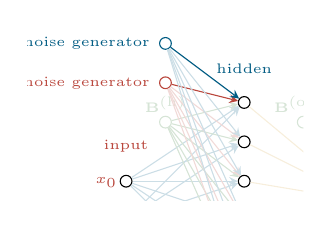
\begin{tikzpicture}
\clip (-1.25,2) rectangle + (3.5,2.2);
	\foreach \i in {0,...,1} \node[draw,circle,inner sep=1.5pt] (input\i) at (0,\the\numexpr0.5*\i+1.0+0.75) {};
	\foreach \i in {0,...,5} \node[draw,circle,inner sep=1.5pt] (hidden\i) at (1.5,\the\numexpr0.5*\i+0.75) {};
    \foreach \i in {0,...,0} \node[draw,circle,inner sep=1.5pt] (output\i) at (3.0,\the\numexpr0.5*\i+1.25+.75) {};

    % connectors input -> hidden
	\foreach \i in {0,...,1}
		\foreach \j in {0,...,5} \draw[-stealth,blue!20!white] (input\i) -- (hidden\j);

    % connectors hidden -> output
	\foreach \i in {0,...,5}
		\foreach \j in {0,...,0} \draw[-stealth,orange!20!white] (hidden\i) -- (output\j);

    % labels
	\draw (input1) ++ (0.0,0.25) node[red,above] {\tiny input};
	\draw (input0) ++ (-0.25,-0.20) node[red!100!white,above] {\tiny $x_1$};
	\draw (input1) ++ (-0.25,-0.20) node[red!100!white,above] {\tiny $x_0$};
	\draw (hidden5) ++ (0.0,0.25) node[blue,above] {\tiny hidden};
	\draw (output0) ++ (0.0,0.25) node[orange,above] {\tiny output};
	\draw (output0) ++ (0.25,-0.20) node[orange,above] {\tiny y};		
    
    % bias nodes
    \node[color=green!20!white,draw,circle,inner sep=1.5pt] (bias1) at (0.5,5*0.5+0.5) {};
	\draw (bias1) ++ (0.0,0.0) node[green!20!white,above] {\tiny $\textbf{B}^{\text{(h)}}$};
	
    \node[color=green!20!white,draw,circle,inner sep=1.5pt] (bias2) at (2.25,5*0.5+0.5) {};
	\draw (bias2) ++ (0.0,0.0) node[green!20!white,above] {\tiny $\textbf{B}^{\text{(out)}}$};

    % bias connectors
	\foreach \i in {0,...,5} \draw[-stealth,green!20!white] (bias1) -- (hidden\i);
	\draw[-stealth,green!20!white] (bias2) -- (output0);
    
	% weight labels
	\draw (input0) ++ (0.5,-1.0) node[blue!20!white,above] {\tiny $\textbf{W}^{\text{(h)}}$};
	\draw (hidden0) ++ (1.1,0) node[orange!20!white,above] {\tiny $\textbf{W}^{\text{(out)}}$};

    % noise generators
    \node[color=red!100!white,draw,circle,inner sep=1.5pt] (noise1) at (0.5,5*0.5+0.5+0.5) {};
	\draw (noise1) ++ (-1.,-0.2) node[red!100!white,above] {\tiny noise generator};
    \node[color=blue!100!white,draw,circle,inner sep=1.5pt] (noise2) at (0.5,5*0.5+0.5+1.0) {};
	\draw (noise2) ++ (-1.0,-0.2) node[blue!100!white,above] {\tiny noise generator};
    
    % noise connectors
    \draw[-stealth,red!100!white] (noise1) -- (hidden5);
    \draw[-stealth,blue!100!white] (noise2) -- (hidden5);
	\foreach \i in {0,...,4} \draw[-stealth,red!20!white] (noise1) -- (hidden\i);
	\foreach \i in {0,...,4} \draw[-stealth,blue!20!white] (noise2) -- (hidden\i);
	
	 \node[draw,color=white] (dummy) at (0,0.5) {};
\end{tikzpicture}}
                \label{neural network}
            \end{figure}
      	\endminipage\hfill
      	\minipage{0.5\textwidth}
        	\vspace{20pt}
      	    \centering
            \begin{figure}
                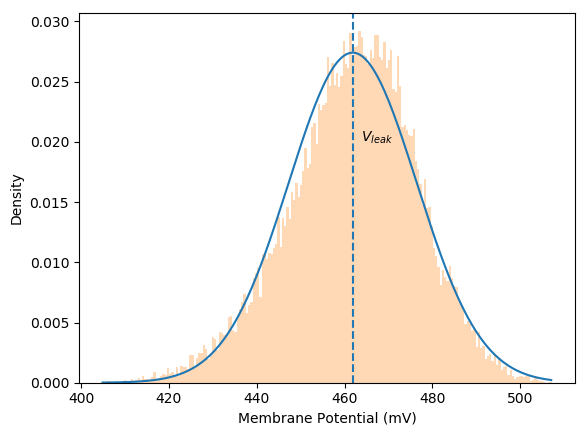
\includegraphics[scale=0.5]{mfp/activation_function_vmem_distr.png}
                \label{membrane_potential}
            \end{figure}
        \endminipage\hfill
    \end{figure}
\end{frame}

% Neuron + Threshold => spikes
\begin{frame}{Membrane Potential and Threshold}
    \begin{figure}[!htb]
    	\minipage{0.5\textwidth}
            \begin{itemize}
                \item membrane potential exceeds the threshold $\Rightarrow$ spiking
                \item fast time constants necessary
                \item $\delta V = V_{\text{leak}} - V_{\text{thres}}$
                \item transfer function $\phi$ depends on $\delta V$
            \end{itemize}
      	\endminipage\hfill
      	\minipage{0.5\textwidth}
      	    \centering
      	    \vspace{20pt}
            \begin{figure}
                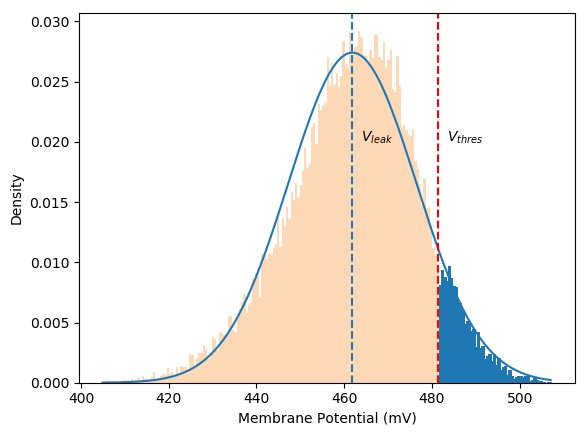
\includegraphics[scale=0.5]{mfp/activation_function_vmem_distr_with_thres.png}
                \label{membrane_potential}
            \end{figure}
        \endminipage\hfill
    \end{figure}
\end{frame}

% Neuron + input => move distr
\begin{frame}{Membrane Potential and Input}
    \begin{figure}[!htb]
    	\minipage{0.5\textwidth}
            \begin{itemize}
                \item excitatory input (Poisson spiketrain with $\sim 40 \text{kHz}$)
                \item inhibitory and excitatory noise (each $\sim 30 \text{kHz}$)
                \item weights: $w_{\text{input}} = 2 \times w_{\text{noise}}$
                \item inhibitory input for other direction
            \end{itemize}
      	\endminipage\hfill
      	\minipage{0.5\textwidth}
      	    \centering
      	    \vspace{20pt}
            \begin{figure}
            
                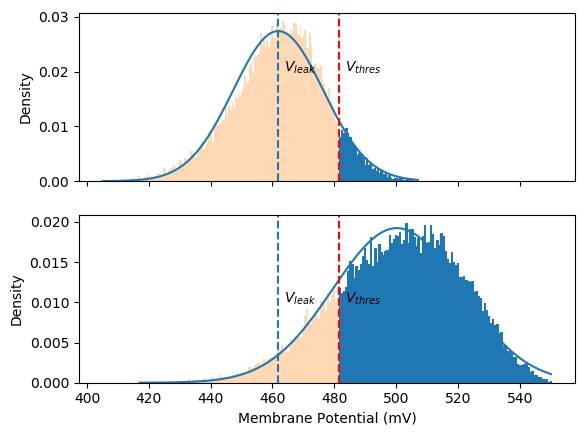
\includegraphics[scale=0.5]{mfp/activation_function_vmem_distr_with_input_with_thres.png}
                \label{membrane_potential}
            \end{figure}
        \endminipage\hfill
    \end{figure}
\end{frame}

\begin{frame}{Transfer Function on DLSv2}
    \centering
            \begin{figure}
                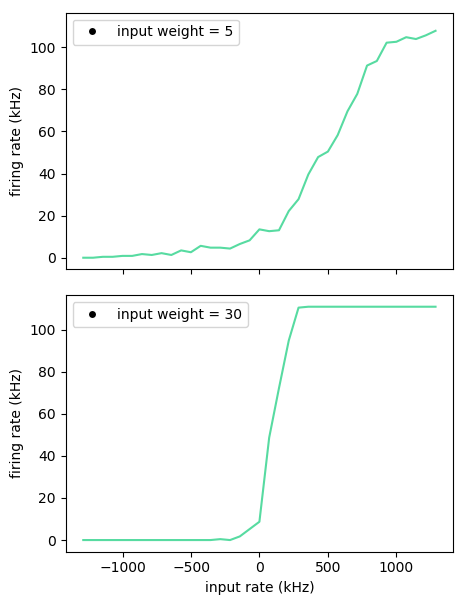
\includegraphics[scale=0.48]{mfp/uncalibrated_activation_function_input_single.png}
                \label{membrane_potential}
            \end{figure}
\end{frame}

\begin{frame}{Transfer Function on DLSv2}
    \centering
            \begin{figure}
                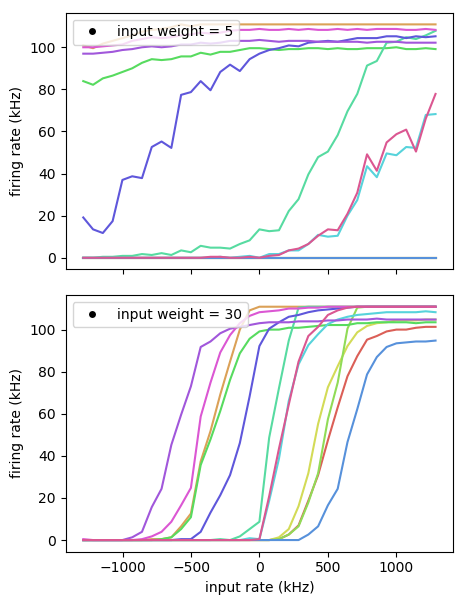
\includegraphics[scale=0.48]{mfp/uncalibrated_activation_function_input.png}
                \label{membrane_potential}
            \end{figure}
\end{frame}

\begin{frame}{Un-/Calibrated Transfer Functions}
    \begin{figure}[!htb]
    	\minipage{0.5\textwidth}
            \centering
            \textbf{uncalibrated}
            \begin{figure}
                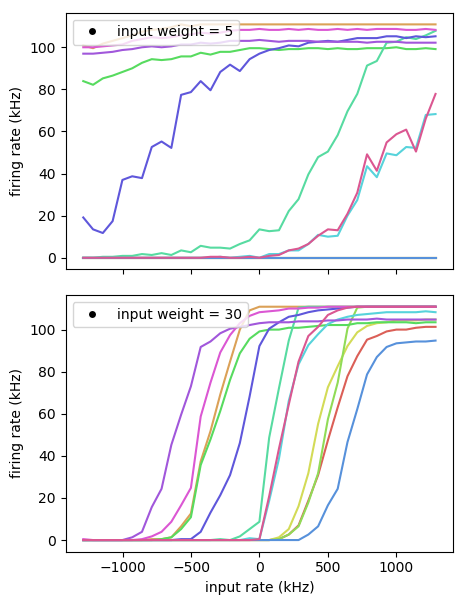
\includegraphics[scale=0.44]{mfp/uncalibrated_activation_function_input.png}
                \label{membrane_potential}
            \end{figure}
      	\endminipage\hfill
      	\minipage{0.5\textwidth}
            \centering
            \textbf{calibrated}
            \begin{figure}
                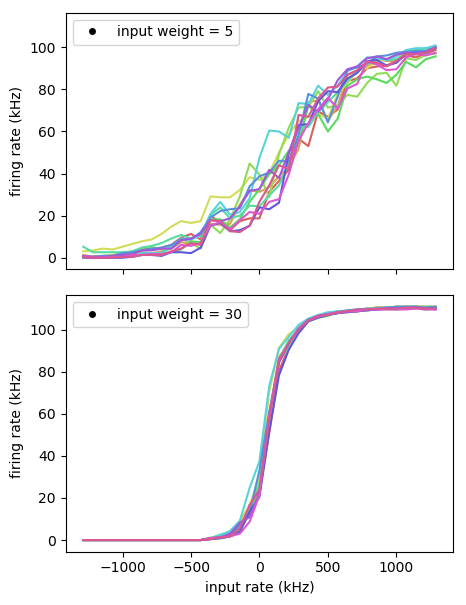
\includegraphics[scale=0.44]{mfp/calibrated_activation_function_input.png}
                \label{membrane_potential}
            \end{figure}
        \endminipage\hfill
    \end{figure}
\end{frame}

% What about Bias => move the threshold around
\begin{frame}{$V_{\text{thres}}$ as Bias}
    \begin{figure}[!htb]
    	\minipage{0.5\textwidth}
            \begin{itemize}
                \item moving $V_{\text{thres}}$ changes $\delta V$
                \item bias $b \propto \delta V $\\
                \item $b < 0 \Rightarrow $ fewer spikes $\Rightarrow$ shifted to the right
                
                \item conserves the working point of the membrane potential
            \end{itemize}
      	\endminipage\hfill
      	\minipage{0.5\textwidth}
            \centering
            \vspace{20pt}
            \begin{figure}
                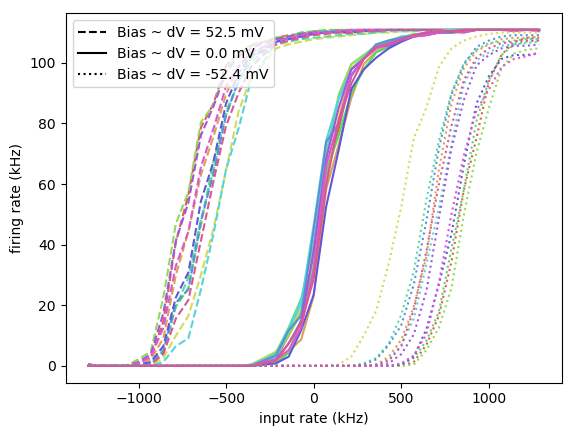
\includegraphics[scale=0.5]{mfp/bias_for_activation_function.png}
                \label{membrane_potential}
            \end{figure}
        \endminipage\hfill
    \end{figure}
\end{frame}

%%%%%%%%%%%%%%%%%%%%%%%%%%%%% LEARNING PROCESS %%%%%%%%%%%%%%%%%%%%%%%%%%%%
\section[Learning]{Deep Learning}
% What about Bias => move the threshold around
\begin{frame}{Learning Task: Circles}
    \begin{figure}[!htb]
    	\minipage{0.65\textwidth}
            \begin{itemize}
                \item feature plane: two inputs ("x" and "y")
                \item two classes:
                \begin{enumerate}
                    \item inner circle: \textbf{low} target rate $y^* = 32.6\, \text{kHz}$
                    \item outer circle: \textbf{high} target rate $y^* = 93.5\, \text{kHz}$
                \end{enumerate}
                \item find an appropriate decision-boundary
                \item on-Chip learning only
            \end{itemize}
      	\endminipage\hfill
      	\minipage{0.35\textwidth}
            \centering
            \begin{figure}
                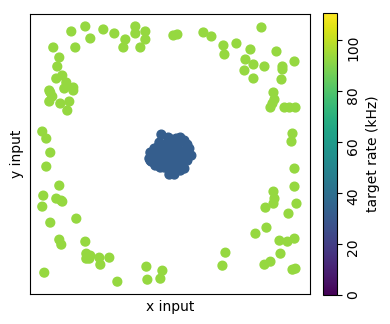
\includegraphics[scale=0.5]{mfp/targets.png}
                \label{membrane_potential}
            \end{figure}
        \endminipage\hfill
    \end{figure}
\end{frame}

\begin{frame}{On-Chip Experiment Design}
    \begin{figure}[!htb]
    	\minipage{0.6\textwidth}
    	    \textbf{Analog Core}
            \begin{itemize}
                \item $32$ LIF neurons
                \item $32 \times 32$ current based synapses
            \end{itemize}
        \textbf{PPU}
            \begin{itemize}
                \item experiment control
                \item noise and input generation
                \item update model parameters
            \end{itemize}
        
      	\endminipage\hfill
      	\minipage{0.4\textwidth}
      	\centering
      	
            \scalebox{.9}{\tikzset{block/.style={font={\sffamily\footnotesize},align=center}}%
\tikzset{box/.style={draw=black!90}}%
\tikzset{block label/.style={fill=white,font={\sffamily\footnotesize},inner sep=0.05cm}}%
\begin{tikzpicture}[
	baseline=(anc.south),
            font={\sffamily \small},
            scale=0.7,
            >=latex,
            transform shape,
	    line width=1.0\pgflinewidth,
	    anchor=center
        ]
        \pgfdeclarelayer{background layer}
        \pgfsetlayers{background layer,main}
        %\draw[use as bounding box,inner sep=0pt,draw=none] (-6.5,-3.0) rectangle ++(13,5.5);

	\node[block,box,minimum width=3.0cm,minimum height=2.0cm] (syn) at (0,0) {};
	\node[block,minimum width=3.0cm,minimum height=0.5cm,below=0.2cm of syn] (nrn) {};
	\node[block,box,minimum width=3.0cm,minimum height=0.5cm,below=0.1cm of nrn] (cm) {parameter storage};

	\node[block,minimum width=0.5cm,minimum height=2.0cm,left=0.05cm of syn] (drv) {};
	\node[block,minimum width=0.2cm,minimum height=2.0cm,left=0.05cm of drv] (padi) {};
	
	\node[block,box,minimum width=3.0cm,minimum height=0.3cm,above=0.1cm of syn] (cadc) {CADC};
	\node[block,box,minimum width=3.0cm,minimum height=0.5cm,above=0.2cm of cadc] (ppu) {PPU};

	% fitted analog core
	\node[anchor=north west,gray,rotate=90] (anc) at (cm.south east) {\scriptsize analog network core};
	\node[block,box,gray,dashed,fit={(padi) (cadc) (anc)},inner sep=0.1cm] (anc bound) {};

	% digital control and events
	\node[block,box,anchor=south east,minimum width=1.7cm,minimum height=0.8cm] (event)
		at ($(nrn.south west -| anc bound.west) + (-0.2,0.2)$) {Event \\ Handling};
	\node[block,box,anchor=south east,minimum width=2.2cm,minimum height=0.4cm] (link)
		at ($(anc bound.south west) - (0.2,0.0)$) {I/O};
	\node[block,box,anchor=north east,minimum width=1.7cm,minimum height=1.2cm] (mem)
		at ($(anc bound.north west) - (0.2,0.0)$) {Config.\\Memory\\Controllers};

	\foreach \x in {0,1,...,5} {
		\draw[] (nrn.south west) ++ (\x*0.5,0.0) ++ (0.25,0.25) circle (0.2cm);
		\draw[gray,latex-] (syn.south west) ++ (\x*0.5+0.25,-0.22) -- ++(0.0,2.22);
		
		\foreach \y in {0,1,...,3}
			\draw[gray] (syn.south west) ++ (\x*0.5+0.25,0.25+\y*0.5) circle (0.02cm);
	}

	\foreach \y in {0,1,...,3} {
		\draw[] (drv.south west) ++ (0.0,\y*0.5) ++ (0.1,0.05) -- ++(0.0,0.4) -- ++(0.3,-0.2) -- cycle;
		\draw[gray] (syn.south west) ++ (-0.1,\y*0.5+0.25) -- ++(3.0,0.0) -- ++(0.1,0.0);
	}

	% arrows
	\draw ($(event.east |- drv.south west) + (0.0,0.25)$) -- ($(drv.south west) + (-0.2,0.25)$) -- ++(0.0,1.5);
	\draw[,latex-] (event.east |- nrn.west) -- (nrn.west);
	\draw[,latex-latex] (link.north -| event) -- (event);
	\foreach \y in {0,1,...,3}
		\draw[latex-,line cap=rect] (drv.south west) ++ (0.1,\y*0.5+0.25) -- ++(-0.3,0.0);

	\draw[latex-latex] (event.west) -- ++(-0.25,0.0) coordinate (x) -- (link.north -| x);
	\draw[-latex] (x) -- (x |- ppu) -- (ppu);
	\draw[-latex] (x) -- (x |- mem) -- (mem);
	\draw[-latex] (mem.east) ++ (0.0, 0.1) -- ++(0.2,0.0);
	\draw[latex-] (mem.east) ++ (0.0,-0.1) -- ++(0.2,0.0);
	
	% labels
	\node[block label] at (syn) {synapse array};
	\node[block label] at (nrn) {neurons};
  \end{tikzpicture}
}
        
            \begin{figure}
                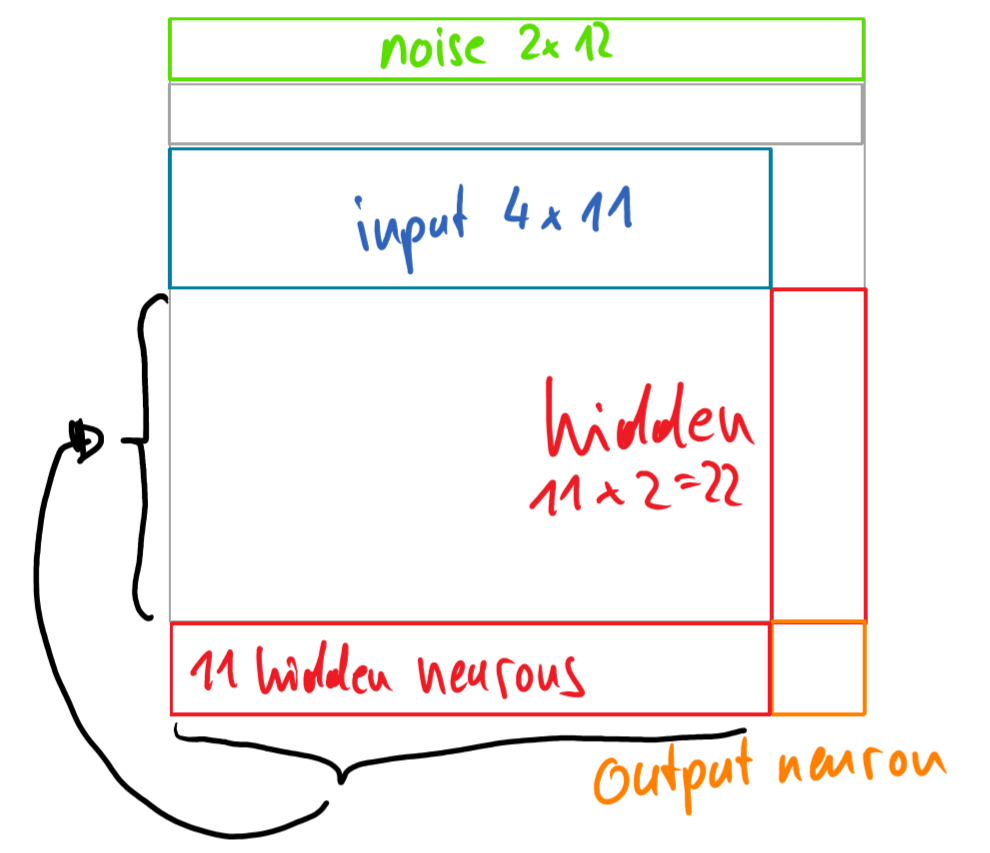
\includegraphics[scale=0.22]{mfp/synapse_array_transparent.png}
                \label{membrane_potential}
            \end{figure}
        \endminipage\hfill
    \end{figure}
\end{frame}

% Performance
\begin{frame}{Learning Performance}
\begin{figure}[!htb]
	\minipage{0.65\textwidth}
        \begin{figure}
            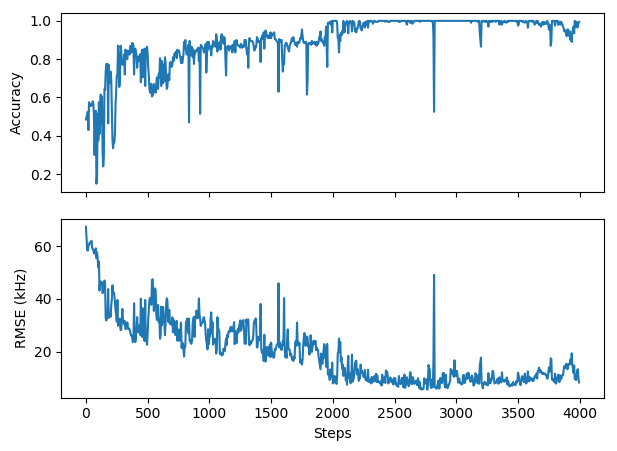
\includegraphics[scale=0.6]{mfp/learning_process/learning_performance.png}
        \end{figure}
  	\endminipage\hfill
  	\minipage{0.35\textwidth}
  	\centering
        target
        \begin{figure}
            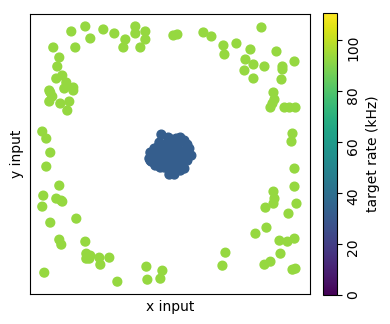
\includegraphics[scale=0.25]{mfp/targets.png}
            \label{fig:my_label}
        \end{figure}
        output
        \begin{figure}
            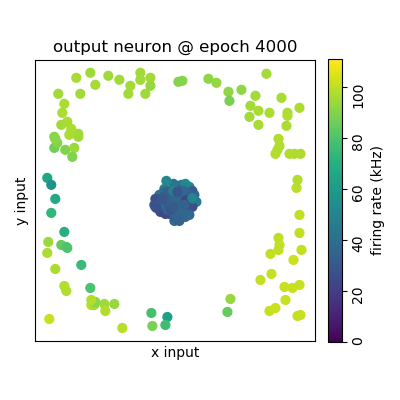
\includegraphics[scale=0.25]{mfp/output_neuron_4000.png}
            \label{fig:my_label}
        \end{figure}
    \endminipage\hfill
\end{figure}
\end{frame}

\section[Summary]{Summary}

\begin{frame}{Conclusion and Outlook}
\begin{figure}[!htb]
	\minipage{0.7\textwidth}
        \textbf{Circles}
            \begin{itemize}
                \item performance with shorter measurement period
                \item controlled decalibration
                \item stability: better choice of system parameters
                \item implementation on HICANN-X
            \end{itemize}
        \textbf{SuperSpike}
        \begin{itemize}
            \item prototype implementation on HICANN-X (computation via host)
            \item implement host computation on-chip
            \item on-chip only possible with next tape-out (Spring 2020)
        \end{itemize}
  	\endminipage\hfill
  	\minipage{0.3\textwidth}
  	\centering
        \begin{figure}
            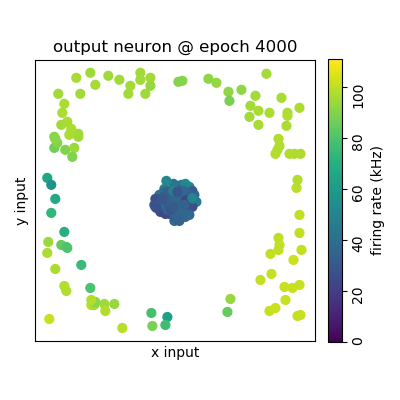
\includegraphics[scale=0.3]{mfp/output_neuron_4000.png}
            \label{fig:my_label}
        \end{figure}
    \endminipage\hfill
\end{figure}
\end{frame}

\appendix

\begin{frame}[fragile]{Backup slides}
\centering
        \begin{figure}
            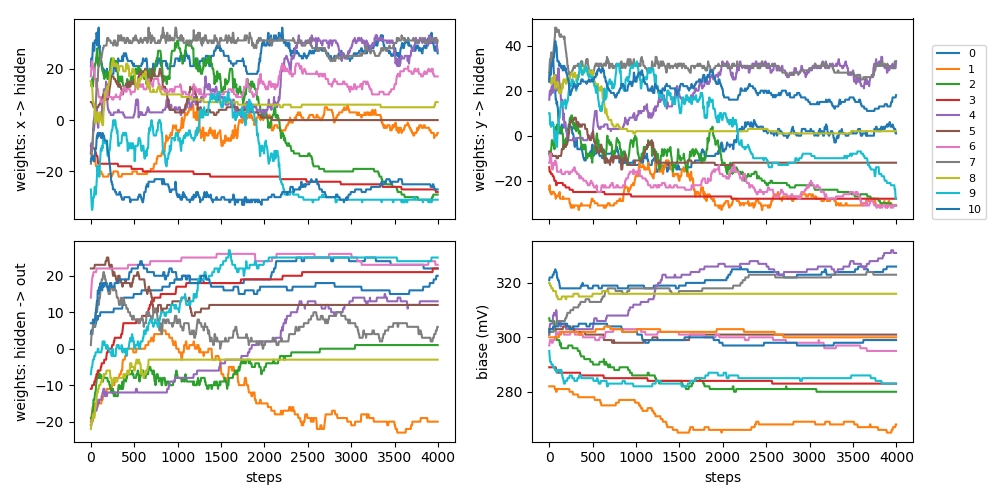
\includegraphics[scale=0.5]{mfp/model_parameters.png}
            \label{fig:my_label}
        \end{figure}
\end{frame}

\begin{frame}[fragile]{Backup slides}
\centering
        \begin{figure}
            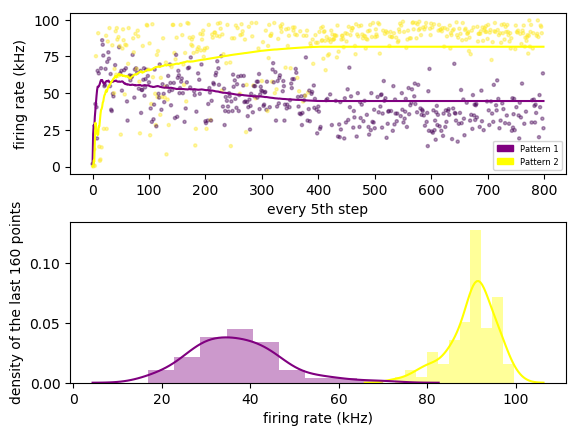
\includegraphics[scale=0.65]{mfp/rates_dist.png}
            \label{fig:my_label}
        \end{figure}
\end{frame}

\begin{frame}[fragile]{Backup slides}
\textbf{Hardware Parameters}
\begin{itemize}
    \item $\tau_{\text{syn\_exc}}$ = 1e-5 s
    \item $\tau_{\text{mem}}$ = 5e-7 s
    \item $\tau_{\text{refrac}}$ = 9e-6 s
    \item PulseLength = 1
    \item Mmnt periode = 2.3 ms
\end{itemize}
\end{frame}
  	
\end{document}